  \documentclass[11pt]{article}
\usepackage{debulletin}
%\usepackage{deauthor}
\usepackage{times}
\usepackage{epsfig}
%\usepackage{subfigure}
\usepackage{wrapfig}
\usepackage{color}
\usepackage{boxedminipage}
\usepackage{graphicx}
\usepackage{url}
\usepackage{tabu}
\usepackage{multirow}
\usepackage{ulem}
\usepackage{layouts}
\usepackage[utf8]{inputenc}
\usepackage{paralist}
%\usepackage{thmtools} 
\usepackage{thm-restate}
\usepackage{dsfont}
%\usepackage{amsthm}
\usepackage{amsmath}
\usepackage{amssymb}
\usepackage{amsfonts}
\usepackage{hyperref}
\usepackage{enumitem}
\usepackage{xspace}
\usepackage{tikz}
\usepackage[T1]{fontenc}
\usepackage{beramono}
\usepackage{listings}
\usepackage{xcolor}
\usepackage{graphics}
\usepackage{pifont}
\usepackage{algorithmic}
\usepackage[sort&compress,numbers]{natbib}
\usepackage{microtype}
\usepackage{booktabs}
\usepackage{pgfplotstable}
\usepgfplotslibrary{groupplots}
\usepackage{bbm}
\usepackage{verbatim}
\usepackage{caption}
\usepackage{subcaption}
\usepackage{siunitx}
\usepackage[autostyle, english=american]{csquotes}
\usepackage{breakurl}
\usepackage{makecell}
\usepackage{changepage}
\usepackage{diagbox}
\usepackage{etoolbox}
\usepackage{float}
\usepackage{array}
\usepackage{tabularx}
\usepackage{colortbl}
\usepackage[english]{babel}
\usepackage[edges]{forest}
\usepackage{xfrac}
\usepackage{mdwlist}
\usepackage{arydshln}
\usepackage{adjustbox}
\usepackage{longtable}
\usepackage{comment}
\usepackage{svg}
\usepackage[vlined,ruled,linesnumbered]{algorithm2e}
\usepackage{bm}
\usepackage[noend]{algpseudocode}
\usepackage{soul}
\usepackage{makecell}
\usepackage{cleveref}
\usepackage{grffile}
\usepackage{tablefootnote}
\usepackage{threeparttable}
\usepackage{bibentry}
\usepackage{cancel}
\usepackage[sectionbib]{chapterbib}

\DeclareMathOperator*{\argmin}{argmin} 
\DeclareMathOperator*{\argmax}{argmax} 
% \newcommand{\xhdr}[1]{{\vspace{1pt}\noindent\bfseries #1}.}
% \newcommand{\ie}{\textit{i.e., }}
% \newcommand{\eg}{\textit{e.g., }}
% \newcommand{\etal}{\textit{et al.}}
% \newcommand{\etc}{\textit{etc.}}
% \newcommand{\wrt}{\textit{w.r.t. }}
% \newcommand{\cf}{\textit{cf. }}
% \newcommand{\aka}{\textit{aka. }}
% \newcommand{\CITE}{\textcolor{blue}{(CITE)}}
% \newcommand{\rex}[1]{\textcolor{magenta}{(Rex: #1)}}
% \newcommand{\jialin}[1]{\textcolor{olive}{(Jialin: #1)}}

\definecolor{citecol}{HTML}{2DDC0E}
\definecolor{tableofcontent}{HTML}{E63E15}
\definecolor{urlcol}{HTML}{2470D8}
\usepackage{hyperref}
\hypersetup{
    colorlinks=true,       % false: boxed links; true: colored links
    linkcolor=tableofcontent, 
    citecolor=citecol,        % color of links to bibliography
    %filecolor=blue,      % color of file links
    urlcolor=black,           % color of external links
}


\newcolumntype{L}[1]{>{\raggedright\let\newline\\\arraybackslash\hspace{0pt}}m{#1}}
\newcolumntype{C}[1]{>{\centering\let\newline\\\arraybackslash\hspace{0pt}}m{#1}}
\newcolumntype{R}[1]{>{\raggedleft\let\newline\\\arraybackslash\hspace{0pt}}m{#1}}

\newenvironment{CompactEnumerate}{
\begin{list}{\arabic{enumi}.}{%
\usecounter{enumi}
\setlength{\leftmargin}{14pt}
\setlength{\itemindent}{1pt}
%\setlength{\topsep}{-1pt}
\setlength{\itemsep}{1pt}
}}
{\end{list}}

\newenvironment{CompactItemize}{
\begin{list}{$\bullet$}{%
\setlength{\leftmargin}{14pt}
\setlength{\itemindent}{0pt}
%\setlength{\topsep}{-1pt}
\setlength{\itemsep}{0pt}
}}
{\end{list}}

\begin{document}


% please enter real date, vol no, issue no
\bulletindate{December 2023}
\bulletinvolume{47}
\bulletinnumber{4}
\bulletinyear{2023}

% these are files that I have- but your part of the issue can be done without
% them
\IEEElogo{cs.pdf}
\insidefrontcover{incvA19.pdf}
%\insidebackcover[ICDE Conference]{./calls/icde-new-a.ps}

\begin{bulletin}

% the above samples assume the issue is generated from a directory structure of the following sort
% major directory name is month and year of issue
% there are sub-directorys for
% letters: directory name is "letters"
% technical articles: a directory per paper, named for an "author"
% news articles: directory name is "news"
% calls: directory name is "calls

%
%  Editor letters section.  Use the lettersection environment.
%  Each letter is contained in a letter environment, where the two required
%  options to \begin{letter} are the author and the address of the author.
%

\begin{lettersection}

% there will be other letters- and a blank page will appear in your document
% but the special issue part will be fine

\begin{letter}{Letter from the Editor-in-Chief}
 {Haixun Wang}{Instacart}
 \documentclass[11pt]{article} 

\usepackage{deauthor,times,graphicx}
%\usepackage{url}
\usepackage{hyperref}

\begin{document}

This special issue of the IEEE Data Engineering Bulletin is dedicated to a timely subject: high-dimensional similarity searches. 

High-dimensional similarity searches are indispensable in a variety of fields. For instance, they are employed for time series analysis and forecasting, which have numerous applications in science, medicine, and business. Recently, the subject of vector databases has garnered significant attention, primarily driven by the emergence of Large Language Models (LLMs) and Retrieval Augmented Generation (RAG), where  vector databases have assumed a crucial role in facilitating various applications in the domain of generative AI ranging from  chatbots to AI agents. On the other hand, the continuous progress and widespread adoption of vector databases have been occurring over the past few decades. Specifically, it brought about a revolution in the domain of information retrieval by enhancing the traditional approach of term-based retrieval with embedding-based retrieval. This novel technique, which involves utilizing vector-based semantic search, significantly enhances the ability to retrieve relevant information. 

This special issue, curated by Associate Editor Themis Palpanas,  gathers insights from various branches of this field. The articles contained within this special issue provide an array of theoretical and practical solutions for similarity searches in high-dimensional spaces. Our authors investigate algorithms to improve similarity searches, explore the evolution of graph-and tree-based indexes, and chart the course for improving data management systems. The articles delve into aspects of optimal design strategies to enhance computational efficiency in the era of AI, examine the deployment of techniques like locality-sensitive hashing and product quantization, and delve into the improvements dynamic space partitions can offer for faster and more accurate searches.

We believe the topic of vector databases is significant for the database community, for its role as a bridge connecting data management and artificial intelligence.  While considerable progress has been made in the field of vector-based similarity search, it is crucial to recognize the existence of ongoing obstacles that require attention and resolution. For example, there exist numerous relationships among the vast amount of data represented by the vector database. Given a question, how do we ensure all pertinent information is retrieved through vector search?  Additionally, what strategies can be employed to narrow the disparity between pre-training an LLM on the vast amount of data and in-context learning via RAG, which disregards the majority of the data that could potentially have relevance to the given question? Thus, our shared objective is to enhance the advancement of this discipline, and our overarching aspiration encompasses two expansive domains: database and artificial intelligence. 

We would like to express our profound gratitude to all the authors who contributed to this issue, to Themis Palpanas for bringing these insightful articles to the forefront, and to Nurendra Choudhary for his assistance in the publication process.


\end{document}


\end{letter}

\newpage


\newpage

%
%% your introductory letter goes here
%
%\begin{letter}{Letter from the Special Issue Editor}
\begin{letter}{Letter from the Special Issue Editors} %JF: made it editors, plural
%\setcounter{section}{0}
{Xin Luna Dong$^*$, Alon Halevy$^\dagger$, Shane Moon$^*$}{$^*$Meta (Facebook),$^\dagger$Amazon}
\documentclass[11pt]{article}

\usepackage{deauthor,times,graphicx}
%\usepackage{url}

\begin{document}
How convenient would it be to have an AI assistant to share the latest updates for your favorite sports team, or to present you the recent sales trend for your business with a single natural language query. Retrieval Augmented Generation (RAG), bringing latest and targeted information into Large Language Models (LLMs), makes this desire come true. 

How to build a RAG system for trustworthy Question Answering (QA)? Some of the challenges that we need to solve are the following. First, we shall evaluate and debug RAG systems to draw insights and iterate quickly. How to measure the quality of RAG systems? How to conduct evaluation with minimum manual efforts and affordable costs? How to do error attribution easily so that we can understand the system and iterate development quickly? Second, we need to conduct retrieval effectively and efficiently. For a given query, shall we trigger retrieval or leave it to the LLM to answer? How do we retrieve information effectively from different sources: unstructured text, structured text, multi-modal data? How to handle ambiguity and context understanding? And how to achieve all the above within a given latency and computation budget? Last but not the least, we need to be able to use the retrieved information effectively to power answer generation. An ideal RAG system should be able to provide correct answers when useful information is retrieved without adding any hallucination. Practically, this requires selecting and/or ranking relevant information from large volumes of data, oftentimes with the presence of irrelevant, noisy, or even conflicting information, to fit in the context window. 

This issue collects a set of papers around RAG shedding lights on how to address the aforementioned challenges. We start with two papers for addressing the first challenge – evaluation: {\bf Yang et al.} provided an overview and reflection for the {\it KDD Cup 2024 CRAG Challenge}. It discussed the rationale behind the benchmark and challenge design, highlighted the winning solutions, and shared learnings from hosting a large-scale challenge for RAG. {\bf Liu et al.} introduced {\it GraphEval} for large-scale factuality evaluation. It attempted to address the scalability and domain-agnostic challenges in existing evaluation methods, by integrating KGs for question generation and a lightweight judge model for evaluation. We then present 2 papers focusing on the second challenge – retrieval: {\bf Reddy et al.} introducing {\it ReFit}, a method to leverage re-ranker to improve retriever’s recall in a Retrieval - Reranking pipeline. {\bf Christmann et al.} presents the {\it Quasar} system for QA over unstructured text, structured tables, and knowledge graphs, with unified treatment of all sources and innovative design for question understanding and evidence re-ranking. Finally, we offer 4 papers for building RAG systems from different angles and also discussing the third challenge. {\bf Tang et al.} introduced {\it Symphony}, a system designed for trustworthy QA over multimodal data lakes, aiming to use RAG to improve QA system’s accuracy via reasoning and verification. The next two papers focused on understanding Knowledge Graphs (KGs) with RAG: {\bf Sequeda et al.} tried to understand to what extent KGs can increase the accuracy of LLM-powered QA systems, on SQL databases in particular. {\bf Yang et al.} discuss the {\it co-learning} of KGs and LLMs, through LLM-aided KG construction, KG-guided LLM enhancement, and knowledge-aware multi-agent federation, emphasizing the RAG paradigm, towards fully utilizing the value of complex data. The last paper is by {\bf Rahman et al.}, which proposed to shift from a “fast, intuitive thinking” system to a “slow, deliberate, analytical thinking” to improve RAG in complex enterprise applications. 

Overall, the above papers represent an interesting sample of the ongoing work on the recent research on RAG. We hope that this special issue will further help and inspire the research community in its quest to solve this challenging problem. We would like to thank all the authors for their valuable contributions, as well as Haixun Wang for giving us the opportunity to put together this special issue, and Nurendra Choudhary for his help in its publication.

\end{document}

\end{letter}

\end{lettersection}
\begin{opinionsection}
    \setcounter{section}{0}
    \begin{opinion}{A Summary of ICDE 2022 Research Session Panels}{Zhifeng Bao, Panagiotis Bouros, Reynold Cheng, Byron Choi, Anton Dign\"{o}s, Wei Ding,Yixiang Fang, Boyang Han, Jilin Hu, Arijit Khan, Wenqing Lin, Xuemin Lin, Cheng Long, Nikos Mamoulis, Jian Pei, Matthias Renz, Shashi Shekhar, Jieming Shi, Eleni Tzirita Zacharatou, Sibo Wang, Xiao Wang, Xue Wang, Raymond Chi-Wing Wong, Da Yan, Xifeng Yan, Bin Yang, Dezhong Yao,Ce Zhang, Peilin Zhao, Rong Zhu}{}
    \documentclass{article}

\usepackage{deauthor}

\usepackage{latexsym}
\usepackage{graphicx}
\graphicspath{{./images/}}
\usepackage{booktabs} % for formal tables
\usepackage{color}  % for coloring text
\usepackage{amsmath}  % for aligning equations
\usepackage{subcaption}
\usepackage{caption}
\usepackage{tikz}
\usepackage{colortbl} % for color in tables
\usepackage{framed}
\usepackage{multirow}
\usepackage{multicol}
\usepackage{hyperref}
\usepackage{url}
\usepackage{balance}
\usepackage{verbatim}
\usepackage{cancel}
\usepackage{xspace} % for correcting space after macro commands
\usepackage{algorithm2e}
\usepackage{bbold} % for writing mathbb{1}
\usepackage{balance}
\usepackage{stmaryrd}
\usepackage{enumitem}
\usepackage{array} % package for hiding a column
\usepackage{bold-extra} % to enable textbf with textsc

% used for making text readable in document and .tex
% \setlength{\parindent}{0pt}

\newcommand{\struct}[1]{\texttt{\small #1}}
\newcommand{\utterance}[1]{\textit{#1}}
\newcommand{\phrase}[1]{\textit{``#1''}}

% \newcommand {\g}[1]{\textcolor[gray]{0.6}{#1}}

\newcommand{\drop}{\dag\xspace}

\newenvironment{Snugshade}[1][236,236,236]{
    \setlength{\itemsep}{0pt}
     \setlength{\parsep}{0pt}
     \setlength{\topsep}{0pt}
     \setlength{\partopsep}{0pt}
     \setlength{\leftmargin}{1.5em}
     \setlength{\labelwidth}{0em}
     \setlength{\labelsep}{0em} 
    \setlength{\parskip}{0pt}
    \definecolor{shadecolor}{RGB}{#1}
    \begin{snugshade}
}{
    \end{snugshade}
}


\newcommand{\method}{\textsc{Quasar}\xspace}
\newcommand{\benchmark}{\textsc{PerQA}\xspace}
\newcommand{\itemslist}[1]{$\langle$\struct{#1}$\rangle$}


\newcommand{\convinse}{\textsc{Convinse}\xspace}
\newcommand{\explaignn}{\textsc{Explaignn}\xspace}
\newcommand{\clocq}{\textsc{Clocq}\xspace}
\newcommand{\unikqa}{\textsc{UniK-Qa}\xspace}
\newcommand{\gptthree}{\textsc{Gpt-3}\xspace}
\newcommand{\gptfour}{\textsc{Gpt-4}\xspace}
\newcommand{\llama}{\textsc{Llama3}\xspace}
\newcommand{\spaghetti}{\textsc{Spaghetti}\xspace}


\newcommand{\compmix}{\textsc{CompMix}\xspace}
\newcommand{\timequestions}{\textsc{TimeQuestions}\xspace}
\newcommand{\crag}{\textsc{Crag}\xspace}


\newcommand{\squishlist}{
    \begin{list}{$\bullet$}{
        \setlength{\itemsep}{0pt}
	\setlength{\parsep}{3pt}
	\setlength{\topsep}{3pt}
	\setlength{\partopsep}{0pt}
	\setlength{\leftmargin}{1.5em}
	\setlength{\labelwidth}{1em}
	\setlength{\labelsep}{0.5em}
    }
}

\newcommand{\squishend}{
    \end{list}
}

\newcommand{\myparagraph}[1]{\vspace*{0.2cm}\noindent \textbf{#1}.}
\newcommand{\myparagraphnospace}[1]{\noindent \textbf{#1}.}

% \newcommand{\GW}[1]{\emph{{\color{blue} GW:#1}}}
% \newcommand{\PC}[1]{\emph{{\color{orange} PC: #1}}}
% \newcommand{\tocite}{{{\color{red} [CITE]}}}


\begin{document}

\title{RAG-based Question Answering \\ over Heterogeneous Data and Text}

\author{
Philipp Christmann,
Gerhard Weikum\\\\
Max Planck Institute for Informatics\\
Saarland Informatics Campus, Germany\\
\texttt{\{pchristm, weikum\}@mpi-inf.mpg.de}}

\maketitle

\section*{Abstract}
This article presents the \method system for question answering over unstructured text, structured tables, and knowledge graphs, with unified treatment of all sources.
The system adopts a RAG-based architecture, with a pipeline of evidence retrieval followed by answer generation, with the latter powered by a 
moderate-sized
language model.
Additionally and uniquely, \method
has components for question understanding, to derive crisper input for evidence retrieval, and for re-ranking and filtering the retrieved evidence before feeding the most informative pieces into the answer generation.
Experiments with three different benchmarks demonstrate the high answering quality of our approach, being on par with or better than large GPT models, while keeping the computational cost and energy consumption orders of magnitude lower.

\label{sec:intro}
\section{Introduction}

\noindent\textbf{Motivation and Problem.} The task of question answering, QA for short, arises in many flavors: factual vs. opinions, simple lookups vs. multi-hop inference, single answer vs. list of entities, 
direct answers vs. long-form, one-shot questions vs. conversations, and other varieties 
(see, e.g., surveys~\cite{RogersGA:CS2023,RoyAnand:MC2021}).
The state-of-the-art for this entire spectrum has been greatly advanced in the past decade. Most notably, incorporating deep learning into retriever-reader architectures (e.g.,~\cite{DBLP:conf/acl/ChenFWB17,DBLP:conf/eacl/IzacardG21,DBLP:conf/emnlp/KarpukhinOMLWEC20}) has boosted answering quality, and most recently, large language models (LLM)~\cite{Minaee-LLM-survey,Zhao-LLMsurvey} have pushed the envelope even further (e.g.,~\cite{DBLP:journals/arXiv/abs-2305-06984}).

% strengths and limitations of LLM for QA
Today’s LLMs alone are capable of accurately answering many \textit{factoid} questions, simply from their pre-trained parametric memory which latently encodes huge text corpora and other online contents.
However, this critically depends on the frequency of evidence in the underlying contents and the complexity of the information need. 
For example, 
asking for the {\em MVP of the 2024 NBA season} would easily return the correct answer Nikola Jokic, 
but asking for the {\em highest-scoring German NBA player} or the {\em MVP of the 2024 German basketball league} pose a big challenge.
The reason is that LLMs alone do not easily recall information about not so popular or even long-tail entities~\cite{Kandpal:ICML2023,Sun:NAACL2024},
and that they are mainly geared for direct look-ups as opposed to connecting multiple pieces of evidence~\cite{Mavi:FnT2024,Zhang:NAACL2024}.

% introduce RAG and discuss need for heterogeneous sources
\cite{DBLP:journals/arXiv/abs-2312-10997,Guu-REALM:ICML2020,DBLP:conf/nips/LewisPPPKGKLYR020,Zhao:arxiv2024}
known as RAG, address these bottlenecks. In addition to cleverly crafted prompts and few-shot examples, the LLM is provided with the top-ranked results of an explicit retrieval step, like web search or knowledge graph (KG) lookups. The former is often necessary for freshness of answers, and the latter may help with long-tail entities and also mitigate the notorious risk of hallucinations. Still, this generation’s RAG architectures are limited in how broad and how deep they tap into external sources. Popular AI assistants like Gemini or ChatGPT seem to primarily retrieve from the text of web pages (incl. Wikipedia articles), and academic research has additionally pursued knowledge augmentation by enhancing prompts with facts from large KGs (e.g., Wikidata).

An additional content modality that is still underexplored are {\em online tables}: a wide range of tabular data including HTML tables in web pages, spreadsheets and statistics, all the way to CSV and JSON datasets that are abundant on the Internet. There is prior work on joint support for text and KGs and for text and tables, but very little on all of these together -- some notable exceptions being~\cite{Christmann-CONVINSE:SIGIR2022,Christmann-Explaignn:SIGIR2023,Oguz-UniK-QA:NAACL2022,Zhang-Spaghetti:ACL2024}.


\noindent\textbf{Examples.} All three heterogeneous types of sources are crucial not only for answering different questions from different kinds of evidence, but also for combining multiple pieces of evidence of different modalities to infer correct and complete answers.
To 
illustrate
the need for tapping all sources, consider the following questions:

% \vspace*{0.2cm}
\begin{quote}
$Q1$: \utterance{Which Chinese basketballers have played in the NBA?}\\
 \indent $Q2$: \utterance{Who was the first Chinese NBA player?}\\
  \indent $Q3$: \utterance{Which Chinese NBA player has the most matches?}
\end{quote}
% \vspace*{0.2cm}

Q1 can be cast into querying a KG, but the list there is not necessarily complete and up-to-date, so additional evidence from text or tables would be desired. 
Q2 needs information about who played in which seasons, found only in web pages or sports-statistics tables. 
Finally, Q3 may be lucky in finding prominent textual evidence (e.g., in biographies, Wikipedia etc.), but this often faces divergent statements, and resolving contradictions needs to dive into more evidence. Besides, when textual evidence is rare and hard to find or not trustworthy enough, then information from multiple tables and text snippets may have to be aggregated (e.g., totals of per-season counts).
Some of this may perhaps become feasible for an industrial LLM’s RAG capabilities in the near future, but there are always harder scenarios by moving from Chinese NBA players deeper into the long tail, such as asking for {\em Lithuanian players in the German handball league}.

\vspace*{0.2cm}
\noindent\textbf{Approach and Contribution.} This paper presents a simple but powerful and versatile RAG system with unified access to text, KG and tables. We call our method {\em \method} 
(for Question Answering over Heterogeneous Sources with Augmented Retrieval).
Its architecture is relatively straightforward: all heterogeneous content is verbalized and indexed for retrieval; a retriever finds top-ranked results for the given question (from different source types), and these are fed into the LLM for answer generation. This is the unsurprising bird-eye’s view. Specific details that are key factors for the strong performance of \method are: 

\squishlist
\item[i)] automatically casting user questions into a structured representation of the information need, which is then used to guide 
\item[ii)] judicious ranking of search results, with multiple rounds of re-ranking and pruning, followed by
\item[iii)]	extracting faithful answers from an LLM in RAG mode, with answers grounded in tangible evidence.
\squishend


\vspace{0.2cm}
\noindent The paper presents experiments with three different benchmarks, covering various flavors of questions.
We focus on one-shot questions; conversational QA is out of scope here, but \method itself is well applicable to this case, too.
Our experiments demonstrate that our methods are competitive, on par with big GPT models and often better,
while being several orders of magnitude lower in computational and energy cost.
The experimental findings also highlight that question understanding, with structured representation of user intents, and iterative re-ranking of evidence are crucial for good performance.

Overall, our contribution lies in proposing a unified system architecture for RAG-based question answering over a suite of different data sources, with strong points regarding both effectiveness (i.e., answer quality)
and efficiency (i.e., computational cost).


\label{sec:background}
\section{Related Work}

The RAG paradigm came up as a principled way of enhancing LLM factuality incl. provenance and mitigating the risk of hallucination~\cite{Guu-REALM:ICML2020, DBLP:conf/nips/LewisPPPKGKLYR020}.
It is highly related to the earlier
retriever-reader architectures for QA~\cite{DBLP:conf/acl/ChenFWB17,DBLP:conf/emnlp/KarpukhinOMLWEC20}, especially when the reader uses the fusion-in-decoder method~\cite{DBLP:conf/eacl/IzacardG21,Oguz-UniK-QA:NAACL2022}.
Since its invention, RAG methodology has been greatly advanced, introducing a wide suite of extensions, such as batched inputs, interleaving retrieval and generation steps, and more (see the recent surveys~\cite{DBLP:journals/arXiv/abs-2312-10997,Zhao:arxiv2024}).

On question answering (QA), there is a vast amount of literature including a wealth of differently flavored benchmarks (see, e.g.,~\cite{RogersGA:CS2023}).
The case of interest here is QA over heterogeneous sources, tapping into both unstructured content and structured data. 
A variety of works has pursued this theme by combining knowledge graphs with text sources, using graph-based methods, neural learning and  language models (e.g.,~\cite{Pramanik-Uniqorn:JWS2024,Sun-PullNet:EMNLP2019,Yasunaga:NAACL2021}).

Most relevant for this article is the research on jointly leveraging all different sources: text, KGs, and tables (incl. CSV and JSON files). This includes  
the \unikqa system~\cite{Oguz-UniK-QA:NAACL2022},
the \spaghetti/SUQL project~\cite{Liu-SUQL:NAACL2024,Zhang-Spaghetti:ACL2024},
the \textsc{Matter} method~\cite{Lee-MATTER:ACL2024},
the STaRK benchmarking~\cite{Wu-STARK:arxiv2024},
and our own prior work
~\cite{Christmann-CONVINSE:SIGIR2022,Christmann-Explaignn:SIGIR2023} (without claiming exhaustiveness).
Out of these, we include \unikqa, \spaghetti and our own systems \convinse and \explaignn as baselines in the experimental evaluation.
Their architectures are similar to ours, but \unikqa and \spaghetti do not have our distinctive elements of
question understanding and iterative re-ranking (originally introduced in \explaignn~\cite{Christmann-Explaignn:SIGIR2023}).

\label{sec:method}
\section{Methodology}

\begin{figure}[tb]
  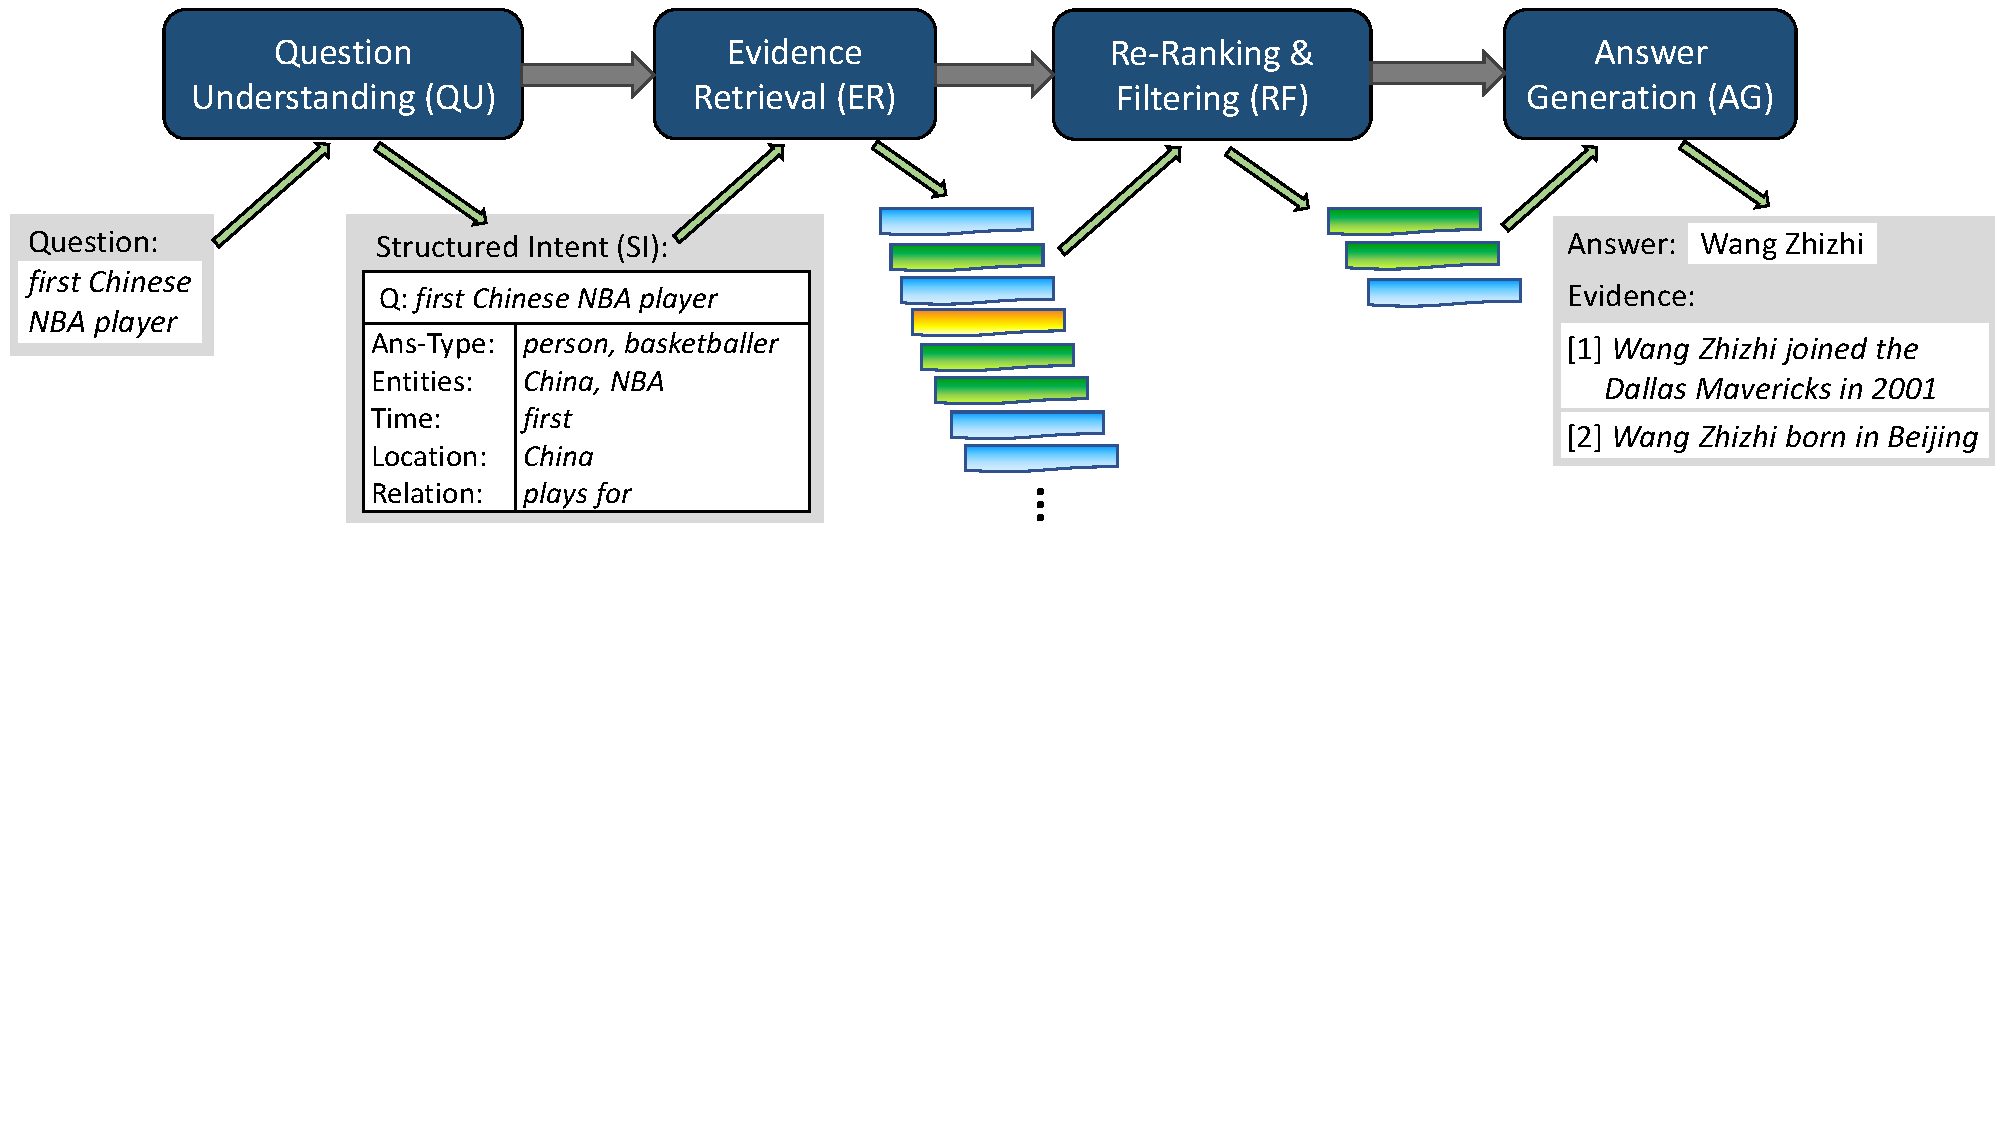
\includegraphics[width=\textwidth]{submissions/Gerhard2024/figures/compass-overview.pdf}
  \caption{Overview of the \method system.}
  \label{fig:compass-overview}
\end{figure}

% start with system overview
The \method system is a pipeline of four major stages, as illustrated in Figure \ref{fig:compass-overview}.
First, the input question is analyzed and decomposed, in order to compute a {\em structured intent (SI)} representation that will pass on to the subsequent steps, along with the original question. Second, the SI is utilized to retrieve pieces of evidence from different sources: text, KG and tables. 
Third, this pool of potentially useful evidence is filtered down, with iterative re-ranking, to arrive at a tractably small set of most promising evidence.
The final stage generates the answer from this evidence,
passing back the answer as well as evidence snippets for user-comprehensible explanation.

The second and fourth stage, Evidence Retrieval (ER) and Answer Generation (AG), are fairly standard. Such a two-phase architecture was called a retriever-reader architecture~\cite{Zhu-ODQA-survey:arxiv2021}. With a modern LLM replacing the earlier kinds of neural readers, this is the core of every RAG system~\cite{DBLP:journals/arXiv/abs-2312-10997}.

Stages 1 and 3 are unique elements of our architecture, judiciously introduced to improve both effectiveness (i.e., answer quality) and efficiency (i.e., computational cost).
Question Understanding (QU) provides the ER component with crisper and semantically refined input, and
the Re-Ranking \& Filtering (RF) stage is beneficial for
distilling the best evidence from the large pool of retrieved pieces.
The following subsections elaborate on the four stages of the pipeline, emphasizing the \method-specific steps QU and RF.



\subsection{Question Understanding (QU)}

% one par introducing the SI
To prepare the retrieval from different kinds of sources, including a KG, ad-hoc tables and text documents, it is useful to analyze and decompose the user question.
In this work, we aim to cast a question into a 
{\em structured intent (SI)} representation: essentially
a frame with faceted cues as slots, or equivalently, a concise set of key-value pairs. 
Figure \ref{fig:compass-overview} gives an idealized example for the question about the first Chinese NBA player. The facets or keys of potential interest here 
are:
\squishlist
\item {\em Ans-Type:} the expected answer type (or types when considering
different levels of semantic refinement), 
\item {\em Entities:} the salient entities in the question, and 
\item {\em Relation:} phrases that indicate which relation (between Q and A entities) the user is interested in. 
\squishend
\noindent In addition, as questions can have temporal or spatial aspects, the SI also foresees slots for:
\squishlist
\item {\em Time:} cues about answer-relevant time points or spans, including relative cues (e.g., ``before Covid'') and ordinal cues (e.g., ``first''), and
\item {\em Location:} cues about answer-relevant geo-locations.
\squishend

% discuss the spectrum of different SIs
\vspace{0.2cm}
\noindent The ideal SI for example question Q2 would look like:

\begin{quote}
{\em Ans-Type:} person, basketballer; {\em Entities:} China, NBA; {\em Time:} first;
{\em Location:} China; {\em Relation:} plays for.
\end{quote}

Note that the values for these slots can be crisp like entity names or dates, but they can also take the form of surface phrases. The SI purpose and value lie in the decomposition. In practice, many questions would only lead to a subset of faceted cues, leaving some slots empty. For the example in Figure \ref{fig:compass-overview}, an alternative SI could simply consist of

\begin{quote}
{\em Ans-Type:} person; {\em Entities:} China, NBA; {\em Time:} first.
\end{quote}

\noindent Even this simplified SI can be highly beneficial in guiding the subsequent evidence retrieval.

% sketch how an LM is trained to generate SIs 
To generate the SI from a user question, we employ a (small-scale) LM, specifically BART~\cite{DBLP:conf/acl/LewisLGGMLSZ20}, a Transformer-based auto-encoder with 140M parameters.\footnote{\url{https://huggingface.co/facebook/bart-base}}
BART is pre-trained for language representation; its power for our purpose comes from fine-tuning.
To this end, we generate (question, SI) pairs by using an instruction-trained LLM like GPT-4, with few-shot in-context learning (following our earlier work~\cite{Jia-FAITH:WWW2024}). 
Note that this is a one-time action; at inference-time we only use much smaller LMs.
The generated silver-standard pairs are then used to fine-tune BART.
In the experiments in this article, we leverage pre-existing collections of silver pairs, based on the training data of the CompMix benchmark~\cite{Christmann-CompMix:WWW2024}, 
comprising $3{,}400$ such pairs.


% outline value of SI for conversations
Although this paper focuses on single-shot questions, the \method architecture is also geared for conversational QA. In that setting, the SI can play an even bigger role, as (follow-up) questions are often formulated in a rather sloppy manner -- all but self-contained. For example, a conversation could start with a clear question {\em When did Wang Zhizhi join the NBA?}, followed a few dialog steps later, by a user utterance like {\em Which teams did he play for?} or simply {\em Which teams?}.
In such an informal conversation, the system needs to {\em contextualize} each user utterance based on the preceding turns in the dialog (e.g., inferring the relevant entities Wang Zhizhi and NBA from the conversational history).
For details on conversational QA, based on our architecture, see our earlier works~\cite{Christmann-CONVINSE:SIGIR2022,Christmann-Explaignn:SIGIR2023}.







%%%%%%%%%%%%%%%%%%%%%%%%%%%%%%%%%%%%%
\subsection{Evidence Retrieval (ER)}

The ER stage taps into a knowledge graph, a corpus of text documents, and a collection of web tables.
Specifically, for the experiments, we use the Wikidata KG,
all English Wikipedia articles, and all tables that are embedded in Wikipedia pages (incl. infoboxes, which can be seen as a special case of tables). 

% specifics: Clocq etc. - and the role of the SI
\vspace{0.2cm}
\noindent{\bf Retrieval from KG:}
To retrieve evidence from the KG, we utilize our earlier work
\clocq~\cite{Christmann-CLOCQ:WSDM2022}, which provides entity disambiguations and a relevant KG-subgraph for a given query.
Unlike most other works on QA-over-KG, \clocq fetches all KG-facts that are relevant for a given entity in a single step.
For example, when querying for
NBA players, it can traverse the KG neighborhood and pick up top teams, also considering so-called qualifier nodes in Wikidata which are often used for temporal scopes. 
As the disambiguation of entity names onto the KG can be tricky and noisy (e.g., China could be mapped to Chinese sports teams in all kinds of sports), \clocq considers several possible disambiguations~\cite{Christmann-CLOCQ:WSDM2022} (typically in the order of $10$ result entities).
The queries for \clocq are 
constructed by concatenating all slots of the question's SI.
For the example query about the first Chinese NBA player,
good result entities would be Dallas Mavericks, lists about NBA seasons, MVP awards etc., and their associated facts. These provide cues, but are likely insufficient to answer the question.


\vspace{0.2cm}
\noindent{\bf Retrieval from Text and Tables:}
The disambiguated entities returned by \clocq form anchors for tapping into text and tables.
\method first identifies 
relevant text documents and tables that refer to the anchor entities. With focus on Wikipedia, these are simply the articles for the respective entities. 
\method then constructs a keyword query that concatenates all available fields of the SI.
The query is evaluated against a linearized and verbalized representation (see below) of all sentences and all table rows in the selected documents.
This returns a set of sentences and 
and individual table rows, ranked by BM25 scores.


\vspace{0.2cm}
\noindent{\bf Evidence Verbalization:}
All results from the different data sources are uniformly treated by {\em linearizing} and {\em verbalizing} them
into token sequences. For KG results, the entity-centric triple sets are linearized via breadth-first traversal of the mini-graph starting from the entity node.
For tables, results are individual rows, which are contextualized by including labels from column headers and from the DOM-tree path of the article where the table comes from. For example, a table row about Wang Zhizhi playing for Dallas (Mavericks) in the 2000-2001 season, would be expressed as:

\vspace{0.05cm}
\hspace*{0.5cm} Wang Zhizhi / NBA Career / Season: 2000-2001, Team: Dallas, Games Played: 5 \dots
\vspace{0.05cm}

\noindent Finally, results from the text corpus are already in the form of token sequences, but we can additionally prefix these with the DOM-tree labels.
We can think of this entire pool of evidence as 
an on-the-fly corpus of potentially relevant pseudo-sentences, forming the input of the subsequent RF stage.


\vspace{0.2cm}
\noindent {\bf Result Ranking:}
Overall, the ER stage compiles a substantial set of evidence, possibly many thousands of entities, text snippets and table rows. Therefore, we practically restrict the pool to a subset of high-scoring pieces, like the top-$1000$.
For scoring, a simple BM25 model (a classical IR method) is applied. 
By default, we treat all evidence pieces uniformly with global scoring, no matter whether they come from KG, text or tables. 


\subsection{Re-Ranking and Filtering (RF)}

With a pool of top-$1000$ evidence pieces, we could invoke an LLM for answer generation. However, that would face a large fraction of noise (i.e., misleading evidence) and incur high costs of computation and energy consumption. 

For both of these reasons, we have devised light-weight techniques for iteratively reducing the top-$1000$ pieces to a small subset, say top-$30$ or top-$10$, that can be fed into an LLM at much lower cost (as LLM computations and pricing are at least linear in the number of input tokens). The difficulty is, of course, to do this without losing good evidence and reducing answer presence. Our techniques for this task are based on graph neural networks (GNNs)~\cite{Wu:IEEE2021} or cross-encoders (CEs)~\cite{Dejean:arxiv2024,Lin:MC2021}.

\myparagraph{GNN-based RF}
Given a large pool of evidence pieces from all sources, a bipartite graph is constructed:
\squishlist
\item {\em nodes} being evidence pieces or entities that occur in these pieces, and
\item {\em edges} connecting an evidence piece and an entity if the entity occurs in the evidence.
\squishend


The task for the GNN is to jointly score the evidence and the entity nodes in a multi-task learning setup. The latter are the {\em answer candidates}, and the evidence should give {\em faithful explanation} for an answer.
We build on our earlier work on explainable QA~\cite{Christmann-Explaignn:SIGIR2023}.

The node encodings are initialized with cross-encoder embeddings (see below) 
for node contents and the SI of the question. The inference iteratively adjusts the encodings based on message passing from neighboring nodes.
The GNN is trained via weak supervision from question-answer pairs:
evidence nodes are labeled as relevant if they are connected to
a gold answer.
More technical details are given in~\cite{Christmann-Explaignn:SIGIR2023}.

\method invokes the GNN in multiple rounds, iteratively reducing top-$k$ to top-$k^*$ nodes with $k^* \ll k$. In practice, we would typically consider two rounds: re-ranking top-$1000$ and pruning to top-100, and then reducing to top-30 or top-10, which are passed to the answer generation stage.
Note that this keeps the GNN at a tightly controlled size, so that its computational costs at inference-time are much smaller than those of an LLM.


\myparagraph{CE-based RF}
An alternative to the GNN inference is to employ a cross-encoder for scoring and re-ranking the evidence pieces.
These are transformers (typically with a small LM like BERT) that are fine-tuned for scoring the relatedness between a query and a document~\cite{Nogueira:arxiv2019}. In our case, the comparison is between the question SI and the evidence piece. In our experiments, we make use of two different cross-encoders, 
both trained on the MS-MARCO benchmark for passage retrieval~\cite{Bajaj:arxiv2018}, 
and fine-tuned on the respective benchmark (leveraging the same weak supervision data as for the GNNs),
the difference being in model size.\footnote{\url{https://huggingface.co/cross-encoder/ms-marco-MiniLM-L-4-v2} and\\ \url{https://huggingface.co/cross-encoder/ms-marco-MiniLM-L-6-v2}}
We use the smaller model to reduce top-$1000$ to top-100, and the larger model to go further down from top-100 to top-30.




%%%%%%%%%%%%%%%%%%%%%%%%%%%%%%%%%%%%%

\subsection{Answer Generation (AG)}

The last stage follows mainstream practice to invoke an LLM in a retrieval-augmented manner.
We call a `small-scale` LLM, specifically a fine-tuned LlaMA-3.1 model (8B-Instruct)\footnote{\url{https://huggingface.co/meta-llama/Llama-3.1-8B-Instruct}}, with a prompt \footnote{The specific prompt is \phrase{SI: \textless\texttt{concatenated SI}\textgreater \hspace{0.1cm} Evidence: \textless\texttt{evidence pieces}\textgreater}.}
consisting of:

\squishlist
\item the concatenated SI of the original question, and
\item the top-30 (or other top-$k^*$ with small $k^*$) evidence pieces.
\squishend

By the previous down-filtering of the original pool of evidence pieces, this last step has affordable cost in terms of computation time and energy consumption.

\vspace{0.2cm}
\noindent{\bf Fine-Tuning the LLM:}
We considered adding an instruction to the prompting, such as {\em ``answer this question solely based on the provided evidence snippets''}.
However, this turned out to be ineffective.
The reason why the model works well without such instructions is our task-specific fine-tuning.
We perform this by running the training data of benchmarks through the \method pipeline,
and training the AG stage with the top-30 evidence pieces as input.
Thus, the fine-tuning makes the model learn the role of evidence for RAG-based QA.

\vspace{0.2cm}
\noindent{\bf Explanations:}
The top-30 evidence pieces can be used to provide users with explanation of answers.
Optionally, these could be reduced further for comprehensibility.
Alternatively, we can fine-tune the LLM to provide both answers and concise explanations.
Since we can infer which evidences in the input mention the annotated ground-truth answers,
our method could be fine-tuned to provide such \textit{answering evidences} as well (cf.~\cite{Gao-citations:emnlp2023}).

\label{sec:exp}
\section{Experiments}


\label{setup}
\subsection{Experimental setup}


%%% BENCHMARKS
\myparagraphnospace{Benchmarks} We run experiments on three benchmarks with different characteristics of questions.

\squishlist
    \item \textbf{\compmix}.
    \compmix~\cite{Christmann-CompMix:WWW2024} is a benchmark which was specifically designed for evaluating QA systems operating over heterogeneous sources. The dataset has $9{,}410$ questions, out of which $2{,}764$ are used for testing.
    Answers are crisp entity names, dates, or other literals.
    
    \item \textbf{\crag}.
    We further evaluate on a subset of the \crag~\cite{Yang-CRAG} dataset, which was recently released as a testbed for RAG-based QA systems.
    We utilize the same pipeline and sources as outlined in Section~\ref{sec:method}, without using the web snippets or APIs provided with \crag. This way we focus on entity-centric questions that do not require access to live web data (e.g., news feeds), and disregard cases where the results would be up-to-date quantities.
    This restricts the test data to $436$ entity-centric questions, still enough for a proof of concept.
    
    \item \textbf{\timequestions}.
    To showcase the generalizability of our pipeline, we conduct experiments on~\timequestions~\cite{Jia-TimeQuestions},
    a benchmark for temporal QA. The dataset requires temporal understanding and reasoning, which are well-known limitations of
    LLMs~\cite{Dhingra-time-aware-LLM:TACL2022}. \timequestions has 16{,}181 questions (3{,}237 for testing).
\squishend

Typical examples for the questions in these three benchmarks are:

\begin{quote}
\compmix: \utterance{Which player won the most number of Man-of-the-Match titles in the FIFA world cup of 2006?}\\
 \indent \crag: \utterance{What was the worldwide box office sales for little hercules?}\\ 
  \indent \timequestions: \utterance{Which club did Cristiano Ronaldo play for before joining Real Madrid?}
\end{quote}

%%% BASELINES
\myparagraph{Baselines} As competitors or reference points to \method, we study the performance of the following methods:

\squishlist
    \item \textbf{Generative LLMs}.
    We compare \method against out-of-the-box LLMs: \textbf{\gptthree} (\texttt{text-davinci-003}), \textbf{\gptfour} (\texttt{gpt-4}) 
    and \textbf{\llama} (\texttt{meta-llama/Llama-3.1-8B-Instruct}).
    The same prompt is used for all LLMs, consistent with previous work~\cite{Christmann-CompMix:WWW2024, Zhang-Spaghetti:ACL2024}:
    \phrase{Please answer the following question by providing the crisp answer entity, date, year, or numeric number. Q: \textless\texttt{question}\textgreater}.
    

    \item \textbf{Heterogeneous QA methods}.
    \convinse~\cite{Christmann-CONVINSE:SIGIR2022}, \unikqa~\cite{Oguz-UniK-QA:NAACL2022}, \explaignn~\cite{Christmann-Explaignn:SIGIR2023}
    are QA methods designed to integrate heterogeneous sources: text, tables and KG. All of these  integrate the exact same sources as \method.

    
    \item \textbf{\textsc{State-of-the-art}}.
    For \compmix and \timequestions, we also compare against state-of-the-art methods from the literature: \spaghetti~\cite{Zhang-Spaghetti:ACL2024} and \textsc{Un-Faith}~\cite{Jia-FAITH:WWW2024}, which are among the best performing systems.
    
Results are taken from the literature whenever applicable.
On \crag, we use the models trained on \compmix for \method and heterogeneous QA baselines.
\squishend



%%% METRIC(S)
\myparagraph{Metrics}
We measure \textit{precision at 1} (\textbf{P@1}) as our main metric~\cite{RoyAnand:MC2021} on all benchmarks.
On \crag, we manually annotate answer correctness, as the ground-truth answer formats vary (e.g., entity name variants, lists, sentences).

We also compute the number of neural parameters aggregated over all sub-modules (\textbf{\#Parameters}).
Parameter counts for GPT-models are taken from~\cite{Minaee-LLM-survey}
(\gptfour might have less active parameters during inference).

For further analysis we measure \textit{answer presence} (\textbf{AP@k}),
i.e. whether the answer is present in the top-$k$ ranked evidence pieces,
and \textit{mean reciprocal rank} within the top-$k$ evidences (\textbf{MRR@k}).

%%% CONFIG
\myparagraph{Configuration}
Our implementation uses the \texttt{Llama3.1-8B-Instruct} model for the AG stage.
For the QU, ER and RF stages
we adopt code from the \explaignn project.\footnote{\url{https://explaignn.mpi-inf.mpg.de}}
For the ER stage, we use \clocq, setting its specific parameters to $k=10$ and $p=1{,}000$.

As default, we use the GNN technique for the RF stage.
For efficiency, we use light-weight models for initializing
the GNN encoders -- the same models used for the CE-based RF.\footnote{\url{https://huggingface.co/cross-encoder/ms-marco-MiniLM-L-4-v2} and\\\url{https://huggingface.co/cross-encoder/ms-marco-MiniLM-L-6-v2}}
The GNNs are trained for $5$ epochs with an epoch-wise evaluation strategy,
i.e. we choose the model with the best performance on the respective dev set.
We train the GNNs on graphs with a maximum of $100$ evidence and $400$ entity nodes (as scored by BM25).
During inference, the first GNN is applied on graphs with $1{,}000$ evidence and $4{,}000$ entity nodes, shrinking the pool of evidence pieces to the top-$100$.
The second GNN then runs on graphs with $100$ evidence and $400$ entity nodes.
The factor of 4 entities per evidence (on average) holds sufficient for the observed data,
and enables batched inference.
Other parameters are kept as is.

The AG model, based on \texttt{Llama3.1-8B-Instruct}, is 
fine-tuned
for $2$ epochs with a warm-up ratio of $0.01$ and a batch size of $8$, again with an epoch-wise evaluation strategy.
Other parameters are set to the default Hugging Face
training parameters.\footnote{\url{https://huggingface.co/docs/transformers/v4.46.2/en/main_classes/trainer\#transformers.TrainingArguments}}





\subsection{Main results}
%%% MAIN TABLE
\myparagraphnospace{\method is competitive on all benchmarks}
Main results of our experiments are shown in Table~\ref{tab:main-res}.
First of all, we note that \method achieves competitive performance across all three benchmarks.

On \compmix, baselines for heterogeneous QA and \llama perform similarly,
whereas GPT-based LLMs can answer more than $50$\% of the questions correctly.
\method exhibits substantially higher performance, on par with
the state-of-the-art method \textsc{Spaghetti}~\cite{Zhang-Spaghetti:ACL2024}
(which is based on \gptfour).

On the \crag dataset, P@1 drops for all methods except for \gptfour. 
The benchmark includes realistic questions,
which can be ambiguous/confusing (\phrase{who was the director for the report?}),
on ``exotic'' entities with answers in social media (\phrase{how many members does the teknoist have?}),
or require up-to-date information (\phrase{when did chris brown release a song or album the last time?}),
and other cases that are challenging for all methods.

Finally, \method establishes new state-of-the-art performance on the \timequestions benchmark.
Interestingly, all of the tested LLMs show greatly reduced performance on this benchmark,
which inherently requires temporal understanding and reasoning
-- a known weakness of stand-alone LLMs.


\begin{table} [h]
    \centering
    \newcolumntype{G}{>{\columncolor [gray] {0.90}}c}
    \begin{tabular}{l G G G c}
        \toprule
            \textbf{Method $\downarrow$ / Benchmark $\rightarrow$} & \textbf{\compmix}  & \textbf{\crag} & \textbf{\timequestions} & \textbf{\#Parameters} \\ 
        \midrule
            \textbf{\gptthree} 
            & $0.502$ &   $-$ & $0.224$ & $175{,}000$ M  \\
            % #params from https://arxiv.org/pdf/2402.06196

            \textbf{\gptfour}
            & $0.528$ &   $\mathbf{0.633}$ & $0.306$ & $1{,}760{,}000$ M \\
            % #params from https://arxiv.org/pdf/2402.06196

            \textbf{\llama~\cite{Touvron-LLaMA}} (8B-Instruct)
            & $0.431$ &   $0.385$ & $0.178$ & $8{,}030$ M  \\
            % #params from Huggingface (8,030,257,152)
        \midrule
            \textbf{\convinse~\cite{Christmann-CONVINSE:SIGIR2022}}
            & $0.407$  &   $0.298$ & $0.423$  & $362$ M \\
            % FiD: 222,903,936 + BART (SR-generation): 139,420,416 = 362,324,352 (python explaignn/question_understanding/structured_representation/get_num_params.py)

            \textbf{\unikqa~\cite{Oguz-UniK-QA:NAACL2022}}
            & $0.440$ &   $0.280$ & $0.424$ & $223$ M  \\
            % FiD: 222,903,936 (python explaignn/heterogeneous_answering/fid_module/FiD/get_num_params.py)
    
            \textbf{\explaignn~\cite{Christmann-Explaignn:SIGIR2023}} 
            & $0.442$ &   $0.303$ & $0.525$  & $328$ M \\
            % BART (SR-generation): 139,420,416 + 2GNNs: 94520832 + 93930240 = 327,871,488

        \midrule 
            \textbf{\textsc{State-of-the-art}}
            & $\mathbf{0.565}$ 
            & $-$
            & $0.571$  & $-$ \\

            & (\textsc{Spaghetti}~\cite{Zhang-Spaghetti:ACL2024})
            & 
            & (\textsc{Un-Faith}~\cite{Jia-FAITH:WWW2024}) &  \\

        \midrule
            \textbf{\method (ours)}
            & ${0.564}$ &   $0.362$ & $\mathbf{0.754}$  & $8{,}218$ M \\
            % BART (SR-generation): 139,420,416 + LLaMA: 8,030,257,152 + GNNs: 25,670,016 + 22,268,928 =  8,217,616,510
        \bottomrule
    \end{tabular} 
    \vspace*{-0.2cm}
    \caption{End-to-end P@1 of \method and baselines on three benchmarks. Results for \gptthree and \gptfour are taken from the literature~\cite{Christmann-CompMix:WWW2024, Jia-FAITH:WWW2024}. \gptthree is not accessible anymore, hence no results on \crag.
    }
    \label{tab:main-res}
\end{table}





%%% ANSWER SOURCES
\myparagraph{Integration of heterogeneous sources is vital}
\method integrates evidence from text, KG and tables into a unified framework.
We aim to better understand how this affects the answering performance of the method.
Table~\ref{tab:sources} shows end-to-end answering performance of \method
with different combinations of the input sources.
The results clearly indicate that all types of sources contribute, with option Text+KG+Tables performing best,
with a large margin over tapping only single source types.

\begin{table} [t] 
    \centering
    \newcolumntype{G}{>{\columncolor [gray] {0.90}}c}
    \newcolumntype{H}{>{\setbox0=\hbox\bgroup}c<{\egroup}@{}}
    	\begin{tabular}{l G G G H H H c c c} 
        \toprule
            \textbf{Benchmark $\rightarrow$}
                & \multicolumn{3}{G}{\textbf{\compmix}} 
                & \multicolumn{3}{H}{\textbf{\crag}}
                & \multicolumn{3}{c}{\textbf{\timequestions}} \\ 
        \midrule
            \textbf{Input sources $\downarrow$ / Metric $\rightarrow$}
                & \textbf{P@1} & \textbf{AP@100}  & \textbf{AP@30}
                & \textbf{P@1} & \textbf{AP@100}  & \textbf{AP@30}
                & \textbf{P@1} & \textbf{AP@100}  & \textbf{AP@30} \\
            \midrule
                \textbf{Text}           &  $0.455$  &  $0.563$  &  $0.531$ &  $?$  &  $?$  &  $?$ &  $0.539$  &  $0.515$  &  $0.487$   \\
                \textbf{KG}             &  $0.481$  &  $0.677$  &  $0.637$ &  $?$  &  $?$  &  $?$ &  $0.724$  &  $0.701$  &  $0.674$   \\
                \textbf{Tables}         &  $0.432$  &  $0.501$  &  $0.482$ &  $?$  &  $?$  &  $?$ &  $0.536$  &  $0.347$  &  $0.328$   \\
            \midrule
                \textbf{Text+KG}        &  $0.537$  &  $0.749$  &  $0.706$ &  $?$  &  $?$  &  $?$ &  $0.745$  &  $\mathbf{0.776}$  &  $0.748$   \\
                \textbf{Text+Tables}    &  $0.503$  &  $0.632$  &  $0.594$ &  $?$  &  $?$  &  $?$ &  $0.567$  &  $0.578$  &  $0.549$   \\
                \textbf{KG+Tables}      &  $0.524$  &  $0.728$  &  $0.692$ &  $?$  &  $?$  &  $?$ &  $ 0.743$  &  $0.731$  &  $0.703$   \\
            \midrule
                \textbf{Text+KG+Tables}    &  $\mathbf{0.564}$  &  $\mathbf{0.759}$  &  $\mathbf{0.724}$ &  $?$ &  $?$  &  $?$ & $\mathbf{0.754}$    & $\mathbf{0.776}$  &  $\mathbf{0.749}$   \\
            \bottomrule
    \end{tabular}
    \vspace*{-0.2cm}
    \caption{Answer presence and answering precision of \method with different combinations of input sources (on the respective test sets).}
    \label{tab:sources}
\end{table}




\subsection{Analysis}

%%% TOP-K vs. 3xTOP-(K/3)
\myparagraph{Unified retrieval enhances performance}
In the RF stage, we re-rank and filter evidence from different source types,
and feed the unified top-\textit{k}* into the AG stage.
We conduct a comparison in which we consider
the top-$10$ evidence pieces from each source type individually. This gives equal influence to KG, text and tables, whereas our default is based on global ranking.
Table~\ref{tab:unified-retrieval} shows the results for this analysis, showing our default choice performs better.
The reason is that different questions require different amounts of evidence from each of the source types.

\begin{table} [t] 
    \centering
    \newcolumntype{G}{>{\columncolor [gray] {0.90}}c}
    \newcolumntype{H}{>{\setbox0=\hbox\bgroup}c<{\egroup}@{}}
    	\begin{tabular}{l G G H H} 
        \toprule
            \textbf{Input evidences $\downarrow$ / Metric $\rightarrow$} & \textbf{P@1} & \textbf{AP@30}  & \textbf{\crag} & \textbf{\timequestions} \\ 
            \midrule
                \textbf{Top-30 Text+KG+Tables (ours)}             &  $\mathbf{0.574}$  &  $\mathbf{0.710}$  &  $-$  &  $-$   \\
                \textbf{Top-10 Text + Top-10 KG + Top-10 Tables}        &  $0.560$    &  $0.709$  &  $-$  &  $-$   \\
            \bottomrule
    \end{tabular}
    \vspace*{-0.2cm}
    \caption{Answer presence and precision
    of \method for different choices of top-30 
    (on \compmix dev set).}
    \label{tab:unified-retrieval}
\end{table}


%%% NUMBER OF EVIDENCES
\myparagraph{\method works well with small amounts of evidence}
We investigate the 
influence of 
the number of evidence pieces
fed into the AG stage, varying it from $5$ to $100$.
Results are shown in Figure~\ref{fig:res-num-evidences}.
As the curve shows, there is a sharp increase in precision as we add evidence up to 30 or 40 pieces, which is around our default of top-30. This indicates that a certain amount of evidence is needed, to overcome the inherent noise and arrive at sufficient answer presence. 
As we increase the amount of evidence further, we observe a saturation effect, and eventually a degration of performance. Too much evidence not only has diminishing returns, but can actually be confusing for the AG stage. This reconfirms our heuristic choice of top-30: enough for good answering while keeping computational costs reasonably low.


\begin{figure}[t]
    \centering
    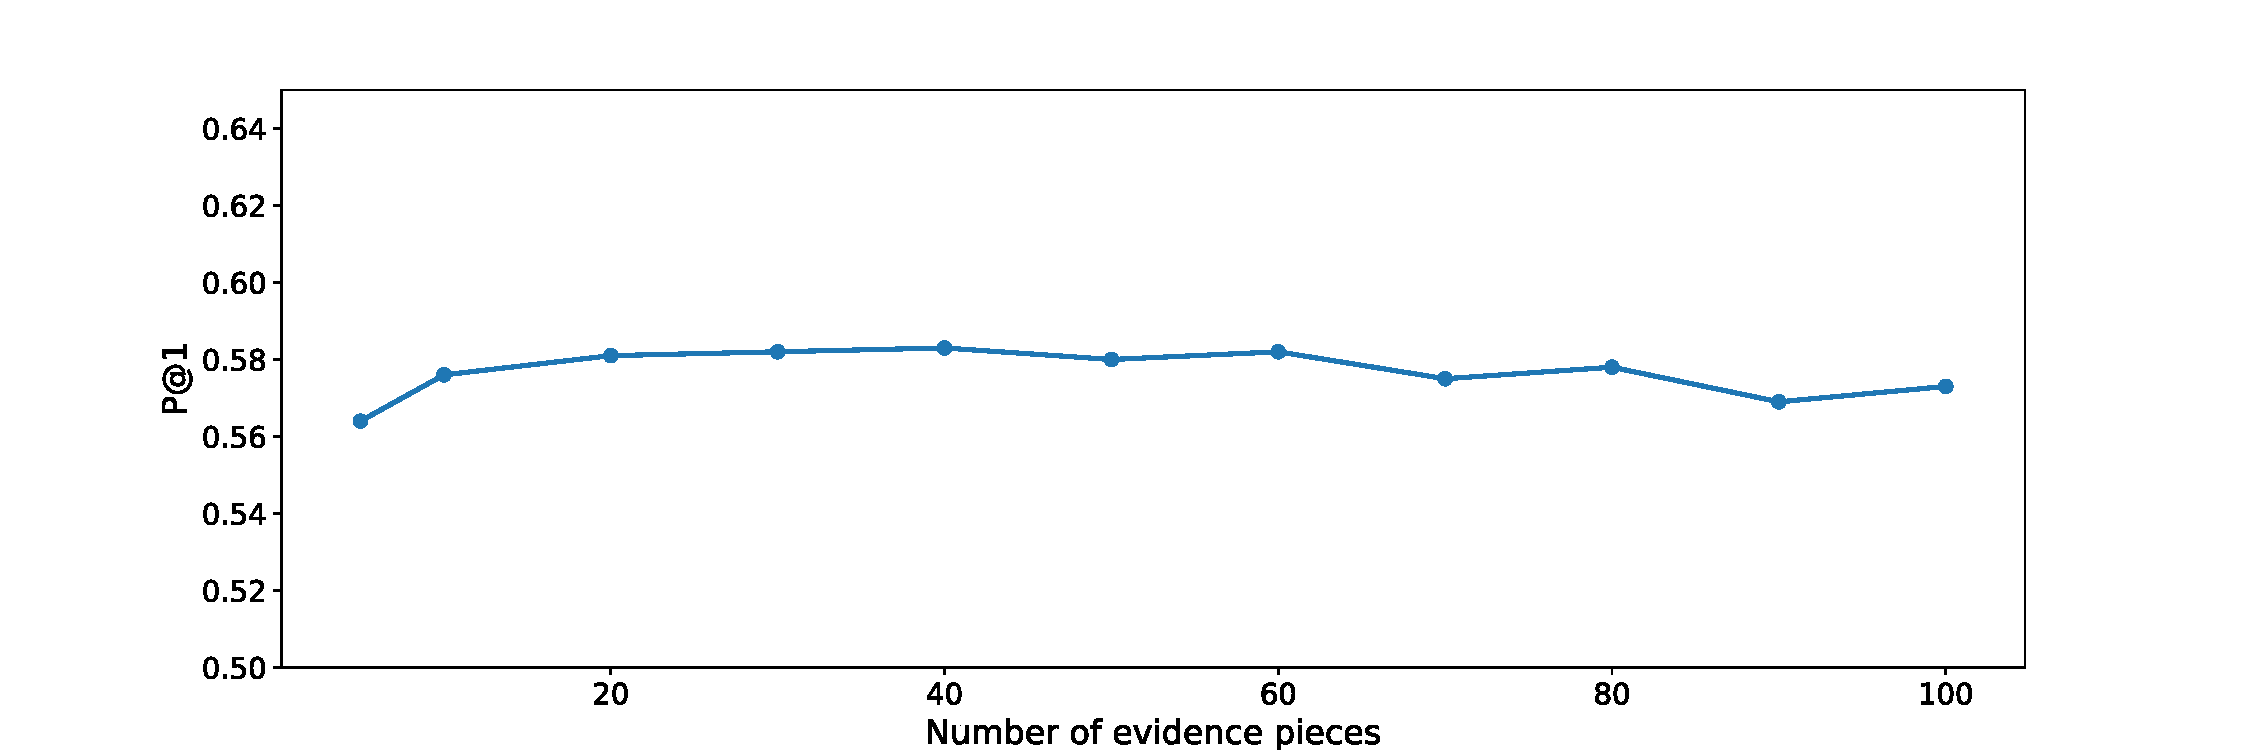
\includegraphics[width=0.8\textwidth]{submissions/Gerhard2024/figures/p_at_1-line_with_evidences.pdf}
    \vspace*{-0.2cm}
    \caption{Performance of \method on the \compmix dev set with different numbers of evidence.}
    \label{fig:res-num-evidences}
    \vspace*{-0.2cm}
\end{figure}



%%% ABLATION
\myparagraph{Ablation study on re-ranking} For more insight on the possible configurations of the RF stage, we conducted an ablation study with different options, including solely relying on the initial BM25 scoring without explicit re-ranking. The results are shown in Table \ref{tab:ablation2}. We observe that the iterative reduction in two steps is slightly better than the single-step variants (going down from top-1000 to top-30 in one RF step). Between the two options of using a GNN or a CE, the differences are negligible. A notable effect is that our RF techniques retain the answer presence at a very high level, only a bit lower than for the initial top-1000. 
The last two rows of Table \ref{tab:ablation2} demonstrate that RF is crucial: without explicit re-ranking, the technique of just picking smaller top-$k$ from the original BM25 model leads to substantial degradation in both answer presence and precision. 


\begin{table} [t] \small
    \centering
    \newcolumntype{G}{>{\columncolor [gray] {0.90}}c}
    \newcolumntype{H}{>{\setbox0=\hbox\bgroup}c<{\egroup}@{}}
    	\begin{tabular}{l G H G G G} 
        \toprule
            & \multicolumn{5}{G}{\textbf{\compmix} (dev set)} \\
        \midrule
            \textbf{RF Method $\downarrow$ / Metric $\rightarrow$} & \textbf{P@1} & \textbf{AP@1000} & \textbf{AP@100}  & \textbf{AP@30} & \textbf{MRR@100} \\ 
        \midrule
            \textbf{GNN: 1000 $\rightarrow$ 100 $\rightarrow$ 30}             &  $\mathbf{0.574}$  & $0.760$ &  $0.738$  &  $0.710$  &  $\mathbf{0.572}$  \\
            \textbf{CE: 1000 $\rightarrow$ 100 $\rightarrow$ 30}          &  $0.573$  & $0.760$  &   $\mathbf{0.740}$ &  $\mathbf{0.721}$   &  $0.553$   \\
        \midrule
            \textbf{GNN: 1000 $\rightarrow$ 30} &  $0.567$  & $?$  &   $n/a$ &  $0.710$   &  $0.567$   \\
         \textbf{CE: 1000 $\rightarrow$ 30} &  $0.570$  & $0.760$  &   $n/a$ &  $0.715$   &  $0.558$   \\
            \midrule
           \textbf{BM25: 100 (w/o GNN or CE)} &  $0.490$ & $0.760$  &  $0.652$  &  $n/a$  &  $0.259$ \\       
            \textbf{BM25: 30 (w/o GNN or CE)} &  $0.468$  & $0.760$  &  $n/a$ &  $0.534$   &  $0.259$   \\
            \bottomrule
    \end{tabular}
    \vspace*{-0.2cm}
    \caption{Ablation study for different RF strategies of \method on the \compmix dev set. The answer presence in the RF input with top-$1000$ evidence pieces is $0.760$.}
    \label{tab:ablation2}
\end{table}



\myparagraph{Quality of SI}
To assess the quality and robustness of the Structured Intents, we
inspected a sample of questions and their SIs.
Table~\ref{tab:question-SI-examples} gives three anecdotic examples.
We show SIs generated by \method, which makes use of the pre-existing collection from the \compmix benchmark for training.
This training data was obtained via different heuristics, 
which can be a limiting factor when user intents become more complex.

Therefore, we also looked at SIs derived via in-context learning (ICL) using \gptfour with $5$ handcrafted examples.
As shown in our earlier work on temporal QA~\cite{Jia-FAITH:WWW2024},
such data can be used for training smaller models (e.g., BART),
which can greatly boost the completeness and overall quality of the generated SIs.

From the sampled set, we observed that the ICL-based SIs are more
complete with all slots filled, whereas the BART-based SIs focused more
on the main slots Answer-type, Entities and Relation.
However, both approaches achieve very high quality in filling the slots,
capturing the user's information need very well.

Interestingly, when questions get complicated, with nested phrases, 
the ICL-based variant succeeds in decomposing the questions, based on only $5$ ICL examples.
For example, for the question {\em ``which German state had the most Corona-related death cases in the first year after the outbreak?''}
the Time slot becomes {\em ``first year after Corona outbreak''},
which can be resolved to identify the temporal scope.
In general, we believe that such question decomposition, beyond simple temporal constraints,
would be an interesting theme for future work.

\begin{table} [t] 
    \centering
    \small
    \newcolumntype{G}{>{\columncolor [gray] {0.90}}c}
    \newcolumntype{H}{>{\setbox0=\hbox\bgroup}c<{\egroup}@{}}
    \resizebox*{\textwidth}{!}{
        \begin{tabular}{p{6cm}|p{6cm}|p{6cm}} 
        \toprule
            \textbf{Question} & \textbf{Current SI by \method} & \textbf{SI via ICL} \\
        \midrule
        \textit{what was disneys first color movie?}
            & Ans-Type: \textit{animated feature film} & Ans-Type: \textit{film, animated film} \\
            & Entities: \textit{disneys} & Entities: \textit{Disney} \\
            & Relation: \textit{was first color movie} & Relation: \textit{first color movie} \\
            &  & Time: \textit{first} \\
        \midrule
        \textit{at the oscars, who won best actor in 2018?}
            & Ans-Type: \textit{human} & Ans-Type: \textit{person, actor} \\
            & Entities: \textit{at the oscars} & Entities: \textit{Oscars, 2018} \\
            & Relation: \textit{who won best actor in 2018} & Relation: \textit{won best actor} \\
            &  & Time: \textit{2018} \\
        \midrule
        \textit{which German state had the most Corona-} & Ans-Type: \textit{state} & Ans-Type: \textit{location, state} \\
        \textit{related death cases in the first year after} & Entities: \textit{Germany, Corona} & Entities: \textit{Germany, Corona-related deaths} \\
        \textit{the outbreak?} & Relation: \textit{which state had the most related} & Relation: \textit{highest count of death cases} \\
        & \textit{death cases in the first year after the out-}  & Location: \textit{Germany} \\
            & \textit{break}  & Time: \textit{first year after Corona outbreak} \\
        \bottomrule
    \end{tabular}
    }
    \vspace*{-0.2cm}
    \caption{Examples for pairs of question and generated SI.}
    \label{tab:question-SI-examples}
\end{table}




%%% REFRAIN FROM ANSWER
\myparagraph{Refraining from answering}
%%% Searched for: "generated_answer I" (with I being the full word, not partial) in the generated answers of LLaMA
%%% yields 245 results out of 2764 questions on CompMix
%%% yields 1270 results out of 3237 questions on TimeQuestions
We can train our model to refrain from answering in scenarios
where the provided evidence does not contain an answer to the question.
Specifically, during training, when the answer is not present in the evidence,
we change the target answer to {\em unknown}. This variant is referred to as \method {\em (faithful)}.

We measure the ratio of questions for which {\em unknown} is provided as answer,
and the P@1 restricted to questions that are answered.
The accuracy of refraining from answering is measured as well,
based on whether the answer is present in the evidence or not.
We conduct this experiment on \compmix and \timequestions,
for which we can compute answer presence exactly.
We also compute results for \llama, which is already instructed 
with the option to answer ``don't know''.
Table~\ref{tab:refrain-from-answer} shows the results.
For \compmix, we observe that \method has high accuracy on refraining when appropriate,
whereas \llama tends to be overconfident with a very small rate of {\em unknowns}, leading to incorrect answers.

\begin{table} [t] \small
    \centering
    \newcolumntype{G}{>{\columncolor [gray] {0.90}}c}
    \newcolumntype{H}{>{\setbox0=\hbox\bgroup}c<{\egroup}@{}}
    	\begin{tabular}{l G G G G c c c c} 
        \toprule
            & \multicolumn{4}{G}{\textbf{\compmix}} & \multicolumn{4}{c}{\textbf{\timequestions}} \\
            \midrule
            \textbf{Metric $\rightarrow$} & \textbf{P@1}  & \textbf{P@1} & \textbf{Refrain} & \textbf{Refrain} & \textbf{P@1}  & \textbf{P@1} & \textbf{Refrain} & \textbf{Refrain} \\ 
            \textbf{Method $\downarrow$} &                 & \textbf{(answered)} & \textbf{rate} & \textbf{accuracy} &                 & \textbf{(answered)} & \textbf{rate} & \textbf{accuracy} \\ 
            \midrule
                \textbf{\llama}             &  $0.431$  &  $0.471$  &  $0.089$  &  $n/a$  &  $0.177$  &  $0.276$  &  $0.392$  &  $n/a$  \\
                \textbf{\method (faithful)}           &  $0.497$  &  $0.713$  &  $0.303$  &  $0.838$ &  $0.597$  &  $0.804$  &  $0.257$  &  $0.864$  \\
            \bottomrule
    \end{tabular}
    \vspace*{-0.2cm}
    \caption{
        Performance of \method with option to refrain from answering (``don't know'').
    }
    \label{tab:refrain-from-answer}
\end{table}

\label{sec:disc}
\section{Insights, Limitations, and Challenges}


\noindent{\bf Benchmark Performance.} Our method, RAG-based \method with an 8B LLaMA model, outperforms much larger LLMs like \gptfour on two of the three benchmarks, with a very large margin for temporal questions. Obviously, pre-trained LLMs have only limited sense of properly positioning ``remembered’’ facts on the timeline even with training data that exceeds ours by several orders of magnitude. This confirms our intuition that LLMs alone are not good at ``recalling’’  higher-arity relations that require combining distant pieces of evidence. This is a sweet spot for RAG. Only for 
the \crag benchmark, \method is substantially inferior to a full-blown LLM. This is likely due to the nature of the questions: not necessarily the complexity of the information needs, but the need for more web sources (beyond what our experiments tap into).

\vspace{0.2cm}
\noindent{\bf Cost/Performance Ratio.} The most important take-away from our experiments is that \method achieves its competitive performance at a much lower cost than the full LLMs. Assuming that the consumed GFlops are proportional to the number of model parameters, \method achieves a cost reduction by a factor of 200x for \gptthree and 2000x for \gptfour. This does not only mean less computation, but also a massively lower electricity bill and climate impact.  

\vspace{0.2cm}
\noindent{\bf Role of Question Understanding.} We did not systematically investigate the influence of the Structured Intent in the \method pipeline. However, the comparison to the big GPT models reflects the role of the SI, as we prompt the GPT models in their natural mode with the original questions. The linearized sequence of available SI slots does not always have major advantages, but there are enough cases where specific facets provide crucial cues. This holds especially for the Entities slot, as this drives the gathering of evidence in the ER stage (cf.~\cite{Christmann-CONVINSE:SIGIR2022}, and for the Time slot, as these cues are often decisive for temporal questions (cf.~\cite{Jia-FAITH:WWW2024}).

\vspace{0.2cm}
\noindent{\bf Role of Re-Ranking.} As our ablation studies show, merely using top-$k$ evidence from an initial BM25-style ranking does not provide good performance. Also, there seems to be sweet spot in the choice of $k$: we need enough evidence for connecting the dots if the question requires multiple pieces of information, or for corroborating candidates if the question finds many useful but noisy pieces. In the experiments, $k=30$ turns out to be good choice; much lower $k$ results in insufficient evidence, and much larger $k$ leads to saturation and ultimately degrading performance. Our argument for iteratively shrinking the candidate set in multiple rounds of re-ranking is substantiated in our experiments, but the gain of doing this, compared to GNN- or CE-based re-ranking from 1000 to 30, is not big. More research is called to better understand the role of ranking in RAG. 

\vspace{0.2cm}
\noindent{\bf Limitations of Evidence Retrieval.}
For ER, we adopted more or less standard techniques. The results showed very good answer presence, in the order of 75\% in the top-100 or even top-30. An important case where this is insufficient are questions that require aggregating information over a large number of evidence pieces. An example is asking for the life-time total of 3-point scores of the basketball player Dirk Nowitzki.
This requires collecting a set of per-season tables with NBA player statistics, but also other web sources with numbers for his career before he joined the NBA (including his youth teams).
Of course, there are sometimes shortcuts like a Wikipedia article or biography mentioning the total number, but this cannot be universally assumed. The bottom line is that ER should be reconsidered as well, striving to improve the recall dimension.

\vspace{0.2cm}
\noindent{\bf Limitations of Answer Generation.}
For AG, we simply rely on a LLM,
using it as an extractor (``reader'') from the given evidence. Despite the wide belief that LLMs can perform deep
reasoning over many pieces of evidence, our experience is that the extraction works only well – robustly and faithfully – for relatively simple questions with a few multi-hop joins or simple aggregation over a few pieces. However, complicated questions such as asking for the top-100 NBA players with the largest number of life-time 3-point scores (again including their pre-NBA careers) are currently out of scope and will likely remain so for quite some time. This offers many opportunities for pushing the envelope further.

\vspace{0.2cm}
\noindent{\bf Trust in Data Sources.}
In our experiments, we considered all heterogeneous sources as trustworthy and unbiased. With focus on Wikidata and Wikipedia, this assumption has been well justified. In the wild, however, input data for RAG-based systems likely exhibit a wide spectrum of quality issues, in terms of stale information, biased positions, or simply false statements. Identifying trustworthy and up-to-date evidence and dealing with conflicting data, has been explored in other contexts (e.g., for KG curation~\cite{Dong-Trust:PVLDB2015}), but remains a major challenge for RAG-based QA.


\vspace{0.2cm}
\noindent{\bf Open Challenges and Future Work.} The best-performing methods in our experiment, mostly \method, reach P@1 values of 56\% for \compmix and 75\% for \timequestions. 
For the latter, the answer presence in the top-100 is only slightly higher; so the AG stage hardly misses anything.
However, for \compmix, the answer presence is 75\% -- much higher than what our system can actually answer. Obviously, closing this gap is a major direction to pursue, with focus on the RF and AG stages. However, missing one fourth of the answers completely in the top-100 pool, is a big problem as well. This requires improving recall at the ER stage, possibly with better guidance by the QU, which in turn needs more sources beyond the scope of our experiments (currently limited to Wikidata and Wikipedia). 

In general, we need to think beyond this kind of ``benchmark mindset’’. Even if we reached 80\% or 90\% precision and recall, we would still have a substantial fraction of questions that are answered incorrectly
or not at all. 
The remaining errors may not be a problem for chatbots, but they would be a showstopper for the deployment of mission-critical applications in business or science. We believe that this big gap is a shortcoming of {\em all methods}, not an issue that comes from the data alone. For trivia-style QA, as looked at in this paper, a smart human in ``open book’’ mode and no time limitation should be able to properly answer practically all questions, just by reading pieces of web contents and putting things together. Neither LLMs nor state-of-the-art RAG are the final solution; substantial research and creative ideas are needed to further advance QA.


\clearpage
\newpage

\newcommand{\bibauthors}[1]{{#1}}
\newcommand{\bibtitle}[1]{\emph{#1}}
\newcommand{\bibconf}[1]{{#1}}

\begin{thebibliography}{10}

\bibitem{Bajaj:arxiv2018}
\bibauthors{Payal Bajaj, Daniel Campos, Nick Craswell, Li Deng, Jianfeng Gao, Xiaodong Liu, Rangan Majumder, Andrew McNamara, Bhaskar Mitra, Tri Nguyen, Mir Rosenberg, Xia Song, Alina Stoica, Saurabh Tiwary, Tong Wang.}
\bibtitle{MS MARCO: A Human Generated MAchine Reading COmprehension Dataset.}
In \bibconf{arXiv 2018}.

\bibitem{DBLP:conf/acl/ChenFWB17}
\bibauthors{Danqi Chen, Adam Fisch, Jason Weston and Antoine Bordes.}
\bibtitle{Reading Wikipedia to Answer Open-Domain Questions.}
In \bibconf{ACL 2017}.

\bibitem{Christmann-CONVINSE:SIGIR2022}
\bibauthors{Philipp Christmann, Rishiraj Saha Roy, Gerhard Weikum.}
\bibtitle{Conversational Question Answering on Heterogeneous Sources.}
In \bibconf{SIGIR 2022}.

\bibitem{Christmann-CLOCQ:WSDM2022}
\bibauthors{Philipp Christmann, Rishiraj Saha Roy, Gerhard Weikum.}
\bibtitle{Beyond NED: Fast and Effective Search Space Reduction for Complex Question Answering over Knowledge Bases.}
In \bibconf{WSDM 2022}.

\bibitem{Christmann-Explaignn:SIGIR2023}
\bibauthors{Philipp Christmann, Rishiraj Saha Roy, Gerhard Weikum.}
\bibtitle{Explainable Conversational Question Answering over Heterogeneous Sources via Iterative Graph Neural Networks.}
In \bibconf{SIGIR 2023}.

\bibitem{Christmann-CompMix:WWW2024}
\bibauthors{Philipp Christmann, Rishiraj Saha Roy, Gerhard Weikum.}
\bibtitle{CompMix: A Benchmark for Heterogeneous Question Answering.}
In \bibconf{WWW 2024}.

\bibitem{Dejean:arxiv2024}
\bibauthors{Herve Dejean, Stephane Clinchant, Thibault Formal.}
\bibtitle{A Thorough Comparison of Cross-Encoders and LLMs for Reranking SPLADE.}
In \bibconf{arXiv 2024}.

\bibitem{Dhingra-time-aware-LLM:TACL2022}
\bibauthors{Bhuwan Dhingra, Jeremy R Cole, Julian Martin Eisenschlos, Daniel Gillick, Jacob Eisenstein, and William W Cohen.}
\bibtitle{Time-Aware Language Models as Temporal Knowledge Bases.}
In \bibconf{TACL 2022}.

\bibitem{Dong-Trust:PVLDB2015}
\bibauthors{Xin Luna Dong, Evgeniy Gabrilovich, Kevin Murphy, Van Dang, Wilko Horn, Camillo Lugaresi, Shaohua Sun, Wei Zhang.}
\bibtitle{Knowledge-Based Trust: Estimating the Trustworthiness of Web Sources.}
In \bibconf{PVLDB 2015}.

\bibitem{DBLP:journals/arXiv/abs-2312-10997}
\bibauthors{Yunfan Gao, Yun Xiong, Xinyu Gao, Kangxiang Jia, Jinliu Pan, Yuxi Bi, Yi Dai, Jiawei Sun, Qianyu Guo, Meng Wang, Haofen Wang.}
\bibtitle{Retrieval-Augmented Generation for Large Language Models: A Survey.}
In \bibconf{arXiv 2023}.

\bibitem{Gao-citations:emnlp2023}
\bibauthors{Tianyu Gao, Howard Yen, Jiatong Yu, Danqi Chen.}
\bibtitle{Enabling Large Language Models to Generate Text with Citations.}
In \bibconf{EMNLP 2023}.

\bibitem{Guu-REALM:ICML2020}
\bibauthors{Kelvin Guu, Kenton Lee, Zora Tung, Panupong Pasupat, Ming-Wei Chang.}
\bibtitle{Retrieval Augmented Language Model Pre-Training.}
In \bibconf{ICML 2020}.

\bibitem{DBLP:conf/eacl/IzacardG21}
\bibauthors{Gautier Izacard, Edouard Grave.}
\bibtitle{Leveraging Passage Retrieval with Generative Models for Open Domain Question Answering.}
In \bibconf{EACL 2021}.

\bibitem{Jia-TimeQuestions}
\bibauthors{Zhen Jia, Soumajit Pramanik, Rishiraj Saha Roy, and Gerhard Weikum.}
\bibtitle{Complex Temporal Question Answering on Knowledge Graphs.}
In \bibconf{CIKM 2021}.

\bibitem{Jia-FAITH:WWW2024}
\bibauthors{Zhen Jia, Philipp Christmann, Gerhard Weikum.}
\bibtitle{Faithful Temporal Question Answering over Heterogeneous Sources.}
In \bibconf{WWW 2024}.

\bibitem{DBLP:journals/arXiv/abs-2305-06984}
\bibauthors{Ehsan Kamalloo, Nouha Dziri, Charles L. A. Clarke, Davood Rafiei.}
\bibtitle{Evaluating Open-Domain Question Answering in the Era of Large Language Models.}
In \bibconf{arXiv 2023}.

\bibitem{Kandpal:ICML2023}
\bibauthors{Nikhil Kandpal, Haikang Deng, Adam Roberts, Eric Wallace, Colin Raffel.}
\bibtitle{Large Language Models Struggle to Learn Long-Tail Knowledge.}
In \bibconf{ICML 2023}.

\bibitem{DBLP:conf/emnlp/KarpukhinOMLWEC20}
\bibauthors{Vladimir Karpukhin, Barlas Oguz, Sewon Min, Patrick S. H. Lewis, Ledell Wu, Sergey Edunov, Danqi Chen, Wen-tau Yih.}
\bibtitle{Dense Passage Retrieval for Open-Domain Question Answering.}
In \bibconf{EMNLP 2020}.

\bibitem{Lee-MATTER:ACL2024}
\bibauthors{Dongkyu Lee, Chandana Satya Prakash, Jack FitzGerald, Jens Lehmann.}
\bibtitle{MATTER: Memory-Augmented Transformer Using Heterogeneous Knowledge Sources.}
In \bibconf{ACL 2024}.

\bibitem{DBLP:conf/acl/LewisLGGMLSZ20}
\bibauthors{Mike Lewis, Yinhan Liu, Naman Goyal, Marjan Ghazvininejad, Abdelrahman Mohamed, Omer Levy, Veselin Stoyanov, Luke Zettlemoyer.}
\bibtitle{BART: Denoising Sequence-to-Sequence Pre-training for Natural Language Generation, Translation, and Comprehension.}
In \bibconf{ACL 2020}.

\bibitem{DBLP:conf/nips/LewisPPPKGKLYR020}
\bibauthors{Patrick S. H. Lewis, Ethan Perez, Aleksandra Piktus, Fabio Petroni, Vladimir Karpukhin, Naman Goyal, Heinrich Küttler, Mike Lewis, Wen-tau Yih, Tim Rocktäschel, Sebastian Riedel, Douwe Kiela.}
\bibtitle{Retrieval-Augmented Generation for Knowledge-Intensive NLP Tasks.}
In \bibconf{NeurIPS 2020}.

\bibitem{Lin:MC2021}
\bibauthors{Jimmy Lin, Rodrigo Frassetto Nogueira, Andrew Yates.}
\bibtitle{Pretrained Transformers for Text Ranking: BERT and Beyond.}
In \bibconf{Morgan \& Claypool Publishers 2021}.

\bibitem{Liu-SUQL:NAACL2024}
\bibauthors{Shicheng Liu, Jialiang Xu, Wesley Tjangnaka, Sina J. Semnani, Chen Jie Yu, Monica Lam.}
\bibtitle{SUQL: Conversational Search over Structured and Unstructured Data with Large Language Models.}
In \bibconf{NAACL-HLT 2024}.

\bibitem{Mavi:FnT2024}
\bibauthors{Vaibhav Mavi, Anubhav Jangra, Adam Jatowt.}
\bibtitle{Multi-hop Question Answering.}
In \bibconf{Foundations and Trends in Information Retrieval 2024}.

\bibitem{Minaee-LLM-survey}
\bibauthors{Shervin Minaee, Tomas Mikolov, Narjes Nikzad, Meysam Chenaghlu, Richard}
\bibtitle{Socher, Xavier Amatriain, and Jianfeng Gao.}
Large Language Models: A Survey.
In \bibconf{arXiv 2024}.

\bibitem{Nogueira:arxiv2019}
\bibauthors{Rodrigo Frassetto Nogueira, Kyunghyun Cho.}
\bibtitle{Passage Re-ranking with BERT.}
In \bibconf{arXiv 2019}.

\bibitem{Oguz-UniK-QA:NAACL2022}
\bibauthors{Barlas Oguz, Xilun Chen, Vladimir Karpukhin, Stan Peshterliev, Dmytro Okhonko, Michael Sejr Schlichtkrull, Sonal Gupta, Yashar Mehdad, Scott Yih.}
\bibtitle{UniK-QA: Unified Representations of Structured and Unstructured Knowledge for Open-Domain Question Answering.}
In \bibconf{NAACL-HLT 2022}.

\bibitem{RogersGA:CS2023}
\bibauthors{Anna Rogers, Matt Gardner, Isabelle Augenstein.}
\bibtitle{QA Dataset Explosion: A Taxonomy of NLP Resources for Question Answering and Reading Comprehension.}
In \bibconf{ACM Computing Surveys 2023}.

\bibitem{RoyAnand:MC2021}
\bibauthors{Rishiraj Saha Roy, Avishek Anand.}
\bibtitle{Question Answering for the Curated Web: Tasks and Methods in QA over Knowledge Bases and Text Collections.}
In \bibconf{Synthesis Lectures on Information Concepts, Retrieval, and Services, Morgan \& Claypool Publishers 2021}.

\bibitem{Pramanik-Uniqorn:JWS2024}
\bibauthors{Soumajit Pramanik, Jesujoba Alabi, Rishiraj Saha Roy, Gerhard Weikum.}
\bibtitle{UNIQORN: Unified Question Answering over RDF Knowledge Graphs and Natural Language Text.}
In \bibconf{Journal of Web Semantics 2024}.

\bibitem{Sun-PullNet:EMNLP2019}
\bibauthors{Haitian Sun, Tania Bedrax-Weiss, William W. Cohen.}
\bibtitle{PullNet: Open Domain Question Answering with Iterative Retrieval on Knowledge Bases and Text.}
In \bibconf{EMNLP/IJCNLP 2019}.

\bibitem{Sun:NAACL2024}
\bibauthors{Kai Sun, Yifan Ethan Xu, Hanwen Zha, Yue Liu, Xin Luna Dong.}
\bibtitle{Head-to-Tail: How Knowledgeable are Large Language Models (LLMs)? A.K.A. Will LLMs Replace Knowledge Graphs?}
In \bibconf{NAACL-HLT 2024}.

\bibitem{Touvron-LLaMA}
\bibauthors{Hugo Touvron, Thibaut Lavril, Gautier Izacard, Xavier Martinet, Marie-Anne Lachaux, Timothée Lacroix, Baptiste Rozière, Naman Goyal, Eric Hambro, Faisal Azhar, Aurelien Rodriguez, Armand Joulin, Edouard Grave, Guillaume Lample.}
\bibtitle{Llama: Open and efficient foundation language models.}
In \bibconf{arXiv 2023}.

\bibitem{Wu-STARK:arxiv2024}
\bibauthors{Shirley Wu, Shiyu Zhao, Michihiro Yasunaga, Kexin Huang, Kaidi Cao, Qian Huang, Vassilis N. Ioannidis, Karthik Subbian, James Zou, Jure Leskovec.}
\bibtitle{STaRK: Benchmarking LLM Retrieval on Textual and Relational Knowledge Bases.}
In \bibconf{arXiv 2024}.

\bibitem{Wu:IEEE2021}
\bibauthors{Zonghan Wu, Shirui Pan, Fengwen Chen, Guodong Long, Chengqi Zhang, Philip S. Yu.}
\bibtitle{A Comprehensive Survey on Graph Neural Networks.}
In \bibconf{IEEE Transactions on Neural Networks and Learning Systems 2021}.

\bibitem{Yang-CRAG}
\bibauthors{Xiao Yang, Kai Sun, Hao Xin, Yushi Sun, Nikita Bhalla, Xiangsen Chen, Sajal Choudhary, Rongze D. Gui, Ziran W. Jiang, Ziyu Jiang, Lingkun Kong, Brian Moran, Jiaqi Wang, Yifan Ethan Xu, An Yan, Chenyu Yang, Eting Yuan, Hanwen Zha, Nan Tang, Lei Chen, Nicolas Scheffer, Yue Liu, Nirav Shah, Rakesh Wanga, Anuj Kumar, Wen-tau Yih, Xin Luna Dong.}
\bibtitle{CRAG -- Comprehensive RAG Benchmark.}
In \bibconf{arXiv 2024}.

\bibitem{Yasunaga:NAACL2021}
\bibauthors{Michihiro Yasunaga, Hongyu Ren, Antoine Bosselut, Percy Liang, Jure Leskovec.}
\bibtitle{QA-GNN: Reasoning with Language Models and Knowledge Graphs for Question Answering.}
In \bibconf{NAACL-HLT 2021}.

\bibitem{Zhang-Spaghetti:ACL2024}
\bibauthors{Heidi C. Zhang, Sina J. Semnani, Farhad Ghassemi, Jialiang Xu, Shicheng Liu, Monica S. Lam.}
\bibtitle{SPAGHETTI: Open-Domain Question Answering from Heterogeneous Data Sources with Retrieval and Semantic Parsing.}
In \bibconf{ACL 2024}.

\bibitem{Zhang:NAACL2024}
\bibauthors{Jiahao Zhang, Haiyang Zhang, Dongmei Zhang, Yong Liu, Shen Huang.}
\bibtitle{End-to-End Beam Retrieval for Multi-Hop Question Answering.}
In \bibconf{NAACL-HLT 2024}.

\bibitem{Zhao-LLMsurvey}
\bibauthors{Wayne Xin Zhao, Kun Zhou, Junyi Li, Tianyi Tang, Xiaolei Wang, Yupeng Hou, Yingqian Min, Beichen Zhang, Junjie Zhang, Zican Dong, Yifan Du, Chen Yang, Yushuo Chen, Zhipeng Chen, Jinhao Jiang, Ruiyang Ren, Yifan Li, Xinyu Tang, Zikang Liu, Peiyu Liu, Jian-Yun Nie, Ji-Rong Wen.}
\bibtitle{A Survey of Large Language Models.}
In \bibconf{arXiv 2023}.

\bibitem{Zhao:arxiv2024}
\bibauthors{Penghao Zhao, Hailin Zhang, Qinhan Yu, Zhengren Wang, Yunteng Geng, Fangcheng Fu, Ling Yang, Wentao Zhang, Bin Cui.}
\bibtitle{Retrieval-Augmented Generation for AI-Generated Content: A Survey.}
In \bibconf{arXiv 2024}.

\bibitem{Zhu-ODQA-survey:arxiv2021}
\bibauthors{Fengbin Zhu, Wenqiang Lei, Chao Wang, Jianming Zheng, Soujanya Poria, Tat-Seng Chua.}
\bibtitle{Retrieving and Reading: A Comprehensive Survey on Open-domain Question Answering.}
In \bibconf{arXiv 2021}.

\end{thebibliography}


\end{document}

    \end{opinion}
\end{opinionsection}

\begin{articlesection}{Personal Information Management}
%
%  Contributed articles section.  Use the articlesection environment.
%  Each article is contained in an article environment, where the two required
%  options to \begin{article} are the title and author of the article
%
\begin{article}
{Lifelogging As An Extreme Form of Personal Information Management - What Lessons To Learn}
{Ly-Duyen Tran, Cathal Gurrin, Alan F. Smeaton}
\setcounter{section}{0}
\documentclass{article}

\usepackage{deauthor}

\usepackage{latexsym}
\usepackage{graphicx}
\graphicspath{{./images/}}
\usepackage{booktabs} % for formal tables
\usepackage{color}  % for coloring text
\usepackage{amsmath}  % for aligning equations
\usepackage{subcaption}
\usepackage{caption}
\usepackage{tikz}
\usepackage{colortbl} % for color in tables
\usepackage{framed}
\usepackage{multirow}
\usepackage{multicol}
\usepackage{hyperref}
\usepackage{url}
\usepackage{balance}
\usepackage{verbatim}
\usepackage{cancel}
\usepackage{xspace} % for correcting space after macro commands
\usepackage{algorithm2e}
\usepackage{bbold} % for writing mathbb{1}
\usepackage{balance}
\usepackage{stmaryrd}
\usepackage{enumitem}
\usepackage{array} % package for hiding a column
\usepackage{bold-extra} % to enable textbf with textsc

% used for making text readable in document and .tex
% \setlength{\parindent}{0pt}

\newcommand{\struct}[1]{\texttt{\small #1}}
\newcommand{\utterance}[1]{\textit{#1}}
\newcommand{\phrase}[1]{\textit{``#1''}}

% \newcommand {\g}[1]{\textcolor[gray]{0.6}{#1}}

\newcommand{\drop}{\dag\xspace}

\newenvironment{Snugshade}[1][236,236,236]{
    \setlength{\itemsep}{0pt}
     \setlength{\parsep}{0pt}
     \setlength{\topsep}{0pt}
     \setlength{\partopsep}{0pt}
     \setlength{\leftmargin}{1.5em}
     \setlength{\labelwidth}{0em}
     \setlength{\labelsep}{0em} 
    \setlength{\parskip}{0pt}
    \definecolor{shadecolor}{RGB}{#1}
    \begin{snugshade}
}{
    \end{snugshade}
}


\newcommand{\method}{\textsc{Quasar}\xspace}
\newcommand{\benchmark}{\textsc{PerQA}\xspace}
\newcommand{\itemslist}[1]{$\langle$\struct{#1}$\rangle$}


\newcommand{\convinse}{\textsc{Convinse}\xspace}
\newcommand{\explaignn}{\textsc{Explaignn}\xspace}
\newcommand{\clocq}{\textsc{Clocq}\xspace}
\newcommand{\unikqa}{\textsc{UniK-Qa}\xspace}
\newcommand{\gptthree}{\textsc{Gpt-3}\xspace}
\newcommand{\gptfour}{\textsc{Gpt-4}\xspace}
\newcommand{\llama}{\textsc{Llama3}\xspace}
\newcommand{\spaghetti}{\textsc{Spaghetti}\xspace}


\newcommand{\compmix}{\textsc{CompMix}\xspace}
\newcommand{\timequestions}{\textsc{TimeQuestions}\xspace}
\newcommand{\crag}{\textsc{Crag}\xspace}


\newcommand{\squishlist}{
    \begin{list}{$\bullet$}{
        \setlength{\itemsep}{0pt}
	\setlength{\parsep}{3pt}
	\setlength{\topsep}{3pt}
	\setlength{\partopsep}{0pt}
	\setlength{\leftmargin}{1.5em}
	\setlength{\labelwidth}{1em}
	\setlength{\labelsep}{0.5em}
    }
}

\newcommand{\squishend}{
    \end{list}
}

\newcommand{\myparagraph}[1]{\vspace*{0.2cm}\noindent \textbf{#1}.}
\newcommand{\myparagraphnospace}[1]{\noindent \textbf{#1}.}

% \newcommand{\GW}[1]{\emph{{\color{blue} GW:#1}}}
% \newcommand{\PC}[1]{\emph{{\color{orange} PC: #1}}}
% \newcommand{\tocite}{{{\color{red} [CITE]}}}


\begin{document}

\title{RAG-based Question Answering \\ over Heterogeneous Data and Text}

\author{
Philipp Christmann,
Gerhard Weikum\\\\
Max Planck Institute for Informatics\\
Saarland Informatics Campus, Germany\\
\texttt{\{pchristm, weikum\}@mpi-inf.mpg.de}}

\maketitle

\section*{Abstract}
This article presents the \method system for question answering over unstructured text, structured tables, and knowledge graphs, with unified treatment of all sources.
The system adopts a RAG-based architecture, with a pipeline of evidence retrieval followed by answer generation, with the latter powered by a 
moderate-sized
language model.
Additionally and uniquely, \method
has components for question understanding, to derive crisper input for evidence retrieval, and for re-ranking and filtering the retrieved evidence before feeding the most informative pieces into the answer generation.
Experiments with three different benchmarks demonstrate the high answering quality of our approach, being on par with or better than large GPT models, while keeping the computational cost and energy consumption orders of magnitude lower.

\label{sec:intro}
\section{Introduction}

\noindent\textbf{Motivation and Problem.} The task of question answering, QA for short, arises in many flavors: factual vs. opinions, simple lookups vs. multi-hop inference, single answer vs. list of entities, 
direct answers vs. long-form, one-shot questions vs. conversations, and other varieties 
(see, e.g., surveys~\cite{RogersGA:CS2023,RoyAnand:MC2021}).
The state-of-the-art for this entire spectrum has been greatly advanced in the past decade. Most notably, incorporating deep learning into retriever-reader architectures (e.g.,~\cite{DBLP:conf/acl/ChenFWB17,DBLP:conf/eacl/IzacardG21,DBLP:conf/emnlp/KarpukhinOMLWEC20}) has boosted answering quality, and most recently, large language models (LLM)~\cite{Minaee-LLM-survey,Zhao-LLMsurvey} have pushed the envelope even further (e.g.,~\cite{DBLP:journals/arXiv/abs-2305-06984}).

% strengths and limitations of LLM for QA
Today’s LLMs alone are capable of accurately answering many \textit{factoid} questions, simply from their pre-trained parametric memory which latently encodes huge text corpora and other online contents.
However, this critically depends on the frequency of evidence in the underlying contents and the complexity of the information need. 
For example, 
asking for the {\em MVP of the 2024 NBA season} would easily return the correct answer Nikola Jokic, 
but asking for the {\em highest-scoring German NBA player} or the {\em MVP of the 2024 German basketball league} pose a big challenge.
The reason is that LLMs alone do not easily recall information about not so popular or even long-tail entities~\cite{Kandpal:ICML2023,Sun:NAACL2024},
and that they are mainly geared for direct look-ups as opposed to connecting multiple pieces of evidence~\cite{Mavi:FnT2024,Zhang:NAACL2024}.

% introduce RAG and discuss need for heterogeneous sources
\cite{DBLP:journals/arXiv/abs-2312-10997,Guu-REALM:ICML2020,DBLP:conf/nips/LewisPPPKGKLYR020,Zhao:arxiv2024}
known as RAG, address these bottlenecks. In addition to cleverly crafted prompts and few-shot examples, the LLM is provided with the top-ranked results of an explicit retrieval step, like web search or knowledge graph (KG) lookups. The former is often necessary for freshness of answers, and the latter may help with long-tail entities and also mitigate the notorious risk of hallucinations. Still, this generation’s RAG architectures are limited in how broad and how deep they tap into external sources. Popular AI assistants like Gemini or ChatGPT seem to primarily retrieve from the text of web pages (incl. Wikipedia articles), and academic research has additionally pursued knowledge augmentation by enhancing prompts with facts from large KGs (e.g., Wikidata).

An additional content modality that is still underexplored are {\em online tables}: a wide range of tabular data including HTML tables in web pages, spreadsheets and statistics, all the way to CSV and JSON datasets that are abundant on the Internet. There is prior work on joint support for text and KGs and for text and tables, but very little on all of these together -- some notable exceptions being~\cite{Christmann-CONVINSE:SIGIR2022,Christmann-Explaignn:SIGIR2023,Oguz-UniK-QA:NAACL2022,Zhang-Spaghetti:ACL2024}.


\noindent\textbf{Examples.} All three heterogeneous types of sources are crucial not only for answering different questions from different kinds of evidence, but also for combining multiple pieces of evidence of different modalities to infer correct and complete answers.
To 
illustrate
the need for tapping all sources, consider the following questions:

% \vspace*{0.2cm}
\begin{quote}
$Q1$: \utterance{Which Chinese basketballers have played in the NBA?}\\
 \indent $Q2$: \utterance{Who was the first Chinese NBA player?}\\
  \indent $Q3$: \utterance{Which Chinese NBA player has the most matches?}
\end{quote}
% \vspace*{0.2cm}

Q1 can be cast into querying a KG, but the list there is not necessarily complete and up-to-date, so additional evidence from text or tables would be desired. 
Q2 needs information about who played in which seasons, found only in web pages or sports-statistics tables. 
Finally, Q3 may be lucky in finding prominent textual evidence (e.g., in biographies, Wikipedia etc.), but this often faces divergent statements, and resolving contradictions needs to dive into more evidence. Besides, when textual evidence is rare and hard to find or not trustworthy enough, then information from multiple tables and text snippets may have to be aggregated (e.g., totals of per-season counts).
Some of this may perhaps become feasible for an industrial LLM’s RAG capabilities in the near future, but there are always harder scenarios by moving from Chinese NBA players deeper into the long tail, such as asking for {\em Lithuanian players in the German handball league}.

\vspace*{0.2cm}
\noindent\textbf{Approach and Contribution.} This paper presents a simple but powerful and versatile RAG system with unified access to text, KG and tables. We call our method {\em \method} 
(for Question Answering over Heterogeneous Sources with Augmented Retrieval).
Its architecture is relatively straightforward: all heterogeneous content is verbalized and indexed for retrieval; a retriever finds top-ranked results for the given question (from different source types), and these are fed into the LLM for answer generation. This is the unsurprising bird-eye’s view. Specific details that are key factors for the strong performance of \method are: 

\squishlist
\item[i)] automatically casting user questions into a structured representation of the information need, which is then used to guide 
\item[ii)] judicious ranking of search results, with multiple rounds of re-ranking and pruning, followed by
\item[iii)]	extracting faithful answers from an LLM in RAG mode, with answers grounded in tangible evidence.
\squishend


\vspace{0.2cm}
\noindent The paper presents experiments with three different benchmarks, covering various flavors of questions.
We focus on one-shot questions; conversational QA is out of scope here, but \method itself is well applicable to this case, too.
Our experiments demonstrate that our methods are competitive, on par with big GPT models and often better,
while being several orders of magnitude lower in computational and energy cost.
The experimental findings also highlight that question understanding, with structured representation of user intents, and iterative re-ranking of evidence are crucial for good performance.

Overall, our contribution lies in proposing a unified system architecture for RAG-based question answering over a suite of different data sources, with strong points regarding both effectiveness (i.e., answer quality)
and efficiency (i.e., computational cost).


\label{sec:background}
\section{Related Work}

The RAG paradigm came up as a principled way of enhancing LLM factuality incl. provenance and mitigating the risk of hallucination~\cite{Guu-REALM:ICML2020, DBLP:conf/nips/LewisPPPKGKLYR020}.
It is highly related to the earlier
retriever-reader architectures for QA~\cite{DBLP:conf/acl/ChenFWB17,DBLP:conf/emnlp/KarpukhinOMLWEC20}, especially when the reader uses the fusion-in-decoder method~\cite{DBLP:conf/eacl/IzacardG21,Oguz-UniK-QA:NAACL2022}.
Since its invention, RAG methodology has been greatly advanced, introducing a wide suite of extensions, such as batched inputs, interleaving retrieval and generation steps, and more (see the recent surveys~\cite{DBLP:journals/arXiv/abs-2312-10997,Zhao:arxiv2024}).

On question answering (QA), there is a vast amount of literature including a wealth of differently flavored benchmarks (see, e.g.,~\cite{RogersGA:CS2023}).
The case of interest here is QA over heterogeneous sources, tapping into both unstructured content and structured data. 
A variety of works has pursued this theme by combining knowledge graphs with text sources, using graph-based methods, neural learning and  language models (e.g.,~\cite{Pramanik-Uniqorn:JWS2024,Sun-PullNet:EMNLP2019,Yasunaga:NAACL2021}).

Most relevant for this article is the research on jointly leveraging all different sources: text, KGs, and tables (incl. CSV and JSON files). This includes  
the \unikqa system~\cite{Oguz-UniK-QA:NAACL2022},
the \spaghetti/SUQL project~\cite{Liu-SUQL:NAACL2024,Zhang-Spaghetti:ACL2024},
the \textsc{Matter} method~\cite{Lee-MATTER:ACL2024},
the STaRK benchmarking~\cite{Wu-STARK:arxiv2024},
and our own prior work
~\cite{Christmann-CONVINSE:SIGIR2022,Christmann-Explaignn:SIGIR2023} (without claiming exhaustiveness).
Out of these, we include \unikqa, \spaghetti and our own systems \convinse and \explaignn as baselines in the experimental evaluation.
Their architectures are similar to ours, but \unikqa and \spaghetti do not have our distinctive elements of
question understanding and iterative re-ranking (originally introduced in \explaignn~\cite{Christmann-Explaignn:SIGIR2023}).

\label{sec:method}
\section{Methodology}

\begin{figure}[tb]
  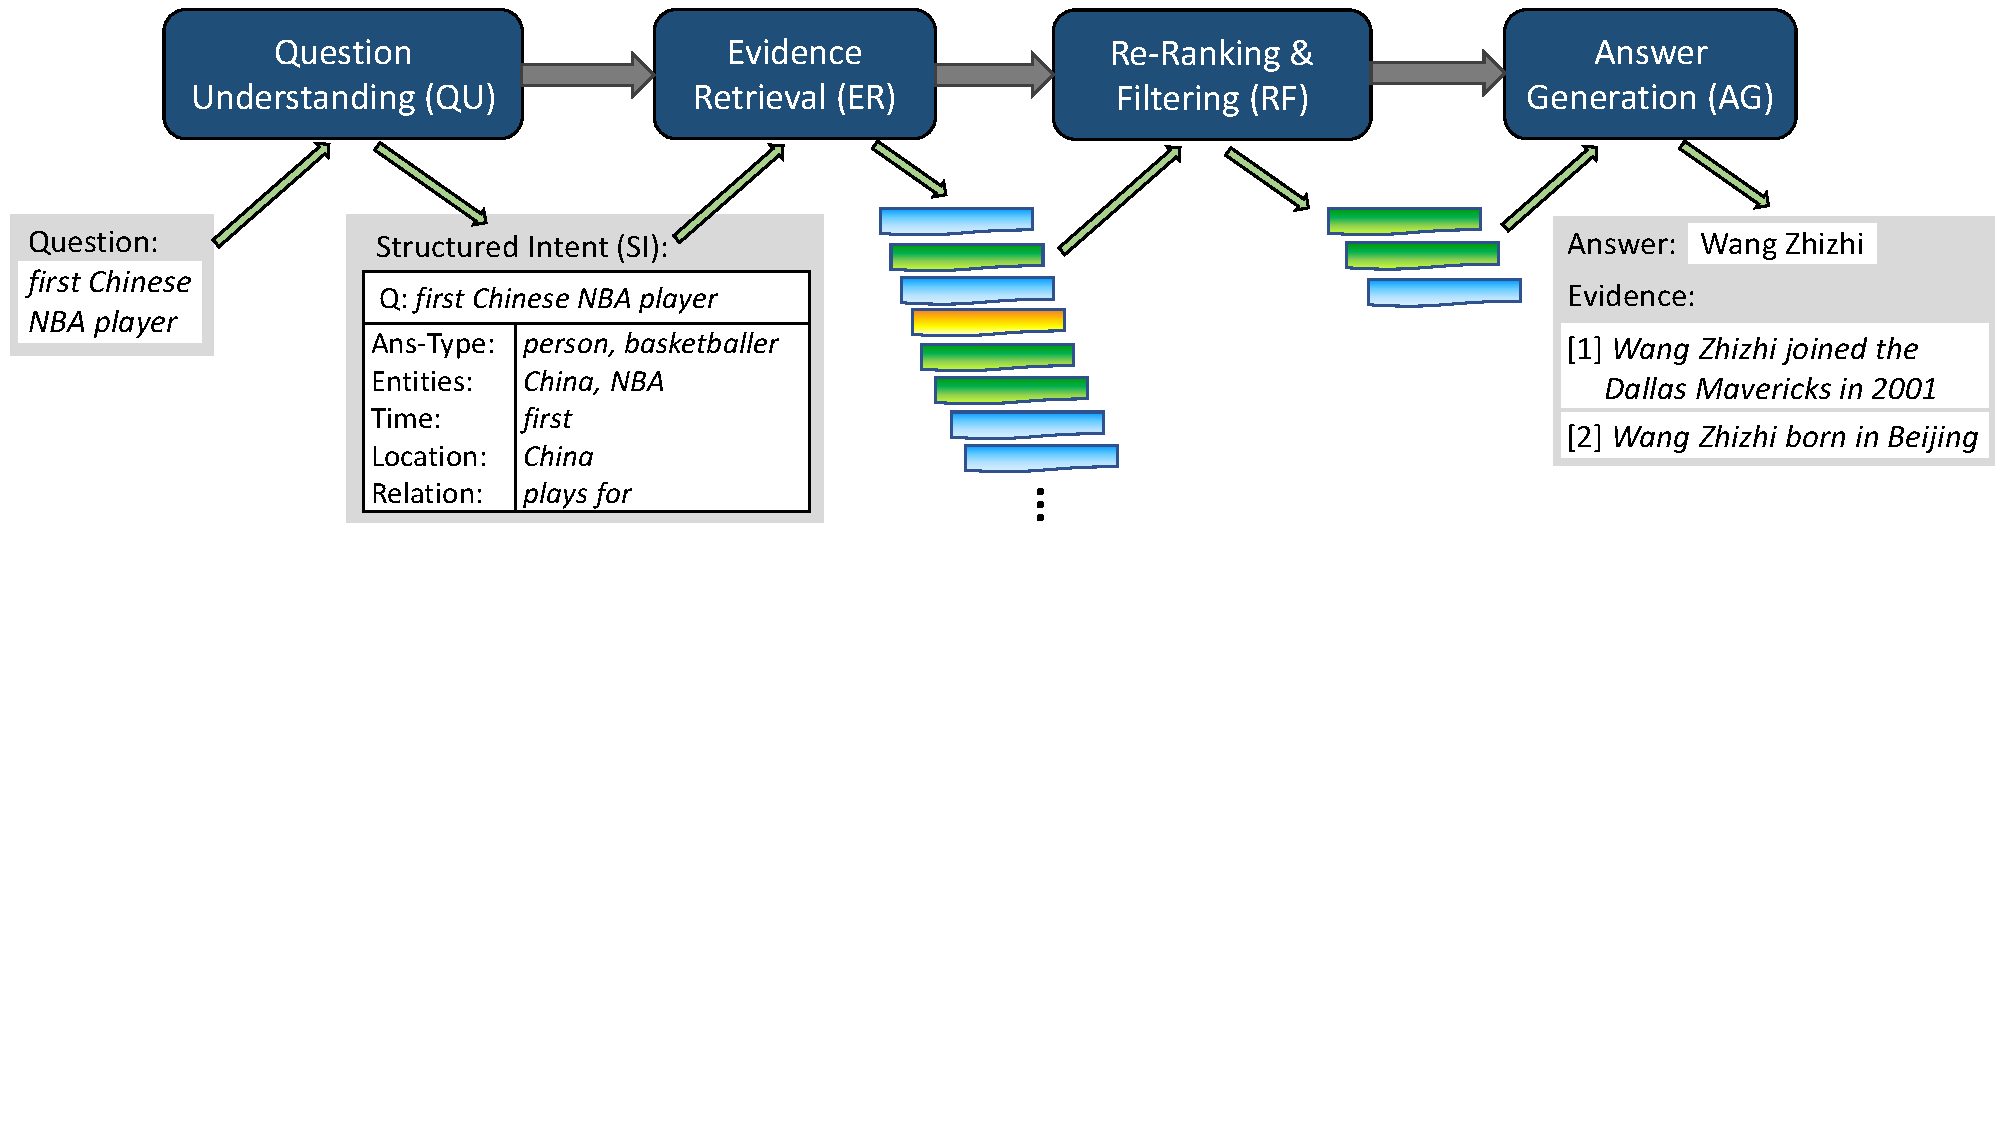
\includegraphics[width=\textwidth]{submissions/Gerhard2024/figures/compass-overview.pdf}
  \caption{Overview of the \method system.}
  \label{fig:compass-overview}
\end{figure}

% start with system overview
The \method system is a pipeline of four major stages, as illustrated in Figure \ref{fig:compass-overview}.
First, the input question is analyzed and decomposed, in order to compute a {\em structured intent (SI)} representation that will pass on to the subsequent steps, along with the original question. Second, the SI is utilized to retrieve pieces of evidence from different sources: text, KG and tables. 
Third, this pool of potentially useful evidence is filtered down, with iterative re-ranking, to arrive at a tractably small set of most promising evidence.
The final stage generates the answer from this evidence,
passing back the answer as well as evidence snippets for user-comprehensible explanation.

The second and fourth stage, Evidence Retrieval (ER) and Answer Generation (AG), are fairly standard. Such a two-phase architecture was called a retriever-reader architecture~\cite{Zhu-ODQA-survey:arxiv2021}. With a modern LLM replacing the earlier kinds of neural readers, this is the core of every RAG system~\cite{DBLP:journals/arXiv/abs-2312-10997}.

Stages 1 and 3 are unique elements of our architecture, judiciously introduced to improve both effectiveness (i.e., answer quality) and efficiency (i.e., computational cost).
Question Understanding (QU) provides the ER component with crisper and semantically refined input, and
the Re-Ranking \& Filtering (RF) stage is beneficial for
distilling the best evidence from the large pool of retrieved pieces.
The following subsections elaborate on the four stages of the pipeline, emphasizing the \method-specific steps QU and RF.



\subsection{Question Understanding (QU)}

% one par introducing the SI
To prepare the retrieval from different kinds of sources, including a KG, ad-hoc tables and text documents, it is useful to analyze and decompose the user question.
In this work, we aim to cast a question into a 
{\em structured intent (SI)} representation: essentially
a frame with faceted cues as slots, or equivalently, a concise set of key-value pairs. 
Figure \ref{fig:compass-overview} gives an idealized example for the question about the first Chinese NBA player. The facets or keys of potential interest here 
are:
\squishlist
\item {\em Ans-Type:} the expected answer type (or types when considering
different levels of semantic refinement), 
\item {\em Entities:} the salient entities in the question, and 
\item {\em Relation:} phrases that indicate which relation (between Q and A entities) the user is interested in. 
\squishend
\noindent In addition, as questions can have temporal or spatial aspects, the SI also foresees slots for:
\squishlist
\item {\em Time:} cues about answer-relevant time points or spans, including relative cues (e.g., ``before Covid'') and ordinal cues (e.g., ``first''), and
\item {\em Location:} cues about answer-relevant geo-locations.
\squishend

% discuss the spectrum of different SIs
\vspace{0.2cm}
\noindent The ideal SI for example question Q2 would look like:

\begin{quote}
{\em Ans-Type:} person, basketballer; {\em Entities:} China, NBA; {\em Time:} first;
{\em Location:} China; {\em Relation:} plays for.
\end{quote}

Note that the values for these slots can be crisp like entity names or dates, but they can also take the form of surface phrases. The SI purpose and value lie in the decomposition. In practice, many questions would only lead to a subset of faceted cues, leaving some slots empty. For the example in Figure \ref{fig:compass-overview}, an alternative SI could simply consist of

\begin{quote}
{\em Ans-Type:} person; {\em Entities:} China, NBA; {\em Time:} first.
\end{quote}

\noindent Even this simplified SI can be highly beneficial in guiding the subsequent evidence retrieval.

% sketch how an LM is trained to generate SIs 
To generate the SI from a user question, we employ a (small-scale) LM, specifically BART~\cite{DBLP:conf/acl/LewisLGGMLSZ20}, a Transformer-based auto-encoder with 140M parameters.\footnote{\url{https://huggingface.co/facebook/bart-base}}
BART is pre-trained for language representation; its power for our purpose comes from fine-tuning.
To this end, we generate (question, SI) pairs by using an instruction-trained LLM like GPT-4, with few-shot in-context learning (following our earlier work~\cite{Jia-FAITH:WWW2024}). 
Note that this is a one-time action; at inference-time we only use much smaller LMs.
The generated silver-standard pairs are then used to fine-tune BART.
In the experiments in this article, we leverage pre-existing collections of silver pairs, based on the training data of the CompMix benchmark~\cite{Christmann-CompMix:WWW2024}, 
comprising $3{,}400$ such pairs.


% outline value of SI for conversations
Although this paper focuses on single-shot questions, the \method architecture is also geared for conversational QA. In that setting, the SI can play an even bigger role, as (follow-up) questions are often formulated in a rather sloppy manner -- all but self-contained. For example, a conversation could start with a clear question {\em When did Wang Zhizhi join the NBA?}, followed a few dialog steps later, by a user utterance like {\em Which teams did he play for?} or simply {\em Which teams?}.
In such an informal conversation, the system needs to {\em contextualize} each user utterance based on the preceding turns in the dialog (e.g., inferring the relevant entities Wang Zhizhi and NBA from the conversational history).
For details on conversational QA, based on our architecture, see our earlier works~\cite{Christmann-CONVINSE:SIGIR2022,Christmann-Explaignn:SIGIR2023}.







%%%%%%%%%%%%%%%%%%%%%%%%%%%%%%%%%%%%%
\subsection{Evidence Retrieval (ER)}

The ER stage taps into a knowledge graph, a corpus of text documents, and a collection of web tables.
Specifically, for the experiments, we use the Wikidata KG,
all English Wikipedia articles, and all tables that are embedded in Wikipedia pages (incl. infoboxes, which can be seen as a special case of tables). 

% specifics: Clocq etc. - and the role of the SI
\vspace{0.2cm}
\noindent{\bf Retrieval from KG:}
To retrieve evidence from the KG, we utilize our earlier work
\clocq~\cite{Christmann-CLOCQ:WSDM2022}, which provides entity disambiguations and a relevant KG-subgraph for a given query.
Unlike most other works on QA-over-KG, \clocq fetches all KG-facts that are relevant for a given entity in a single step.
For example, when querying for
NBA players, it can traverse the KG neighborhood and pick up top teams, also considering so-called qualifier nodes in Wikidata which are often used for temporal scopes. 
As the disambiguation of entity names onto the KG can be tricky and noisy (e.g., China could be mapped to Chinese sports teams in all kinds of sports), \clocq considers several possible disambiguations~\cite{Christmann-CLOCQ:WSDM2022} (typically in the order of $10$ result entities).
The queries for \clocq are 
constructed by concatenating all slots of the question's SI.
For the example query about the first Chinese NBA player,
good result entities would be Dallas Mavericks, lists about NBA seasons, MVP awards etc., and their associated facts. These provide cues, but are likely insufficient to answer the question.


\vspace{0.2cm}
\noindent{\bf Retrieval from Text and Tables:}
The disambiguated entities returned by \clocq form anchors for tapping into text and tables.
\method first identifies 
relevant text documents and tables that refer to the anchor entities. With focus on Wikipedia, these are simply the articles for the respective entities. 
\method then constructs a keyword query that concatenates all available fields of the SI.
The query is evaluated against a linearized and verbalized representation (see below) of all sentences and all table rows in the selected documents.
This returns a set of sentences and 
and individual table rows, ranked by BM25 scores.


\vspace{0.2cm}
\noindent{\bf Evidence Verbalization:}
All results from the different data sources are uniformly treated by {\em linearizing} and {\em verbalizing} them
into token sequences. For KG results, the entity-centric triple sets are linearized via breadth-first traversal of the mini-graph starting from the entity node.
For tables, results are individual rows, which are contextualized by including labels from column headers and from the DOM-tree path of the article where the table comes from. For example, a table row about Wang Zhizhi playing for Dallas (Mavericks) in the 2000-2001 season, would be expressed as:

\vspace{0.05cm}
\hspace*{0.5cm} Wang Zhizhi / NBA Career / Season: 2000-2001, Team: Dallas, Games Played: 5 \dots
\vspace{0.05cm}

\noindent Finally, results from the text corpus are already in the form of token sequences, but we can additionally prefix these with the DOM-tree labels.
We can think of this entire pool of evidence as 
an on-the-fly corpus of potentially relevant pseudo-sentences, forming the input of the subsequent RF stage.


\vspace{0.2cm}
\noindent {\bf Result Ranking:}
Overall, the ER stage compiles a substantial set of evidence, possibly many thousands of entities, text snippets and table rows. Therefore, we practically restrict the pool to a subset of high-scoring pieces, like the top-$1000$.
For scoring, a simple BM25 model (a classical IR method) is applied. 
By default, we treat all evidence pieces uniformly with global scoring, no matter whether they come from KG, text or tables. 


\subsection{Re-Ranking and Filtering (RF)}

With a pool of top-$1000$ evidence pieces, we could invoke an LLM for answer generation. However, that would face a large fraction of noise (i.e., misleading evidence) and incur high costs of computation and energy consumption. 

For both of these reasons, we have devised light-weight techniques for iteratively reducing the top-$1000$ pieces to a small subset, say top-$30$ or top-$10$, that can be fed into an LLM at much lower cost (as LLM computations and pricing are at least linear in the number of input tokens). The difficulty is, of course, to do this without losing good evidence and reducing answer presence. Our techniques for this task are based on graph neural networks (GNNs)~\cite{Wu:IEEE2021} or cross-encoders (CEs)~\cite{Dejean:arxiv2024,Lin:MC2021}.

\myparagraph{GNN-based RF}
Given a large pool of evidence pieces from all sources, a bipartite graph is constructed:
\squishlist
\item {\em nodes} being evidence pieces or entities that occur in these pieces, and
\item {\em edges} connecting an evidence piece and an entity if the entity occurs in the evidence.
\squishend


The task for the GNN is to jointly score the evidence and the entity nodes in a multi-task learning setup. The latter are the {\em answer candidates}, and the evidence should give {\em faithful explanation} for an answer.
We build on our earlier work on explainable QA~\cite{Christmann-Explaignn:SIGIR2023}.

The node encodings are initialized with cross-encoder embeddings (see below) 
for node contents and the SI of the question. The inference iteratively adjusts the encodings based on message passing from neighboring nodes.
The GNN is trained via weak supervision from question-answer pairs:
evidence nodes are labeled as relevant if they are connected to
a gold answer.
More technical details are given in~\cite{Christmann-Explaignn:SIGIR2023}.

\method invokes the GNN in multiple rounds, iteratively reducing top-$k$ to top-$k^*$ nodes with $k^* \ll k$. In practice, we would typically consider two rounds: re-ranking top-$1000$ and pruning to top-100, and then reducing to top-30 or top-10, which are passed to the answer generation stage.
Note that this keeps the GNN at a tightly controlled size, so that its computational costs at inference-time are much smaller than those of an LLM.


\myparagraph{CE-based RF}
An alternative to the GNN inference is to employ a cross-encoder for scoring and re-ranking the evidence pieces.
These are transformers (typically with a small LM like BERT) that are fine-tuned for scoring the relatedness between a query and a document~\cite{Nogueira:arxiv2019}. In our case, the comparison is between the question SI and the evidence piece. In our experiments, we make use of two different cross-encoders, 
both trained on the MS-MARCO benchmark for passage retrieval~\cite{Bajaj:arxiv2018}, 
and fine-tuned on the respective benchmark (leveraging the same weak supervision data as for the GNNs),
the difference being in model size.\footnote{\url{https://huggingface.co/cross-encoder/ms-marco-MiniLM-L-4-v2} and\\ \url{https://huggingface.co/cross-encoder/ms-marco-MiniLM-L-6-v2}}
We use the smaller model to reduce top-$1000$ to top-100, and the larger model to go further down from top-100 to top-30.




%%%%%%%%%%%%%%%%%%%%%%%%%%%%%%%%%%%%%

\subsection{Answer Generation (AG)}

The last stage follows mainstream practice to invoke an LLM in a retrieval-augmented manner.
We call a `small-scale` LLM, specifically a fine-tuned LlaMA-3.1 model (8B-Instruct)\footnote{\url{https://huggingface.co/meta-llama/Llama-3.1-8B-Instruct}}, with a prompt \footnote{The specific prompt is \phrase{SI: \textless\texttt{concatenated SI}\textgreater \hspace{0.1cm} Evidence: \textless\texttt{evidence pieces}\textgreater}.}
consisting of:

\squishlist
\item the concatenated SI of the original question, and
\item the top-30 (or other top-$k^*$ with small $k^*$) evidence pieces.
\squishend

By the previous down-filtering of the original pool of evidence pieces, this last step has affordable cost in terms of computation time and energy consumption.

\vspace{0.2cm}
\noindent{\bf Fine-Tuning the LLM:}
We considered adding an instruction to the prompting, such as {\em ``answer this question solely based on the provided evidence snippets''}.
However, this turned out to be ineffective.
The reason why the model works well without such instructions is our task-specific fine-tuning.
We perform this by running the training data of benchmarks through the \method pipeline,
and training the AG stage with the top-30 evidence pieces as input.
Thus, the fine-tuning makes the model learn the role of evidence for RAG-based QA.

\vspace{0.2cm}
\noindent{\bf Explanations:}
The top-30 evidence pieces can be used to provide users with explanation of answers.
Optionally, these could be reduced further for comprehensibility.
Alternatively, we can fine-tune the LLM to provide both answers and concise explanations.
Since we can infer which evidences in the input mention the annotated ground-truth answers,
our method could be fine-tuned to provide such \textit{answering evidences} as well (cf.~\cite{Gao-citations:emnlp2023}).

\label{sec:exp}
\section{Experiments}


\label{setup}
\subsection{Experimental setup}


%%% BENCHMARKS
\myparagraphnospace{Benchmarks} We run experiments on three benchmarks with different characteristics of questions.

\squishlist
    \item \textbf{\compmix}.
    \compmix~\cite{Christmann-CompMix:WWW2024} is a benchmark which was specifically designed for evaluating QA systems operating over heterogeneous sources. The dataset has $9{,}410$ questions, out of which $2{,}764$ are used for testing.
    Answers are crisp entity names, dates, or other literals.
    
    \item \textbf{\crag}.
    We further evaluate on a subset of the \crag~\cite{Yang-CRAG} dataset, which was recently released as a testbed for RAG-based QA systems.
    We utilize the same pipeline and sources as outlined in Section~\ref{sec:method}, without using the web snippets or APIs provided with \crag. This way we focus on entity-centric questions that do not require access to live web data (e.g., news feeds), and disregard cases where the results would be up-to-date quantities.
    This restricts the test data to $436$ entity-centric questions, still enough for a proof of concept.
    
    \item \textbf{\timequestions}.
    To showcase the generalizability of our pipeline, we conduct experiments on~\timequestions~\cite{Jia-TimeQuestions},
    a benchmark for temporal QA. The dataset requires temporal understanding and reasoning, which are well-known limitations of
    LLMs~\cite{Dhingra-time-aware-LLM:TACL2022}. \timequestions has 16{,}181 questions (3{,}237 for testing).
\squishend

Typical examples for the questions in these three benchmarks are:

\begin{quote}
\compmix: \utterance{Which player won the most number of Man-of-the-Match titles in the FIFA world cup of 2006?}\\
 \indent \crag: \utterance{What was the worldwide box office sales for little hercules?}\\ 
  \indent \timequestions: \utterance{Which club did Cristiano Ronaldo play for before joining Real Madrid?}
\end{quote}

%%% BASELINES
\myparagraph{Baselines} As competitors or reference points to \method, we study the performance of the following methods:

\squishlist
    \item \textbf{Generative LLMs}.
    We compare \method against out-of-the-box LLMs: \textbf{\gptthree} (\texttt{text-davinci-003}), \textbf{\gptfour} (\texttt{gpt-4}) 
    and \textbf{\llama} (\texttt{meta-llama/Llama-3.1-8B-Instruct}).
    The same prompt is used for all LLMs, consistent with previous work~\cite{Christmann-CompMix:WWW2024, Zhang-Spaghetti:ACL2024}:
    \phrase{Please answer the following question by providing the crisp answer entity, date, year, or numeric number. Q: \textless\texttt{question}\textgreater}.
    

    \item \textbf{Heterogeneous QA methods}.
    \convinse~\cite{Christmann-CONVINSE:SIGIR2022}, \unikqa~\cite{Oguz-UniK-QA:NAACL2022}, \explaignn~\cite{Christmann-Explaignn:SIGIR2023}
    are QA methods designed to integrate heterogeneous sources: text, tables and KG. All of these  integrate the exact same sources as \method.

    
    \item \textbf{\textsc{State-of-the-art}}.
    For \compmix and \timequestions, we also compare against state-of-the-art methods from the literature: \spaghetti~\cite{Zhang-Spaghetti:ACL2024} and \textsc{Un-Faith}~\cite{Jia-FAITH:WWW2024}, which are among the best performing systems.
    
Results are taken from the literature whenever applicable.
On \crag, we use the models trained on \compmix for \method and heterogeneous QA baselines.
\squishend



%%% METRIC(S)
\myparagraph{Metrics}
We measure \textit{precision at 1} (\textbf{P@1}) as our main metric~\cite{RoyAnand:MC2021} on all benchmarks.
On \crag, we manually annotate answer correctness, as the ground-truth answer formats vary (e.g., entity name variants, lists, sentences).

We also compute the number of neural parameters aggregated over all sub-modules (\textbf{\#Parameters}).
Parameter counts for GPT-models are taken from~\cite{Minaee-LLM-survey}
(\gptfour might have less active parameters during inference).

For further analysis we measure \textit{answer presence} (\textbf{AP@k}),
i.e. whether the answer is present in the top-$k$ ranked evidence pieces,
and \textit{mean reciprocal rank} within the top-$k$ evidences (\textbf{MRR@k}).

%%% CONFIG
\myparagraph{Configuration}
Our implementation uses the \texttt{Llama3.1-8B-Instruct} model for the AG stage.
For the QU, ER and RF stages
we adopt code from the \explaignn project.\footnote{\url{https://explaignn.mpi-inf.mpg.de}}
For the ER stage, we use \clocq, setting its specific parameters to $k=10$ and $p=1{,}000$.

As default, we use the GNN technique for the RF stage.
For efficiency, we use light-weight models for initializing
the GNN encoders -- the same models used for the CE-based RF.\footnote{\url{https://huggingface.co/cross-encoder/ms-marco-MiniLM-L-4-v2} and\\\url{https://huggingface.co/cross-encoder/ms-marco-MiniLM-L-6-v2}}
The GNNs are trained for $5$ epochs with an epoch-wise evaluation strategy,
i.e. we choose the model with the best performance on the respective dev set.
We train the GNNs on graphs with a maximum of $100$ evidence and $400$ entity nodes (as scored by BM25).
During inference, the first GNN is applied on graphs with $1{,}000$ evidence and $4{,}000$ entity nodes, shrinking the pool of evidence pieces to the top-$100$.
The second GNN then runs on graphs with $100$ evidence and $400$ entity nodes.
The factor of 4 entities per evidence (on average) holds sufficient for the observed data,
and enables batched inference.
Other parameters are kept as is.

The AG model, based on \texttt{Llama3.1-8B-Instruct}, is 
fine-tuned
for $2$ epochs with a warm-up ratio of $0.01$ and a batch size of $8$, again with an epoch-wise evaluation strategy.
Other parameters are set to the default Hugging Face
training parameters.\footnote{\url{https://huggingface.co/docs/transformers/v4.46.2/en/main_classes/trainer\#transformers.TrainingArguments}}





\subsection{Main results}
%%% MAIN TABLE
\myparagraphnospace{\method is competitive on all benchmarks}
Main results of our experiments are shown in Table~\ref{tab:main-res}.
First of all, we note that \method achieves competitive performance across all three benchmarks.

On \compmix, baselines for heterogeneous QA and \llama perform similarly,
whereas GPT-based LLMs can answer more than $50$\% of the questions correctly.
\method exhibits substantially higher performance, on par with
the state-of-the-art method \textsc{Spaghetti}~\cite{Zhang-Spaghetti:ACL2024}
(which is based on \gptfour).

On the \crag dataset, P@1 drops for all methods except for \gptfour. 
The benchmark includes realistic questions,
which can be ambiguous/confusing (\phrase{who was the director for the report?}),
on ``exotic'' entities with answers in social media (\phrase{how many members does the teknoist have?}),
or require up-to-date information (\phrase{when did chris brown release a song or album the last time?}),
and other cases that are challenging for all methods.

Finally, \method establishes new state-of-the-art performance on the \timequestions benchmark.
Interestingly, all of the tested LLMs show greatly reduced performance on this benchmark,
which inherently requires temporal understanding and reasoning
-- a known weakness of stand-alone LLMs.


\begin{table} [h]
    \centering
    \newcolumntype{G}{>{\columncolor [gray] {0.90}}c}
    \begin{tabular}{l G G G c}
        \toprule
            \textbf{Method $\downarrow$ / Benchmark $\rightarrow$} & \textbf{\compmix}  & \textbf{\crag} & \textbf{\timequestions} & \textbf{\#Parameters} \\ 
        \midrule
            \textbf{\gptthree} 
            & $0.502$ &   $-$ & $0.224$ & $175{,}000$ M  \\
            % #params from https://arxiv.org/pdf/2402.06196

            \textbf{\gptfour}
            & $0.528$ &   $\mathbf{0.633}$ & $0.306$ & $1{,}760{,}000$ M \\
            % #params from https://arxiv.org/pdf/2402.06196

            \textbf{\llama~\cite{Touvron-LLaMA}} (8B-Instruct)
            & $0.431$ &   $0.385$ & $0.178$ & $8{,}030$ M  \\
            % #params from Huggingface (8,030,257,152)
        \midrule
            \textbf{\convinse~\cite{Christmann-CONVINSE:SIGIR2022}}
            & $0.407$  &   $0.298$ & $0.423$  & $362$ M \\
            % FiD: 222,903,936 + BART (SR-generation): 139,420,416 = 362,324,352 (python explaignn/question_understanding/structured_representation/get_num_params.py)

            \textbf{\unikqa~\cite{Oguz-UniK-QA:NAACL2022}}
            & $0.440$ &   $0.280$ & $0.424$ & $223$ M  \\
            % FiD: 222,903,936 (python explaignn/heterogeneous_answering/fid_module/FiD/get_num_params.py)
    
            \textbf{\explaignn~\cite{Christmann-Explaignn:SIGIR2023}} 
            & $0.442$ &   $0.303$ & $0.525$  & $328$ M \\
            % BART (SR-generation): 139,420,416 + 2GNNs: 94520832 + 93930240 = 327,871,488

        \midrule 
            \textbf{\textsc{State-of-the-art}}
            & $\mathbf{0.565}$ 
            & $-$
            & $0.571$  & $-$ \\

            & (\textsc{Spaghetti}~\cite{Zhang-Spaghetti:ACL2024})
            & 
            & (\textsc{Un-Faith}~\cite{Jia-FAITH:WWW2024}) &  \\

        \midrule
            \textbf{\method (ours)}
            & ${0.564}$ &   $0.362$ & $\mathbf{0.754}$  & $8{,}218$ M \\
            % BART (SR-generation): 139,420,416 + LLaMA: 8,030,257,152 + GNNs: 25,670,016 + 22,268,928 =  8,217,616,510
        \bottomrule
    \end{tabular} 
    \vspace*{-0.2cm}
    \caption{End-to-end P@1 of \method and baselines on three benchmarks. Results for \gptthree and \gptfour are taken from the literature~\cite{Christmann-CompMix:WWW2024, Jia-FAITH:WWW2024}. \gptthree is not accessible anymore, hence no results on \crag.
    }
    \label{tab:main-res}
\end{table}





%%% ANSWER SOURCES
\myparagraph{Integration of heterogeneous sources is vital}
\method integrates evidence from text, KG and tables into a unified framework.
We aim to better understand how this affects the answering performance of the method.
Table~\ref{tab:sources} shows end-to-end answering performance of \method
with different combinations of the input sources.
The results clearly indicate that all types of sources contribute, with option Text+KG+Tables performing best,
with a large margin over tapping only single source types.

\begin{table} [t] 
    \centering
    \newcolumntype{G}{>{\columncolor [gray] {0.90}}c}
    \newcolumntype{H}{>{\setbox0=\hbox\bgroup}c<{\egroup}@{}}
    	\begin{tabular}{l G G G H H H c c c} 
        \toprule
            \textbf{Benchmark $\rightarrow$}
                & \multicolumn{3}{G}{\textbf{\compmix}} 
                & \multicolumn{3}{H}{\textbf{\crag}}
                & \multicolumn{3}{c}{\textbf{\timequestions}} \\ 
        \midrule
            \textbf{Input sources $\downarrow$ / Metric $\rightarrow$}
                & \textbf{P@1} & \textbf{AP@100}  & \textbf{AP@30}
                & \textbf{P@1} & \textbf{AP@100}  & \textbf{AP@30}
                & \textbf{P@1} & \textbf{AP@100}  & \textbf{AP@30} \\
            \midrule
                \textbf{Text}           &  $0.455$  &  $0.563$  &  $0.531$ &  $?$  &  $?$  &  $?$ &  $0.539$  &  $0.515$  &  $0.487$   \\
                \textbf{KG}             &  $0.481$  &  $0.677$  &  $0.637$ &  $?$  &  $?$  &  $?$ &  $0.724$  &  $0.701$  &  $0.674$   \\
                \textbf{Tables}         &  $0.432$  &  $0.501$  &  $0.482$ &  $?$  &  $?$  &  $?$ &  $0.536$  &  $0.347$  &  $0.328$   \\
            \midrule
                \textbf{Text+KG}        &  $0.537$  &  $0.749$  &  $0.706$ &  $?$  &  $?$  &  $?$ &  $0.745$  &  $\mathbf{0.776}$  &  $0.748$   \\
                \textbf{Text+Tables}    &  $0.503$  &  $0.632$  &  $0.594$ &  $?$  &  $?$  &  $?$ &  $0.567$  &  $0.578$  &  $0.549$   \\
                \textbf{KG+Tables}      &  $0.524$  &  $0.728$  &  $0.692$ &  $?$  &  $?$  &  $?$ &  $ 0.743$  &  $0.731$  &  $0.703$   \\
            \midrule
                \textbf{Text+KG+Tables}    &  $\mathbf{0.564}$  &  $\mathbf{0.759}$  &  $\mathbf{0.724}$ &  $?$ &  $?$  &  $?$ & $\mathbf{0.754}$    & $\mathbf{0.776}$  &  $\mathbf{0.749}$   \\
            \bottomrule
    \end{tabular}
    \vspace*{-0.2cm}
    \caption{Answer presence and answering precision of \method with different combinations of input sources (on the respective test sets).}
    \label{tab:sources}
\end{table}




\subsection{Analysis}

%%% TOP-K vs. 3xTOP-(K/3)
\myparagraph{Unified retrieval enhances performance}
In the RF stage, we re-rank and filter evidence from different source types,
and feed the unified top-\textit{k}* into the AG stage.
We conduct a comparison in which we consider
the top-$10$ evidence pieces from each source type individually. This gives equal influence to KG, text and tables, whereas our default is based on global ranking.
Table~\ref{tab:unified-retrieval} shows the results for this analysis, showing our default choice performs better.
The reason is that different questions require different amounts of evidence from each of the source types.

\begin{table} [t] 
    \centering
    \newcolumntype{G}{>{\columncolor [gray] {0.90}}c}
    \newcolumntype{H}{>{\setbox0=\hbox\bgroup}c<{\egroup}@{}}
    	\begin{tabular}{l G G H H} 
        \toprule
            \textbf{Input evidences $\downarrow$ / Metric $\rightarrow$} & \textbf{P@1} & \textbf{AP@30}  & \textbf{\crag} & \textbf{\timequestions} \\ 
            \midrule
                \textbf{Top-30 Text+KG+Tables (ours)}             &  $\mathbf{0.574}$  &  $\mathbf{0.710}$  &  $-$  &  $-$   \\
                \textbf{Top-10 Text + Top-10 KG + Top-10 Tables}        &  $0.560$    &  $0.709$  &  $-$  &  $-$   \\
            \bottomrule
    \end{tabular}
    \vspace*{-0.2cm}
    \caption{Answer presence and precision
    of \method for different choices of top-30 
    (on \compmix dev set).}
    \label{tab:unified-retrieval}
\end{table}


%%% NUMBER OF EVIDENCES
\myparagraph{\method works well with small amounts of evidence}
We investigate the 
influence of 
the number of evidence pieces
fed into the AG stage, varying it from $5$ to $100$.
Results are shown in Figure~\ref{fig:res-num-evidences}.
As the curve shows, there is a sharp increase in precision as we add evidence up to 30 or 40 pieces, which is around our default of top-30. This indicates that a certain amount of evidence is needed, to overcome the inherent noise and arrive at sufficient answer presence. 
As we increase the amount of evidence further, we observe a saturation effect, and eventually a degration of performance. Too much evidence not only has diminishing returns, but can actually be confusing for the AG stage. This reconfirms our heuristic choice of top-30: enough for good answering while keeping computational costs reasonably low.


\begin{figure}[t]
    \centering
    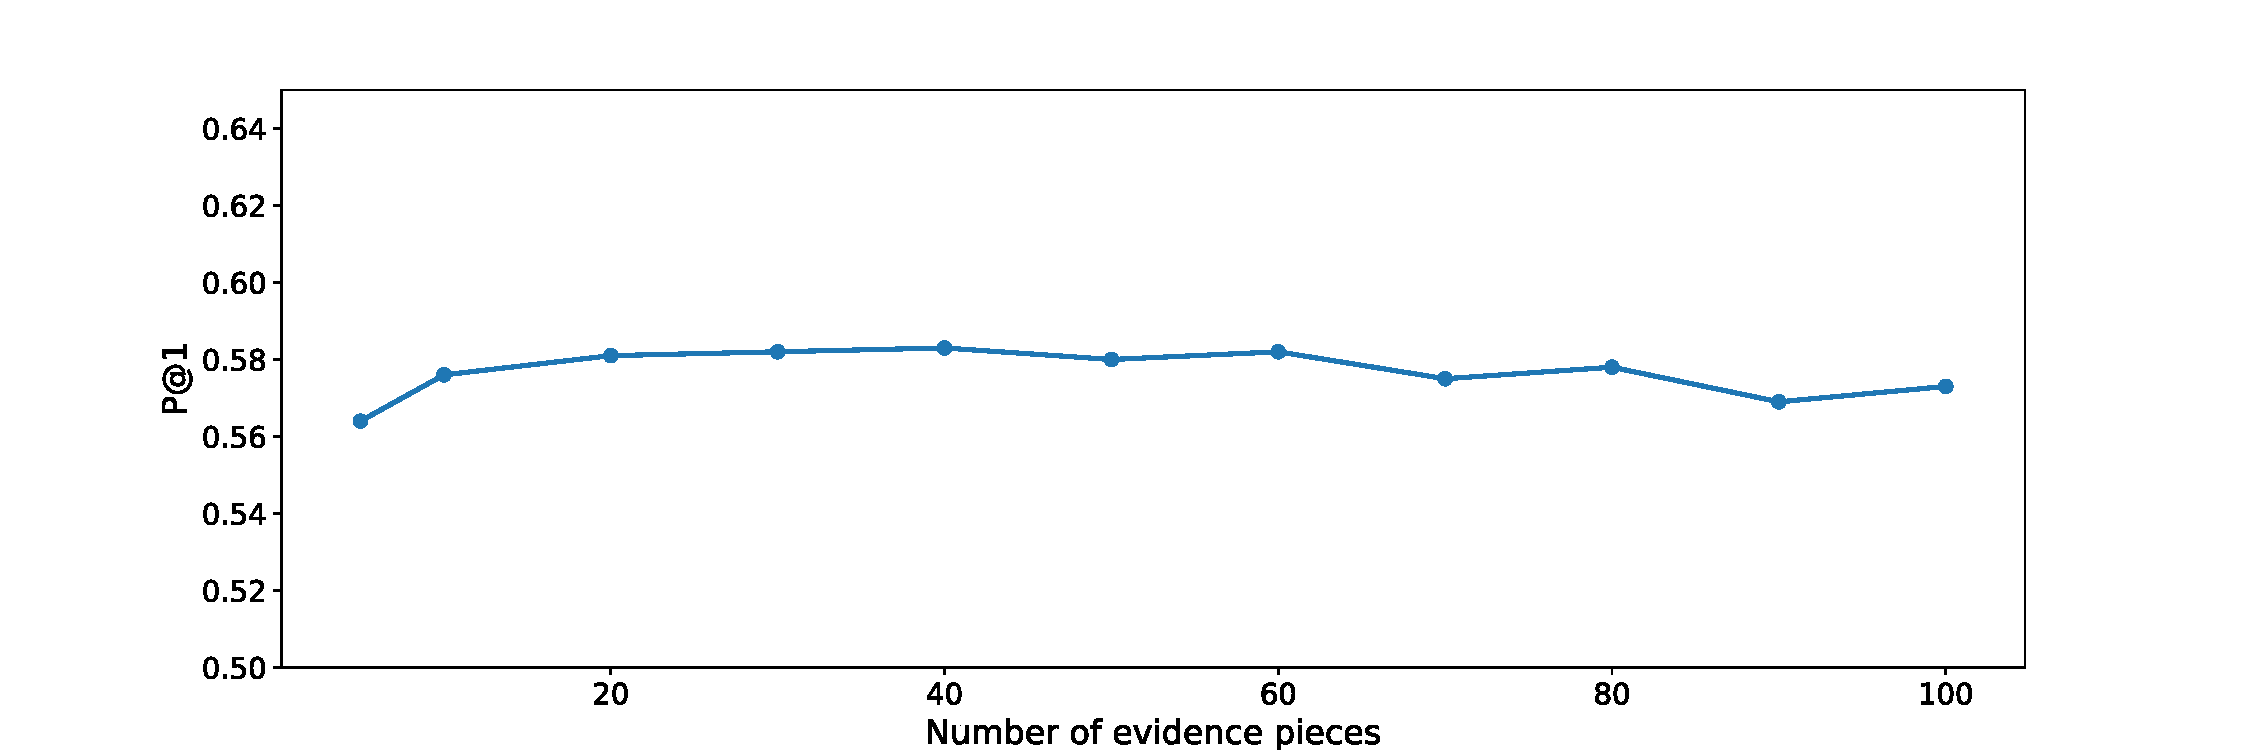
\includegraphics[width=0.8\textwidth]{submissions/Gerhard2024/figures/p_at_1-line_with_evidences.pdf}
    \vspace*{-0.2cm}
    \caption{Performance of \method on the \compmix dev set with different numbers of evidence.}
    \label{fig:res-num-evidences}
    \vspace*{-0.2cm}
\end{figure}



%%% ABLATION
\myparagraph{Ablation study on re-ranking} For more insight on the possible configurations of the RF stage, we conducted an ablation study with different options, including solely relying on the initial BM25 scoring without explicit re-ranking. The results are shown in Table \ref{tab:ablation2}. We observe that the iterative reduction in two steps is slightly better than the single-step variants (going down from top-1000 to top-30 in one RF step). Between the two options of using a GNN or a CE, the differences are negligible. A notable effect is that our RF techniques retain the answer presence at a very high level, only a bit lower than for the initial top-1000. 
The last two rows of Table \ref{tab:ablation2} demonstrate that RF is crucial: without explicit re-ranking, the technique of just picking smaller top-$k$ from the original BM25 model leads to substantial degradation in both answer presence and precision. 


\begin{table} [t] \small
    \centering
    \newcolumntype{G}{>{\columncolor [gray] {0.90}}c}
    \newcolumntype{H}{>{\setbox0=\hbox\bgroup}c<{\egroup}@{}}
    	\begin{tabular}{l G H G G G} 
        \toprule
            & \multicolumn{5}{G}{\textbf{\compmix} (dev set)} \\
        \midrule
            \textbf{RF Method $\downarrow$ / Metric $\rightarrow$} & \textbf{P@1} & \textbf{AP@1000} & \textbf{AP@100}  & \textbf{AP@30} & \textbf{MRR@100} \\ 
        \midrule
            \textbf{GNN: 1000 $\rightarrow$ 100 $\rightarrow$ 30}             &  $\mathbf{0.574}$  & $0.760$ &  $0.738$  &  $0.710$  &  $\mathbf{0.572}$  \\
            \textbf{CE: 1000 $\rightarrow$ 100 $\rightarrow$ 30}          &  $0.573$  & $0.760$  &   $\mathbf{0.740}$ &  $\mathbf{0.721}$   &  $0.553$   \\
        \midrule
            \textbf{GNN: 1000 $\rightarrow$ 30} &  $0.567$  & $?$  &   $n/a$ &  $0.710$   &  $0.567$   \\
         \textbf{CE: 1000 $\rightarrow$ 30} &  $0.570$  & $0.760$  &   $n/a$ &  $0.715$   &  $0.558$   \\
            \midrule
           \textbf{BM25: 100 (w/o GNN or CE)} &  $0.490$ & $0.760$  &  $0.652$  &  $n/a$  &  $0.259$ \\       
            \textbf{BM25: 30 (w/o GNN or CE)} &  $0.468$  & $0.760$  &  $n/a$ &  $0.534$   &  $0.259$   \\
            \bottomrule
    \end{tabular}
    \vspace*{-0.2cm}
    \caption{Ablation study for different RF strategies of \method on the \compmix dev set. The answer presence in the RF input with top-$1000$ evidence pieces is $0.760$.}
    \label{tab:ablation2}
\end{table}



\myparagraph{Quality of SI}
To assess the quality and robustness of the Structured Intents, we
inspected a sample of questions and their SIs.
Table~\ref{tab:question-SI-examples} gives three anecdotic examples.
We show SIs generated by \method, which makes use of the pre-existing collection from the \compmix benchmark for training.
This training data was obtained via different heuristics, 
which can be a limiting factor when user intents become more complex.

Therefore, we also looked at SIs derived via in-context learning (ICL) using \gptfour with $5$ handcrafted examples.
As shown in our earlier work on temporal QA~\cite{Jia-FAITH:WWW2024},
such data can be used for training smaller models (e.g., BART),
which can greatly boost the completeness and overall quality of the generated SIs.

From the sampled set, we observed that the ICL-based SIs are more
complete with all slots filled, whereas the BART-based SIs focused more
on the main slots Answer-type, Entities and Relation.
However, both approaches achieve very high quality in filling the slots,
capturing the user's information need very well.

Interestingly, when questions get complicated, with nested phrases, 
the ICL-based variant succeeds in decomposing the questions, based on only $5$ ICL examples.
For example, for the question {\em ``which German state had the most Corona-related death cases in the first year after the outbreak?''}
the Time slot becomes {\em ``first year after Corona outbreak''},
which can be resolved to identify the temporal scope.
In general, we believe that such question decomposition, beyond simple temporal constraints,
would be an interesting theme for future work.

\begin{table} [t] 
    \centering
    \small
    \newcolumntype{G}{>{\columncolor [gray] {0.90}}c}
    \newcolumntype{H}{>{\setbox0=\hbox\bgroup}c<{\egroup}@{}}
    \resizebox*{\textwidth}{!}{
        \begin{tabular}{p{6cm}|p{6cm}|p{6cm}} 
        \toprule
            \textbf{Question} & \textbf{Current SI by \method} & \textbf{SI via ICL} \\
        \midrule
        \textit{what was disneys first color movie?}
            & Ans-Type: \textit{animated feature film} & Ans-Type: \textit{film, animated film} \\
            & Entities: \textit{disneys} & Entities: \textit{Disney} \\
            & Relation: \textit{was first color movie} & Relation: \textit{first color movie} \\
            &  & Time: \textit{first} \\
        \midrule
        \textit{at the oscars, who won best actor in 2018?}
            & Ans-Type: \textit{human} & Ans-Type: \textit{person, actor} \\
            & Entities: \textit{at the oscars} & Entities: \textit{Oscars, 2018} \\
            & Relation: \textit{who won best actor in 2018} & Relation: \textit{won best actor} \\
            &  & Time: \textit{2018} \\
        \midrule
        \textit{which German state had the most Corona-} & Ans-Type: \textit{state} & Ans-Type: \textit{location, state} \\
        \textit{related death cases in the first year after} & Entities: \textit{Germany, Corona} & Entities: \textit{Germany, Corona-related deaths} \\
        \textit{the outbreak?} & Relation: \textit{which state had the most related} & Relation: \textit{highest count of death cases} \\
        & \textit{death cases in the first year after the out-}  & Location: \textit{Germany} \\
            & \textit{break}  & Time: \textit{first year after Corona outbreak} \\
        \bottomrule
    \end{tabular}
    }
    \vspace*{-0.2cm}
    \caption{Examples for pairs of question and generated SI.}
    \label{tab:question-SI-examples}
\end{table}




%%% REFRAIN FROM ANSWER
\myparagraph{Refraining from answering}
%%% Searched for: "generated_answer I" (with I being the full word, not partial) in the generated answers of LLaMA
%%% yields 245 results out of 2764 questions on CompMix
%%% yields 1270 results out of 3237 questions on TimeQuestions
We can train our model to refrain from answering in scenarios
where the provided evidence does not contain an answer to the question.
Specifically, during training, when the answer is not present in the evidence,
we change the target answer to {\em unknown}. This variant is referred to as \method {\em (faithful)}.

We measure the ratio of questions for which {\em unknown} is provided as answer,
and the P@1 restricted to questions that are answered.
The accuracy of refraining from answering is measured as well,
based on whether the answer is present in the evidence or not.
We conduct this experiment on \compmix and \timequestions,
for which we can compute answer presence exactly.
We also compute results for \llama, which is already instructed 
with the option to answer ``don't know''.
Table~\ref{tab:refrain-from-answer} shows the results.
For \compmix, we observe that \method has high accuracy on refraining when appropriate,
whereas \llama tends to be overconfident with a very small rate of {\em unknowns}, leading to incorrect answers.

\begin{table} [t] \small
    \centering
    \newcolumntype{G}{>{\columncolor [gray] {0.90}}c}
    \newcolumntype{H}{>{\setbox0=\hbox\bgroup}c<{\egroup}@{}}
    	\begin{tabular}{l G G G G c c c c} 
        \toprule
            & \multicolumn{4}{G}{\textbf{\compmix}} & \multicolumn{4}{c}{\textbf{\timequestions}} \\
            \midrule
            \textbf{Metric $\rightarrow$} & \textbf{P@1}  & \textbf{P@1} & \textbf{Refrain} & \textbf{Refrain} & \textbf{P@1}  & \textbf{P@1} & \textbf{Refrain} & \textbf{Refrain} \\ 
            \textbf{Method $\downarrow$} &                 & \textbf{(answered)} & \textbf{rate} & \textbf{accuracy} &                 & \textbf{(answered)} & \textbf{rate} & \textbf{accuracy} \\ 
            \midrule
                \textbf{\llama}             &  $0.431$  &  $0.471$  &  $0.089$  &  $n/a$  &  $0.177$  &  $0.276$  &  $0.392$  &  $n/a$  \\
                \textbf{\method (faithful)}           &  $0.497$  &  $0.713$  &  $0.303$  &  $0.838$ &  $0.597$  &  $0.804$  &  $0.257$  &  $0.864$  \\
            \bottomrule
    \end{tabular}
    \vspace*{-0.2cm}
    \caption{
        Performance of \method with option to refrain from answering (``don't know'').
    }
    \label{tab:refrain-from-answer}
\end{table}

\label{sec:disc}
\section{Insights, Limitations, and Challenges}


\noindent{\bf Benchmark Performance.} Our method, RAG-based \method with an 8B LLaMA model, outperforms much larger LLMs like \gptfour on two of the three benchmarks, with a very large margin for temporal questions. Obviously, pre-trained LLMs have only limited sense of properly positioning ``remembered’’ facts on the timeline even with training data that exceeds ours by several orders of magnitude. This confirms our intuition that LLMs alone are not good at ``recalling’’  higher-arity relations that require combining distant pieces of evidence. This is a sweet spot for RAG. Only for 
the \crag benchmark, \method is substantially inferior to a full-blown LLM. This is likely due to the nature of the questions: not necessarily the complexity of the information needs, but the need for more web sources (beyond what our experiments tap into).

\vspace{0.2cm}
\noindent{\bf Cost/Performance Ratio.} The most important take-away from our experiments is that \method achieves its competitive performance at a much lower cost than the full LLMs. Assuming that the consumed GFlops are proportional to the number of model parameters, \method achieves a cost reduction by a factor of 200x for \gptthree and 2000x for \gptfour. This does not only mean less computation, but also a massively lower electricity bill and climate impact.  

\vspace{0.2cm}
\noindent{\bf Role of Question Understanding.} We did not systematically investigate the influence of the Structured Intent in the \method pipeline. However, the comparison to the big GPT models reflects the role of the SI, as we prompt the GPT models in their natural mode with the original questions. The linearized sequence of available SI slots does not always have major advantages, but there are enough cases where specific facets provide crucial cues. This holds especially for the Entities slot, as this drives the gathering of evidence in the ER stage (cf.~\cite{Christmann-CONVINSE:SIGIR2022}, and for the Time slot, as these cues are often decisive for temporal questions (cf.~\cite{Jia-FAITH:WWW2024}).

\vspace{0.2cm}
\noindent{\bf Role of Re-Ranking.} As our ablation studies show, merely using top-$k$ evidence from an initial BM25-style ranking does not provide good performance. Also, there seems to be sweet spot in the choice of $k$: we need enough evidence for connecting the dots if the question requires multiple pieces of information, or for corroborating candidates if the question finds many useful but noisy pieces. In the experiments, $k=30$ turns out to be good choice; much lower $k$ results in insufficient evidence, and much larger $k$ leads to saturation and ultimately degrading performance. Our argument for iteratively shrinking the candidate set in multiple rounds of re-ranking is substantiated in our experiments, but the gain of doing this, compared to GNN- or CE-based re-ranking from 1000 to 30, is not big. More research is called to better understand the role of ranking in RAG. 

\vspace{0.2cm}
\noindent{\bf Limitations of Evidence Retrieval.}
For ER, we adopted more or less standard techniques. The results showed very good answer presence, in the order of 75\% in the top-100 or even top-30. An important case where this is insufficient are questions that require aggregating information over a large number of evidence pieces. An example is asking for the life-time total of 3-point scores of the basketball player Dirk Nowitzki.
This requires collecting a set of per-season tables with NBA player statistics, but also other web sources with numbers for his career before he joined the NBA (including his youth teams).
Of course, there are sometimes shortcuts like a Wikipedia article or biography mentioning the total number, but this cannot be universally assumed. The bottom line is that ER should be reconsidered as well, striving to improve the recall dimension.

\vspace{0.2cm}
\noindent{\bf Limitations of Answer Generation.}
For AG, we simply rely on a LLM,
using it as an extractor (``reader'') from the given evidence. Despite the wide belief that LLMs can perform deep
reasoning over many pieces of evidence, our experience is that the extraction works only well – robustly and faithfully – for relatively simple questions with a few multi-hop joins or simple aggregation over a few pieces. However, complicated questions such as asking for the top-100 NBA players with the largest number of life-time 3-point scores (again including their pre-NBA careers) are currently out of scope and will likely remain so for quite some time. This offers many opportunities for pushing the envelope further.

\vspace{0.2cm}
\noindent{\bf Trust in Data Sources.}
In our experiments, we considered all heterogeneous sources as trustworthy and unbiased. With focus on Wikidata and Wikipedia, this assumption has been well justified. In the wild, however, input data for RAG-based systems likely exhibit a wide spectrum of quality issues, in terms of stale information, biased positions, or simply false statements. Identifying trustworthy and up-to-date evidence and dealing with conflicting data, has been explored in other contexts (e.g., for KG curation~\cite{Dong-Trust:PVLDB2015}), but remains a major challenge for RAG-based QA.


\vspace{0.2cm}
\noindent{\bf Open Challenges and Future Work.} The best-performing methods in our experiment, mostly \method, reach P@1 values of 56\% for \compmix and 75\% for \timequestions. 
For the latter, the answer presence in the top-100 is only slightly higher; so the AG stage hardly misses anything.
However, for \compmix, the answer presence is 75\% -- much higher than what our system can actually answer. Obviously, closing this gap is a major direction to pursue, with focus on the RF and AG stages. However, missing one fourth of the answers completely in the top-100 pool, is a big problem as well. This requires improving recall at the ER stage, possibly with better guidance by the QU, which in turn needs more sources beyond the scope of our experiments (currently limited to Wikidata and Wikipedia). 

In general, we need to think beyond this kind of ``benchmark mindset’’. Even if we reached 80\% or 90\% precision and recall, we would still have a substantial fraction of questions that are answered incorrectly
or not at all. 
The remaining errors may not be a problem for chatbots, but they would be a showstopper for the deployment of mission-critical applications in business or science. We believe that this big gap is a shortcoming of {\em all methods}, not an issue that comes from the data alone. For trivia-style QA, as looked at in this paper, a smart human in ``open book’’ mode and no time limitation should be able to properly answer practically all questions, just by reading pieces of web contents and putting things together. Neither LLMs nor state-of-the-art RAG are the final solution; substantial research and creative ideas are needed to further advance QA.


\clearpage
\newpage

\newcommand{\bibauthors}[1]{{#1}}
\newcommand{\bibtitle}[1]{\emph{#1}}
\newcommand{\bibconf}[1]{{#1}}

\begin{thebibliography}{10}

\bibitem{Bajaj:arxiv2018}
\bibauthors{Payal Bajaj, Daniel Campos, Nick Craswell, Li Deng, Jianfeng Gao, Xiaodong Liu, Rangan Majumder, Andrew McNamara, Bhaskar Mitra, Tri Nguyen, Mir Rosenberg, Xia Song, Alina Stoica, Saurabh Tiwary, Tong Wang.}
\bibtitle{MS MARCO: A Human Generated MAchine Reading COmprehension Dataset.}
In \bibconf{arXiv 2018}.

\bibitem{DBLP:conf/acl/ChenFWB17}
\bibauthors{Danqi Chen, Adam Fisch, Jason Weston and Antoine Bordes.}
\bibtitle{Reading Wikipedia to Answer Open-Domain Questions.}
In \bibconf{ACL 2017}.

\bibitem{Christmann-CONVINSE:SIGIR2022}
\bibauthors{Philipp Christmann, Rishiraj Saha Roy, Gerhard Weikum.}
\bibtitle{Conversational Question Answering on Heterogeneous Sources.}
In \bibconf{SIGIR 2022}.

\bibitem{Christmann-CLOCQ:WSDM2022}
\bibauthors{Philipp Christmann, Rishiraj Saha Roy, Gerhard Weikum.}
\bibtitle{Beyond NED: Fast and Effective Search Space Reduction for Complex Question Answering over Knowledge Bases.}
In \bibconf{WSDM 2022}.

\bibitem{Christmann-Explaignn:SIGIR2023}
\bibauthors{Philipp Christmann, Rishiraj Saha Roy, Gerhard Weikum.}
\bibtitle{Explainable Conversational Question Answering over Heterogeneous Sources via Iterative Graph Neural Networks.}
In \bibconf{SIGIR 2023}.

\bibitem{Christmann-CompMix:WWW2024}
\bibauthors{Philipp Christmann, Rishiraj Saha Roy, Gerhard Weikum.}
\bibtitle{CompMix: A Benchmark for Heterogeneous Question Answering.}
In \bibconf{WWW 2024}.

\bibitem{Dejean:arxiv2024}
\bibauthors{Herve Dejean, Stephane Clinchant, Thibault Formal.}
\bibtitle{A Thorough Comparison of Cross-Encoders and LLMs for Reranking SPLADE.}
In \bibconf{arXiv 2024}.

\bibitem{Dhingra-time-aware-LLM:TACL2022}
\bibauthors{Bhuwan Dhingra, Jeremy R Cole, Julian Martin Eisenschlos, Daniel Gillick, Jacob Eisenstein, and William W Cohen.}
\bibtitle{Time-Aware Language Models as Temporal Knowledge Bases.}
In \bibconf{TACL 2022}.

\bibitem{Dong-Trust:PVLDB2015}
\bibauthors{Xin Luna Dong, Evgeniy Gabrilovich, Kevin Murphy, Van Dang, Wilko Horn, Camillo Lugaresi, Shaohua Sun, Wei Zhang.}
\bibtitle{Knowledge-Based Trust: Estimating the Trustworthiness of Web Sources.}
In \bibconf{PVLDB 2015}.

\bibitem{DBLP:journals/arXiv/abs-2312-10997}
\bibauthors{Yunfan Gao, Yun Xiong, Xinyu Gao, Kangxiang Jia, Jinliu Pan, Yuxi Bi, Yi Dai, Jiawei Sun, Qianyu Guo, Meng Wang, Haofen Wang.}
\bibtitle{Retrieval-Augmented Generation for Large Language Models: A Survey.}
In \bibconf{arXiv 2023}.

\bibitem{Gao-citations:emnlp2023}
\bibauthors{Tianyu Gao, Howard Yen, Jiatong Yu, Danqi Chen.}
\bibtitle{Enabling Large Language Models to Generate Text with Citations.}
In \bibconf{EMNLP 2023}.

\bibitem{Guu-REALM:ICML2020}
\bibauthors{Kelvin Guu, Kenton Lee, Zora Tung, Panupong Pasupat, Ming-Wei Chang.}
\bibtitle{Retrieval Augmented Language Model Pre-Training.}
In \bibconf{ICML 2020}.

\bibitem{DBLP:conf/eacl/IzacardG21}
\bibauthors{Gautier Izacard, Edouard Grave.}
\bibtitle{Leveraging Passage Retrieval with Generative Models for Open Domain Question Answering.}
In \bibconf{EACL 2021}.

\bibitem{Jia-TimeQuestions}
\bibauthors{Zhen Jia, Soumajit Pramanik, Rishiraj Saha Roy, and Gerhard Weikum.}
\bibtitle{Complex Temporal Question Answering on Knowledge Graphs.}
In \bibconf{CIKM 2021}.

\bibitem{Jia-FAITH:WWW2024}
\bibauthors{Zhen Jia, Philipp Christmann, Gerhard Weikum.}
\bibtitle{Faithful Temporal Question Answering over Heterogeneous Sources.}
In \bibconf{WWW 2024}.

\bibitem{DBLP:journals/arXiv/abs-2305-06984}
\bibauthors{Ehsan Kamalloo, Nouha Dziri, Charles L. A. Clarke, Davood Rafiei.}
\bibtitle{Evaluating Open-Domain Question Answering in the Era of Large Language Models.}
In \bibconf{arXiv 2023}.

\bibitem{Kandpal:ICML2023}
\bibauthors{Nikhil Kandpal, Haikang Deng, Adam Roberts, Eric Wallace, Colin Raffel.}
\bibtitle{Large Language Models Struggle to Learn Long-Tail Knowledge.}
In \bibconf{ICML 2023}.

\bibitem{DBLP:conf/emnlp/KarpukhinOMLWEC20}
\bibauthors{Vladimir Karpukhin, Barlas Oguz, Sewon Min, Patrick S. H. Lewis, Ledell Wu, Sergey Edunov, Danqi Chen, Wen-tau Yih.}
\bibtitle{Dense Passage Retrieval for Open-Domain Question Answering.}
In \bibconf{EMNLP 2020}.

\bibitem{Lee-MATTER:ACL2024}
\bibauthors{Dongkyu Lee, Chandana Satya Prakash, Jack FitzGerald, Jens Lehmann.}
\bibtitle{MATTER: Memory-Augmented Transformer Using Heterogeneous Knowledge Sources.}
In \bibconf{ACL 2024}.

\bibitem{DBLP:conf/acl/LewisLGGMLSZ20}
\bibauthors{Mike Lewis, Yinhan Liu, Naman Goyal, Marjan Ghazvininejad, Abdelrahman Mohamed, Omer Levy, Veselin Stoyanov, Luke Zettlemoyer.}
\bibtitle{BART: Denoising Sequence-to-Sequence Pre-training for Natural Language Generation, Translation, and Comprehension.}
In \bibconf{ACL 2020}.

\bibitem{DBLP:conf/nips/LewisPPPKGKLYR020}
\bibauthors{Patrick S. H. Lewis, Ethan Perez, Aleksandra Piktus, Fabio Petroni, Vladimir Karpukhin, Naman Goyal, Heinrich Küttler, Mike Lewis, Wen-tau Yih, Tim Rocktäschel, Sebastian Riedel, Douwe Kiela.}
\bibtitle{Retrieval-Augmented Generation for Knowledge-Intensive NLP Tasks.}
In \bibconf{NeurIPS 2020}.

\bibitem{Lin:MC2021}
\bibauthors{Jimmy Lin, Rodrigo Frassetto Nogueira, Andrew Yates.}
\bibtitle{Pretrained Transformers for Text Ranking: BERT and Beyond.}
In \bibconf{Morgan \& Claypool Publishers 2021}.

\bibitem{Liu-SUQL:NAACL2024}
\bibauthors{Shicheng Liu, Jialiang Xu, Wesley Tjangnaka, Sina J. Semnani, Chen Jie Yu, Monica Lam.}
\bibtitle{SUQL: Conversational Search over Structured and Unstructured Data with Large Language Models.}
In \bibconf{NAACL-HLT 2024}.

\bibitem{Mavi:FnT2024}
\bibauthors{Vaibhav Mavi, Anubhav Jangra, Adam Jatowt.}
\bibtitle{Multi-hop Question Answering.}
In \bibconf{Foundations and Trends in Information Retrieval 2024}.

\bibitem{Minaee-LLM-survey}
\bibauthors{Shervin Minaee, Tomas Mikolov, Narjes Nikzad, Meysam Chenaghlu, Richard}
\bibtitle{Socher, Xavier Amatriain, and Jianfeng Gao.}
Large Language Models: A Survey.
In \bibconf{arXiv 2024}.

\bibitem{Nogueira:arxiv2019}
\bibauthors{Rodrigo Frassetto Nogueira, Kyunghyun Cho.}
\bibtitle{Passage Re-ranking with BERT.}
In \bibconf{arXiv 2019}.

\bibitem{Oguz-UniK-QA:NAACL2022}
\bibauthors{Barlas Oguz, Xilun Chen, Vladimir Karpukhin, Stan Peshterliev, Dmytro Okhonko, Michael Sejr Schlichtkrull, Sonal Gupta, Yashar Mehdad, Scott Yih.}
\bibtitle{UniK-QA: Unified Representations of Structured and Unstructured Knowledge for Open-Domain Question Answering.}
In \bibconf{NAACL-HLT 2022}.

\bibitem{RogersGA:CS2023}
\bibauthors{Anna Rogers, Matt Gardner, Isabelle Augenstein.}
\bibtitle{QA Dataset Explosion: A Taxonomy of NLP Resources for Question Answering and Reading Comprehension.}
In \bibconf{ACM Computing Surveys 2023}.

\bibitem{RoyAnand:MC2021}
\bibauthors{Rishiraj Saha Roy, Avishek Anand.}
\bibtitle{Question Answering for the Curated Web: Tasks and Methods in QA over Knowledge Bases and Text Collections.}
In \bibconf{Synthesis Lectures on Information Concepts, Retrieval, and Services, Morgan \& Claypool Publishers 2021}.

\bibitem{Pramanik-Uniqorn:JWS2024}
\bibauthors{Soumajit Pramanik, Jesujoba Alabi, Rishiraj Saha Roy, Gerhard Weikum.}
\bibtitle{UNIQORN: Unified Question Answering over RDF Knowledge Graphs and Natural Language Text.}
In \bibconf{Journal of Web Semantics 2024}.

\bibitem{Sun-PullNet:EMNLP2019}
\bibauthors{Haitian Sun, Tania Bedrax-Weiss, William W. Cohen.}
\bibtitle{PullNet: Open Domain Question Answering with Iterative Retrieval on Knowledge Bases and Text.}
In \bibconf{EMNLP/IJCNLP 2019}.

\bibitem{Sun:NAACL2024}
\bibauthors{Kai Sun, Yifan Ethan Xu, Hanwen Zha, Yue Liu, Xin Luna Dong.}
\bibtitle{Head-to-Tail: How Knowledgeable are Large Language Models (LLMs)? A.K.A. Will LLMs Replace Knowledge Graphs?}
In \bibconf{NAACL-HLT 2024}.

\bibitem{Touvron-LLaMA}
\bibauthors{Hugo Touvron, Thibaut Lavril, Gautier Izacard, Xavier Martinet, Marie-Anne Lachaux, Timothée Lacroix, Baptiste Rozière, Naman Goyal, Eric Hambro, Faisal Azhar, Aurelien Rodriguez, Armand Joulin, Edouard Grave, Guillaume Lample.}
\bibtitle{Llama: Open and efficient foundation language models.}
In \bibconf{arXiv 2023}.

\bibitem{Wu-STARK:arxiv2024}
\bibauthors{Shirley Wu, Shiyu Zhao, Michihiro Yasunaga, Kexin Huang, Kaidi Cao, Qian Huang, Vassilis N. Ioannidis, Karthik Subbian, James Zou, Jure Leskovec.}
\bibtitle{STaRK: Benchmarking LLM Retrieval on Textual and Relational Knowledge Bases.}
In \bibconf{arXiv 2024}.

\bibitem{Wu:IEEE2021}
\bibauthors{Zonghan Wu, Shirui Pan, Fengwen Chen, Guodong Long, Chengqi Zhang, Philip S. Yu.}
\bibtitle{A Comprehensive Survey on Graph Neural Networks.}
In \bibconf{IEEE Transactions on Neural Networks and Learning Systems 2021}.

\bibitem{Yang-CRAG}
\bibauthors{Xiao Yang, Kai Sun, Hao Xin, Yushi Sun, Nikita Bhalla, Xiangsen Chen, Sajal Choudhary, Rongze D. Gui, Ziran W. Jiang, Ziyu Jiang, Lingkun Kong, Brian Moran, Jiaqi Wang, Yifan Ethan Xu, An Yan, Chenyu Yang, Eting Yuan, Hanwen Zha, Nan Tang, Lei Chen, Nicolas Scheffer, Yue Liu, Nirav Shah, Rakesh Wanga, Anuj Kumar, Wen-tau Yih, Xin Luna Dong.}
\bibtitle{CRAG -- Comprehensive RAG Benchmark.}
In \bibconf{arXiv 2024}.

\bibitem{Yasunaga:NAACL2021}
\bibauthors{Michihiro Yasunaga, Hongyu Ren, Antoine Bosselut, Percy Liang, Jure Leskovec.}
\bibtitle{QA-GNN: Reasoning with Language Models and Knowledge Graphs for Question Answering.}
In \bibconf{NAACL-HLT 2021}.

\bibitem{Zhang-Spaghetti:ACL2024}
\bibauthors{Heidi C. Zhang, Sina J. Semnani, Farhad Ghassemi, Jialiang Xu, Shicheng Liu, Monica S. Lam.}
\bibtitle{SPAGHETTI: Open-Domain Question Answering from Heterogeneous Data Sources with Retrieval and Semantic Parsing.}
In \bibconf{ACL 2024}.

\bibitem{Zhang:NAACL2024}
\bibauthors{Jiahao Zhang, Haiyang Zhang, Dongmei Zhang, Yong Liu, Shen Huang.}
\bibtitle{End-to-End Beam Retrieval for Multi-Hop Question Answering.}
In \bibconf{NAACL-HLT 2024}.

\bibitem{Zhao-LLMsurvey}
\bibauthors{Wayne Xin Zhao, Kun Zhou, Junyi Li, Tianyi Tang, Xiaolei Wang, Yupeng Hou, Yingqian Min, Beichen Zhang, Junjie Zhang, Zican Dong, Yifan Du, Chen Yang, Yushuo Chen, Zhipeng Chen, Jinhao Jiang, Ruiyang Ren, Yifan Li, Xinyu Tang, Zikang Liu, Peiyu Liu, Jian-Yun Nie, Ji-Rong Wen.}
\bibtitle{A Survey of Large Language Models.}
In \bibconf{arXiv 2023}.

\bibitem{Zhao:arxiv2024}
\bibauthors{Penghao Zhao, Hailin Zhang, Qinhan Yu, Zhengren Wang, Yunteng Geng, Fangcheng Fu, Ling Yang, Wentao Zhang, Bin Cui.}
\bibtitle{Retrieval-Augmented Generation for AI-Generated Content: A Survey.}
In \bibconf{arXiv 2024}.

\bibitem{Zhu-ODQA-survey:arxiv2021}
\bibauthors{Fengbin Zhu, Wenqiang Lei, Chao Wang, Jianming Zheng, Soujanya Poria, Tat-Seng Chua.}
\bibtitle{Retrieving and Reading: A Comprehensive Survey on Open-domain Question Answering.}
In \bibconf{arXiv 2021}.

\end{thebibliography}


\end{document}

\end{article}
\begin{article}
{Episodic Memory Integration of Personal Data in YourDigitalSelf}
{Varvara Kalokyri, Alexander Borgida, Amelie Marian}
\setcounter{section}{0}
\documentclass{article}

\usepackage{deauthor}

\usepackage{latexsym}
\usepackage{graphicx}
\graphicspath{{./images/}}
\usepackage{booktabs} % for formal tables
\usepackage{color}  % for coloring text
\usepackage{amsmath}  % for aligning equations
\usepackage{subcaption}
\usepackage{caption}
\usepackage{tikz}
\usepackage{colortbl} % for color in tables
\usepackage{framed}
\usepackage{multirow}
\usepackage{multicol}
\usepackage{hyperref}
\usepackage{url}
\usepackage{balance}
\usepackage{verbatim}
\usepackage{cancel}
\usepackage{xspace} % for correcting space after macro commands
\usepackage{algorithm2e}
\usepackage{bbold} % for writing mathbb{1}
\usepackage{balance}
\usepackage{stmaryrd}
\usepackage{enumitem}
\usepackage{array} % package for hiding a column
\usepackage{bold-extra} % to enable textbf with textsc

% used for making text readable in document and .tex
% \setlength{\parindent}{0pt}

\newcommand{\struct}[1]{\texttt{\small #1}}
\newcommand{\utterance}[1]{\textit{#1}}
\newcommand{\phrase}[1]{\textit{``#1''}}

% \newcommand {\g}[1]{\textcolor[gray]{0.6}{#1}}

\newcommand{\drop}{\dag\xspace}

\newenvironment{Snugshade}[1][236,236,236]{
    \setlength{\itemsep}{0pt}
     \setlength{\parsep}{0pt}
     \setlength{\topsep}{0pt}
     \setlength{\partopsep}{0pt}
     \setlength{\leftmargin}{1.5em}
     \setlength{\labelwidth}{0em}
     \setlength{\labelsep}{0em} 
    \setlength{\parskip}{0pt}
    \definecolor{shadecolor}{RGB}{#1}
    \begin{snugshade}
}{
    \end{snugshade}
}


\newcommand{\method}{\textsc{Quasar}\xspace}
\newcommand{\benchmark}{\textsc{PerQA}\xspace}
\newcommand{\itemslist}[1]{$\langle$\struct{#1}$\rangle$}


\newcommand{\convinse}{\textsc{Convinse}\xspace}
\newcommand{\explaignn}{\textsc{Explaignn}\xspace}
\newcommand{\clocq}{\textsc{Clocq}\xspace}
\newcommand{\unikqa}{\textsc{UniK-Qa}\xspace}
\newcommand{\gptthree}{\textsc{Gpt-3}\xspace}
\newcommand{\gptfour}{\textsc{Gpt-4}\xspace}
\newcommand{\llama}{\textsc{Llama3}\xspace}
\newcommand{\spaghetti}{\textsc{Spaghetti}\xspace}


\newcommand{\compmix}{\textsc{CompMix}\xspace}
\newcommand{\timequestions}{\textsc{TimeQuestions}\xspace}
\newcommand{\crag}{\textsc{Crag}\xspace}


\newcommand{\squishlist}{
    \begin{list}{$\bullet$}{
        \setlength{\itemsep}{0pt}
	\setlength{\parsep}{3pt}
	\setlength{\topsep}{3pt}
	\setlength{\partopsep}{0pt}
	\setlength{\leftmargin}{1.5em}
	\setlength{\labelwidth}{1em}
	\setlength{\labelsep}{0.5em}
    }
}

\newcommand{\squishend}{
    \end{list}
}

\newcommand{\myparagraph}[1]{\vspace*{0.2cm}\noindent \textbf{#1}.}
\newcommand{\myparagraphnospace}[1]{\noindent \textbf{#1}.}

% \newcommand{\GW}[1]{\emph{{\color{blue} GW:#1}}}
% \newcommand{\PC}[1]{\emph{{\color{orange} PC: #1}}}
% \newcommand{\tocite}{{{\color{red} [CITE]}}}


\begin{document}

\title{RAG-based Question Answering \\ over Heterogeneous Data and Text}

\author{
Philipp Christmann,
Gerhard Weikum\\\\
Max Planck Institute for Informatics\\
Saarland Informatics Campus, Germany\\
\texttt{\{pchristm, weikum\}@mpi-inf.mpg.de}}

\maketitle

\section*{Abstract}
This article presents the \method system for question answering over unstructured text, structured tables, and knowledge graphs, with unified treatment of all sources.
The system adopts a RAG-based architecture, with a pipeline of evidence retrieval followed by answer generation, with the latter powered by a 
moderate-sized
language model.
Additionally and uniquely, \method
has components for question understanding, to derive crisper input for evidence retrieval, and for re-ranking and filtering the retrieved evidence before feeding the most informative pieces into the answer generation.
Experiments with three different benchmarks demonstrate the high answering quality of our approach, being on par with or better than large GPT models, while keeping the computational cost and energy consumption orders of magnitude lower.

\label{sec:intro}
\section{Introduction}

\noindent\textbf{Motivation and Problem.} The task of question answering, QA for short, arises in many flavors: factual vs. opinions, simple lookups vs. multi-hop inference, single answer vs. list of entities, 
direct answers vs. long-form, one-shot questions vs. conversations, and other varieties 
(see, e.g., surveys~\cite{RogersGA:CS2023,RoyAnand:MC2021}).
The state-of-the-art for this entire spectrum has been greatly advanced in the past decade. Most notably, incorporating deep learning into retriever-reader architectures (e.g.,~\cite{DBLP:conf/acl/ChenFWB17,DBLP:conf/eacl/IzacardG21,DBLP:conf/emnlp/KarpukhinOMLWEC20}) has boosted answering quality, and most recently, large language models (LLM)~\cite{Minaee-LLM-survey,Zhao-LLMsurvey} have pushed the envelope even further (e.g.,~\cite{DBLP:journals/arXiv/abs-2305-06984}).

% strengths and limitations of LLM for QA
Today’s LLMs alone are capable of accurately answering many \textit{factoid} questions, simply from their pre-trained parametric memory which latently encodes huge text corpora and other online contents.
However, this critically depends on the frequency of evidence in the underlying contents and the complexity of the information need. 
For example, 
asking for the {\em MVP of the 2024 NBA season} would easily return the correct answer Nikola Jokic, 
but asking for the {\em highest-scoring German NBA player} or the {\em MVP of the 2024 German basketball league} pose a big challenge.
The reason is that LLMs alone do not easily recall information about not so popular or even long-tail entities~\cite{Kandpal:ICML2023,Sun:NAACL2024},
and that they are mainly geared for direct look-ups as opposed to connecting multiple pieces of evidence~\cite{Mavi:FnT2024,Zhang:NAACL2024}.

% introduce RAG and discuss need for heterogeneous sources
\cite{DBLP:journals/arXiv/abs-2312-10997,Guu-REALM:ICML2020,DBLP:conf/nips/LewisPPPKGKLYR020,Zhao:arxiv2024}
known as RAG, address these bottlenecks. In addition to cleverly crafted prompts and few-shot examples, the LLM is provided with the top-ranked results of an explicit retrieval step, like web search or knowledge graph (KG) lookups. The former is often necessary for freshness of answers, and the latter may help with long-tail entities and also mitigate the notorious risk of hallucinations. Still, this generation’s RAG architectures are limited in how broad and how deep they tap into external sources. Popular AI assistants like Gemini or ChatGPT seem to primarily retrieve from the text of web pages (incl. Wikipedia articles), and academic research has additionally pursued knowledge augmentation by enhancing prompts with facts from large KGs (e.g., Wikidata).

An additional content modality that is still underexplored are {\em online tables}: a wide range of tabular data including HTML tables in web pages, spreadsheets and statistics, all the way to CSV and JSON datasets that are abundant on the Internet. There is prior work on joint support for text and KGs and for text and tables, but very little on all of these together -- some notable exceptions being~\cite{Christmann-CONVINSE:SIGIR2022,Christmann-Explaignn:SIGIR2023,Oguz-UniK-QA:NAACL2022,Zhang-Spaghetti:ACL2024}.


\noindent\textbf{Examples.} All three heterogeneous types of sources are crucial not only for answering different questions from different kinds of evidence, but also for combining multiple pieces of evidence of different modalities to infer correct and complete answers.
To 
illustrate
the need for tapping all sources, consider the following questions:

% \vspace*{0.2cm}
\begin{quote}
$Q1$: \utterance{Which Chinese basketballers have played in the NBA?}\\
 \indent $Q2$: \utterance{Who was the first Chinese NBA player?}\\
  \indent $Q3$: \utterance{Which Chinese NBA player has the most matches?}
\end{quote}
% \vspace*{0.2cm}

Q1 can be cast into querying a KG, but the list there is not necessarily complete and up-to-date, so additional evidence from text or tables would be desired. 
Q2 needs information about who played in which seasons, found only in web pages or sports-statistics tables. 
Finally, Q3 may be lucky in finding prominent textual evidence (e.g., in biographies, Wikipedia etc.), but this often faces divergent statements, and resolving contradictions needs to dive into more evidence. Besides, when textual evidence is rare and hard to find or not trustworthy enough, then information from multiple tables and text snippets may have to be aggregated (e.g., totals of per-season counts).
Some of this may perhaps become feasible for an industrial LLM’s RAG capabilities in the near future, but there are always harder scenarios by moving from Chinese NBA players deeper into the long tail, such as asking for {\em Lithuanian players in the German handball league}.

\vspace*{0.2cm}
\noindent\textbf{Approach and Contribution.} This paper presents a simple but powerful and versatile RAG system with unified access to text, KG and tables. We call our method {\em \method} 
(for Question Answering over Heterogeneous Sources with Augmented Retrieval).
Its architecture is relatively straightforward: all heterogeneous content is verbalized and indexed for retrieval; a retriever finds top-ranked results for the given question (from different source types), and these are fed into the LLM for answer generation. This is the unsurprising bird-eye’s view. Specific details that are key factors for the strong performance of \method are: 

\squishlist
\item[i)] automatically casting user questions into a structured representation of the information need, which is then used to guide 
\item[ii)] judicious ranking of search results, with multiple rounds of re-ranking and pruning, followed by
\item[iii)]	extracting faithful answers from an LLM in RAG mode, with answers grounded in tangible evidence.
\squishend


\vspace{0.2cm}
\noindent The paper presents experiments with three different benchmarks, covering various flavors of questions.
We focus on one-shot questions; conversational QA is out of scope here, but \method itself is well applicable to this case, too.
Our experiments demonstrate that our methods are competitive, on par with big GPT models and often better,
while being several orders of magnitude lower in computational and energy cost.
The experimental findings also highlight that question understanding, with structured representation of user intents, and iterative re-ranking of evidence are crucial for good performance.

Overall, our contribution lies in proposing a unified system architecture for RAG-based question answering over a suite of different data sources, with strong points regarding both effectiveness (i.e., answer quality)
and efficiency (i.e., computational cost).


\label{sec:background}
\section{Related Work}

The RAG paradigm came up as a principled way of enhancing LLM factuality incl. provenance and mitigating the risk of hallucination~\cite{Guu-REALM:ICML2020, DBLP:conf/nips/LewisPPPKGKLYR020}.
It is highly related to the earlier
retriever-reader architectures for QA~\cite{DBLP:conf/acl/ChenFWB17,DBLP:conf/emnlp/KarpukhinOMLWEC20}, especially when the reader uses the fusion-in-decoder method~\cite{DBLP:conf/eacl/IzacardG21,Oguz-UniK-QA:NAACL2022}.
Since its invention, RAG methodology has been greatly advanced, introducing a wide suite of extensions, such as batched inputs, interleaving retrieval and generation steps, and more (see the recent surveys~\cite{DBLP:journals/arXiv/abs-2312-10997,Zhao:arxiv2024}).

On question answering (QA), there is a vast amount of literature including a wealth of differently flavored benchmarks (see, e.g.,~\cite{RogersGA:CS2023}).
The case of interest here is QA over heterogeneous sources, tapping into both unstructured content and structured data. 
A variety of works has pursued this theme by combining knowledge graphs with text sources, using graph-based methods, neural learning and  language models (e.g.,~\cite{Pramanik-Uniqorn:JWS2024,Sun-PullNet:EMNLP2019,Yasunaga:NAACL2021}).

Most relevant for this article is the research on jointly leveraging all different sources: text, KGs, and tables (incl. CSV and JSON files). This includes  
the \unikqa system~\cite{Oguz-UniK-QA:NAACL2022},
the \spaghetti/SUQL project~\cite{Liu-SUQL:NAACL2024,Zhang-Spaghetti:ACL2024},
the \textsc{Matter} method~\cite{Lee-MATTER:ACL2024},
the STaRK benchmarking~\cite{Wu-STARK:arxiv2024},
and our own prior work
~\cite{Christmann-CONVINSE:SIGIR2022,Christmann-Explaignn:SIGIR2023} (without claiming exhaustiveness).
Out of these, we include \unikqa, \spaghetti and our own systems \convinse and \explaignn as baselines in the experimental evaluation.
Their architectures are similar to ours, but \unikqa and \spaghetti do not have our distinctive elements of
question understanding and iterative re-ranking (originally introduced in \explaignn~\cite{Christmann-Explaignn:SIGIR2023}).

\label{sec:method}
\section{Methodology}

\begin{figure}[tb]
  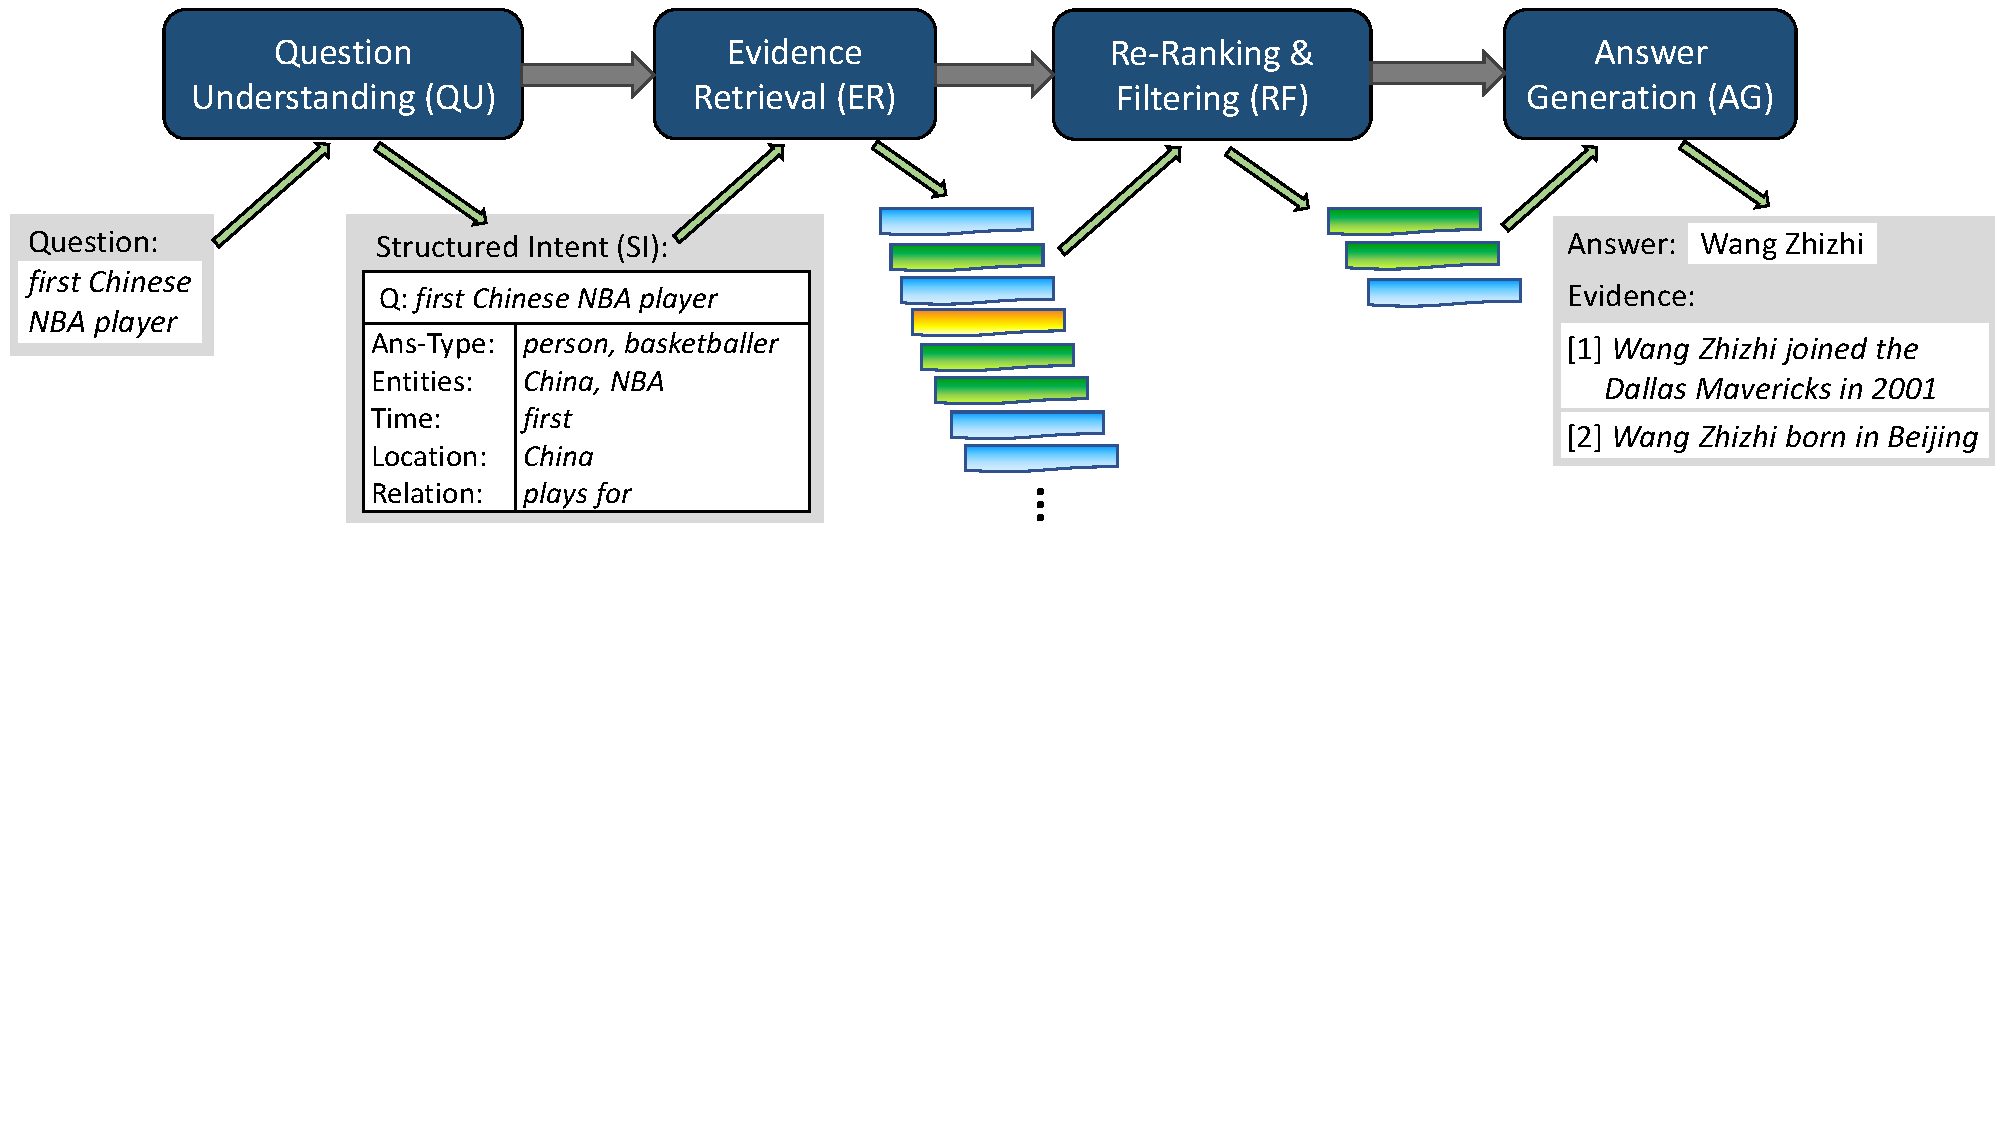
\includegraphics[width=\textwidth]{submissions/Gerhard2024/figures/compass-overview.pdf}
  \caption{Overview of the \method system.}
  \label{fig:compass-overview}
\end{figure}

% start with system overview
The \method system is a pipeline of four major stages, as illustrated in Figure \ref{fig:compass-overview}.
First, the input question is analyzed and decomposed, in order to compute a {\em structured intent (SI)} representation that will pass on to the subsequent steps, along with the original question. Second, the SI is utilized to retrieve pieces of evidence from different sources: text, KG and tables. 
Third, this pool of potentially useful evidence is filtered down, with iterative re-ranking, to arrive at a tractably small set of most promising evidence.
The final stage generates the answer from this evidence,
passing back the answer as well as evidence snippets for user-comprehensible explanation.

The second and fourth stage, Evidence Retrieval (ER) and Answer Generation (AG), are fairly standard. Such a two-phase architecture was called a retriever-reader architecture~\cite{Zhu-ODQA-survey:arxiv2021}. With a modern LLM replacing the earlier kinds of neural readers, this is the core of every RAG system~\cite{DBLP:journals/arXiv/abs-2312-10997}.

Stages 1 and 3 are unique elements of our architecture, judiciously introduced to improve both effectiveness (i.e., answer quality) and efficiency (i.e., computational cost).
Question Understanding (QU) provides the ER component with crisper and semantically refined input, and
the Re-Ranking \& Filtering (RF) stage is beneficial for
distilling the best evidence from the large pool of retrieved pieces.
The following subsections elaborate on the four stages of the pipeline, emphasizing the \method-specific steps QU and RF.



\subsection{Question Understanding (QU)}

% one par introducing the SI
To prepare the retrieval from different kinds of sources, including a KG, ad-hoc tables and text documents, it is useful to analyze and decompose the user question.
In this work, we aim to cast a question into a 
{\em structured intent (SI)} representation: essentially
a frame with faceted cues as slots, or equivalently, a concise set of key-value pairs. 
Figure \ref{fig:compass-overview} gives an idealized example for the question about the first Chinese NBA player. The facets or keys of potential interest here 
are:
\squishlist
\item {\em Ans-Type:} the expected answer type (or types when considering
different levels of semantic refinement), 
\item {\em Entities:} the salient entities in the question, and 
\item {\em Relation:} phrases that indicate which relation (between Q and A entities) the user is interested in. 
\squishend
\noindent In addition, as questions can have temporal or spatial aspects, the SI also foresees slots for:
\squishlist
\item {\em Time:} cues about answer-relevant time points or spans, including relative cues (e.g., ``before Covid'') and ordinal cues (e.g., ``first''), and
\item {\em Location:} cues about answer-relevant geo-locations.
\squishend

% discuss the spectrum of different SIs
\vspace{0.2cm}
\noindent The ideal SI for example question Q2 would look like:

\begin{quote}
{\em Ans-Type:} person, basketballer; {\em Entities:} China, NBA; {\em Time:} first;
{\em Location:} China; {\em Relation:} plays for.
\end{quote}

Note that the values for these slots can be crisp like entity names or dates, but they can also take the form of surface phrases. The SI purpose and value lie in the decomposition. In practice, many questions would only lead to a subset of faceted cues, leaving some slots empty. For the example in Figure \ref{fig:compass-overview}, an alternative SI could simply consist of

\begin{quote}
{\em Ans-Type:} person; {\em Entities:} China, NBA; {\em Time:} first.
\end{quote}

\noindent Even this simplified SI can be highly beneficial in guiding the subsequent evidence retrieval.

% sketch how an LM is trained to generate SIs 
To generate the SI from a user question, we employ a (small-scale) LM, specifically BART~\cite{DBLP:conf/acl/LewisLGGMLSZ20}, a Transformer-based auto-encoder with 140M parameters.\footnote{\url{https://huggingface.co/facebook/bart-base}}
BART is pre-trained for language representation; its power for our purpose comes from fine-tuning.
To this end, we generate (question, SI) pairs by using an instruction-trained LLM like GPT-4, with few-shot in-context learning (following our earlier work~\cite{Jia-FAITH:WWW2024}). 
Note that this is a one-time action; at inference-time we only use much smaller LMs.
The generated silver-standard pairs are then used to fine-tune BART.
In the experiments in this article, we leverage pre-existing collections of silver pairs, based on the training data of the CompMix benchmark~\cite{Christmann-CompMix:WWW2024}, 
comprising $3{,}400$ such pairs.


% outline value of SI for conversations
Although this paper focuses on single-shot questions, the \method architecture is also geared for conversational QA. In that setting, the SI can play an even bigger role, as (follow-up) questions are often formulated in a rather sloppy manner -- all but self-contained. For example, a conversation could start with a clear question {\em When did Wang Zhizhi join the NBA?}, followed a few dialog steps later, by a user utterance like {\em Which teams did he play for?} or simply {\em Which teams?}.
In such an informal conversation, the system needs to {\em contextualize} each user utterance based on the preceding turns in the dialog (e.g., inferring the relevant entities Wang Zhizhi and NBA from the conversational history).
For details on conversational QA, based on our architecture, see our earlier works~\cite{Christmann-CONVINSE:SIGIR2022,Christmann-Explaignn:SIGIR2023}.







%%%%%%%%%%%%%%%%%%%%%%%%%%%%%%%%%%%%%
\subsection{Evidence Retrieval (ER)}

The ER stage taps into a knowledge graph, a corpus of text documents, and a collection of web tables.
Specifically, for the experiments, we use the Wikidata KG,
all English Wikipedia articles, and all tables that are embedded in Wikipedia pages (incl. infoboxes, which can be seen as a special case of tables). 

% specifics: Clocq etc. - and the role of the SI
\vspace{0.2cm}
\noindent{\bf Retrieval from KG:}
To retrieve evidence from the KG, we utilize our earlier work
\clocq~\cite{Christmann-CLOCQ:WSDM2022}, which provides entity disambiguations and a relevant KG-subgraph for a given query.
Unlike most other works on QA-over-KG, \clocq fetches all KG-facts that are relevant for a given entity in a single step.
For example, when querying for
NBA players, it can traverse the KG neighborhood and pick up top teams, also considering so-called qualifier nodes in Wikidata which are often used for temporal scopes. 
As the disambiguation of entity names onto the KG can be tricky and noisy (e.g., China could be mapped to Chinese sports teams in all kinds of sports), \clocq considers several possible disambiguations~\cite{Christmann-CLOCQ:WSDM2022} (typically in the order of $10$ result entities).
The queries for \clocq are 
constructed by concatenating all slots of the question's SI.
For the example query about the first Chinese NBA player,
good result entities would be Dallas Mavericks, lists about NBA seasons, MVP awards etc., and their associated facts. These provide cues, but are likely insufficient to answer the question.


\vspace{0.2cm}
\noindent{\bf Retrieval from Text and Tables:}
The disambiguated entities returned by \clocq form anchors for tapping into text and tables.
\method first identifies 
relevant text documents and tables that refer to the anchor entities. With focus on Wikipedia, these are simply the articles for the respective entities. 
\method then constructs a keyword query that concatenates all available fields of the SI.
The query is evaluated against a linearized and verbalized representation (see below) of all sentences and all table rows in the selected documents.
This returns a set of sentences and 
and individual table rows, ranked by BM25 scores.


\vspace{0.2cm}
\noindent{\bf Evidence Verbalization:}
All results from the different data sources are uniformly treated by {\em linearizing} and {\em verbalizing} them
into token sequences. For KG results, the entity-centric triple sets are linearized via breadth-first traversal of the mini-graph starting from the entity node.
For tables, results are individual rows, which are contextualized by including labels from column headers and from the DOM-tree path of the article where the table comes from. For example, a table row about Wang Zhizhi playing for Dallas (Mavericks) in the 2000-2001 season, would be expressed as:

\vspace{0.05cm}
\hspace*{0.5cm} Wang Zhizhi / NBA Career / Season: 2000-2001, Team: Dallas, Games Played: 5 \dots
\vspace{0.05cm}

\noindent Finally, results from the text corpus are already in the form of token sequences, but we can additionally prefix these with the DOM-tree labels.
We can think of this entire pool of evidence as 
an on-the-fly corpus of potentially relevant pseudo-sentences, forming the input of the subsequent RF stage.


\vspace{0.2cm}
\noindent {\bf Result Ranking:}
Overall, the ER stage compiles a substantial set of evidence, possibly many thousands of entities, text snippets and table rows. Therefore, we practically restrict the pool to a subset of high-scoring pieces, like the top-$1000$.
For scoring, a simple BM25 model (a classical IR method) is applied. 
By default, we treat all evidence pieces uniformly with global scoring, no matter whether they come from KG, text or tables. 


\subsection{Re-Ranking and Filtering (RF)}

With a pool of top-$1000$ evidence pieces, we could invoke an LLM for answer generation. However, that would face a large fraction of noise (i.e., misleading evidence) and incur high costs of computation and energy consumption. 

For both of these reasons, we have devised light-weight techniques for iteratively reducing the top-$1000$ pieces to a small subset, say top-$30$ or top-$10$, that can be fed into an LLM at much lower cost (as LLM computations and pricing are at least linear in the number of input tokens). The difficulty is, of course, to do this without losing good evidence and reducing answer presence. Our techniques for this task are based on graph neural networks (GNNs)~\cite{Wu:IEEE2021} or cross-encoders (CEs)~\cite{Dejean:arxiv2024,Lin:MC2021}.

\myparagraph{GNN-based RF}
Given a large pool of evidence pieces from all sources, a bipartite graph is constructed:
\squishlist
\item {\em nodes} being evidence pieces or entities that occur in these pieces, and
\item {\em edges} connecting an evidence piece and an entity if the entity occurs in the evidence.
\squishend


The task for the GNN is to jointly score the evidence and the entity nodes in a multi-task learning setup. The latter are the {\em answer candidates}, and the evidence should give {\em faithful explanation} for an answer.
We build on our earlier work on explainable QA~\cite{Christmann-Explaignn:SIGIR2023}.

The node encodings are initialized with cross-encoder embeddings (see below) 
for node contents and the SI of the question. The inference iteratively adjusts the encodings based on message passing from neighboring nodes.
The GNN is trained via weak supervision from question-answer pairs:
evidence nodes are labeled as relevant if they are connected to
a gold answer.
More technical details are given in~\cite{Christmann-Explaignn:SIGIR2023}.

\method invokes the GNN in multiple rounds, iteratively reducing top-$k$ to top-$k^*$ nodes with $k^* \ll k$. In practice, we would typically consider two rounds: re-ranking top-$1000$ and pruning to top-100, and then reducing to top-30 or top-10, which are passed to the answer generation stage.
Note that this keeps the GNN at a tightly controlled size, so that its computational costs at inference-time are much smaller than those of an LLM.


\myparagraph{CE-based RF}
An alternative to the GNN inference is to employ a cross-encoder for scoring and re-ranking the evidence pieces.
These are transformers (typically with a small LM like BERT) that are fine-tuned for scoring the relatedness between a query and a document~\cite{Nogueira:arxiv2019}. In our case, the comparison is between the question SI and the evidence piece. In our experiments, we make use of two different cross-encoders, 
both trained on the MS-MARCO benchmark for passage retrieval~\cite{Bajaj:arxiv2018}, 
and fine-tuned on the respective benchmark (leveraging the same weak supervision data as for the GNNs),
the difference being in model size.\footnote{\url{https://huggingface.co/cross-encoder/ms-marco-MiniLM-L-4-v2} and\\ \url{https://huggingface.co/cross-encoder/ms-marco-MiniLM-L-6-v2}}
We use the smaller model to reduce top-$1000$ to top-100, and the larger model to go further down from top-100 to top-30.




%%%%%%%%%%%%%%%%%%%%%%%%%%%%%%%%%%%%%

\subsection{Answer Generation (AG)}

The last stage follows mainstream practice to invoke an LLM in a retrieval-augmented manner.
We call a `small-scale` LLM, specifically a fine-tuned LlaMA-3.1 model (8B-Instruct)\footnote{\url{https://huggingface.co/meta-llama/Llama-3.1-8B-Instruct}}, with a prompt \footnote{The specific prompt is \phrase{SI: \textless\texttt{concatenated SI}\textgreater \hspace{0.1cm} Evidence: \textless\texttt{evidence pieces}\textgreater}.}
consisting of:

\squishlist
\item the concatenated SI of the original question, and
\item the top-30 (or other top-$k^*$ with small $k^*$) evidence pieces.
\squishend

By the previous down-filtering of the original pool of evidence pieces, this last step has affordable cost in terms of computation time and energy consumption.

\vspace{0.2cm}
\noindent{\bf Fine-Tuning the LLM:}
We considered adding an instruction to the prompting, such as {\em ``answer this question solely based on the provided evidence snippets''}.
However, this turned out to be ineffective.
The reason why the model works well without such instructions is our task-specific fine-tuning.
We perform this by running the training data of benchmarks through the \method pipeline,
and training the AG stage with the top-30 evidence pieces as input.
Thus, the fine-tuning makes the model learn the role of evidence for RAG-based QA.

\vspace{0.2cm}
\noindent{\bf Explanations:}
The top-30 evidence pieces can be used to provide users with explanation of answers.
Optionally, these could be reduced further for comprehensibility.
Alternatively, we can fine-tune the LLM to provide both answers and concise explanations.
Since we can infer which evidences in the input mention the annotated ground-truth answers,
our method could be fine-tuned to provide such \textit{answering evidences} as well (cf.~\cite{Gao-citations:emnlp2023}).

\label{sec:exp}
\section{Experiments}


\label{setup}
\subsection{Experimental setup}


%%% BENCHMARKS
\myparagraphnospace{Benchmarks} We run experiments on three benchmarks with different characteristics of questions.

\squishlist
    \item \textbf{\compmix}.
    \compmix~\cite{Christmann-CompMix:WWW2024} is a benchmark which was specifically designed for evaluating QA systems operating over heterogeneous sources. The dataset has $9{,}410$ questions, out of which $2{,}764$ are used for testing.
    Answers are crisp entity names, dates, or other literals.
    
    \item \textbf{\crag}.
    We further evaluate on a subset of the \crag~\cite{Yang-CRAG} dataset, which was recently released as a testbed for RAG-based QA systems.
    We utilize the same pipeline and sources as outlined in Section~\ref{sec:method}, without using the web snippets or APIs provided with \crag. This way we focus on entity-centric questions that do not require access to live web data (e.g., news feeds), and disregard cases where the results would be up-to-date quantities.
    This restricts the test data to $436$ entity-centric questions, still enough for a proof of concept.
    
    \item \textbf{\timequestions}.
    To showcase the generalizability of our pipeline, we conduct experiments on~\timequestions~\cite{Jia-TimeQuestions},
    a benchmark for temporal QA. The dataset requires temporal understanding and reasoning, which are well-known limitations of
    LLMs~\cite{Dhingra-time-aware-LLM:TACL2022}. \timequestions has 16{,}181 questions (3{,}237 for testing).
\squishend

Typical examples for the questions in these three benchmarks are:

\begin{quote}
\compmix: \utterance{Which player won the most number of Man-of-the-Match titles in the FIFA world cup of 2006?}\\
 \indent \crag: \utterance{What was the worldwide box office sales for little hercules?}\\ 
  \indent \timequestions: \utterance{Which club did Cristiano Ronaldo play for before joining Real Madrid?}
\end{quote}

%%% BASELINES
\myparagraph{Baselines} As competitors or reference points to \method, we study the performance of the following methods:

\squishlist
    \item \textbf{Generative LLMs}.
    We compare \method against out-of-the-box LLMs: \textbf{\gptthree} (\texttt{text-davinci-003}), \textbf{\gptfour} (\texttt{gpt-4}) 
    and \textbf{\llama} (\texttt{meta-llama/Llama-3.1-8B-Instruct}).
    The same prompt is used for all LLMs, consistent with previous work~\cite{Christmann-CompMix:WWW2024, Zhang-Spaghetti:ACL2024}:
    \phrase{Please answer the following question by providing the crisp answer entity, date, year, or numeric number. Q: \textless\texttt{question}\textgreater}.
    

    \item \textbf{Heterogeneous QA methods}.
    \convinse~\cite{Christmann-CONVINSE:SIGIR2022}, \unikqa~\cite{Oguz-UniK-QA:NAACL2022}, \explaignn~\cite{Christmann-Explaignn:SIGIR2023}
    are QA methods designed to integrate heterogeneous sources: text, tables and KG. All of these  integrate the exact same sources as \method.

    
    \item \textbf{\textsc{State-of-the-art}}.
    For \compmix and \timequestions, we also compare against state-of-the-art methods from the literature: \spaghetti~\cite{Zhang-Spaghetti:ACL2024} and \textsc{Un-Faith}~\cite{Jia-FAITH:WWW2024}, which are among the best performing systems.
    
Results are taken from the literature whenever applicable.
On \crag, we use the models trained on \compmix for \method and heterogeneous QA baselines.
\squishend



%%% METRIC(S)
\myparagraph{Metrics}
We measure \textit{precision at 1} (\textbf{P@1}) as our main metric~\cite{RoyAnand:MC2021} on all benchmarks.
On \crag, we manually annotate answer correctness, as the ground-truth answer formats vary (e.g., entity name variants, lists, sentences).

We also compute the number of neural parameters aggregated over all sub-modules (\textbf{\#Parameters}).
Parameter counts for GPT-models are taken from~\cite{Minaee-LLM-survey}
(\gptfour might have less active parameters during inference).

For further analysis we measure \textit{answer presence} (\textbf{AP@k}),
i.e. whether the answer is present in the top-$k$ ranked evidence pieces,
and \textit{mean reciprocal rank} within the top-$k$ evidences (\textbf{MRR@k}).

%%% CONFIG
\myparagraph{Configuration}
Our implementation uses the \texttt{Llama3.1-8B-Instruct} model for the AG stage.
For the QU, ER and RF stages
we adopt code from the \explaignn project.\footnote{\url{https://explaignn.mpi-inf.mpg.de}}
For the ER stage, we use \clocq, setting its specific parameters to $k=10$ and $p=1{,}000$.

As default, we use the GNN technique for the RF stage.
For efficiency, we use light-weight models for initializing
the GNN encoders -- the same models used for the CE-based RF.\footnote{\url{https://huggingface.co/cross-encoder/ms-marco-MiniLM-L-4-v2} and\\\url{https://huggingface.co/cross-encoder/ms-marco-MiniLM-L-6-v2}}
The GNNs are trained for $5$ epochs with an epoch-wise evaluation strategy,
i.e. we choose the model with the best performance on the respective dev set.
We train the GNNs on graphs with a maximum of $100$ evidence and $400$ entity nodes (as scored by BM25).
During inference, the first GNN is applied on graphs with $1{,}000$ evidence and $4{,}000$ entity nodes, shrinking the pool of evidence pieces to the top-$100$.
The second GNN then runs on graphs with $100$ evidence and $400$ entity nodes.
The factor of 4 entities per evidence (on average) holds sufficient for the observed data,
and enables batched inference.
Other parameters are kept as is.

The AG model, based on \texttt{Llama3.1-8B-Instruct}, is 
fine-tuned
for $2$ epochs with a warm-up ratio of $0.01$ and a batch size of $8$, again with an epoch-wise evaluation strategy.
Other parameters are set to the default Hugging Face
training parameters.\footnote{\url{https://huggingface.co/docs/transformers/v4.46.2/en/main_classes/trainer\#transformers.TrainingArguments}}





\subsection{Main results}
%%% MAIN TABLE
\myparagraphnospace{\method is competitive on all benchmarks}
Main results of our experiments are shown in Table~\ref{tab:main-res}.
First of all, we note that \method achieves competitive performance across all three benchmarks.

On \compmix, baselines for heterogeneous QA and \llama perform similarly,
whereas GPT-based LLMs can answer more than $50$\% of the questions correctly.
\method exhibits substantially higher performance, on par with
the state-of-the-art method \textsc{Spaghetti}~\cite{Zhang-Spaghetti:ACL2024}
(which is based on \gptfour).

On the \crag dataset, P@1 drops for all methods except for \gptfour. 
The benchmark includes realistic questions,
which can be ambiguous/confusing (\phrase{who was the director for the report?}),
on ``exotic'' entities with answers in social media (\phrase{how many members does the teknoist have?}),
or require up-to-date information (\phrase{when did chris brown release a song or album the last time?}),
and other cases that are challenging for all methods.

Finally, \method establishes new state-of-the-art performance on the \timequestions benchmark.
Interestingly, all of the tested LLMs show greatly reduced performance on this benchmark,
which inherently requires temporal understanding and reasoning
-- a known weakness of stand-alone LLMs.


\begin{table} [h]
    \centering
    \newcolumntype{G}{>{\columncolor [gray] {0.90}}c}
    \begin{tabular}{l G G G c}
        \toprule
            \textbf{Method $\downarrow$ / Benchmark $\rightarrow$} & \textbf{\compmix}  & \textbf{\crag} & \textbf{\timequestions} & \textbf{\#Parameters} \\ 
        \midrule
            \textbf{\gptthree} 
            & $0.502$ &   $-$ & $0.224$ & $175{,}000$ M  \\
            % #params from https://arxiv.org/pdf/2402.06196

            \textbf{\gptfour}
            & $0.528$ &   $\mathbf{0.633}$ & $0.306$ & $1{,}760{,}000$ M \\
            % #params from https://arxiv.org/pdf/2402.06196

            \textbf{\llama~\cite{Touvron-LLaMA}} (8B-Instruct)
            & $0.431$ &   $0.385$ & $0.178$ & $8{,}030$ M  \\
            % #params from Huggingface (8,030,257,152)
        \midrule
            \textbf{\convinse~\cite{Christmann-CONVINSE:SIGIR2022}}
            & $0.407$  &   $0.298$ & $0.423$  & $362$ M \\
            % FiD: 222,903,936 + BART (SR-generation): 139,420,416 = 362,324,352 (python explaignn/question_understanding/structured_representation/get_num_params.py)

            \textbf{\unikqa~\cite{Oguz-UniK-QA:NAACL2022}}
            & $0.440$ &   $0.280$ & $0.424$ & $223$ M  \\
            % FiD: 222,903,936 (python explaignn/heterogeneous_answering/fid_module/FiD/get_num_params.py)
    
            \textbf{\explaignn~\cite{Christmann-Explaignn:SIGIR2023}} 
            & $0.442$ &   $0.303$ & $0.525$  & $328$ M \\
            % BART (SR-generation): 139,420,416 + 2GNNs: 94520832 + 93930240 = 327,871,488

        \midrule 
            \textbf{\textsc{State-of-the-art}}
            & $\mathbf{0.565}$ 
            & $-$
            & $0.571$  & $-$ \\

            & (\textsc{Spaghetti}~\cite{Zhang-Spaghetti:ACL2024})
            & 
            & (\textsc{Un-Faith}~\cite{Jia-FAITH:WWW2024}) &  \\

        \midrule
            \textbf{\method (ours)}
            & ${0.564}$ &   $0.362$ & $\mathbf{0.754}$  & $8{,}218$ M \\
            % BART (SR-generation): 139,420,416 + LLaMA: 8,030,257,152 + GNNs: 25,670,016 + 22,268,928 =  8,217,616,510
        \bottomrule
    \end{tabular} 
    \vspace*{-0.2cm}
    \caption{End-to-end P@1 of \method and baselines on three benchmarks. Results for \gptthree and \gptfour are taken from the literature~\cite{Christmann-CompMix:WWW2024, Jia-FAITH:WWW2024}. \gptthree is not accessible anymore, hence no results on \crag.
    }
    \label{tab:main-res}
\end{table}





%%% ANSWER SOURCES
\myparagraph{Integration of heterogeneous sources is vital}
\method integrates evidence from text, KG and tables into a unified framework.
We aim to better understand how this affects the answering performance of the method.
Table~\ref{tab:sources} shows end-to-end answering performance of \method
with different combinations of the input sources.
The results clearly indicate that all types of sources contribute, with option Text+KG+Tables performing best,
with a large margin over tapping only single source types.

\begin{table} [t] 
    \centering
    \newcolumntype{G}{>{\columncolor [gray] {0.90}}c}
    \newcolumntype{H}{>{\setbox0=\hbox\bgroup}c<{\egroup}@{}}
    	\begin{tabular}{l G G G H H H c c c} 
        \toprule
            \textbf{Benchmark $\rightarrow$}
                & \multicolumn{3}{G}{\textbf{\compmix}} 
                & \multicolumn{3}{H}{\textbf{\crag}}
                & \multicolumn{3}{c}{\textbf{\timequestions}} \\ 
        \midrule
            \textbf{Input sources $\downarrow$ / Metric $\rightarrow$}
                & \textbf{P@1} & \textbf{AP@100}  & \textbf{AP@30}
                & \textbf{P@1} & \textbf{AP@100}  & \textbf{AP@30}
                & \textbf{P@1} & \textbf{AP@100}  & \textbf{AP@30} \\
            \midrule
                \textbf{Text}           &  $0.455$  &  $0.563$  &  $0.531$ &  $?$  &  $?$  &  $?$ &  $0.539$  &  $0.515$  &  $0.487$   \\
                \textbf{KG}             &  $0.481$  &  $0.677$  &  $0.637$ &  $?$  &  $?$  &  $?$ &  $0.724$  &  $0.701$  &  $0.674$   \\
                \textbf{Tables}         &  $0.432$  &  $0.501$  &  $0.482$ &  $?$  &  $?$  &  $?$ &  $0.536$  &  $0.347$  &  $0.328$   \\
            \midrule
                \textbf{Text+KG}        &  $0.537$  &  $0.749$  &  $0.706$ &  $?$  &  $?$  &  $?$ &  $0.745$  &  $\mathbf{0.776}$  &  $0.748$   \\
                \textbf{Text+Tables}    &  $0.503$  &  $0.632$  &  $0.594$ &  $?$  &  $?$  &  $?$ &  $0.567$  &  $0.578$  &  $0.549$   \\
                \textbf{KG+Tables}      &  $0.524$  &  $0.728$  &  $0.692$ &  $?$  &  $?$  &  $?$ &  $ 0.743$  &  $0.731$  &  $0.703$   \\
            \midrule
                \textbf{Text+KG+Tables}    &  $\mathbf{0.564}$  &  $\mathbf{0.759}$  &  $\mathbf{0.724}$ &  $?$ &  $?$  &  $?$ & $\mathbf{0.754}$    & $\mathbf{0.776}$  &  $\mathbf{0.749}$   \\
            \bottomrule
    \end{tabular}
    \vspace*{-0.2cm}
    \caption{Answer presence and answering precision of \method with different combinations of input sources (on the respective test sets).}
    \label{tab:sources}
\end{table}




\subsection{Analysis}

%%% TOP-K vs. 3xTOP-(K/3)
\myparagraph{Unified retrieval enhances performance}
In the RF stage, we re-rank and filter evidence from different source types,
and feed the unified top-\textit{k}* into the AG stage.
We conduct a comparison in which we consider
the top-$10$ evidence pieces from each source type individually. This gives equal influence to KG, text and tables, whereas our default is based on global ranking.
Table~\ref{tab:unified-retrieval} shows the results for this analysis, showing our default choice performs better.
The reason is that different questions require different amounts of evidence from each of the source types.

\begin{table} [t] 
    \centering
    \newcolumntype{G}{>{\columncolor [gray] {0.90}}c}
    \newcolumntype{H}{>{\setbox0=\hbox\bgroup}c<{\egroup}@{}}
    	\begin{tabular}{l G G H H} 
        \toprule
            \textbf{Input evidences $\downarrow$ / Metric $\rightarrow$} & \textbf{P@1} & \textbf{AP@30}  & \textbf{\crag} & \textbf{\timequestions} \\ 
            \midrule
                \textbf{Top-30 Text+KG+Tables (ours)}             &  $\mathbf{0.574}$  &  $\mathbf{0.710}$  &  $-$  &  $-$   \\
                \textbf{Top-10 Text + Top-10 KG + Top-10 Tables}        &  $0.560$    &  $0.709$  &  $-$  &  $-$   \\
            \bottomrule
    \end{tabular}
    \vspace*{-0.2cm}
    \caption{Answer presence and precision
    of \method for different choices of top-30 
    (on \compmix dev set).}
    \label{tab:unified-retrieval}
\end{table}


%%% NUMBER OF EVIDENCES
\myparagraph{\method works well with small amounts of evidence}
We investigate the 
influence of 
the number of evidence pieces
fed into the AG stage, varying it from $5$ to $100$.
Results are shown in Figure~\ref{fig:res-num-evidences}.
As the curve shows, there is a sharp increase in precision as we add evidence up to 30 or 40 pieces, which is around our default of top-30. This indicates that a certain amount of evidence is needed, to overcome the inherent noise and arrive at sufficient answer presence. 
As we increase the amount of evidence further, we observe a saturation effect, and eventually a degration of performance. Too much evidence not only has diminishing returns, but can actually be confusing for the AG stage. This reconfirms our heuristic choice of top-30: enough for good answering while keeping computational costs reasonably low.


\begin{figure}[t]
    \centering
    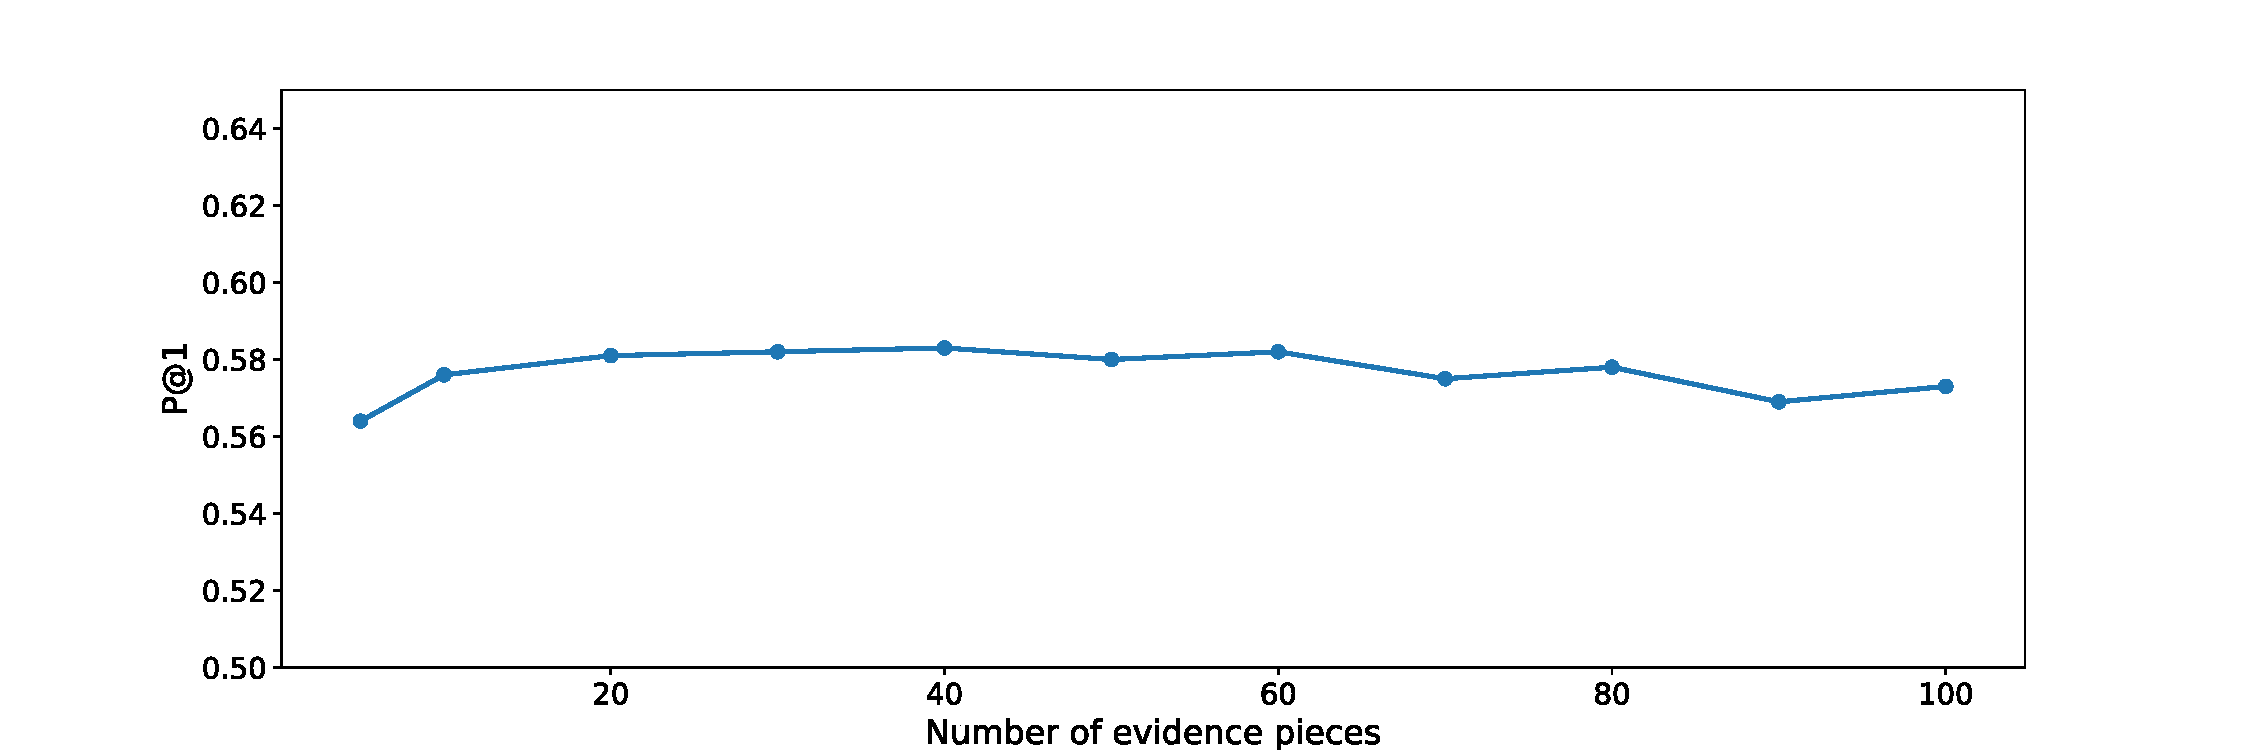
\includegraphics[width=0.8\textwidth]{submissions/Gerhard2024/figures/p_at_1-line_with_evidences.pdf}
    \vspace*{-0.2cm}
    \caption{Performance of \method on the \compmix dev set with different numbers of evidence.}
    \label{fig:res-num-evidences}
    \vspace*{-0.2cm}
\end{figure}



%%% ABLATION
\myparagraph{Ablation study on re-ranking} For more insight on the possible configurations of the RF stage, we conducted an ablation study with different options, including solely relying on the initial BM25 scoring without explicit re-ranking. The results are shown in Table \ref{tab:ablation2}. We observe that the iterative reduction in two steps is slightly better than the single-step variants (going down from top-1000 to top-30 in one RF step). Between the two options of using a GNN or a CE, the differences are negligible. A notable effect is that our RF techniques retain the answer presence at a very high level, only a bit lower than for the initial top-1000. 
The last two rows of Table \ref{tab:ablation2} demonstrate that RF is crucial: without explicit re-ranking, the technique of just picking smaller top-$k$ from the original BM25 model leads to substantial degradation in both answer presence and precision. 


\begin{table} [t] \small
    \centering
    \newcolumntype{G}{>{\columncolor [gray] {0.90}}c}
    \newcolumntype{H}{>{\setbox0=\hbox\bgroup}c<{\egroup}@{}}
    	\begin{tabular}{l G H G G G} 
        \toprule
            & \multicolumn{5}{G}{\textbf{\compmix} (dev set)} \\
        \midrule
            \textbf{RF Method $\downarrow$ / Metric $\rightarrow$} & \textbf{P@1} & \textbf{AP@1000} & \textbf{AP@100}  & \textbf{AP@30} & \textbf{MRR@100} \\ 
        \midrule
            \textbf{GNN: 1000 $\rightarrow$ 100 $\rightarrow$ 30}             &  $\mathbf{0.574}$  & $0.760$ &  $0.738$  &  $0.710$  &  $\mathbf{0.572}$  \\
            \textbf{CE: 1000 $\rightarrow$ 100 $\rightarrow$ 30}          &  $0.573$  & $0.760$  &   $\mathbf{0.740}$ &  $\mathbf{0.721}$   &  $0.553$   \\
        \midrule
            \textbf{GNN: 1000 $\rightarrow$ 30} &  $0.567$  & $?$  &   $n/a$ &  $0.710$   &  $0.567$   \\
         \textbf{CE: 1000 $\rightarrow$ 30} &  $0.570$  & $0.760$  &   $n/a$ &  $0.715$   &  $0.558$   \\
            \midrule
           \textbf{BM25: 100 (w/o GNN or CE)} &  $0.490$ & $0.760$  &  $0.652$  &  $n/a$  &  $0.259$ \\       
            \textbf{BM25: 30 (w/o GNN or CE)} &  $0.468$  & $0.760$  &  $n/a$ &  $0.534$   &  $0.259$   \\
            \bottomrule
    \end{tabular}
    \vspace*{-0.2cm}
    \caption{Ablation study for different RF strategies of \method on the \compmix dev set. The answer presence in the RF input with top-$1000$ evidence pieces is $0.760$.}
    \label{tab:ablation2}
\end{table}



\myparagraph{Quality of SI}
To assess the quality and robustness of the Structured Intents, we
inspected a sample of questions and their SIs.
Table~\ref{tab:question-SI-examples} gives three anecdotic examples.
We show SIs generated by \method, which makes use of the pre-existing collection from the \compmix benchmark for training.
This training data was obtained via different heuristics, 
which can be a limiting factor when user intents become more complex.

Therefore, we also looked at SIs derived via in-context learning (ICL) using \gptfour with $5$ handcrafted examples.
As shown in our earlier work on temporal QA~\cite{Jia-FAITH:WWW2024},
such data can be used for training smaller models (e.g., BART),
which can greatly boost the completeness and overall quality of the generated SIs.

From the sampled set, we observed that the ICL-based SIs are more
complete with all slots filled, whereas the BART-based SIs focused more
on the main slots Answer-type, Entities and Relation.
However, both approaches achieve very high quality in filling the slots,
capturing the user's information need very well.

Interestingly, when questions get complicated, with nested phrases, 
the ICL-based variant succeeds in decomposing the questions, based on only $5$ ICL examples.
For example, for the question {\em ``which German state had the most Corona-related death cases in the first year after the outbreak?''}
the Time slot becomes {\em ``first year after Corona outbreak''},
which can be resolved to identify the temporal scope.
In general, we believe that such question decomposition, beyond simple temporal constraints,
would be an interesting theme for future work.

\begin{table} [t] 
    \centering
    \small
    \newcolumntype{G}{>{\columncolor [gray] {0.90}}c}
    \newcolumntype{H}{>{\setbox0=\hbox\bgroup}c<{\egroup}@{}}
    \resizebox*{\textwidth}{!}{
        \begin{tabular}{p{6cm}|p{6cm}|p{6cm}} 
        \toprule
            \textbf{Question} & \textbf{Current SI by \method} & \textbf{SI via ICL} \\
        \midrule
        \textit{what was disneys first color movie?}
            & Ans-Type: \textit{animated feature film} & Ans-Type: \textit{film, animated film} \\
            & Entities: \textit{disneys} & Entities: \textit{Disney} \\
            & Relation: \textit{was first color movie} & Relation: \textit{first color movie} \\
            &  & Time: \textit{first} \\
        \midrule
        \textit{at the oscars, who won best actor in 2018?}
            & Ans-Type: \textit{human} & Ans-Type: \textit{person, actor} \\
            & Entities: \textit{at the oscars} & Entities: \textit{Oscars, 2018} \\
            & Relation: \textit{who won best actor in 2018} & Relation: \textit{won best actor} \\
            &  & Time: \textit{2018} \\
        \midrule
        \textit{which German state had the most Corona-} & Ans-Type: \textit{state} & Ans-Type: \textit{location, state} \\
        \textit{related death cases in the first year after} & Entities: \textit{Germany, Corona} & Entities: \textit{Germany, Corona-related deaths} \\
        \textit{the outbreak?} & Relation: \textit{which state had the most related} & Relation: \textit{highest count of death cases} \\
        & \textit{death cases in the first year after the out-}  & Location: \textit{Germany} \\
            & \textit{break}  & Time: \textit{first year after Corona outbreak} \\
        \bottomrule
    \end{tabular}
    }
    \vspace*{-0.2cm}
    \caption{Examples for pairs of question and generated SI.}
    \label{tab:question-SI-examples}
\end{table}




%%% REFRAIN FROM ANSWER
\myparagraph{Refraining from answering}
%%% Searched for: "generated_answer I" (with I being the full word, not partial) in the generated answers of LLaMA
%%% yields 245 results out of 2764 questions on CompMix
%%% yields 1270 results out of 3237 questions on TimeQuestions
We can train our model to refrain from answering in scenarios
where the provided evidence does not contain an answer to the question.
Specifically, during training, when the answer is not present in the evidence,
we change the target answer to {\em unknown}. This variant is referred to as \method {\em (faithful)}.

We measure the ratio of questions for which {\em unknown} is provided as answer,
and the P@1 restricted to questions that are answered.
The accuracy of refraining from answering is measured as well,
based on whether the answer is present in the evidence or not.
We conduct this experiment on \compmix and \timequestions,
for which we can compute answer presence exactly.
We also compute results for \llama, which is already instructed 
with the option to answer ``don't know''.
Table~\ref{tab:refrain-from-answer} shows the results.
For \compmix, we observe that \method has high accuracy on refraining when appropriate,
whereas \llama tends to be overconfident with a very small rate of {\em unknowns}, leading to incorrect answers.

\begin{table} [t] \small
    \centering
    \newcolumntype{G}{>{\columncolor [gray] {0.90}}c}
    \newcolumntype{H}{>{\setbox0=\hbox\bgroup}c<{\egroup}@{}}
    	\begin{tabular}{l G G G G c c c c} 
        \toprule
            & \multicolumn{4}{G}{\textbf{\compmix}} & \multicolumn{4}{c}{\textbf{\timequestions}} \\
            \midrule
            \textbf{Metric $\rightarrow$} & \textbf{P@1}  & \textbf{P@1} & \textbf{Refrain} & \textbf{Refrain} & \textbf{P@1}  & \textbf{P@1} & \textbf{Refrain} & \textbf{Refrain} \\ 
            \textbf{Method $\downarrow$} &                 & \textbf{(answered)} & \textbf{rate} & \textbf{accuracy} &                 & \textbf{(answered)} & \textbf{rate} & \textbf{accuracy} \\ 
            \midrule
                \textbf{\llama}             &  $0.431$  &  $0.471$  &  $0.089$  &  $n/a$  &  $0.177$  &  $0.276$  &  $0.392$  &  $n/a$  \\
                \textbf{\method (faithful)}           &  $0.497$  &  $0.713$  &  $0.303$  &  $0.838$ &  $0.597$  &  $0.804$  &  $0.257$  &  $0.864$  \\
            \bottomrule
    \end{tabular}
    \vspace*{-0.2cm}
    \caption{
        Performance of \method with option to refrain from answering (``don't know'').
    }
    \label{tab:refrain-from-answer}
\end{table}

\label{sec:disc}
\section{Insights, Limitations, and Challenges}


\noindent{\bf Benchmark Performance.} Our method, RAG-based \method with an 8B LLaMA model, outperforms much larger LLMs like \gptfour on two of the three benchmarks, with a very large margin for temporal questions. Obviously, pre-trained LLMs have only limited sense of properly positioning ``remembered’’ facts on the timeline even with training data that exceeds ours by several orders of magnitude. This confirms our intuition that LLMs alone are not good at ``recalling’’  higher-arity relations that require combining distant pieces of evidence. This is a sweet spot for RAG. Only for 
the \crag benchmark, \method is substantially inferior to a full-blown LLM. This is likely due to the nature of the questions: not necessarily the complexity of the information needs, but the need for more web sources (beyond what our experiments tap into).

\vspace{0.2cm}
\noindent{\bf Cost/Performance Ratio.} The most important take-away from our experiments is that \method achieves its competitive performance at a much lower cost than the full LLMs. Assuming that the consumed GFlops are proportional to the number of model parameters, \method achieves a cost reduction by a factor of 200x for \gptthree and 2000x for \gptfour. This does not only mean less computation, but also a massively lower electricity bill and climate impact.  

\vspace{0.2cm}
\noindent{\bf Role of Question Understanding.} We did not systematically investigate the influence of the Structured Intent in the \method pipeline. However, the comparison to the big GPT models reflects the role of the SI, as we prompt the GPT models in their natural mode with the original questions. The linearized sequence of available SI slots does not always have major advantages, but there are enough cases where specific facets provide crucial cues. This holds especially for the Entities slot, as this drives the gathering of evidence in the ER stage (cf.~\cite{Christmann-CONVINSE:SIGIR2022}, and for the Time slot, as these cues are often decisive for temporal questions (cf.~\cite{Jia-FAITH:WWW2024}).

\vspace{0.2cm}
\noindent{\bf Role of Re-Ranking.} As our ablation studies show, merely using top-$k$ evidence from an initial BM25-style ranking does not provide good performance. Also, there seems to be sweet spot in the choice of $k$: we need enough evidence for connecting the dots if the question requires multiple pieces of information, or for corroborating candidates if the question finds many useful but noisy pieces. In the experiments, $k=30$ turns out to be good choice; much lower $k$ results in insufficient evidence, and much larger $k$ leads to saturation and ultimately degrading performance. Our argument for iteratively shrinking the candidate set in multiple rounds of re-ranking is substantiated in our experiments, but the gain of doing this, compared to GNN- or CE-based re-ranking from 1000 to 30, is not big. More research is called to better understand the role of ranking in RAG. 

\vspace{0.2cm}
\noindent{\bf Limitations of Evidence Retrieval.}
For ER, we adopted more or less standard techniques. The results showed very good answer presence, in the order of 75\% in the top-100 or even top-30. An important case where this is insufficient are questions that require aggregating information over a large number of evidence pieces. An example is asking for the life-time total of 3-point scores of the basketball player Dirk Nowitzki.
This requires collecting a set of per-season tables with NBA player statistics, but also other web sources with numbers for his career before he joined the NBA (including his youth teams).
Of course, there are sometimes shortcuts like a Wikipedia article or biography mentioning the total number, but this cannot be universally assumed. The bottom line is that ER should be reconsidered as well, striving to improve the recall dimension.

\vspace{0.2cm}
\noindent{\bf Limitations of Answer Generation.}
For AG, we simply rely on a LLM,
using it as an extractor (``reader'') from the given evidence. Despite the wide belief that LLMs can perform deep
reasoning over many pieces of evidence, our experience is that the extraction works only well – robustly and faithfully – for relatively simple questions with a few multi-hop joins or simple aggregation over a few pieces. However, complicated questions such as asking for the top-100 NBA players with the largest number of life-time 3-point scores (again including their pre-NBA careers) are currently out of scope and will likely remain so for quite some time. This offers many opportunities for pushing the envelope further.

\vspace{0.2cm}
\noindent{\bf Trust in Data Sources.}
In our experiments, we considered all heterogeneous sources as trustworthy and unbiased. With focus on Wikidata and Wikipedia, this assumption has been well justified. In the wild, however, input data for RAG-based systems likely exhibit a wide spectrum of quality issues, in terms of stale information, biased positions, or simply false statements. Identifying trustworthy and up-to-date evidence and dealing with conflicting data, has been explored in other contexts (e.g., for KG curation~\cite{Dong-Trust:PVLDB2015}), but remains a major challenge for RAG-based QA.


\vspace{0.2cm}
\noindent{\bf Open Challenges and Future Work.} The best-performing methods in our experiment, mostly \method, reach P@1 values of 56\% for \compmix and 75\% for \timequestions. 
For the latter, the answer presence in the top-100 is only slightly higher; so the AG stage hardly misses anything.
However, for \compmix, the answer presence is 75\% -- much higher than what our system can actually answer. Obviously, closing this gap is a major direction to pursue, with focus on the RF and AG stages. However, missing one fourth of the answers completely in the top-100 pool, is a big problem as well. This requires improving recall at the ER stage, possibly with better guidance by the QU, which in turn needs more sources beyond the scope of our experiments (currently limited to Wikidata and Wikipedia). 

In general, we need to think beyond this kind of ``benchmark mindset’’. Even if we reached 80\% or 90\% precision and recall, we would still have a substantial fraction of questions that are answered incorrectly
or not at all. 
The remaining errors may not be a problem for chatbots, but they would be a showstopper for the deployment of mission-critical applications in business or science. We believe that this big gap is a shortcoming of {\em all methods}, not an issue that comes from the data alone. For trivia-style QA, as looked at in this paper, a smart human in ``open book’’ mode and no time limitation should be able to properly answer practically all questions, just by reading pieces of web contents and putting things together. Neither LLMs nor state-of-the-art RAG are the final solution; substantial research and creative ideas are needed to further advance QA.


\clearpage
\newpage

\newcommand{\bibauthors}[1]{{#1}}
\newcommand{\bibtitle}[1]{\emph{#1}}
\newcommand{\bibconf}[1]{{#1}}

\begin{thebibliography}{10}

\bibitem{Bajaj:arxiv2018}
\bibauthors{Payal Bajaj, Daniel Campos, Nick Craswell, Li Deng, Jianfeng Gao, Xiaodong Liu, Rangan Majumder, Andrew McNamara, Bhaskar Mitra, Tri Nguyen, Mir Rosenberg, Xia Song, Alina Stoica, Saurabh Tiwary, Tong Wang.}
\bibtitle{MS MARCO: A Human Generated MAchine Reading COmprehension Dataset.}
In \bibconf{arXiv 2018}.

\bibitem{DBLP:conf/acl/ChenFWB17}
\bibauthors{Danqi Chen, Adam Fisch, Jason Weston and Antoine Bordes.}
\bibtitle{Reading Wikipedia to Answer Open-Domain Questions.}
In \bibconf{ACL 2017}.

\bibitem{Christmann-CONVINSE:SIGIR2022}
\bibauthors{Philipp Christmann, Rishiraj Saha Roy, Gerhard Weikum.}
\bibtitle{Conversational Question Answering on Heterogeneous Sources.}
In \bibconf{SIGIR 2022}.

\bibitem{Christmann-CLOCQ:WSDM2022}
\bibauthors{Philipp Christmann, Rishiraj Saha Roy, Gerhard Weikum.}
\bibtitle{Beyond NED: Fast and Effective Search Space Reduction for Complex Question Answering over Knowledge Bases.}
In \bibconf{WSDM 2022}.

\bibitem{Christmann-Explaignn:SIGIR2023}
\bibauthors{Philipp Christmann, Rishiraj Saha Roy, Gerhard Weikum.}
\bibtitle{Explainable Conversational Question Answering over Heterogeneous Sources via Iterative Graph Neural Networks.}
In \bibconf{SIGIR 2023}.

\bibitem{Christmann-CompMix:WWW2024}
\bibauthors{Philipp Christmann, Rishiraj Saha Roy, Gerhard Weikum.}
\bibtitle{CompMix: A Benchmark for Heterogeneous Question Answering.}
In \bibconf{WWW 2024}.

\bibitem{Dejean:arxiv2024}
\bibauthors{Herve Dejean, Stephane Clinchant, Thibault Formal.}
\bibtitle{A Thorough Comparison of Cross-Encoders and LLMs for Reranking SPLADE.}
In \bibconf{arXiv 2024}.

\bibitem{Dhingra-time-aware-LLM:TACL2022}
\bibauthors{Bhuwan Dhingra, Jeremy R Cole, Julian Martin Eisenschlos, Daniel Gillick, Jacob Eisenstein, and William W Cohen.}
\bibtitle{Time-Aware Language Models as Temporal Knowledge Bases.}
In \bibconf{TACL 2022}.

\bibitem{Dong-Trust:PVLDB2015}
\bibauthors{Xin Luna Dong, Evgeniy Gabrilovich, Kevin Murphy, Van Dang, Wilko Horn, Camillo Lugaresi, Shaohua Sun, Wei Zhang.}
\bibtitle{Knowledge-Based Trust: Estimating the Trustworthiness of Web Sources.}
In \bibconf{PVLDB 2015}.

\bibitem{DBLP:journals/arXiv/abs-2312-10997}
\bibauthors{Yunfan Gao, Yun Xiong, Xinyu Gao, Kangxiang Jia, Jinliu Pan, Yuxi Bi, Yi Dai, Jiawei Sun, Qianyu Guo, Meng Wang, Haofen Wang.}
\bibtitle{Retrieval-Augmented Generation for Large Language Models: A Survey.}
In \bibconf{arXiv 2023}.

\bibitem{Gao-citations:emnlp2023}
\bibauthors{Tianyu Gao, Howard Yen, Jiatong Yu, Danqi Chen.}
\bibtitle{Enabling Large Language Models to Generate Text with Citations.}
In \bibconf{EMNLP 2023}.

\bibitem{Guu-REALM:ICML2020}
\bibauthors{Kelvin Guu, Kenton Lee, Zora Tung, Panupong Pasupat, Ming-Wei Chang.}
\bibtitle{Retrieval Augmented Language Model Pre-Training.}
In \bibconf{ICML 2020}.

\bibitem{DBLP:conf/eacl/IzacardG21}
\bibauthors{Gautier Izacard, Edouard Grave.}
\bibtitle{Leveraging Passage Retrieval with Generative Models for Open Domain Question Answering.}
In \bibconf{EACL 2021}.

\bibitem{Jia-TimeQuestions}
\bibauthors{Zhen Jia, Soumajit Pramanik, Rishiraj Saha Roy, and Gerhard Weikum.}
\bibtitle{Complex Temporal Question Answering on Knowledge Graphs.}
In \bibconf{CIKM 2021}.

\bibitem{Jia-FAITH:WWW2024}
\bibauthors{Zhen Jia, Philipp Christmann, Gerhard Weikum.}
\bibtitle{Faithful Temporal Question Answering over Heterogeneous Sources.}
In \bibconf{WWW 2024}.

\bibitem{DBLP:journals/arXiv/abs-2305-06984}
\bibauthors{Ehsan Kamalloo, Nouha Dziri, Charles L. A. Clarke, Davood Rafiei.}
\bibtitle{Evaluating Open-Domain Question Answering in the Era of Large Language Models.}
In \bibconf{arXiv 2023}.

\bibitem{Kandpal:ICML2023}
\bibauthors{Nikhil Kandpal, Haikang Deng, Adam Roberts, Eric Wallace, Colin Raffel.}
\bibtitle{Large Language Models Struggle to Learn Long-Tail Knowledge.}
In \bibconf{ICML 2023}.

\bibitem{DBLP:conf/emnlp/KarpukhinOMLWEC20}
\bibauthors{Vladimir Karpukhin, Barlas Oguz, Sewon Min, Patrick S. H. Lewis, Ledell Wu, Sergey Edunov, Danqi Chen, Wen-tau Yih.}
\bibtitle{Dense Passage Retrieval for Open-Domain Question Answering.}
In \bibconf{EMNLP 2020}.

\bibitem{Lee-MATTER:ACL2024}
\bibauthors{Dongkyu Lee, Chandana Satya Prakash, Jack FitzGerald, Jens Lehmann.}
\bibtitle{MATTER: Memory-Augmented Transformer Using Heterogeneous Knowledge Sources.}
In \bibconf{ACL 2024}.

\bibitem{DBLP:conf/acl/LewisLGGMLSZ20}
\bibauthors{Mike Lewis, Yinhan Liu, Naman Goyal, Marjan Ghazvininejad, Abdelrahman Mohamed, Omer Levy, Veselin Stoyanov, Luke Zettlemoyer.}
\bibtitle{BART: Denoising Sequence-to-Sequence Pre-training for Natural Language Generation, Translation, and Comprehension.}
In \bibconf{ACL 2020}.

\bibitem{DBLP:conf/nips/LewisPPPKGKLYR020}
\bibauthors{Patrick S. H. Lewis, Ethan Perez, Aleksandra Piktus, Fabio Petroni, Vladimir Karpukhin, Naman Goyal, Heinrich Küttler, Mike Lewis, Wen-tau Yih, Tim Rocktäschel, Sebastian Riedel, Douwe Kiela.}
\bibtitle{Retrieval-Augmented Generation for Knowledge-Intensive NLP Tasks.}
In \bibconf{NeurIPS 2020}.

\bibitem{Lin:MC2021}
\bibauthors{Jimmy Lin, Rodrigo Frassetto Nogueira, Andrew Yates.}
\bibtitle{Pretrained Transformers for Text Ranking: BERT and Beyond.}
In \bibconf{Morgan \& Claypool Publishers 2021}.

\bibitem{Liu-SUQL:NAACL2024}
\bibauthors{Shicheng Liu, Jialiang Xu, Wesley Tjangnaka, Sina J. Semnani, Chen Jie Yu, Monica Lam.}
\bibtitle{SUQL: Conversational Search over Structured and Unstructured Data with Large Language Models.}
In \bibconf{NAACL-HLT 2024}.

\bibitem{Mavi:FnT2024}
\bibauthors{Vaibhav Mavi, Anubhav Jangra, Adam Jatowt.}
\bibtitle{Multi-hop Question Answering.}
In \bibconf{Foundations and Trends in Information Retrieval 2024}.

\bibitem{Minaee-LLM-survey}
\bibauthors{Shervin Minaee, Tomas Mikolov, Narjes Nikzad, Meysam Chenaghlu, Richard}
\bibtitle{Socher, Xavier Amatriain, and Jianfeng Gao.}
Large Language Models: A Survey.
In \bibconf{arXiv 2024}.

\bibitem{Nogueira:arxiv2019}
\bibauthors{Rodrigo Frassetto Nogueira, Kyunghyun Cho.}
\bibtitle{Passage Re-ranking with BERT.}
In \bibconf{arXiv 2019}.

\bibitem{Oguz-UniK-QA:NAACL2022}
\bibauthors{Barlas Oguz, Xilun Chen, Vladimir Karpukhin, Stan Peshterliev, Dmytro Okhonko, Michael Sejr Schlichtkrull, Sonal Gupta, Yashar Mehdad, Scott Yih.}
\bibtitle{UniK-QA: Unified Representations of Structured and Unstructured Knowledge for Open-Domain Question Answering.}
In \bibconf{NAACL-HLT 2022}.

\bibitem{RogersGA:CS2023}
\bibauthors{Anna Rogers, Matt Gardner, Isabelle Augenstein.}
\bibtitle{QA Dataset Explosion: A Taxonomy of NLP Resources for Question Answering and Reading Comprehension.}
In \bibconf{ACM Computing Surveys 2023}.

\bibitem{RoyAnand:MC2021}
\bibauthors{Rishiraj Saha Roy, Avishek Anand.}
\bibtitle{Question Answering for the Curated Web: Tasks and Methods in QA over Knowledge Bases and Text Collections.}
In \bibconf{Synthesis Lectures on Information Concepts, Retrieval, and Services, Morgan \& Claypool Publishers 2021}.

\bibitem{Pramanik-Uniqorn:JWS2024}
\bibauthors{Soumajit Pramanik, Jesujoba Alabi, Rishiraj Saha Roy, Gerhard Weikum.}
\bibtitle{UNIQORN: Unified Question Answering over RDF Knowledge Graphs and Natural Language Text.}
In \bibconf{Journal of Web Semantics 2024}.

\bibitem{Sun-PullNet:EMNLP2019}
\bibauthors{Haitian Sun, Tania Bedrax-Weiss, William W. Cohen.}
\bibtitle{PullNet: Open Domain Question Answering with Iterative Retrieval on Knowledge Bases and Text.}
In \bibconf{EMNLP/IJCNLP 2019}.

\bibitem{Sun:NAACL2024}
\bibauthors{Kai Sun, Yifan Ethan Xu, Hanwen Zha, Yue Liu, Xin Luna Dong.}
\bibtitle{Head-to-Tail: How Knowledgeable are Large Language Models (LLMs)? A.K.A. Will LLMs Replace Knowledge Graphs?}
In \bibconf{NAACL-HLT 2024}.

\bibitem{Touvron-LLaMA}
\bibauthors{Hugo Touvron, Thibaut Lavril, Gautier Izacard, Xavier Martinet, Marie-Anne Lachaux, Timothée Lacroix, Baptiste Rozière, Naman Goyal, Eric Hambro, Faisal Azhar, Aurelien Rodriguez, Armand Joulin, Edouard Grave, Guillaume Lample.}
\bibtitle{Llama: Open and efficient foundation language models.}
In \bibconf{arXiv 2023}.

\bibitem{Wu-STARK:arxiv2024}
\bibauthors{Shirley Wu, Shiyu Zhao, Michihiro Yasunaga, Kexin Huang, Kaidi Cao, Qian Huang, Vassilis N. Ioannidis, Karthik Subbian, James Zou, Jure Leskovec.}
\bibtitle{STaRK: Benchmarking LLM Retrieval on Textual and Relational Knowledge Bases.}
In \bibconf{arXiv 2024}.

\bibitem{Wu:IEEE2021}
\bibauthors{Zonghan Wu, Shirui Pan, Fengwen Chen, Guodong Long, Chengqi Zhang, Philip S. Yu.}
\bibtitle{A Comprehensive Survey on Graph Neural Networks.}
In \bibconf{IEEE Transactions on Neural Networks and Learning Systems 2021}.

\bibitem{Yang-CRAG}
\bibauthors{Xiao Yang, Kai Sun, Hao Xin, Yushi Sun, Nikita Bhalla, Xiangsen Chen, Sajal Choudhary, Rongze D. Gui, Ziran W. Jiang, Ziyu Jiang, Lingkun Kong, Brian Moran, Jiaqi Wang, Yifan Ethan Xu, An Yan, Chenyu Yang, Eting Yuan, Hanwen Zha, Nan Tang, Lei Chen, Nicolas Scheffer, Yue Liu, Nirav Shah, Rakesh Wanga, Anuj Kumar, Wen-tau Yih, Xin Luna Dong.}
\bibtitle{CRAG -- Comprehensive RAG Benchmark.}
In \bibconf{arXiv 2024}.

\bibitem{Yasunaga:NAACL2021}
\bibauthors{Michihiro Yasunaga, Hongyu Ren, Antoine Bosselut, Percy Liang, Jure Leskovec.}
\bibtitle{QA-GNN: Reasoning with Language Models and Knowledge Graphs for Question Answering.}
In \bibconf{NAACL-HLT 2021}.

\bibitem{Zhang-Spaghetti:ACL2024}
\bibauthors{Heidi C. Zhang, Sina J. Semnani, Farhad Ghassemi, Jialiang Xu, Shicheng Liu, Monica S. Lam.}
\bibtitle{SPAGHETTI: Open-Domain Question Answering from Heterogeneous Data Sources with Retrieval and Semantic Parsing.}
In \bibconf{ACL 2024}.

\bibitem{Zhang:NAACL2024}
\bibauthors{Jiahao Zhang, Haiyang Zhang, Dongmei Zhang, Yong Liu, Shen Huang.}
\bibtitle{End-to-End Beam Retrieval for Multi-Hop Question Answering.}
In \bibconf{NAACL-HLT 2024}.

\bibitem{Zhao-LLMsurvey}
\bibauthors{Wayne Xin Zhao, Kun Zhou, Junyi Li, Tianyi Tang, Xiaolei Wang, Yupeng Hou, Yingqian Min, Beichen Zhang, Junjie Zhang, Zican Dong, Yifan Du, Chen Yang, Yushuo Chen, Zhipeng Chen, Jinhao Jiang, Ruiyang Ren, Yifan Li, Xinyu Tang, Zikang Liu, Peiyu Liu, Jian-Yun Nie, Ji-Rong Wen.}
\bibtitle{A Survey of Large Language Models.}
In \bibconf{arXiv 2023}.

\bibitem{Zhao:arxiv2024}
\bibauthors{Penghao Zhao, Hailin Zhang, Qinhan Yu, Zhengren Wang, Yunteng Geng, Fangcheng Fu, Ling Yang, Wentao Zhang, Bin Cui.}
\bibtitle{Retrieval-Augmented Generation for AI-Generated Content: A Survey.}
In \bibconf{arXiv 2024}.

\bibitem{Zhu-ODQA-survey:arxiv2021}
\bibauthors{Fengbin Zhu, Wenqiang Lei, Chao Wang, Jianming Zheng, Soujanya Poria, Tat-Seng Chua.}
\bibtitle{Retrieving and Reading: A Comprehensive Survey on Open-domain Question Answering.}
In \bibconf{arXiv 2021}.

\end{thebibliography}


\end{document}

\end{article}
\begin{article}
{Bringing Order to Chaos: Conceptualizing a Personal Research Knowledge Graph for Scientists}
{Prantika Chakraborty, Sudakshina Dutta, Debarshi Kumar Sanyal, Srijoni Majumdar, Partha Pratim Das}
\setcounter{section}{0}
\documentclass{article}

\usepackage{deauthor}

\usepackage{latexsym}
\usepackage{graphicx}
\graphicspath{{./images/}}
\usepackage{booktabs} % for formal tables
\usepackage{color}  % for coloring text
\usepackage{amsmath}  % for aligning equations
\usepackage{subcaption}
\usepackage{caption}
\usepackage{tikz}
\usepackage{colortbl} % for color in tables
\usepackage{framed}
\usepackage{multirow}
\usepackage{multicol}
\usepackage{hyperref}
\usepackage{url}
\usepackage{balance}
\usepackage{verbatim}
\usepackage{cancel}
\usepackage{xspace} % for correcting space after macro commands
\usepackage{algorithm2e}
\usepackage{bbold} % for writing mathbb{1}
\usepackage{balance}
\usepackage{stmaryrd}
\usepackage{enumitem}
\usepackage{array} % package for hiding a column
\usepackage{bold-extra} % to enable textbf with textsc

% used for making text readable in document and .tex
% \setlength{\parindent}{0pt}

\newcommand{\struct}[1]{\texttt{\small #1}}
\newcommand{\utterance}[1]{\textit{#1}}
\newcommand{\phrase}[1]{\textit{``#1''}}

% \newcommand {\g}[1]{\textcolor[gray]{0.6}{#1}}

\newcommand{\drop}{\dag\xspace}

\newenvironment{Snugshade}[1][236,236,236]{
    \setlength{\itemsep}{0pt}
     \setlength{\parsep}{0pt}
     \setlength{\topsep}{0pt}
     \setlength{\partopsep}{0pt}
     \setlength{\leftmargin}{1.5em}
     \setlength{\labelwidth}{0em}
     \setlength{\labelsep}{0em} 
    \setlength{\parskip}{0pt}
    \definecolor{shadecolor}{RGB}{#1}
    \begin{snugshade}
}{
    \end{snugshade}
}


\newcommand{\method}{\textsc{Quasar}\xspace}
\newcommand{\benchmark}{\textsc{PerQA}\xspace}
\newcommand{\itemslist}[1]{$\langle$\struct{#1}$\rangle$}


\newcommand{\convinse}{\textsc{Convinse}\xspace}
\newcommand{\explaignn}{\textsc{Explaignn}\xspace}
\newcommand{\clocq}{\textsc{Clocq}\xspace}
\newcommand{\unikqa}{\textsc{UniK-Qa}\xspace}
\newcommand{\gptthree}{\textsc{Gpt-3}\xspace}
\newcommand{\gptfour}{\textsc{Gpt-4}\xspace}
\newcommand{\llama}{\textsc{Llama3}\xspace}
\newcommand{\spaghetti}{\textsc{Spaghetti}\xspace}


\newcommand{\compmix}{\textsc{CompMix}\xspace}
\newcommand{\timequestions}{\textsc{TimeQuestions}\xspace}
\newcommand{\crag}{\textsc{Crag}\xspace}


\newcommand{\squishlist}{
    \begin{list}{$\bullet$}{
        \setlength{\itemsep}{0pt}
	\setlength{\parsep}{3pt}
	\setlength{\topsep}{3pt}
	\setlength{\partopsep}{0pt}
	\setlength{\leftmargin}{1.5em}
	\setlength{\labelwidth}{1em}
	\setlength{\labelsep}{0.5em}
    }
}

\newcommand{\squishend}{
    \end{list}
}

\newcommand{\myparagraph}[1]{\vspace*{0.2cm}\noindent \textbf{#1}.}
\newcommand{\myparagraphnospace}[1]{\noindent \textbf{#1}.}

% \newcommand{\GW}[1]{\emph{{\color{blue} GW:#1}}}
% \newcommand{\PC}[1]{\emph{{\color{orange} PC: #1}}}
% \newcommand{\tocite}{{{\color{red} [CITE]}}}


\begin{document}

\title{RAG-based Question Answering \\ over Heterogeneous Data and Text}

\author{
Philipp Christmann,
Gerhard Weikum\\\\
Max Planck Institute for Informatics\\
Saarland Informatics Campus, Germany\\
\texttt{\{pchristm, weikum\}@mpi-inf.mpg.de}}

\maketitle

\section*{Abstract}
This article presents the \method system for question answering over unstructured text, structured tables, and knowledge graphs, with unified treatment of all sources.
The system adopts a RAG-based architecture, with a pipeline of evidence retrieval followed by answer generation, with the latter powered by a 
moderate-sized
language model.
Additionally and uniquely, \method
has components for question understanding, to derive crisper input for evidence retrieval, and for re-ranking and filtering the retrieved evidence before feeding the most informative pieces into the answer generation.
Experiments with three different benchmarks demonstrate the high answering quality of our approach, being on par with or better than large GPT models, while keeping the computational cost and energy consumption orders of magnitude lower.

\label{sec:intro}
\section{Introduction}

\noindent\textbf{Motivation and Problem.} The task of question answering, QA for short, arises in many flavors: factual vs. opinions, simple lookups vs. multi-hop inference, single answer vs. list of entities, 
direct answers vs. long-form, one-shot questions vs. conversations, and other varieties 
(see, e.g., surveys~\cite{RogersGA:CS2023,RoyAnand:MC2021}).
The state-of-the-art for this entire spectrum has been greatly advanced in the past decade. Most notably, incorporating deep learning into retriever-reader architectures (e.g.,~\cite{DBLP:conf/acl/ChenFWB17,DBLP:conf/eacl/IzacardG21,DBLP:conf/emnlp/KarpukhinOMLWEC20}) has boosted answering quality, and most recently, large language models (LLM)~\cite{Minaee-LLM-survey,Zhao-LLMsurvey} have pushed the envelope even further (e.g.,~\cite{DBLP:journals/arXiv/abs-2305-06984}).

% strengths and limitations of LLM for QA
Today’s LLMs alone are capable of accurately answering many \textit{factoid} questions, simply from their pre-trained parametric memory which latently encodes huge text corpora and other online contents.
However, this critically depends on the frequency of evidence in the underlying contents and the complexity of the information need. 
For example, 
asking for the {\em MVP of the 2024 NBA season} would easily return the correct answer Nikola Jokic, 
but asking for the {\em highest-scoring German NBA player} or the {\em MVP of the 2024 German basketball league} pose a big challenge.
The reason is that LLMs alone do not easily recall information about not so popular or even long-tail entities~\cite{Kandpal:ICML2023,Sun:NAACL2024},
and that they are mainly geared for direct look-ups as opposed to connecting multiple pieces of evidence~\cite{Mavi:FnT2024,Zhang:NAACL2024}.

% introduce RAG and discuss need for heterogeneous sources
\cite{DBLP:journals/arXiv/abs-2312-10997,Guu-REALM:ICML2020,DBLP:conf/nips/LewisPPPKGKLYR020,Zhao:arxiv2024}
known as RAG, address these bottlenecks. In addition to cleverly crafted prompts and few-shot examples, the LLM is provided with the top-ranked results of an explicit retrieval step, like web search or knowledge graph (KG) lookups. The former is often necessary for freshness of answers, and the latter may help with long-tail entities and also mitigate the notorious risk of hallucinations. Still, this generation’s RAG architectures are limited in how broad and how deep they tap into external sources. Popular AI assistants like Gemini or ChatGPT seem to primarily retrieve from the text of web pages (incl. Wikipedia articles), and academic research has additionally pursued knowledge augmentation by enhancing prompts with facts from large KGs (e.g., Wikidata).

An additional content modality that is still underexplored are {\em online tables}: a wide range of tabular data including HTML tables in web pages, spreadsheets and statistics, all the way to CSV and JSON datasets that are abundant on the Internet. There is prior work on joint support for text and KGs and for text and tables, but very little on all of these together -- some notable exceptions being~\cite{Christmann-CONVINSE:SIGIR2022,Christmann-Explaignn:SIGIR2023,Oguz-UniK-QA:NAACL2022,Zhang-Spaghetti:ACL2024}.


\noindent\textbf{Examples.} All three heterogeneous types of sources are crucial not only for answering different questions from different kinds of evidence, but also for combining multiple pieces of evidence of different modalities to infer correct and complete answers.
To 
illustrate
the need for tapping all sources, consider the following questions:

% \vspace*{0.2cm}
\begin{quote}
$Q1$: \utterance{Which Chinese basketballers have played in the NBA?}\\
 \indent $Q2$: \utterance{Who was the first Chinese NBA player?}\\
  \indent $Q3$: \utterance{Which Chinese NBA player has the most matches?}
\end{quote}
% \vspace*{0.2cm}

Q1 can be cast into querying a KG, but the list there is not necessarily complete and up-to-date, so additional evidence from text or tables would be desired. 
Q2 needs information about who played in which seasons, found only in web pages or sports-statistics tables. 
Finally, Q3 may be lucky in finding prominent textual evidence (e.g., in biographies, Wikipedia etc.), but this often faces divergent statements, and resolving contradictions needs to dive into more evidence. Besides, when textual evidence is rare and hard to find or not trustworthy enough, then information from multiple tables and text snippets may have to be aggregated (e.g., totals of per-season counts).
Some of this may perhaps become feasible for an industrial LLM’s RAG capabilities in the near future, but there are always harder scenarios by moving from Chinese NBA players deeper into the long tail, such as asking for {\em Lithuanian players in the German handball league}.

\vspace*{0.2cm}
\noindent\textbf{Approach and Contribution.} This paper presents a simple but powerful and versatile RAG system with unified access to text, KG and tables. We call our method {\em \method} 
(for Question Answering over Heterogeneous Sources with Augmented Retrieval).
Its architecture is relatively straightforward: all heterogeneous content is verbalized and indexed for retrieval; a retriever finds top-ranked results for the given question (from different source types), and these are fed into the LLM for answer generation. This is the unsurprising bird-eye’s view. Specific details that are key factors for the strong performance of \method are: 

\squishlist
\item[i)] automatically casting user questions into a structured representation of the information need, which is then used to guide 
\item[ii)] judicious ranking of search results, with multiple rounds of re-ranking and pruning, followed by
\item[iii)]	extracting faithful answers from an LLM in RAG mode, with answers grounded in tangible evidence.
\squishend


\vspace{0.2cm}
\noindent The paper presents experiments with three different benchmarks, covering various flavors of questions.
We focus on one-shot questions; conversational QA is out of scope here, but \method itself is well applicable to this case, too.
Our experiments demonstrate that our methods are competitive, on par with big GPT models and often better,
while being several orders of magnitude lower in computational and energy cost.
The experimental findings also highlight that question understanding, with structured representation of user intents, and iterative re-ranking of evidence are crucial for good performance.

Overall, our contribution lies in proposing a unified system architecture for RAG-based question answering over a suite of different data sources, with strong points regarding both effectiveness (i.e., answer quality)
and efficiency (i.e., computational cost).


\label{sec:background}
\section{Related Work}

The RAG paradigm came up as a principled way of enhancing LLM factuality incl. provenance and mitigating the risk of hallucination~\cite{Guu-REALM:ICML2020, DBLP:conf/nips/LewisPPPKGKLYR020}.
It is highly related to the earlier
retriever-reader architectures for QA~\cite{DBLP:conf/acl/ChenFWB17,DBLP:conf/emnlp/KarpukhinOMLWEC20}, especially when the reader uses the fusion-in-decoder method~\cite{DBLP:conf/eacl/IzacardG21,Oguz-UniK-QA:NAACL2022}.
Since its invention, RAG methodology has been greatly advanced, introducing a wide suite of extensions, such as batched inputs, interleaving retrieval and generation steps, and more (see the recent surveys~\cite{DBLP:journals/arXiv/abs-2312-10997,Zhao:arxiv2024}).

On question answering (QA), there is a vast amount of literature including a wealth of differently flavored benchmarks (see, e.g.,~\cite{RogersGA:CS2023}).
The case of interest here is QA over heterogeneous sources, tapping into both unstructured content and structured data. 
A variety of works has pursued this theme by combining knowledge graphs with text sources, using graph-based methods, neural learning and  language models (e.g.,~\cite{Pramanik-Uniqorn:JWS2024,Sun-PullNet:EMNLP2019,Yasunaga:NAACL2021}).

Most relevant for this article is the research on jointly leveraging all different sources: text, KGs, and tables (incl. CSV and JSON files). This includes  
the \unikqa system~\cite{Oguz-UniK-QA:NAACL2022},
the \spaghetti/SUQL project~\cite{Liu-SUQL:NAACL2024,Zhang-Spaghetti:ACL2024},
the \textsc{Matter} method~\cite{Lee-MATTER:ACL2024},
the STaRK benchmarking~\cite{Wu-STARK:arxiv2024},
and our own prior work
~\cite{Christmann-CONVINSE:SIGIR2022,Christmann-Explaignn:SIGIR2023} (without claiming exhaustiveness).
Out of these, we include \unikqa, \spaghetti and our own systems \convinse and \explaignn as baselines in the experimental evaluation.
Their architectures are similar to ours, but \unikqa and \spaghetti do not have our distinctive elements of
question understanding and iterative re-ranking (originally introduced in \explaignn~\cite{Christmann-Explaignn:SIGIR2023}).

\label{sec:method}
\section{Methodology}

\begin{figure}[tb]
  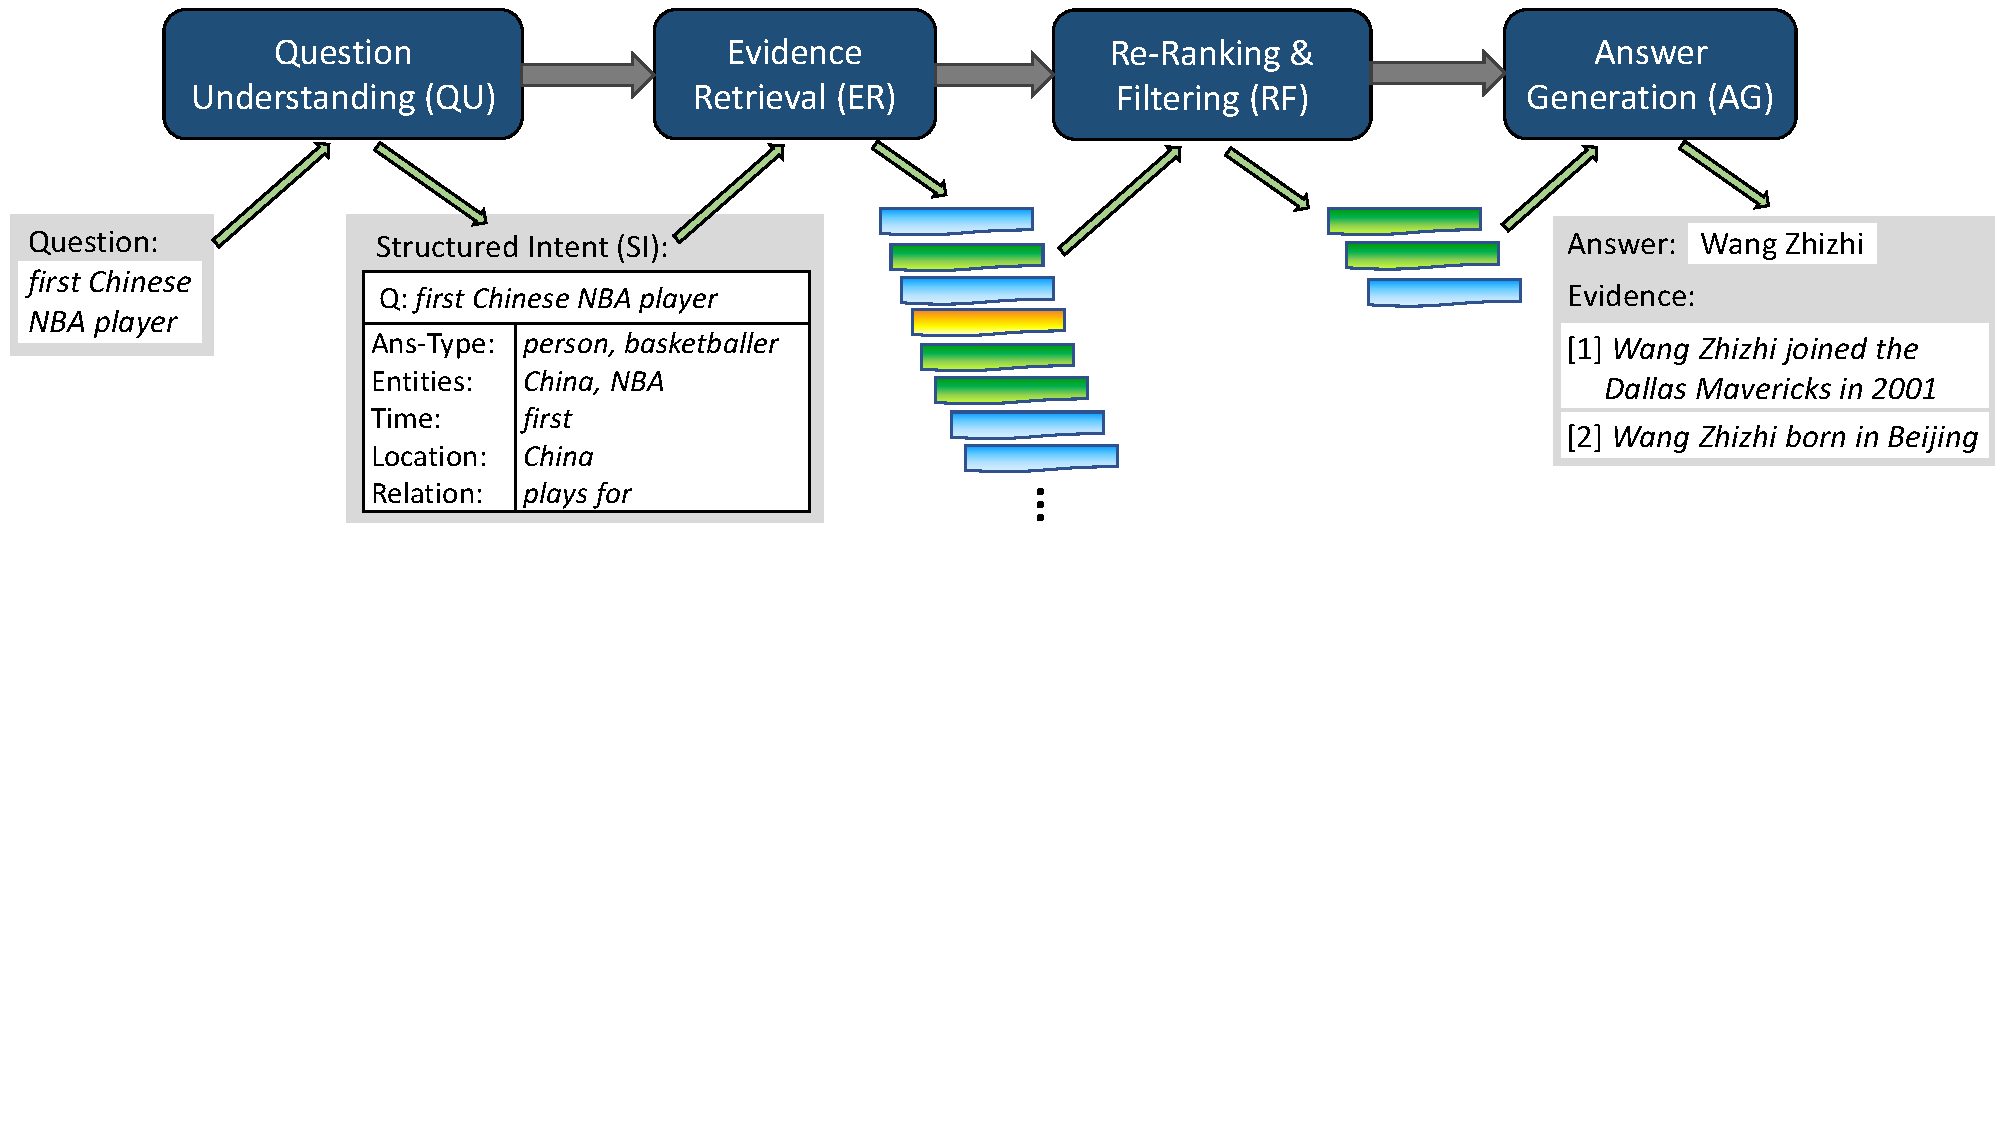
\includegraphics[width=\textwidth]{submissions/Gerhard2024/figures/compass-overview.pdf}
  \caption{Overview of the \method system.}
  \label{fig:compass-overview}
\end{figure}

% start with system overview
The \method system is a pipeline of four major stages, as illustrated in Figure \ref{fig:compass-overview}.
First, the input question is analyzed and decomposed, in order to compute a {\em structured intent (SI)} representation that will pass on to the subsequent steps, along with the original question. Second, the SI is utilized to retrieve pieces of evidence from different sources: text, KG and tables. 
Third, this pool of potentially useful evidence is filtered down, with iterative re-ranking, to arrive at a tractably small set of most promising evidence.
The final stage generates the answer from this evidence,
passing back the answer as well as evidence snippets for user-comprehensible explanation.

The second and fourth stage, Evidence Retrieval (ER) and Answer Generation (AG), are fairly standard. Such a two-phase architecture was called a retriever-reader architecture~\cite{Zhu-ODQA-survey:arxiv2021}. With a modern LLM replacing the earlier kinds of neural readers, this is the core of every RAG system~\cite{DBLP:journals/arXiv/abs-2312-10997}.

Stages 1 and 3 are unique elements of our architecture, judiciously introduced to improve both effectiveness (i.e., answer quality) and efficiency (i.e., computational cost).
Question Understanding (QU) provides the ER component with crisper and semantically refined input, and
the Re-Ranking \& Filtering (RF) stage is beneficial for
distilling the best evidence from the large pool of retrieved pieces.
The following subsections elaborate on the four stages of the pipeline, emphasizing the \method-specific steps QU and RF.



\subsection{Question Understanding (QU)}

% one par introducing the SI
To prepare the retrieval from different kinds of sources, including a KG, ad-hoc tables and text documents, it is useful to analyze and decompose the user question.
In this work, we aim to cast a question into a 
{\em structured intent (SI)} representation: essentially
a frame with faceted cues as slots, or equivalently, a concise set of key-value pairs. 
Figure \ref{fig:compass-overview} gives an idealized example for the question about the first Chinese NBA player. The facets or keys of potential interest here 
are:
\squishlist
\item {\em Ans-Type:} the expected answer type (or types when considering
different levels of semantic refinement), 
\item {\em Entities:} the salient entities in the question, and 
\item {\em Relation:} phrases that indicate which relation (between Q and A entities) the user is interested in. 
\squishend
\noindent In addition, as questions can have temporal or spatial aspects, the SI also foresees slots for:
\squishlist
\item {\em Time:} cues about answer-relevant time points or spans, including relative cues (e.g., ``before Covid'') and ordinal cues (e.g., ``first''), and
\item {\em Location:} cues about answer-relevant geo-locations.
\squishend

% discuss the spectrum of different SIs
\vspace{0.2cm}
\noindent The ideal SI for example question Q2 would look like:

\begin{quote}
{\em Ans-Type:} person, basketballer; {\em Entities:} China, NBA; {\em Time:} first;
{\em Location:} China; {\em Relation:} plays for.
\end{quote}

Note that the values for these slots can be crisp like entity names or dates, but they can also take the form of surface phrases. The SI purpose and value lie in the decomposition. In practice, many questions would only lead to a subset of faceted cues, leaving some slots empty. For the example in Figure \ref{fig:compass-overview}, an alternative SI could simply consist of

\begin{quote}
{\em Ans-Type:} person; {\em Entities:} China, NBA; {\em Time:} first.
\end{quote}

\noindent Even this simplified SI can be highly beneficial in guiding the subsequent evidence retrieval.

% sketch how an LM is trained to generate SIs 
To generate the SI from a user question, we employ a (small-scale) LM, specifically BART~\cite{DBLP:conf/acl/LewisLGGMLSZ20}, a Transformer-based auto-encoder with 140M parameters.\footnote{\url{https://huggingface.co/facebook/bart-base}}
BART is pre-trained for language representation; its power for our purpose comes from fine-tuning.
To this end, we generate (question, SI) pairs by using an instruction-trained LLM like GPT-4, with few-shot in-context learning (following our earlier work~\cite{Jia-FAITH:WWW2024}). 
Note that this is a one-time action; at inference-time we only use much smaller LMs.
The generated silver-standard pairs are then used to fine-tune BART.
In the experiments in this article, we leverage pre-existing collections of silver pairs, based on the training data of the CompMix benchmark~\cite{Christmann-CompMix:WWW2024}, 
comprising $3{,}400$ such pairs.


% outline value of SI for conversations
Although this paper focuses on single-shot questions, the \method architecture is also geared for conversational QA. In that setting, the SI can play an even bigger role, as (follow-up) questions are often formulated in a rather sloppy manner -- all but self-contained. For example, a conversation could start with a clear question {\em When did Wang Zhizhi join the NBA?}, followed a few dialog steps later, by a user utterance like {\em Which teams did he play for?} or simply {\em Which teams?}.
In such an informal conversation, the system needs to {\em contextualize} each user utterance based on the preceding turns in the dialog (e.g., inferring the relevant entities Wang Zhizhi and NBA from the conversational history).
For details on conversational QA, based on our architecture, see our earlier works~\cite{Christmann-CONVINSE:SIGIR2022,Christmann-Explaignn:SIGIR2023}.







%%%%%%%%%%%%%%%%%%%%%%%%%%%%%%%%%%%%%
\subsection{Evidence Retrieval (ER)}

The ER stage taps into a knowledge graph, a corpus of text documents, and a collection of web tables.
Specifically, for the experiments, we use the Wikidata KG,
all English Wikipedia articles, and all tables that are embedded in Wikipedia pages (incl. infoboxes, which can be seen as a special case of tables). 

% specifics: Clocq etc. - and the role of the SI
\vspace{0.2cm}
\noindent{\bf Retrieval from KG:}
To retrieve evidence from the KG, we utilize our earlier work
\clocq~\cite{Christmann-CLOCQ:WSDM2022}, which provides entity disambiguations and a relevant KG-subgraph for a given query.
Unlike most other works on QA-over-KG, \clocq fetches all KG-facts that are relevant for a given entity in a single step.
For example, when querying for
NBA players, it can traverse the KG neighborhood and pick up top teams, also considering so-called qualifier nodes in Wikidata which are often used for temporal scopes. 
As the disambiguation of entity names onto the KG can be tricky and noisy (e.g., China could be mapped to Chinese sports teams in all kinds of sports), \clocq considers several possible disambiguations~\cite{Christmann-CLOCQ:WSDM2022} (typically in the order of $10$ result entities).
The queries for \clocq are 
constructed by concatenating all slots of the question's SI.
For the example query about the first Chinese NBA player,
good result entities would be Dallas Mavericks, lists about NBA seasons, MVP awards etc., and their associated facts. These provide cues, but are likely insufficient to answer the question.


\vspace{0.2cm}
\noindent{\bf Retrieval from Text and Tables:}
The disambiguated entities returned by \clocq form anchors for tapping into text and tables.
\method first identifies 
relevant text documents and tables that refer to the anchor entities. With focus on Wikipedia, these are simply the articles for the respective entities. 
\method then constructs a keyword query that concatenates all available fields of the SI.
The query is evaluated against a linearized and verbalized representation (see below) of all sentences and all table rows in the selected documents.
This returns a set of sentences and 
and individual table rows, ranked by BM25 scores.


\vspace{0.2cm}
\noindent{\bf Evidence Verbalization:}
All results from the different data sources are uniformly treated by {\em linearizing} and {\em verbalizing} them
into token sequences. For KG results, the entity-centric triple sets are linearized via breadth-first traversal of the mini-graph starting from the entity node.
For tables, results are individual rows, which are contextualized by including labels from column headers and from the DOM-tree path of the article where the table comes from. For example, a table row about Wang Zhizhi playing for Dallas (Mavericks) in the 2000-2001 season, would be expressed as:

\vspace{0.05cm}
\hspace*{0.5cm} Wang Zhizhi / NBA Career / Season: 2000-2001, Team: Dallas, Games Played: 5 \dots
\vspace{0.05cm}

\noindent Finally, results from the text corpus are already in the form of token sequences, but we can additionally prefix these with the DOM-tree labels.
We can think of this entire pool of evidence as 
an on-the-fly corpus of potentially relevant pseudo-sentences, forming the input of the subsequent RF stage.


\vspace{0.2cm}
\noindent {\bf Result Ranking:}
Overall, the ER stage compiles a substantial set of evidence, possibly many thousands of entities, text snippets and table rows. Therefore, we practically restrict the pool to a subset of high-scoring pieces, like the top-$1000$.
For scoring, a simple BM25 model (a classical IR method) is applied. 
By default, we treat all evidence pieces uniformly with global scoring, no matter whether they come from KG, text or tables. 


\subsection{Re-Ranking and Filtering (RF)}

With a pool of top-$1000$ evidence pieces, we could invoke an LLM for answer generation. However, that would face a large fraction of noise (i.e., misleading evidence) and incur high costs of computation and energy consumption. 

For both of these reasons, we have devised light-weight techniques for iteratively reducing the top-$1000$ pieces to a small subset, say top-$30$ or top-$10$, that can be fed into an LLM at much lower cost (as LLM computations and pricing are at least linear in the number of input tokens). The difficulty is, of course, to do this without losing good evidence and reducing answer presence. Our techniques for this task are based on graph neural networks (GNNs)~\cite{Wu:IEEE2021} or cross-encoders (CEs)~\cite{Dejean:arxiv2024,Lin:MC2021}.

\myparagraph{GNN-based RF}
Given a large pool of evidence pieces from all sources, a bipartite graph is constructed:
\squishlist
\item {\em nodes} being evidence pieces or entities that occur in these pieces, and
\item {\em edges} connecting an evidence piece and an entity if the entity occurs in the evidence.
\squishend


The task for the GNN is to jointly score the evidence and the entity nodes in a multi-task learning setup. The latter are the {\em answer candidates}, and the evidence should give {\em faithful explanation} for an answer.
We build on our earlier work on explainable QA~\cite{Christmann-Explaignn:SIGIR2023}.

The node encodings are initialized with cross-encoder embeddings (see below) 
for node contents and the SI of the question. The inference iteratively adjusts the encodings based on message passing from neighboring nodes.
The GNN is trained via weak supervision from question-answer pairs:
evidence nodes are labeled as relevant if they are connected to
a gold answer.
More technical details are given in~\cite{Christmann-Explaignn:SIGIR2023}.

\method invokes the GNN in multiple rounds, iteratively reducing top-$k$ to top-$k^*$ nodes with $k^* \ll k$. In practice, we would typically consider two rounds: re-ranking top-$1000$ and pruning to top-100, and then reducing to top-30 or top-10, which are passed to the answer generation stage.
Note that this keeps the GNN at a tightly controlled size, so that its computational costs at inference-time are much smaller than those of an LLM.


\myparagraph{CE-based RF}
An alternative to the GNN inference is to employ a cross-encoder for scoring and re-ranking the evidence pieces.
These are transformers (typically with a small LM like BERT) that are fine-tuned for scoring the relatedness between a query and a document~\cite{Nogueira:arxiv2019}. In our case, the comparison is between the question SI and the evidence piece. In our experiments, we make use of two different cross-encoders, 
both trained on the MS-MARCO benchmark for passage retrieval~\cite{Bajaj:arxiv2018}, 
and fine-tuned on the respective benchmark (leveraging the same weak supervision data as for the GNNs),
the difference being in model size.\footnote{\url{https://huggingface.co/cross-encoder/ms-marco-MiniLM-L-4-v2} and\\ \url{https://huggingface.co/cross-encoder/ms-marco-MiniLM-L-6-v2}}
We use the smaller model to reduce top-$1000$ to top-100, and the larger model to go further down from top-100 to top-30.




%%%%%%%%%%%%%%%%%%%%%%%%%%%%%%%%%%%%%

\subsection{Answer Generation (AG)}

The last stage follows mainstream practice to invoke an LLM in a retrieval-augmented manner.
We call a `small-scale` LLM, specifically a fine-tuned LlaMA-3.1 model (8B-Instruct)\footnote{\url{https://huggingface.co/meta-llama/Llama-3.1-8B-Instruct}}, with a prompt \footnote{The specific prompt is \phrase{SI: \textless\texttt{concatenated SI}\textgreater \hspace{0.1cm} Evidence: \textless\texttt{evidence pieces}\textgreater}.}
consisting of:

\squishlist
\item the concatenated SI of the original question, and
\item the top-30 (or other top-$k^*$ with small $k^*$) evidence pieces.
\squishend

By the previous down-filtering of the original pool of evidence pieces, this last step has affordable cost in terms of computation time and energy consumption.

\vspace{0.2cm}
\noindent{\bf Fine-Tuning the LLM:}
We considered adding an instruction to the prompting, such as {\em ``answer this question solely based on the provided evidence snippets''}.
However, this turned out to be ineffective.
The reason why the model works well without such instructions is our task-specific fine-tuning.
We perform this by running the training data of benchmarks through the \method pipeline,
and training the AG stage with the top-30 evidence pieces as input.
Thus, the fine-tuning makes the model learn the role of evidence for RAG-based QA.

\vspace{0.2cm}
\noindent{\bf Explanations:}
The top-30 evidence pieces can be used to provide users with explanation of answers.
Optionally, these could be reduced further for comprehensibility.
Alternatively, we can fine-tune the LLM to provide both answers and concise explanations.
Since we can infer which evidences in the input mention the annotated ground-truth answers,
our method could be fine-tuned to provide such \textit{answering evidences} as well (cf.~\cite{Gao-citations:emnlp2023}).

\label{sec:exp}
\section{Experiments}


\label{setup}
\subsection{Experimental setup}


%%% BENCHMARKS
\myparagraphnospace{Benchmarks} We run experiments on three benchmarks with different characteristics of questions.

\squishlist
    \item \textbf{\compmix}.
    \compmix~\cite{Christmann-CompMix:WWW2024} is a benchmark which was specifically designed for evaluating QA systems operating over heterogeneous sources. The dataset has $9{,}410$ questions, out of which $2{,}764$ are used for testing.
    Answers are crisp entity names, dates, or other literals.
    
    \item \textbf{\crag}.
    We further evaluate on a subset of the \crag~\cite{Yang-CRAG} dataset, which was recently released as a testbed for RAG-based QA systems.
    We utilize the same pipeline and sources as outlined in Section~\ref{sec:method}, without using the web snippets or APIs provided with \crag. This way we focus on entity-centric questions that do not require access to live web data (e.g., news feeds), and disregard cases where the results would be up-to-date quantities.
    This restricts the test data to $436$ entity-centric questions, still enough for a proof of concept.
    
    \item \textbf{\timequestions}.
    To showcase the generalizability of our pipeline, we conduct experiments on~\timequestions~\cite{Jia-TimeQuestions},
    a benchmark for temporal QA. The dataset requires temporal understanding and reasoning, which are well-known limitations of
    LLMs~\cite{Dhingra-time-aware-LLM:TACL2022}. \timequestions has 16{,}181 questions (3{,}237 for testing).
\squishend

Typical examples for the questions in these three benchmarks are:

\begin{quote}
\compmix: \utterance{Which player won the most number of Man-of-the-Match titles in the FIFA world cup of 2006?}\\
 \indent \crag: \utterance{What was the worldwide box office sales for little hercules?}\\ 
  \indent \timequestions: \utterance{Which club did Cristiano Ronaldo play for before joining Real Madrid?}
\end{quote}

%%% BASELINES
\myparagraph{Baselines} As competitors or reference points to \method, we study the performance of the following methods:

\squishlist
    \item \textbf{Generative LLMs}.
    We compare \method against out-of-the-box LLMs: \textbf{\gptthree} (\texttt{text-davinci-003}), \textbf{\gptfour} (\texttt{gpt-4}) 
    and \textbf{\llama} (\texttt{meta-llama/Llama-3.1-8B-Instruct}).
    The same prompt is used for all LLMs, consistent with previous work~\cite{Christmann-CompMix:WWW2024, Zhang-Spaghetti:ACL2024}:
    \phrase{Please answer the following question by providing the crisp answer entity, date, year, or numeric number. Q: \textless\texttt{question}\textgreater}.
    

    \item \textbf{Heterogeneous QA methods}.
    \convinse~\cite{Christmann-CONVINSE:SIGIR2022}, \unikqa~\cite{Oguz-UniK-QA:NAACL2022}, \explaignn~\cite{Christmann-Explaignn:SIGIR2023}
    are QA methods designed to integrate heterogeneous sources: text, tables and KG. All of these  integrate the exact same sources as \method.

    
    \item \textbf{\textsc{State-of-the-art}}.
    For \compmix and \timequestions, we also compare against state-of-the-art methods from the literature: \spaghetti~\cite{Zhang-Spaghetti:ACL2024} and \textsc{Un-Faith}~\cite{Jia-FAITH:WWW2024}, which are among the best performing systems.
    
Results are taken from the literature whenever applicable.
On \crag, we use the models trained on \compmix for \method and heterogeneous QA baselines.
\squishend



%%% METRIC(S)
\myparagraph{Metrics}
We measure \textit{precision at 1} (\textbf{P@1}) as our main metric~\cite{RoyAnand:MC2021} on all benchmarks.
On \crag, we manually annotate answer correctness, as the ground-truth answer formats vary (e.g., entity name variants, lists, sentences).

We also compute the number of neural parameters aggregated over all sub-modules (\textbf{\#Parameters}).
Parameter counts for GPT-models are taken from~\cite{Minaee-LLM-survey}
(\gptfour might have less active parameters during inference).

For further analysis we measure \textit{answer presence} (\textbf{AP@k}),
i.e. whether the answer is present in the top-$k$ ranked evidence pieces,
and \textit{mean reciprocal rank} within the top-$k$ evidences (\textbf{MRR@k}).

%%% CONFIG
\myparagraph{Configuration}
Our implementation uses the \texttt{Llama3.1-8B-Instruct} model for the AG stage.
For the QU, ER and RF stages
we adopt code from the \explaignn project.\footnote{\url{https://explaignn.mpi-inf.mpg.de}}
For the ER stage, we use \clocq, setting its specific parameters to $k=10$ and $p=1{,}000$.

As default, we use the GNN technique for the RF stage.
For efficiency, we use light-weight models for initializing
the GNN encoders -- the same models used for the CE-based RF.\footnote{\url{https://huggingface.co/cross-encoder/ms-marco-MiniLM-L-4-v2} and\\\url{https://huggingface.co/cross-encoder/ms-marco-MiniLM-L-6-v2}}
The GNNs are trained for $5$ epochs with an epoch-wise evaluation strategy,
i.e. we choose the model with the best performance on the respective dev set.
We train the GNNs on graphs with a maximum of $100$ evidence and $400$ entity nodes (as scored by BM25).
During inference, the first GNN is applied on graphs with $1{,}000$ evidence and $4{,}000$ entity nodes, shrinking the pool of evidence pieces to the top-$100$.
The second GNN then runs on graphs with $100$ evidence and $400$ entity nodes.
The factor of 4 entities per evidence (on average) holds sufficient for the observed data,
and enables batched inference.
Other parameters are kept as is.

The AG model, based on \texttt{Llama3.1-8B-Instruct}, is 
fine-tuned
for $2$ epochs with a warm-up ratio of $0.01$ and a batch size of $8$, again with an epoch-wise evaluation strategy.
Other parameters are set to the default Hugging Face
training parameters.\footnote{\url{https://huggingface.co/docs/transformers/v4.46.2/en/main_classes/trainer\#transformers.TrainingArguments}}





\subsection{Main results}
%%% MAIN TABLE
\myparagraphnospace{\method is competitive on all benchmarks}
Main results of our experiments are shown in Table~\ref{tab:main-res}.
First of all, we note that \method achieves competitive performance across all three benchmarks.

On \compmix, baselines for heterogeneous QA and \llama perform similarly,
whereas GPT-based LLMs can answer more than $50$\% of the questions correctly.
\method exhibits substantially higher performance, on par with
the state-of-the-art method \textsc{Spaghetti}~\cite{Zhang-Spaghetti:ACL2024}
(which is based on \gptfour).

On the \crag dataset, P@1 drops for all methods except for \gptfour. 
The benchmark includes realistic questions,
which can be ambiguous/confusing (\phrase{who was the director for the report?}),
on ``exotic'' entities with answers in social media (\phrase{how many members does the teknoist have?}),
or require up-to-date information (\phrase{when did chris brown release a song or album the last time?}),
and other cases that are challenging for all methods.

Finally, \method establishes new state-of-the-art performance on the \timequestions benchmark.
Interestingly, all of the tested LLMs show greatly reduced performance on this benchmark,
which inherently requires temporal understanding and reasoning
-- a known weakness of stand-alone LLMs.


\begin{table} [h]
    \centering
    \newcolumntype{G}{>{\columncolor [gray] {0.90}}c}
    \begin{tabular}{l G G G c}
        \toprule
            \textbf{Method $\downarrow$ / Benchmark $\rightarrow$} & \textbf{\compmix}  & \textbf{\crag} & \textbf{\timequestions} & \textbf{\#Parameters} \\ 
        \midrule
            \textbf{\gptthree} 
            & $0.502$ &   $-$ & $0.224$ & $175{,}000$ M  \\
            % #params from https://arxiv.org/pdf/2402.06196

            \textbf{\gptfour}
            & $0.528$ &   $\mathbf{0.633}$ & $0.306$ & $1{,}760{,}000$ M \\
            % #params from https://arxiv.org/pdf/2402.06196

            \textbf{\llama~\cite{Touvron-LLaMA}} (8B-Instruct)
            & $0.431$ &   $0.385$ & $0.178$ & $8{,}030$ M  \\
            % #params from Huggingface (8,030,257,152)
        \midrule
            \textbf{\convinse~\cite{Christmann-CONVINSE:SIGIR2022}}
            & $0.407$  &   $0.298$ & $0.423$  & $362$ M \\
            % FiD: 222,903,936 + BART (SR-generation): 139,420,416 = 362,324,352 (python explaignn/question_understanding/structured_representation/get_num_params.py)

            \textbf{\unikqa~\cite{Oguz-UniK-QA:NAACL2022}}
            & $0.440$ &   $0.280$ & $0.424$ & $223$ M  \\
            % FiD: 222,903,936 (python explaignn/heterogeneous_answering/fid_module/FiD/get_num_params.py)
    
            \textbf{\explaignn~\cite{Christmann-Explaignn:SIGIR2023}} 
            & $0.442$ &   $0.303$ & $0.525$  & $328$ M \\
            % BART (SR-generation): 139,420,416 + 2GNNs: 94520832 + 93930240 = 327,871,488

        \midrule 
            \textbf{\textsc{State-of-the-art}}
            & $\mathbf{0.565}$ 
            & $-$
            & $0.571$  & $-$ \\

            & (\textsc{Spaghetti}~\cite{Zhang-Spaghetti:ACL2024})
            & 
            & (\textsc{Un-Faith}~\cite{Jia-FAITH:WWW2024}) &  \\

        \midrule
            \textbf{\method (ours)}
            & ${0.564}$ &   $0.362$ & $\mathbf{0.754}$  & $8{,}218$ M \\
            % BART (SR-generation): 139,420,416 + LLaMA: 8,030,257,152 + GNNs: 25,670,016 + 22,268,928 =  8,217,616,510
        \bottomrule
    \end{tabular} 
    \vspace*{-0.2cm}
    \caption{End-to-end P@1 of \method and baselines on three benchmarks. Results for \gptthree and \gptfour are taken from the literature~\cite{Christmann-CompMix:WWW2024, Jia-FAITH:WWW2024}. \gptthree is not accessible anymore, hence no results on \crag.
    }
    \label{tab:main-res}
\end{table}





%%% ANSWER SOURCES
\myparagraph{Integration of heterogeneous sources is vital}
\method integrates evidence from text, KG and tables into a unified framework.
We aim to better understand how this affects the answering performance of the method.
Table~\ref{tab:sources} shows end-to-end answering performance of \method
with different combinations of the input sources.
The results clearly indicate that all types of sources contribute, with option Text+KG+Tables performing best,
with a large margin over tapping only single source types.

\begin{table} [t] 
    \centering
    \newcolumntype{G}{>{\columncolor [gray] {0.90}}c}
    \newcolumntype{H}{>{\setbox0=\hbox\bgroup}c<{\egroup}@{}}
    	\begin{tabular}{l G G G H H H c c c} 
        \toprule
            \textbf{Benchmark $\rightarrow$}
                & \multicolumn{3}{G}{\textbf{\compmix}} 
                & \multicolumn{3}{H}{\textbf{\crag}}
                & \multicolumn{3}{c}{\textbf{\timequestions}} \\ 
        \midrule
            \textbf{Input sources $\downarrow$ / Metric $\rightarrow$}
                & \textbf{P@1} & \textbf{AP@100}  & \textbf{AP@30}
                & \textbf{P@1} & \textbf{AP@100}  & \textbf{AP@30}
                & \textbf{P@1} & \textbf{AP@100}  & \textbf{AP@30} \\
            \midrule
                \textbf{Text}           &  $0.455$  &  $0.563$  &  $0.531$ &  $?$  &  $?$  &  $?$ &  $0.539$  &  $0.515$  &  $0.487$   \\
                \textbf{KG}             &  $0.481$  &  $0.677$  &  $0.637$ &  $?$  &  $?$  &  $?$ &  $0.724$  &  $0.701$  &  $0.674$   \\
                \textbf{Tables}         &  $0.432$  &  $0.501$  &  $0.482$ &  $?$  &  $?$  &  $?$ &  $0.536$  &  $0.347$  &  $0.328$   \\
            \midrule
                \textbf{Text+KG}        &  $0.537$  &  $0.749$  &  $0.706$ &  $?$  &  $?$  &  $?$ &  $0.745$  &  $\mathbf{0.776}$  &  $0.748$   \\
                \textbf{Text+Tables}    &  $0.503$  &  $0.632$  &  $0.594$ &  $?$  &  $?$  &  $?$ &  $0.567$  &  $0.578$  &  $0.549$   \\
                \textbf{KG+Tables}      &  $0.524$  &  $0.728$  &  $0.692$ &  $?$  &  $?$  &  $?$ &  $ 0.743$  &  $0.731$  &  $0.703$   \\
            \midrule
                \textbf{Text+KG+Tables}    &  $\mathbf{0.564}$  &  $\mathbf{0.759}$  &  $\mathbf{0.724}$ &  $?$ &  $?$  &  $?$ & $\mathbf{0.754}$    & $\mathbf{0.776}$  &  $\mathbf{0.749}$   \\
            \bottomrule
    \end{tabular}
    \vspace*{-0.2cm}
    \caption{Answer presence and answering precision of \method with different combinations of input sources (on the respective test sets).}
    \label{tab:sources}
\end{table}




\subsection{Analysis}

%%% TOP-K vs. 3xTOP-(K/3)
\myparagraph{Unified retrieval enhances performance}
In the RF stage, we re-rank and filter evidence from different source types,
and feed the unified top-\textit{k}* into the AG stage.
We conduct a comparison in which we consider
the top-$10$ evidence pieces from each source type individually. This gives equal influence to KG, text and tables, whereas our default is based on global ranking.
Table~\ref{tab:unified-retrieval} shows the results for this analysis, showing our default choice performs better.
The reason is that different questions require different amounts of evidence from each of the source types.

\begin{table} [t] 
    \centering
    \newcolumntype{G}{>{\columncolor [gray] {0.90}}c}
    \newcolumntype{H}{>{\setbox0=\hbox\bgroup}c<{\egroup}@{}}
    	\begin{tabular}{l G G H H} 
        \toprule
            \textbf{Input evidences $\downarrow$ / Metric $\rightarrow$} & \textbf{P@1} & \textbf{AP@30}  & \textbf{\crag} & \textbf{\timequestions} \\ 
            \midrule
                \textbf{Top-30 Text+KG+Tables (ours)}             &  $\mathbf{0.574}$  &  $\mathbf{0.710}$  &  $-$  &  $-$   \\
                \textbf{Top-10 Text + Top-10 KG + Top-10 Tables}        &  $0.560$    &  $0.709$  &  $-$  &  $-$   \\
            \bottomrule
    \end{tabular}
    \vspace*{-0.2cm}
    \caption{Answer presence and precision
    of \method for different choices of top-30 
    (on \compmix dev set).}
    \label{tab:unified-retrieval}
\end{table}


%%% NUMBER OF EVIDENCES
\myparagraph{\method works well with small amounts of evidence}
We investigate the 
influence of 
the number of evidence pieces
fed into the AG stage, varying it from $5$ to $100$.
Results are shown in Figure~\ref{fig:res-num-evidences}.
As the curve shows, there is a sharp increase in precision as we add evidence up to 30 or 40 pieces, which is around our default of top-30. This indicates that a certain amount of evidence is needed, to overcome the inherent noise and arrive at sufficient answer presence. 
As we increase the amount of evidence further, we observe a saturation effect, and eventually a degration of performance. Too much evidence not only has diminishing returns, but can actually be confusing for the AG stage. This reconfirms our heuristic choice of top-30: enough for good answering while keeping computational costs reasonably low.


\begin{figure}[t]
    \centering
    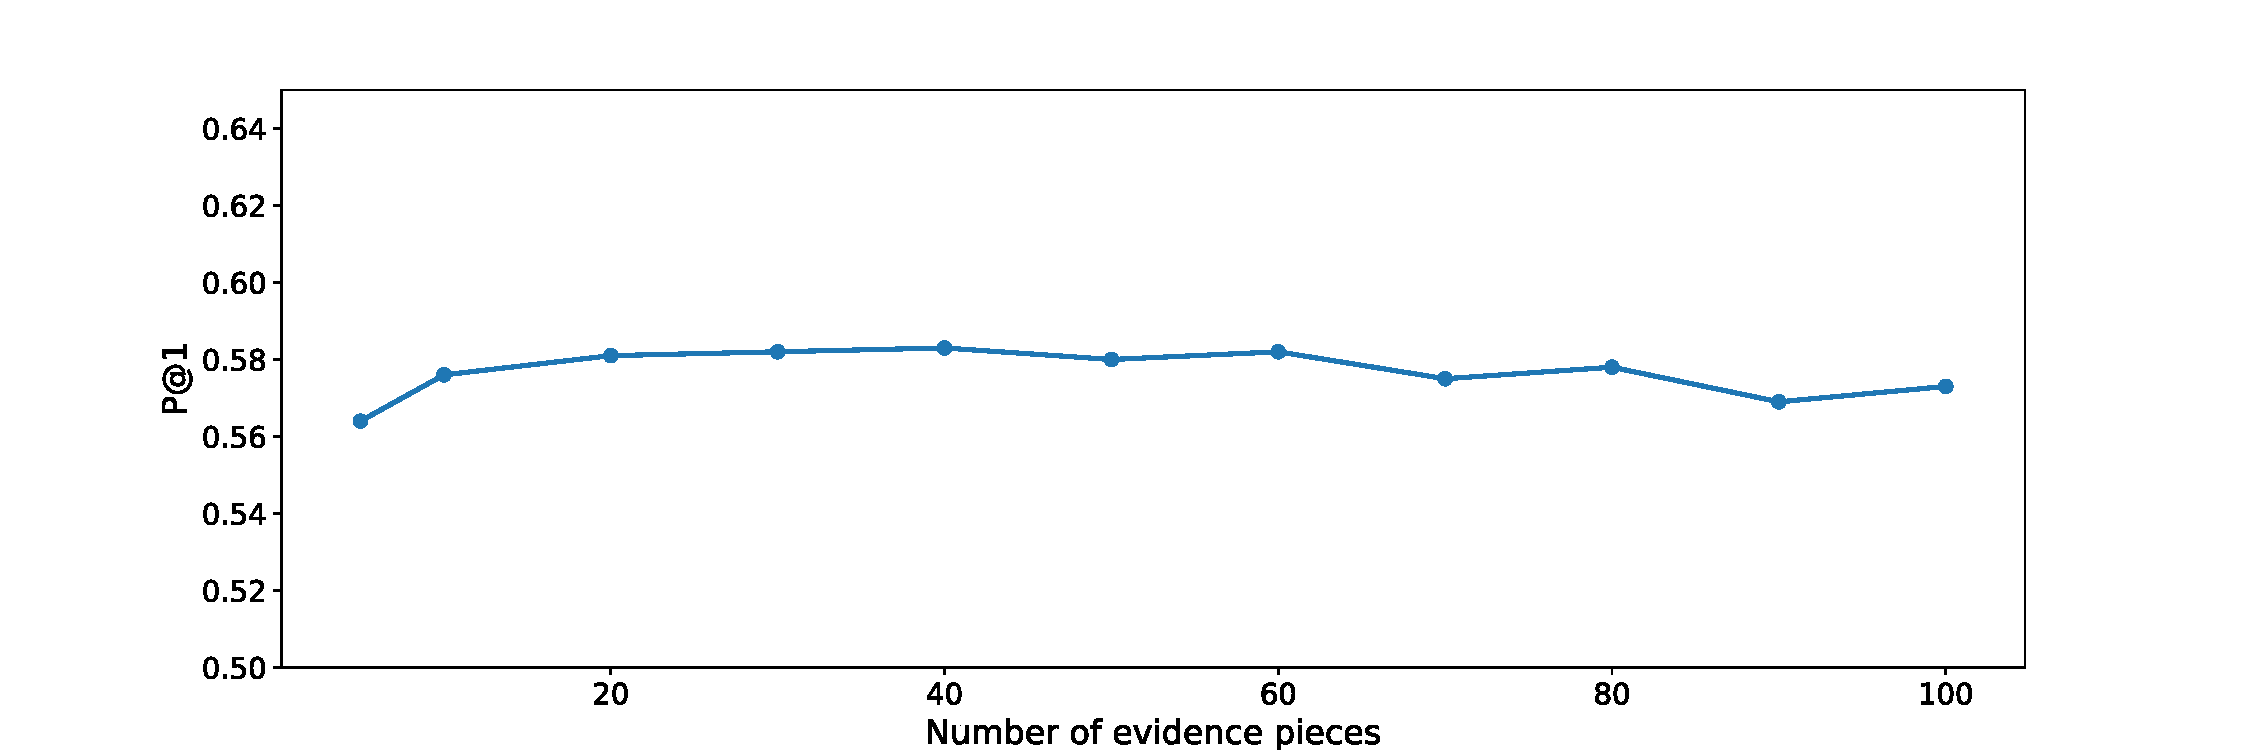
\includegraphics[width=0.8\textwidth]{submissions/Gerhard2024/figures/p_at_1-line_with_evidences.pdf}
    \vspace*{-0.2cm}
    \caption{Performance of \method on the \compmix dev set with different numbers of evidence.}
    \label{fig:res-num-evidences}
    \vspace*{-0.2cm}
\end{figure}



%%% ABLATION
\myparagraph{Ablation study on re-ranking} For more insight on the possible configurations of the RF stage, we conducted an ablation study with different options, including solely relying on the initial BM25 scoring without explicit re-ranking. The results are shown in Table \ref{tab:ablation2}. We observe that the iterative reduction in two steps is slightly better than the single-step variants (going down from top-1000 to top-30 in one RF step). Between the two options of using a GNN or a CE, the differences are negligible. A notable effect is that our RF techniques retain the answer presence at a very high level, only a bit lower than for the initial top-1000. 
The last two rows of Table \ref{tab:ablation2} demonstrate that RF is crucial: without explicit re-ranking, the technique of just picking smaller top-$k$ from the original BM25 model leads to substantial degradation in both answer presence and precision. 


\begin{table} [t] \small
    \centering
    \newcolumntype{G}{>{\columncolor [gray] {0.90}}c}
    \newcolumntype{H}{>{\setbox0=\hbox\bgroup}c<{\egroup}@{}}
    	\begin{tabular}{l G H G G G} 
        \toprule
            & \multicolumn{5}{G}{\textbf{\compmix} (dev set)} \\
        \midrule
            \textbf{RF Method $\downarrow$ / Metric $\rightarrow$} & \textbf{P@1} & \textbf{AP@1000} & \textbf{AP@100}  & \textbf{AP@30} & \textbf{MRR@100} \\ 
        \midrule
            \textbf{GNN: 1000 $\rightarrow$ 100 $\rightarrow$ 30}             &  $\mathbf{0.574}$  & $0.760$ &  $0.738$  &  $0.710$  &  $\mathbf{0.572}$  \\
            \textbf{CE: 1000 $\rightarrow$ 100 $\rightarrow$ 30}          &  $0.573$  & $0.760$  &   $\mathbf{0.740}$ &  $\mathbf{0.721}$   &  $0.553$   \\
        \midrule
            \textbf{GNN: 1000 $\rightarrow$ 30} &  $0.567$  & $?$  &   $n/a$ &  $0.710$   &  $0.567$   \\
         \textbf{CE: 1000 $\rightarrow$ 30} &  $0.570$  & $0.760$  &   $n/a$ &  $0.715$   &  $0.558$   \\
            \midrule
           \textbf{BM25: 100 (w/o GNN or CE)} &  $0.490$ & $0.760$  &  $0.652$  &  $n/a$  &  $0.259$ \\       
            \textbf{BM25: 30 (w/o GNN or CE)} &  $0.468$  & $0.760$  &  $n/a$ &  $0.534$   &  $0.259$   \\
            \bottomrule
    \end{tabular}
    \vspace*{-0.2cm}
    \caption{Ablation study for different RF strategies of \method on the \compmix dev set. The answer presence in the RF input with top-$1000$ evidence pieces is $0.760$.}
    \label{tab:ablation2}
\end{table}



\myparagraph{Quality of SI}
To assess the quality and robustness of the Structured Intents, we
inspected a sample of questions and their SIs.
Table~\ref{tab:question-SI-examples} gives three anecdotic examples.
We show SIs generated by \method, which makes use of the pre-existing collection from the \compmix benchmark for training.
This training data was obtained via different heuristics, 
which can be a limiting factor when user intents become more complex.

Therefore, we also looked at SIs derived via in-context learning (ICL) using \gptfour with $5$ handcrafted examples.
As shown in our earlier work on temporal QA~\cite{Jia-FAITH:WWW2024},
such data can be used for training smaller models (e.g., BART),
which can greatly boost the completeness and overall quality of the generated SIs.

From the sampled set, we observed that the ICL-based SIs are more
complete with all slots filled, whereas the BART-based SIs focused more
on the main slots Answer-type, Entities and Relation.
However, both approaches achieve very high quality in filling the slots,
capturing the user's information need very well.

Interestingly, when questions get complicated, with nested phrases, 
the ICL-based variant succeeds in decomposing the questions, based on only $5$ ICL examples.
For example, for the question {\em ``which German state had the most Corona-related death cases in the first year after the outbreak?''}
the Time slot becomes {\em ``first year after Corona outbreak''},
which can be resolved to identify the temporal scope.
In general, we believe that such question decomposition, beyond simple temporal constraints,
would be an interesting theme for future work.

\begin{table} [t] 
    \centering
    \small
    \newcolumntype{G}{>{\columncolor [gray] {0.90}}c}
    \newcolumntype{H}{>{\setbox0=\hbox\bgroup}c<{\egroup}@{}}
    \resizebox*{\textwidth}{!}{
        \begin{tabular}{p{6cm}|p{6cm}|p{6cm}} 
        \toprule
            \textbf{Question} & \textbf{Current SI by \method} & \textbf{SI via ICL} \\
        \midrule
        \textit{what was disneys first color movie?}
            & Ans-Type: \textit{animated feature film} & Ans-Type: \textit{film, animated film} \\
            & Entities: \textit{disneys} & Entities: \textit{Disney} \\
            & Relation: \textit{was first color movie} & Relation: \textit{first color movie} \\
            &  & Time: \textit{first} \\
        \midrule
        \textit{at the oscars, who won best actor in 2018?}
            & Ans-Type: \textit{human} & Ans-Type: \textit{person, actor} \\
            & Entities: \textit{at the oscars} & Entities: \textit{Oscars, 2018} \\
            & Relation: \textit{who won best actor in 2018} & Relation: \textit{won best actor} \\
            &  & Time: \textit{2018} \\
        \midrule
        \textit{which German state had the most Corona-} & Ans-Type: \textit{state} & Ans-Type: \textit{location, state} \\
        \textit{related death cases in the first year after} & Entities: \textit{Germany, Corona} & Entities: \textit{Germany, Corona-related deaths} \\
        \textit{the outbreak?} & Relation: \textit{which state had the most related} & Relation: \textit{highest count of death cases} \\
        & \textit{death cases in the first year after the out-}  & Location: \textit{Germany} \\
            & \textit{break}  & Time: \textit{first year after Corona outbreak} \\
        \bottomrule
    \end{tabular}
    }
    \vspace*{-0.2cm}
    \caption{Examples for pairs of question and generated SI.}
    \label{tab:question-SI-examples}
\end{table}




%%% REFRAIN FROM ANSWER
\myparagraph{Refraining from answering}
%%% Searched for: "generated_answer I" (with I being the full word, not partial) in the generated answers of LLaMA
%%% yields 245 results out of 2764 questions on CompMix
%%% yields 1270 results out of 3237 questions on TimeQuestions
We can train our model to refrain from answering in scenarios
where the provided evidence does not contain an answer to the question.
Specifically, during training, when the answer is not present in the evidence,
we change the target answer to {\em unknown}. This variant is referred to as \method {\em (faithful)}.

We measure the ratio of questions for which {\em unknown} is provided as answer,
and the P@1 restricted to questions that are answered.
The accuracy of refraining from answering is measured as well,
based on whether the answer is present in the evidence or not.
We conduct this experiment on \compmix and \timequestions,
for which we can compute answer presence exactly.
We also compute results for \llama, which is already instructed 
with the option to answer ``don't know''.
Table~\ref{tab:refrain-from-answer} shows the results.
For \compmix, we observe that \method has high accuracy on refraining when appropriate,
whereas \llama tends to be overconfident with a very small rate of {\em unknowns}, leading to incorrect answers.

\begin{table} [t] \small
    \centering
    \newcolumntype{G}{>{\columncolor [gray] {0.90}}c}
    \newcolumntype{H}{>{\setbox0=\hbox\bgroup}c<{\egroup}@{}}
    	\begin{tabular}{l G G G G c c c c} 
        \toprule
            & \multicolumn{4}{G}{\textbf{\compmix}} & \multicolumn{4}{c}{\textbf{\timequestions}} \\
            \midrule
            \textbf{Metric $\rightarrow$} & \textbf{P@1}  & \textbf{P@1} & \textbf{Refrain} & \textbf{Refrain} & \textbf{P@1}  & \textbf{P@1} & \textbf{Refrain} & \textbf{Refrain} \\ 
            \textbf{Method $\downarrow$} &                 & \textbf{(answered)} & \textbf{rate} & \textbf{accuracy} &                 & \textbf{(answered)} & \textbf{rate} & \textbf{accuracy} \\ 
            \midrule
                \textbf{\llama}             &  $0.431$  &  $0.471$  &  $0.089$  &  $n/a$  &  $0.177$  &  $0.276$  &  $0.392$  &  $n/a$  \\
                \textbf{\method (faithful)}           &  $0.497$  &  $0.713$  &  $0.303$  &  $0.838$ &  $0.597$  &  $0.804$  &  $0.257$  &  $0.864$  \\
            \bottomrule
    \end{tabular}
    \vspace*{-0.2cm}
    \caption{
        Performance of \method with option to refrain from answering (``don't know'').
    }
    \label{tab:refrain-from-answer}
\end{table}

\label{sec:disc}
\section{Insights, Limitations, and Challenges}


\noindent{\bf Benchmark Performance.} Our method, RAG-based \method with an 8B LLaMA model, outperforms much larger LLMs like \gptfour on two of the three benchmarks, with a very large margin for temporal questions. Obviously, pre-trained LLMs have only limited sense of properly positioning ``remembered’’ facts on the timeline even with training data that exceeds ours by several orders of magnitude. This confirms our intuition that LLMs alone are not good at ``recalling’’  higher-arity relations that require combining distant pieces of evidence. This is a sweet spot for RAG. Only for 
the \crag benchmark, \method is substantially inferior to a full-blown LLM. This is likely due to the nature of the questions: not necessarily the complexity of the information needs, but the need for more web sources (beyond what our experiments tap into).

\vspace{0.2cm}
\noindent{\bf Cost/Performance Ratio.} The most important take-away from our experiments is that \method achieves its competitive performance at a much lower cost than the full LLMs. Assuming that the consumed GFlops are proportional to the number of model parameters, \method achieves a cost reduction by a factor of 200x for \gptthree and 2000x for \gptfour. This does not only mean less computation, but also a massively lower electricity bill and climate impact.  

\vspace{0.2cm}
\noindent{\bf Role of Question Understanding.} We did not systematically investigate the influence of the Structured Intent in the \method pipeline. However, the comparison to the big GPT models reflects the role of the SI, as we prompt the GPT models in their natural mode with the original questions. The linearized sequence of available SI slots does not always have major advantages, but there are enough cases where specific facets provide crucial cues. This holds especially for the Entities slot, as this drives the gathering of evidence in the ER stage (cf.~\cite{Christmann-CONVINSE:SIGIR2022}, and for the Time slot, as these cues are often decisive for temporal questions (cf.~\cite{Jia-FAITH:WWW2024}).

\vspace{0.2cm}
\noindent{\bf Role of Re-Ranking.} As our ablation studies show, merely using top-$k$ evidence from an initial BM25-style ranking does not provide good performance. Also, there seems to be sweet spot in the choice of $k$: we need enough evidence for connecting the dots if the question requires multiple pieces of information, or for corroborating candidates if the question finds many useful but noisy pieces. In the experiments, $k=30$ turns out to be good choice; much lower $k$ results in insufficient evidence, and much larger $k$ leads to saturation and ultimately degrading performance. Our argument for iteratively shrinking the candidate set in multiple rounds of re-ranking is substantiated in our experiments, but the gain of doing this, compared to GNN- or CE-based re-ranking from 1000 to 30, is not big. More research is called to better understand the role of ranking in RAG. 

\vspace{0.2cm}
\noindent{\bf Limitations of Evidence Retrieval.}
For ER, we adopted more or less standard techniques. The results showed very good answer presence, in the order of 75\% in the top-100 or even top-30. An important case where this is insufficient are questions that require aggregating information over a large number of evidence pieces. An example is asking for the life-time total of 3-point scores of the basketball player Dirk Nowitzki.
This requires collecting a set of per-season tables with NBA player statistics, but also other web sources with numbers for his career before he joined the NBA (including his youth teams).
Of course, there are sometimes shortcuts like a Wikipedia article or biography mentioning the total number, but this cannot be universally assumed. The bottom line is that ER should be reconsidered as well, striving to improve the recall dimension.

\vspace{0.2cm}
\noindent{\bf Limitations of Answer Generation.}
For AG, we simply rely on a LLM,
using it as an extractor (``reader'') from the given evidence. Despite the wide belief that LLMs can perform deep
reasoning over many pieces of evidence, our experience is that the extraction works only well – robustly and faithfully – for relatively simple questions with a few multi-hop joins or simple aggregation over a few pieces. However, complicated questions such as asking for the top-100 NBA players with the largest number of life-time 3-point scores (again including their pre-NBA careers) are currently out of scope and will likely remain so for quite some time. This offers many opportunities for pushing the envelope further.

\vspace{0.2cm}
\noindent{\bf Trust in Data Sources.}
In our experiments, we considered all heterogeneous sources as trustworthy and unbiased. With focus on Wikidata and Wikipedia, this assumption has been well justified. In the wild, however, input data for RAG-based systems likely exhibit a wide spectrum of quality issues, in terms of stale information, biased positions, or simply false statements. Identifying trustworthy and up-to-date evidence and dealing with conflicting data, has been explored in other contexts (e.g., for KG curation~\cite{Dong-Trust:PVLDB2015}), but remains a major challenge for RAG-based QA.


\vspace{0.2cm}
\noindent{\bf Open Challenges and Future Work.} The best-performing methods in our experiment, mostly \method, reach P@1 values of 56\% for \compmix and 75\% for \timequestions. 
For the latter, the answer presence in the top-100 is only slightly higher; so the AG stage hardly misses anything.
However, for \compmix, the answer presence is 75\% -- much higher than what our system can actually answer. Obviously, closing this gap is a major direction to pursue, with focus on the RF and AG stages. However, missing one fourth of the answers completely in the top-100 pool, is a big problem as well. This requires improving recall at the ER stage, possibly with better guidance by the QU, which in turn needs more sources beyond the scope of our experiments (currently limited to Wikidata and Wikipedia). 

In general, we need to think beyond this kind of ``benchmark mindset’’. Even if we reached 80\% or 90\% precision and recall, we would still have a substantial fraction of questions that are answered incorrectly
or not at all. 
The remaining errors may not be a problem for chatbots, but they would be a showstopper for the deployment of mission-critical applications in business or science. We believe that this big gap is a shortcoming of {\em all methods}, not an issue that comes from the data alone. For trivia-style QA, as looked at in this paper, a smart human in ``open book’’ mode and no time limitation should be able to properly answer practically all questions, just by reading pieces of web contents and putting things together. Neither LLMs nor state-of-the-art RAG are the final solution; substantial research and creative ideas are needed to further advance QA.


\clearpage
\newpage

\newcommand{\bibauthors}[1]{{#1}}
\newcommand{\bibtitle}[1]{\emph{#1}}
\newcommand{\bibconf}[1]{{#1}}

\begin{thebibliography}{10}

\bibitem{Bajaj:arxiv2018}
\bibauthors{Payal Bajaj, Daniel Campos, Nick Craswell, Li Deng, Jianfeng Gao, Xiaodong Liu, Rangan Majumder, Andrew McNamara, Bhaskar Mitra, Tri Nguyen, Mir Rosenberg, Xia Song, Alina Stoica, Saurabh Tiwary, Tong Wang.}
\bibtitle{MS MARCO: A Human Generated MAchine Reading COmprehension Dataset.}
In \bibconf{arXiv 2018}.

\bibitem{DBLP:conf/acl/ChenFWB17}
\bibauthors{Danqi Chen, Adam Fisch, Jason Weston and Antoine Bordes.}
\bibtitle{Reading Wikipedia to Answer Open-Domain Questions.}
In \bibconf{ACL 2017}.

\bibitem{Christmann-CONVINSE:SIGIR2022}
\bibauthors{Philipp Christmann, Rishiraj Saha Roy, Gerhard Weikum.}
\bibtitle{Conversational Question Answering on Heterogeneous Sources.}
In \bibconf{SIGIR 2022}.

\bibitem{Christmann-CLOCQ:WSDM2022}
\bibauthors{Philipp Christmann, Rishiraj Saha Roy, Gerhard Weikum.}
\bibtitle{Beyond NED: Fast and Effective Search Space Reduction for Complex Question Answering over Knowledge Bases.}
In \bibconf{WSDM 2022}.

\bibitem{Christmann-Explaignn:SIGIR2023}
\bibauthors{Philipp Christmann, Rishiraj Saha Roy, Gerhard Weikum.}
\bibtitle{Explainable Conversational Question Answering over Heterogeneous Sources via Iterative Graph Neural Networks.}
In \bibconf{SIGIR 2023}.

\bibitem{Christmann-CompMix:WWW2024}
\bibauthors{Philipp Christmann, Rishiraj Saha Roy, Gerhard Weikum.}
\bibtitle{CompMix: A Benchmark for Heterogeneous Question Answering.}
In \bibconf{WWW 2024}.

\bibitem{Dejean:arxiv2024}
\bibauthors{Herve Dejean, Stephane Clinchant, Thibault Formal.}
\bibtitle{A Thorough Comparison of Cross-Encoders and LLMs for Reranking SPLADE.}
In \bibconf{arXiv 2024}.

\bibitem{Dhingra-time-aware-LLM:TACL2022}
\bibauthors{Bhuwan Dhingra, Jeremy R Cole, Julian Martin Eisenschlos, Daniel Gillick, Jacob Eisenstein, and William W Cohen.}
\bibtitle{Time-Aware Language Models as Temporal Knowledge Bases.}
In \bibconf{TACL 2022}.

\bibitem{Dong-Trust:PVLDB2015}
\bibauthors{Xin Luna Dong, Evgeniy Gabrilovich, Kevin Murphy, Van Dang, Wilko Horn, Camillo Lugaresi, Shaohua Sun, Wei Zhang.}
\bibtitle{Knowledge-Based Trust: Estimating the Trustworthiness of Web Sources.}
In \bibconf{PVLDB 2015}.

\bibitem{DBLP:journals/arXiv/abs-2312-10997}
\bibauthors{Yunfan Gao, Yun Xiong, Xinyu Gao, Kangxiang Jia, Jinliu Pan, Yuxi Bi, Yi Dai, Jiawei Sun, Qianyu Guo, Meng Wang, Haofen Wang.}
\bibtitle{Retrieval-Augmented Generation for Large Language Models: A Survey.}
In \bibconf{arXiv 2023}.

\bibitem{Gao-citations:emnlp2023}
\bibauthors{Tianyu Gao, Howard Yen, Jiatong Yu, Danqi Chen.}
\bibtitle{Enabling Large Language Models to Generate Text with Citations.}
In \bibconf{EMNLP 2023}.

\bibitem{Guu-REALM:ICML2020}
\bibauthors{Kelvin Guu, Kenton Lee, Zora Tung, Panupong Pasupat, Ming-Wei Chang.}
\bibtitle{Retrieval Augmented Language Model Pre-Training.}
In \bibconf{ICML 2020}.

\bibitem{DBLP:conf/eacl/IzacardG21}
\bibauthors{Gautier Izacard, Edouard Grave.}
\bibtitle{Leveraging Passage Retrieval with Generative Models for Open Domain Question Answering.}
In \bibconf{EACL 2021}.

\bibitem{Jia-TimeQuestions}
\bibauthors{Zhen Jia, Soumajit Pramanik, Rishiraj Saha Roy, and Gerhard Weikum.}
\bibtitle{Complex Temporal Question Answering on Knowledge Graphs.}
In \bibconf{CIKM 2021}.

\bibitem{Jia-FAITH:WWW2024}
\bibauthors{Zhen Jia, Philipp Christmann, Gerhard Weikum.}
\bibtitle{Faithful Temporal Question Answering over Heterogeneous Sources.}
In \bibconf{WWW 2024}.

\bibitem{DBLP:journals/arXiv/abs-2305-06984}
\bibauthors{Ehsan Kamalloo, Nouha Dziri, Charles L. A. Clarke, Davood Rafiei.}
\bibtitle{Evaluating Open-Domain Question Answering in the Era of Large Language Models.}
In \bibconf{arXiv 2023}.

\bibitem{Kandpal:ICML2023}
\bibauthors{Nikhil Kandpal, Haikang Deng, Adam Roberts, Eric Wallace, Colin Raffel.}
\bibtitle{Large Language Models Struggle to Learn Long-Tail Knowledge.}
In \bibconf{ICML 2023}.

\bibitem{DBLP:conf/emnlp/KarpukhinOMLWEC20}
\bibauthors{Vladimir Karpukhin, Barlas Oguz, Sewon Min, Patrick S. H. Lewis, Ledell Wu, Sergey Edunov, Danqi Chen, Wen-tau Yih.}
\bibtitle{Dense Passage Retrieval for Open-Domain Question Answering.}
In \bibconf{EMNLP 2020}.

\bibitem{Lee-MATTER:ACL2024}
\bibauthors{Dongkyu Lee, Chandana Satya Prakash, Jack FitzGerald, Jens Lehmann.}
\bibtitle{MATTER: Memory-Augmented Transformer Using Heterogeneous Knowledge Sources.}
In \bibconf{ACL 2024}.

\bibitem{DBLP:conf/acl/LewisLGGMLSZ20}
\bibauthors{Mike Lewis, Yinhan Liu, Naman Goyal, Marjan Ghazvininejad, Abdelrahman Mohamed, Omer Levy, Veselin Stoyanov, Luke Zettlemoyer.}
\bibtitle{BART: Denoising Sequence-to-Sequence Pre-training for Natural Language Generation, Translation, and Comprehension.}
In \bibconf{ACL 2020}.

\bibitem{DBLP:conf/nips/LewisPPPKGKLYR020}
\bibauthors{Patrick S. H. Lewis, Ethan Perez, Aleksandra Piktus, Fabio Petroni, Vladimir Karpukhin, Naman Goyal, Heinrich Küttler, Mike Lewis, Wen-tau Yih, Tim Rocktäschel, Sebastian Riedel, Douwe Kiela.}
\bibtitle{Retrieval-Augmented Generation for Knowledge-Intensive NLP Tasks.}
In \bibconf{NeurIPS 2020}.

\bibitem{Lin:MC2021}
\bibauthors{Jimmy Lin, Rodrigo Frassetto Nogueira, Andrew Yates.}
\bibtitle{Pretrained Transformers for Text Ranking: BERT and Beyond.}
In \bibconf{Morgan \& Claypool Publishers 2021}.

\bibitem{Liu-SUQL:NAACL2024}
\bibauthors{Shicheng Liu, Jialiang Xu, Wesley Tjangnaka, Sina J. Semnani, Chen Jie Yu, Monica Lam.}
\bibtitle{SUQL: Conversational Search over Structured and Unstructured Data with Large Language Models.}
In \bibconf{NAACL-HLT 2024}.

\bibitem{Mavi:FnT2024}
\bibauthors{Vaibhav Mavi, Anubhav Jangra, Adam Jatowt.}
\bibtitle{Multi-hop Question Answering.}
In \bibconf{Foundations and Trends in Information Retrieval 2024}.

\bibitem{Minaee-LLM-survey}
\bibauthors{Shervin Minaee, Tomas Mikolov, Narjes Nikzad, Meysam Chenaghlu, Richard}
\bibtitle{Socher, Xavier Amatriain, and Jianfeng Gao.}
Large Language Models: A Survey.
In \bibconf{arXiv 2024}.

\bibitem{Nogueira:arxiv2019}
\bibauthors{Rodrigo Frassetto Nogueira, Kyunghyun Cho.}
\bibtitle{Passage Re-ranking with BERT.}
In \bibconf{arXiv 2019}.

\bibitem{Oguz-UniK-QA:NAACL2022}
\bibauthors{Barlas Oguz, Xilun Chen, Vladimir Karpukhin, Stan Peshterliev, Dmytro Okhonko, Michael Sejr Schlichtkrull, Sonal Gupta, Yashar Mehdad, Scott Yih.}
\bibtitle{UniK-QA: Unified Representations of Structured and Unstructured Knowledge for Open-Domain Question Answering.}
In \bibconf{NAACL-HLT 2022}.

\bibitem{RogersGA:CS2023}
\bibauthors{Anna Rogers, Matt Gardner, Isabelle Augenstein.}
\bibtitle{QA Dataset Explosion: A Taxonomy of NLP Resources for Question Answering and Reading Comprehension.}
In \bibconf{ACM Computing Surveys 2023}.

\bibitem{RoyAnand:MC2021}
\bibauthors{Rishiraj Saha Roy, Avishek Anand.}
\bibtitle{Question Answering for the Curated Web: Tasks and Methods in QA over Knowledge Bases and Text Collections.}
In \bibconf{Synthesis Lectures on Information Concepts, Retrieval, and Services, Morgan \& Claypool Publishers 2021}.

\bibitem{Pramanik-Uniqorn:JWS2024}
\bibauthors{Soumajit Pramanik, Jesujoba Alabi, Rishiraj Saha Roy, Gerhard Weikum.}
\bibtitle{UNIQORN: Unified Question Answering over RDF Knowledge Graphs and Natural Language Text.}
In \bibconf{Journal of Web Semantics 2024}.

\bibitem{Sun-PullNet:EMNLP2019}
\bibauthors{Haitian Sun, Tania Bedrax-Weiss, William W. Cohen.}
\bibtitle{PullNet: Open Domain Question Answering with Iterative Retrieval on Knowledge Bases and Text.}
In \bibconf{EMNLP/IJCNLP 2019}.

\bibitem{Sun:NAACL2024}
\bibauthors{Kai Sun, Yifan Ethan Xu, Hanwen Zha, Yue Liu, Xin Luna Dong.}
\bibtitle{Head-to-Tail: How Knowledgeable are Large Language Models (LLMs)? A.K.A. Will LLMs Replace Knowledge Graphs?}
In \bibconf{NAACL-HLT 2024}.

\bibitem{Touvron-LLaMA}
\bibauthors{Hugo Touvron, Thibaut Lavril, Gautier Izacard, Xavier Martinet, Marie-Anne Lachaux, Timothée Lacroix, Baptiste Rozière, Naman Goyal, Eric Hambro, Faisal Azhar, Aurelien Rodriguez, Armand Joulin, Edouard Grave, Guillaume Lample.}
\bibtitle{Llama: Open and efficient foundation language models.}
In \bibconf{arXiv 2023}.

\bibitem{Wu-STARK:arxiv2024}
\bibauthors{Shirley Wu, Shiyu Zhao, Michihiro Yasunaga, Kexin Huang, Kaidi Cao, Qian Huang, Vassilis N. Ioannidis, Karthik Subbian, James Zou, Jure Leskovec.}
\bibtitle{STaRK: Benchmarking LLM Retrieval on Textual and Relational Knowledge Bases.}
In \bibconf{arXiv 2024}.

\bibitem{Wu:IEEE2021}
\bibauthors{Zonghan Wu, Shirui Pan, Fengwen Chen, Guodong Long, Chengqi Zhang, Philip S. Yu.}
\bibtitle{A Comprehensive Survey on Graph Neural Networks.}
In \bibconf{IEEE Transactions on Neural Networks and Learning Systems 2021}.

\bibitem{Yang-CRAG}
\bibauthors{Xiao Yang, Kai Sun, Hao Xin, Yushi Sun, Nikita Bhalla, Xiangsen Chen, Sajal Choudhary, Rongze D. Gui, Ziran W. Jiang, Ziyu Jiang, Lingkun Kong, Brian Moran, Jiaqi Wang, Yifan Ethan Xu, An Yan, Chenyu Yang, Eting Yuan, Hanwen Zha, Nan Tang, Lei Chen, Nicolas Scheffer, Yue Liu, Nirav Shah, Rakesh Wanga, Anuj Kumar, Wen-tau Yih, Xin Luna Dong.}
\bibtitle{CRAG -- Comprehensive RAG Benchmark.}
In \bibconf{arXiv 2024}.

\bibitem{Yasunaga:NAACL2021}
\bibauthors{Michihiro Yasunaga, Hongyu Ren, Antoine Bosselut, Percy Liang, Jure Leskovec.}
\bibtitle{QA-GNN: Reasoning with Language Models and Knowledge Graphs for Question Answering.}
In \bibconf{NAACL-HLT 2021}.

\bibitem{Zhang-Spaghetti:ACL2024}
\bibauthors{Heidi C. Zhang, Sina J. Semnani, Farhad Ghassemi, Jialiang Xu, Shicheng Liu, Monica S. Lam.}
\bibtitle{SPAGHETTI: Open-Domain Question Answering from Heterogeneous Data Sources with Retrieval and Semantic Parsing.}
In \bibconf{ACL 2024}.

\bibitem{Zhang:NAACL2024}
\bibauthors{Jiahao Zhang, Haiyang Zhang, Dongmei Zhang, Yong Liu, Shen Huang.}
\bibtitle{End-to-End Beam Retrieval for Multi-Hop Question Answering.}
In \bibconf{NAACL-HLT 2024}.

\bibitem{Zhao-LLMsurvey}
\bibauthors{Wayne Xin Zhao, Kun Zhou, Junyi Li, Tianyi Tang, Xiaolei Wang, Yupeng Hou, Yingqian Min, Beichen Zhang, Junjie Zhang, Zican Dong, Yifan Du, Chen Yang, Yushuo Chen, Zhipeng Chen, Jinhao Jiang, Ruiyang Ren, Yifan Li, Xinyu Tang, Zikang Liu, Peiyu Liu, Jian-Yun Nie, Ji-Rong Wen.}
\bibtitle{A Survey of Large Language Models.}
In \bibconf{arXiv 2023}.

\bibitem{Zhao:arxiv2024}
\bibauthors{Penghao Zhao, Hailin Zhang, Qinhan Yu, Zhengren Wang, Yunteng Geng, Fangcheng Fu, Ling Yang, Wentao Zhang, Bin Cui.}
\bibtitle{Retrieval-Augmented Generation for AI-Generated Content: A Survey.}
In \bibconf{arXiv 2024}.

\bibitem{Zhu-ODQA-survey:arxiv2021}
\bibauthors{Fengbin Zhu, Wenqiang Lei, Chao Wang, Jianming Zheng, Soujanya Poria, Tat-Seng Chua.}
\bibtitle{Retrieving and Reading: A Comprehensive Survey on Open-domain Question Answering.}
In \bibconf{arXiv 2021}.

\end{thebibliography}


\end{document}

\end{article}
\begin{article}
{User Modeling in the Era of Large Language Models: Current Research and Future Directions}
{Zhaoxuan Tan, Meng Jiang}
\setcounter{section}{0}
\documentclass{article}

\usepackage{deauthor}

\usepackage{latexsym}
\usepackage{graphicx}
\graphicspath{{./images/}}
\usepackage{booktabs} % for formal tables
\usepackage{color}  % for coloring text
\usepackage{amsmath}  % for aligning equations
\usepackage{subcaption}
\usepackage{caption}
\usepackage{tikz}
\usepackage{colortbl} % for color in tables
\usepackage{framed}
\usepackage{multirow}
\usepackage{multicol}
\usepackage{hyperref}
\usepackage{url}
\usepackage{balance}
\usepackage{verbatim}
\usepackage{cancel}
\usepackage{xspace} % for correcting space after macro commands
\usepackage{algorithm2e}
\usepackage{bbold} % for writing mathbb{1}
\usepackage{balance}
\usepackage{stmaryrd}
\usepackage{enumitem}
\usepackage{array} % package for hiding a column
\usepackage{bold-extra} % to enable textbf with textsc

% used for making text readable in document and .tex
% \setlength{\parindent}{0pt}

\newcommand{\struct}[1]{\texttt{\small #1}}
\newcommand{\utterance}[1]{\textit{#1}}
\newcommand{\phrase}[1]{\textit{``#1''}}

% \newcommand {\g}[1]{\textcolor[gray]{0.6}{#1}}

\newcommand{\drop}{\dag\xspace}

\newenvironment{Snugshade}[1][236,236,236]{
    \setlength{\itemsep}{0pt}
     \setlength{\parsep}{0pt}
     \setlength{\topsep}{0pt}
     \setlength{\partopsep}{0pt}
     \setlength{\leftmargin}{1.5em}
     \setlength{\labelwidth}{0em}
     \setlength{\labelsep}{0em} 
    \setlength{\parskip}{0pt}
    \definecolor{shadecolor}{RGB}{#1}
    \begin{snugshade}
}{
    \end{snugshade}
}


\newcommand{\method}{\textsc{Quasar}\xspace}
\newcommand{\benchmark}{\textsc{PerQA}\xspace}
\newcommand{\itemslist}[1]{$\langle$\struct{#1}$\rangle$}


\newcommand{\convinse}{\textsc{Convinse}\xspace}
\newcommand{\explaignn}{\textsc{Explaignn}\xspace}
\newcommand{\clocq}{\textsc{Clocq}\xspace}
\newcommand{\unikqa}{\textsc{UniK-Qa}\xspace}
\newcommand{\gptthree}{\textsc{Gpt-3}\xspace}
\newcommand{\gptfour}{\textsc{Gpt-4}\xspace}
\newcommand{\llama}{\textsc{Llama3}\xspace}
\newcommand{\spaghetti}{\textsc{Spaghetti}\xspace}


\newcommand{\compmix}{\textsc{CompMix}\xspace}
\newcommand{\timequestions}{\textsc{TimeQuestions}\xspace}
\newcommand{\crag}{\textsc{Crag}\xspace}


\newcommand{\squishlist}{
    \begin{list}{$\bullet$}{
        \setlength{\itemsep}{0pt}
	\setlength{\parsep}{3pt}
	\setlength{\topsep}{3pt}
	\setlength{\partopsep}{0pt}
	\setlength{\leftmargin}{1.5em}
	\setlength{\labelwidth}{1em}
	\setlength{\labelsep}{0.5em}
    }
}

\newcommand{\squishend}{
    \end{list}
}

\newcommand{\myparagraph}[1]{\vspace*{0.2cm}\noindent \textbf{#1}.}
\newcommand{\myparagraphnospace}[1]{\noindent \textbf{#1}.}

% \newcommand{\GW}[1]{\emph{{\color{blue} GW:#1}}}
% \newcommand{\PC}[1]{\emph{{\color{orange} PC: #1}}}
% \newcommand{\tocite}{{{\color{red} [CITE]}}}


\begin{document}

\title{RAG-based Question Answering \\ over Heterogeneous Data and Text}

\author{
Philipp Christmann,
Gerhard Weikum\\\\
Max Planck Institute for Informatics\\
Saarland Informatics Campus, Germany\\
\texttt{\{pchristm, weikum\}@mpi-inf.mpg.de}}

\maketitle

\section*{Abstract}
This article presents the \method system for question answering over unstructured text, structured tables, and knowledge graphs, with unified treatment of all sources.
The system adopts a RAG-based architecture, with a pipeline of evidence retrieval followed by answer generation, with the latter powered by a 
moderate-sized
language model.
Additionally and uniquely, \method
has components for question understanding, to derive crisper input for evidence retrieval, and for re-ranking and filtering the retrieved evidence before feeding the most informative pieces into the answer generation.
Experiments with three different benchmarks demonstrate the high answering quality of our approach, being on par with or better than large GPT models, while keeping the computational cost and energy consumption orders of magnitude lower.

\label{sec:intro}
\section{Introduction}

\noindent\textbf{Motivation and Problem.} The task of question answering, QA for short, arises in many flavors: factual vs. opinions, simple lookups vs. multi-hop inference, single answer vs. list of entities, 
direct answers vs. long-form, one-shot questions vs. conversations, and other varieties 
(see, e.g., surveys~\cite{RogersGA:CS2023,RoyAnand:MC2021}).
The state-of-the-art for this entire spectrum has been greatly advanced in the past decade. Most notably, incorporating deep learning into retriever-reader architectures (e.g.,~\cite{DBLP:conf/acl/ChenFWB17,DBLP:conf/eacl/IzacardG21,DBLP:conf/emnlp/KarpukhinOMLWEC20}) has boosted answering quality, and most recently, large language models (LLM)~\cite{Minaee-LLM-survey,Zhao-LLMsurvey} have pushed the envelope even further (e.g.,~\cite{DBLP:journals/arXiv/abs-2305-06984}).

% strengths and limitations of LLM for QA
Today’s LLMs alone are capable of accurately answering many \textit{factoid} questions, simply from their pre-trained parametric memory which latently encodes huge text corpora and other online contents.
However, this critically depends on the frequency of evidence in the underlying contents and the complexity of the information need. 
For example, 
asking for the {\em MVP of the 2024 NBA season} would easily return the correct answer Nikola Jokic, 
but asking for the {\em highest-scoring German NBA player} or the {\em MVP of the 2024 German basketball league} pose a big challenge.
The reason is that LLMs alone do not easily recall information about not so popular or even long-tail entities~\cite{Kandpal:ICML2023,Sun:NAACL2024},
and that they are mainly geared for direct look-ups as opposed to connecting multiple pieces of evidence~\cite{Mavi:FnT2024,Zhang:NAACL2024}.

% introduce RAG and discuss need for heterogeneous sources
\cite{DBLP:journals/arXiv/abs-2312-10997,Guu-REALM:ICML2020,DBLP:conf/nips/LewisPPPKGKLYR020,Zhao:arxiv2024}
known as RAG, address these bottlenecks. In addition to cleverly crafted prompts and few-shot examples, the LLM is provided with the top-ranked results of an explicit retrieval step, like web search or knowledge graph (KG) lookups. The former is often necessary for freshness of answers, and the latter may help with long-tail entities and also mitigate the notorious risk of hallucinations. Still, this generation’s RAG architectures are limited in how broad and how deep they tap into external sources. Popular AI assistants like Gemini or ChatGPT seem to primarily retrieve from the text of web pages (incl. Wikipedia articles), and academic research has additionally pursued knowledge augmentation by enhancing prompts with facts from large KGs (e.g., Wikidata).

An additional content modality that is still underexplored are {\em online tables}: a wide range of tabular data including HTML tables in web pages, spreadsheets and statistics, all the way to CSV and JSON datasets that are abundant on the Internet. There is prior work on joint support for text and KGs and for text and tables, but very little on all of these together -- some notable exceptions being~\cite{Christmann-CONVINSE:SIGIR2022,Christmann-Explaignn:SIGIR2023,Oguz-UniK-QA:NAACL2022,Zhang-Spaghetti:ACL2024}.


\noindent\textbf{Examples.} All three heterogeneous types of sources are crucial not only for answering different questions from different kinds of evidence, but also for combining multiple pieces of evidence of different modalities to infer correct and complete answers.
To 
illustrate
the need for tapping all sources, consider the following questions:

% \vspace*{0.2cm}
\begin{quote}
$Q1$: \utterance{Which Chinese basketballers have played in the NBA?}\\
 \indent $Q2$: \utterance{Who was the first Chinese NBA player?}\\
  \indent $Q3$: \utterance{Which Chinese NBA player has the most matches?}
\end{quote}
% \vspace*{0.2cm}

Q1 can be cast into querying a KG, but the list there is not necessarily complete and up-to-date, so additional evidence from text or tables would be desired. 
Q2 needs information about who played in which seasons, found only in web pages or sports-statistics tables. 
Finally, Q3 may be lucky in finding prominent textual evidence (e.g., in biographies, Wikipedia etc.), but this often faces divergent statements, and resolving contradictions needs to dive into more evidence. Besides, when textual evidence is rare and hard to find or not trustworthy enough, then information from multiple tables and text snippets may have to be aggregated (e.g., totals of per-season counts).
Some of this may perhaps become feasible for an industrial LLM’s RAG capabilities in the near future, but there are always harder scenarios by moving from Chinese NBA players deeper into the long tail, such as asking for {\em Lithuanian players in the German handball league}.

\vspace*{0.2cm}
\noindent\textbf{Approach and Contribution.} This paper presents a simple but powerful and versatile RAG system with unified access to text, KG and tables. We call our method {\em \method} 
(for Question Answering over Heterogeneous Sources with Augmented Retrieval).
Its architecture is relatively straightforward: all heterogeneous content is verbalized and indexed for retrieval; a retriever finds top-ranked results for the given question (from different source types), and these are fed into the LLM for answer generation. This is the unsurprising bird-eye’s view. Specific details that are key factors for the strong performance of \method are: 

\squishlist
\item[i)] automatically casting user questions into a structured representation of the information need, which is then used to guide 
\item[ii)] judicious ranking of search results, with multiple rounds of re-ranking and pruning, followed by
\item[iii)]	extracting faithful answers from an LLM in RAG mode, with answers grounded in tangible evidence.
\squishend


\vspace{0.2cm}
\noindent The paper presents experiments with three different benchmarks, covering various flavors of questions.
We focus on one-shot questions; conversational QA is out of scope here, but \method itself is well applicable to this case, too.
Our experiments demonstrate that our methods are competitive, on par with big GPT models and often better,
while being several orders of magnitude lower in computational and energy cost.
The experimental findings also highlight that question understanding, with structured representation of user intents, and iterative re-ranking of evidence are crucial for good performance.

Overall, our contribution lies in proposing a unified system architecture for RAG-based question answering over a suite of different data sources, with strong points regarding both effectiveness (i.e., answer quality)
and efficiency (i.e., computational cost).


\label{sec:background}
\section{Related Work}

The RAG paradigm came up as a principled way of enhancing LLM factuality incl. provenance and mitigating the risk of hallucination~\cite{Guu-REALM:ICML2020, DBLP:conf/nips/LewisPPPKGKLYR020}.
It is highly related to the earlier
retriever-reader architectures for QA~\cite{DBLP:conf/acl/ChenFWB17,DBLP:conf/emnlp/KarpukhinOMLWEC20}, especially when the reader uses the fusion-in-decoder method~\cite{DBLP:conf/eacl/IzacardG21,Oguz-UniK-QA:NAACL2022}.
Since its invention, RAG methodology has been greatly advanced, introducing a wide suite of extensions, such as batched inputs, interleaving retrieval and generation steps, and more (see the recent surveys~\cite{DBLP:journals/arXiv/abs-2312-10997,Zhao:arxiv2024}).

On question answering (QA), there is a vast amount of literature including a wealth of differently flavored benchmarks (see, e.g.,~\cite{RogersGA:CS2023}).
The case of interest here is QA over heterogeneous sources, tapping into both unstructured content and structured data. 
A variety of works has pursued this theme by combining knowledge graphs with text sources, using graph-based methods, neural learning and  language models (e.g.,~\cite{Pramanik-Uniqorn:JWS2024,Sun-PullNet:EMNLP2019,Yasunaga:NAACL2021}).

Most relevant for this article is the research on jointly leveraging all different sources: text, KGs, and tables (incl. CSV and JSON files). This includes  
the \unikqa system~\cite{Oguz-UniK-QA:NAACL2022},
the \spaghetti/SUQL project~\cite{Liu-SUQL:NAACL2024,Zhang-Spaghetti:ACL2024},
the \textsc{Matter} method~\cite{Lee-MATTER:ACL2024},
the STaRK benchmarking~\cite{Wu-STARK:arxiv2024},
and our own prior work
~\cite{Christmann-CONVINSE:SIGIR2022,Christmann-Explaignn:SIGIR2023} (without claiming exhaustiveness).
Out of these, we include \unikqa, \spaghetti and our own systems \convinse and \explaignn as baselines in the experimental evaluation.
Their architectures are similar to ours, but \unikqa and \spaghetti do not have our distinctive elements of
question understanding and iterative re-ranking (originally introduced in \explaignn~\cite{Christmann-Explaignn:SIGIR2023}).

\label{sec:method}
\section{Methodology}

\begin{figure}[tb]
  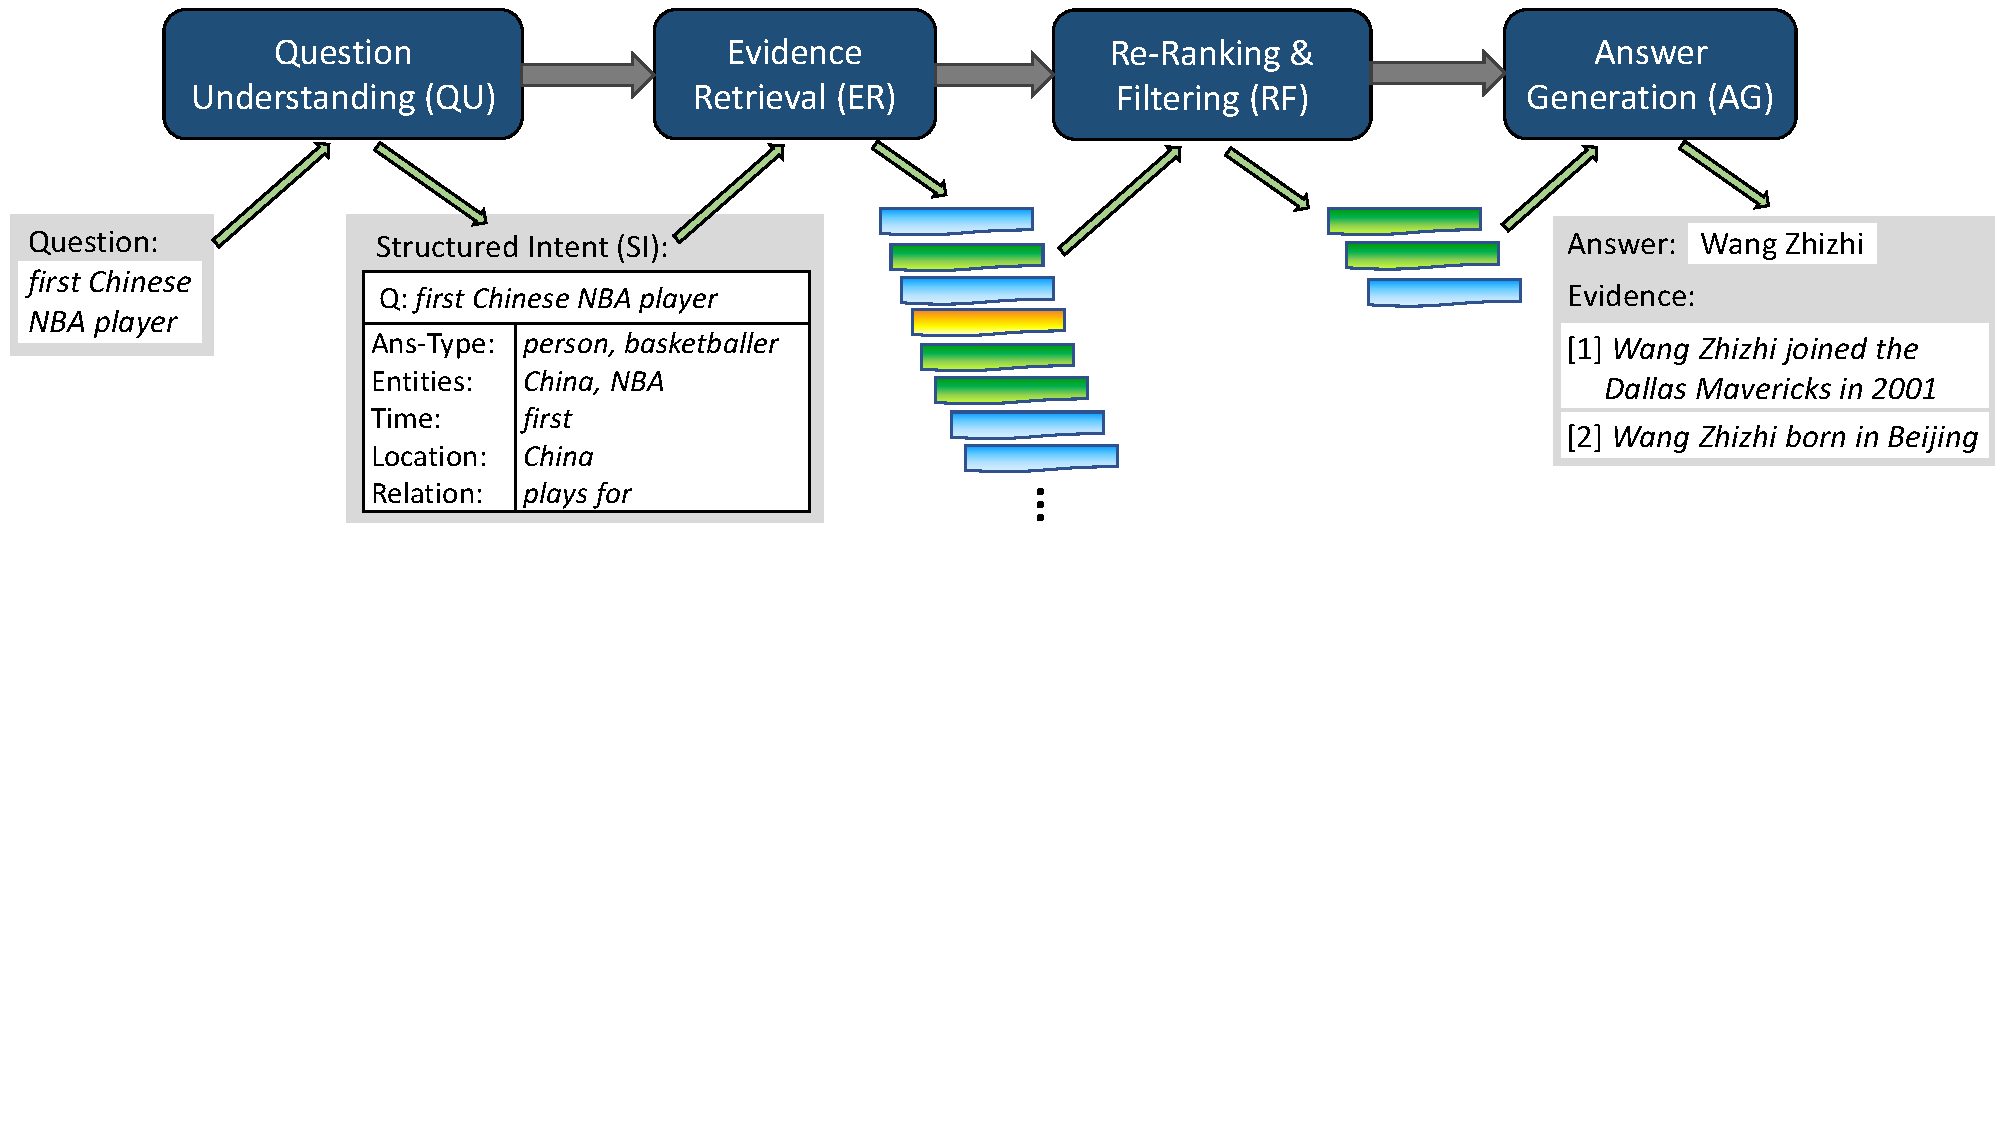
\includegraphics[width=\textwidth]{submissions/Gerhard2024/figures/compass-overview.pdf}
  \caption{Overview of the \method system.}
  \label{fig:compass-overview}
\end{figure}

% start with system overview
The \method system is a pipeline of four major stages, as illustrated in Figure \ref{fig:compass-overview}.
First, the input question is analyzed and decomposed, in order to compute a {\em structured intent (SI)} representation that will pass on to the subsequent steps, along with the original question. Second, the SI is utilized to retrieve pieces of evidence from different sources: text, KG and tables. 
Third, this pool of potentially useful evidence is filtered down, with iterative re-ranking, to arrive at a tractably small set of most promising evidence.
The final stage generates the answer from this evidence,
passing back the answer as well as evidence snippets for user-comprehensible explanation.

The second and fourth stage, Evidence Retrieval (ER) and Answer Generation (AG), are fairly standard. Such a two-phase architecture was called a retriever-reader architecture~\cite{Zhu-ODQA-survey:arxiv2021}. With a modern LLM replacing the earlier kinds of neural readers, this is the core of every RAG system~\cite{DBLP:journals/arXiv/abs-2312-10997}.

Stages 1 and 3 are unique elements of our architecture, judiciously introduced to improve both effectiveness (i.e., answer quality) and efficiency (i.e., computational cost).
Question Understanding (QU) provides the ER component with crisper and semantically refined input, and
the Re-Ranking \& Filtering (RF) stage is beneficial for
distilling the best evidence from the large pool of retrieved pieces.
The following subsections elaborate on the four stages of the pipeline, emphasizing the \method-specific steps QU and RF.



\subsection{Question Understanding (QU)}

% one par introducing the SI
To prepare the retrieval from different kinds of sources, including a KG, ad-hoc tables and text documents, it is useful to analyze and decompose the user question.
In this work, we aim to cast a question into a 
{\em structured intent (SI)} representation: essentially
a frame with faceted cues as slots, or equivalently, a concise set of key-value pairs. 
Figure \ref{fig:compass-overview} gives an idealized example for the question about the first Chinese NBA player. The facets or keys of potential interest here 
are:
\squishlist
\item {\em Ans-Type:} the expected answer type (or types when considering
different levels of semantic refinement), 
\item {\em Entities:} the salient entities in the question, and 
\item {\em Relation:} phrases that indicate which relation (between Q and A entities) the user is interested in. 
\squishend
\noindent In addition, as questions can have temporal or spatial aspects, the SI also foresees slots for:
\squishlist
\item {\em Time:} cues about answer-relevant time points or spans, including relative cues (e.g., ``before Covid'') and ordinal cues (e.g., ``first''), and
\item {\em Location:} cues about answer-relevant geo-locations.
\squishend

% discuss the spectrum of different SIs
\vspace{0.2cm}
\noindent The ideal SI for example question Q2 would look like:

\begin{quote}
{\em Ans-Type:} person, basketballer; {\em Entities:} China, NBA; {\em Time:} first;
{\em Location:} China; {\em Relation:} plays for.
\end{quote}

Note that the values for these slots can be crisp like entity names or dates, but they can also take the form of surface phrases. The SI purpose and value lie in the decomposition. In practice, many questions would only lead to a subset of faceted cues, leaving some slots empty. For the example in Figure \ref{fig:compass-overview}, an alternative SI could simply consist of

\begin{quote}
{\em Ans-Type:} person; {\em Entities:} China, NBA; {\em Time:} first.
\end{quote}

\noindent Even this simplified SI can be highly beneficial in guiding the subsequent evidence retrieval.

% sketch how an LM is trained to generate SIs 
To generate the SI from a user question, we employ a (small-scale) LM, specifically BART~\cite{DBLP:conf/acl/LewisLGGMLSZ20}, a Transformer-based auto-encoder with 140M parameters.\footnote{\url{https://huggingface.co/facebook/bart-base}}
BART is pre-trained for language representation; its power for our purpose comes from fine-tuning.
To this end, we generate (question, SI) pairs by using an instruction-trained LLM like GPT-4, with few-shot in-context learning (following our earlier work~\cite{Jia-FAITH:WWW2024}). 
Note that this is a one-time action; at inference-time we only use much smaller LMs.
The generated silver-standard pairs are then used to fine-tune BART.
In the experiments in this article, we leverage pre-existing collections of silver pairs, based on the training data of the CompMix benchmark~\cite{Christmann-CompMix:WWW2024}, 
comprising $3{,}400$ such pairs.


% outline value of SI for conversations
Although this paper focuses on single-shot questions, the \method architecture is also geared for conversational QA. In that setting, the SI can play an even bigger role, as (follow-up) questions are often formulated in a rather sloppy manner -- all but self-contained. For example, a conversation could start with a clear question {\em When did Wang Zhizhi join the NBA?}, followed a few dialog steps later, by a user utterance like {\em Which teams did he play for?} or simply {\em Which teams?}.
In such an informal conversation, the system needs to {\em contextualize} each user utterance based on the preceding turns in the dialog (e.g., inferring the relevant entities Wang Zhizhi and NBA from the conversational history).
For details on conversational QA, based on our architecture, see our earlier works~\cite{Christmann-CONVINSE:SIGIR2022,Christmann-Explaignn:SIGIR2023}.







%%%%%%%%%%%%%%%%%%%%%%%%%%%%%%%%%%%%%
\subsection{Evidence Retrieval (ER)}

The ER stage taps into a knowledge graph, a corpus of text documents, and a collection of web tables.
Specifically, for the experiments, we use the Wikidata KG,
all English Wikipedia articles, and all tables that are embedded in Wikipedia pages (incl. infoboxes, which can be seen as a special case of tables). 

% specifics: Clocq etc. - and the role of the SI
\vspace{0.2cm}
\noindent{\bf Retrieval from KG:}
To retrieve evidence from the KG, we utilize our earlier work
\clocq~\cite{Christmann-CLOCQ:WSDM2022}, which provides entity disambiguations and a relevant KG-subgraph for a given query.
Unlike most other works on QA-over-KG, \clocq fetches all KG-facts that are relevant for a given entity in a single step.
For example, when querying for
NBA players, it can traverse the KG neighborhood and pick up top teams, also considering so-called qualifier nodes in Wikidata which are often used for temporal scopes. 
As the disambiguation of entity names onto the KG can be tricky and noisy (e.g., China could be mapped to Chinese sports teams in all kinds of sports), \clocq considers several possible disambiguations~\cite{Christmann-CLOCQ:WSDM2022} (typically in the order of $10$ result entities).
The queries for \clocq are 
constructed by concatenating all slots of the question's SI.
For the example query about the first Chinese NBA player,
good result entities would be Dallas Mavericks, lists about NBA seasons, MVP awards etc., and their associated facts. These provide cues, but are likely insufficient to answer the question.


\vspace{0.2cm}
\noindent{\bf Retrieval from Text and Tables:}
The disambiguated entities returned by \clocq form anchors for tapping into text and tables.
\method first identifies 
relevant text documents and tables that refer to the anchor entities. With focus on Wikipedia, these are simply the articles for the respective entities. 
\method then constructs a keyword query that concatenates all available fields of the SI.
The query is evaluated against a linearized and verbalized representation (see below) of all sentences and all table rows in the selected documents.
This returns a set of sentences and 
and individual table rows, ranked by BM25 scores.


\vspace{0.2cm}
\noindent{\bf Evidence Verbalization:}
All results from the different data sources are uniformly treated by {\em linearizing} and {\em verbalizing} them
into token sequences. For KG results, the entity-centric triple sets are linearized via breadth-first traversal of the mini-graph starting from the entity node.
For tables, results are individual rows, which are contextualized by including labels from column headers and from the DOM-tree path of the article where the table comes from. For example, a table row about Wang Zhizhi playing for Dallas (Mavericks) in the 2000-2001 season, would be expressed as:

\vspace{0.05cm}
\hspace*{0.5cm} Wang Zhizhi / NBA Career / Season: 2000-2001, Team: Dallas, Games Played: 5 \dots
\vspace{0.05cm}

\noindent Finally, results from the text corpus are already in the form of token sequences, but we can additionally prefix these with the DOM-tree labels.
We can think of this entire pool of evidence as 
an on-the-fly corpus of potentially relevant pseudo-sentences, forming the input of the subsequent RF stage.


\vspace{0.2cm}
\noindent {\bf Result Ranking:}
Overall, the ER stage compiles a substantial set of evidence, possibly many thousands of entities, text snippets and table rows. Therefore, we practically restrict the pool to a subset of high-scoring pieces, like the top-$1000$.
For scoring, a simple BM25 model (a classical IR method) is applied. 
By default, we treat all evidence pieces uniformly with global scoring, no matter whether they come from KG, text or tables. 


\subsection{Re-Ranking and Filtering (RF)}

With a pool of top-$1000$ evidence pieces, we could invoke an LLM for answer generation. However, that would face a large fraction of noise (i.e., misleading evidence) and incur high costs of computation and energy consumption. 

For both of these reasons, we have devised light-weight techniques for iteratively reducing the top-$1000$ pieces to a small subset, say top-$30$ or top-$10$, that can be fed into an LLM at much lower cost (as LLM computations and pricing are at least linear in the number of input tokens). The difficulty is, of course, to do this without losing good evidence and reducing answer presence. Our techniques for this task are based on graph neural networks (GNNs)~\cite{Wu:IEEE2021} or cross-encoders (CEs)~\cite{Dejean:arxiv2024,Lin:MC2021}.

\myparagraph{GNN-based RF}
Given a large pool of evidence pieces from all sources, a bipartite graph is constructed:
\squishlist
\item {\em nodes} being evidence pieces or entities that occur in these pieces, and
\item {\em edges} connecting an evidence piece and an entity if the entity occurs in the evidence.
\squishend


The task for the GNN is to jointly score the evidence and the entity nodes in a multi-task learning setup. The latter are the {\em answer candidates}, and the evidence should give {\em faithful explanation} for an answer.
We build on our earlier work on explainable QA~\cite{Christmann-Explaignn:SIGIR2023}.

The node encodings are initialized with cross-encoder embeddings (see below) 
for node contents and the SI of the question. The inference iteratively adjusts the encodings based on message passing from neighboring nodes.
The GNN is trained via weak supervision from question-answer pairs:
evidence nodes are labeled as relevant if they are connected to
a gold answer.
More technical details are given in~\cite{Christmann-Explaignn:SIGIR2023}.

\method invokes the GNN in multiple rounds, iteratively reducing top-$k$ to top-$k^*$ nodes with $k^* \ll k$. In practice, we would typically consider two rounds: re-ranking top-$1000$ and pruning to top-100, and then reducing to top-30 or top-10, which are passed to the answer generation stage.
Note that this keeps the GNN at a tightly controlled size, so that its computational costs at inference-time are much smaller than those of an LLM.


\myparagraph{CE-based RF}
An alternative to the GNN inference is to employ a cross-encoder for scoring and re-ranking the evidence pieces.
These are transformers (typically with a small LM like BERT) that are fine-tuned for scoring the relatedness between a query and a document~\cite{Nogueira:arxiv2019}. In our case, the comparison is between the question SI and the evidence piece. In our experiments, we make use of two different cross-encoders, 
both trained on the MS-MARCO benchmark for passage retrieval~\cite{Bajaj:arxiv2018}, 
and fine-tuned on the respective benchmark (leveraging the same weak supervision data as for the GNNs),
the difference being in model size.\footnote{\url{https://huggingface.co/cross-encoder/ms-marco-MiniLM-L-4-v2} and\\ \url{https://huggingface.co/cross-encoder/ms-marco-MiniLM-L-6-v2}}
We use the smaller model to reduce top-$1000$ to top-100, and the larger model to go further down from top-100 to top-30.




%%%%%%%%%%%%%%%%%%%%%%%%%%%%%%%%%%%%%

\subsection{Answer Generation (AG)}

The last stage follows mainstream practice to invoke an LLM in a retrieval-augmented manner.
We call a `small-scale` LLM, specifically a fine-tuned LlaMA-3.1 model (8B-Instruct)\footnote{\url{https://huggingface.co/meta-llama/Llama-3.1-8B-Instruct}}, with a prompt \footnote{The specific prompt is \phrase{SI: \textless\texttt{concatenated SI}\textgreater \hspace{0.1cm} Evidence: \textless\texttt{evidence pieces}\textgreater}.}
consisting of:

\squishlist
\item the concatenated SI of the original question, and
\item the top-30 (or other top-$k^*$ with small $k^*$) evidence pieces.
\squishend

By the previous down-filtering of the original pool of evidence pieces, this last step has affordable cost in terms of computation time and energy consumption.

\vspace{0.2cm}
\noindent{\bf Fine-Tuning the LLM:}
We considered adding an instruction to the prompting, such as {\em ``answer this question solely based on the provided evidence snippets''}.
However, this turned out to be ineffective.
The reason why the model works well without such instructions is our task-specific fine-tuning.
We perform this by running the training data of benchmarks through the \method pipeline,
and training the AG stage with the top-30 evidence pieces as input.
Thus, the fine-tuning makes the model learn the role of evidence for RAG-based QA.

\vspace{0.2cm}
\noindent{\bf Explanations:}
The top-30 evidence pieces can be used to provide users with explanation of answers.
Optionally, these could be reduced further for comprehensibility.
Alternatively, we can fine-tune the LLM to provide both answers and concise explanations.
Since we can infer which evidences in the input mention the annotated ground-truth answers,
our method could be fine-tuned to provide such \textit{answering evidences} as well (cf.~\cite{Gao-citations:emnlp2023}).

\label{sec:exp}
\section{Experiments}


\label{setup}
\subsection{Experimental setup}


%%% BENCHMARKS
\myparagraphnospace{Benchmarks} We run experiments on three benchmarks with different characteristics of questions.

\squishlist
    \item \textbf{\compmix}.
    \compmix~\cite{Christmann-CompMix:WWW2024} is a benchmark which was specifically designed for evaluating QA systems operating over heterogeneous sources. The dataset has $9{,}410$ questions, out of which $2{,}764$ are used for testing.
    Answers are crisp entity names, dates, or other literals.
    
    \item \textbf{\crag}.
    We further evaluate on a subset of the \crag~\cite{Yang-CRAG} dataset, which was recently released as a testbed for RAG-based QA systems.
    We utilize the same pipeline and sources as outlined in Section~\ref{sec:method}, without using the web snippets or APIs provided with \crag. This way we focus on entity-centric questions that do not require access to live web data (e.g., news feeds), and disregard cases where the results would be up-to-date quantities.
    This restricts the test data to $436$ entity-centric questions, still enough for a proof of concept.
    
    \item \textbf{\timequestions}.
    To showcase the generalizability of our pipeline, we conduct experiments on~\timequestions~\cite{Jia-TimeQuestions},
    a benchmark for temporal QA. The dataset requires temporal understanding and reasoning, which are well-known limitations of
    LLMs~\cite{Dhingra-time-aware-LLM:TACL2022}. \timequestions has 16{,}181 questions (3{,}237 for testing).
\squishend

Typical examples for the questions in these three benchmarks are:

\begin{quote}
\compmix: \utterance{Which player won the most number of Man-of-the-Match titles in the FIFA world cup of 2006?}\\
 \indent \crag: \utterance{What was the worldwide box office sales for little hercules?}\\ 
  \indent \timequestions: \utterance{Which club did Cristiano Ronaldo play for before joining Real Madrid?}
\end{quote}

%%% BASELINES
\myparagraph{Baselines} As competitors or reference points to \method, we study the performance of the following methods:

\squishlist
    \item \textbf{Generative LLMs}.
    We compare \method against out-of-the-box LLMs: \textbf{\gptthree} (\texttt{text-davinci-003}), \textbf{\gptfour} (\texttt{gpt-4}) 
    and \textbf{\llama} (\texttt{meta-llama/Llama-3.1-8B-Instruct}).
    The same prompt is used for all LLMs, consistent with previous work~\cite{Christmann-CompMix:WWW2024, Zhang-Spaghetti:ACL2024}:
    \phrase{Please answer the following question by providing the crisp answer entity, date, year, or numeric number. Q: \textless\texttt{question}\textgreater}.
    

    \item \textbf{Heterogeneous QA methods}.
    \convinse~\cite{Christmann-CONVINSE:SIGIR2022}, \unikqa~\cite{Oguz-UniK-QA:NAACL2022}, \explaignn~\cite{Christmann-Explaignn:SIGIR2023}
    are QA methods designed to integrate heterogeneous sources: text, tables and KG. All of these  integrate the exact same sources as \method.

    
    \item \textbf{\textsc{State-of-the-art}}.
    For \compmix and \timequestions, we also compare against state-of-the-art methods from the literature: \spaghetti~\cite{Zhang-Spaghetti:ACL2024} and \textsc{Un-Faith}~\cite{Jia-FAITH:WWW2024}, which are among the best performing systems.
    
Results are taken from the literature whenever applicable.
On \crag, we use the models trained on \compmix for \method and heterogeneous QA baselines.
\squishend



%%% METRIC(S)
\myparagraph{Metrics}
We measure \textit{precision at 1} (\textbf{P@1}) as our main metric~\cite{RoyAnand:MC2021} on all benchmarks.
On \crag, we manually annotate answer correctness, as the ground-truth answer formats vary (e.g., entity name variants, lists, sentences).

We also compute the number of neural parameters aggregated over all sub-modules (\textbf{\#Parameters}).
Parameter counts for GPT-models are taken from~\cite{Minaee-LLM-survey}
(\gptfour might have less active parameters during inference).

For further analysis we measure \textit{answer presence} (\textbf{AP@k}),
i.e. whether the answer is present in the top-$k$ ranked evidence pieces,
and \textit{mean reciprocal rank} within the top-$k$ evidences (\textbf{MRR@k}).

%%% CONFIG
\myparagraph{Configuration}
Our implementation uses the \texttt{Llama3.1-8B-Instruct} model for the AG stage.
For the QU, ER and RF stages
we adopt code from the \explaignn project.\footnote{\url{https://explaignn.mpi-inf.mpg.de}}
For the ER stage, we use \clocq, setting its specific parameters to $k=10$ and $p=1{,}000$.

As default, we use the GNN technique for the RF stage.
For efficiency, we use light-weight models for initializing
the GNN encoders -- the same models used for the CE-based RF.\footnote{\url{https://huggingface.co/cross-encoder/ms-marco-MiniLM-L-4-v2} and\\\url{https://huggingface.co/cross-encoder/ms-marco-MiniLM-L-6-v2}}
The GNNs are trained for $5$ epochs with an epoch-wise evaluation strategy,
i.e. we choose the model with the best performance on the respective dev set.
We train the GNNs on graphs with a maximum of $100$ evidence and $400$ entity nodes (as scored by BM25).
During inference, the first GNN is applied on graphs with $1{,}000$ evidence and $4{,}000$ entity nodes, shrinking the pool of evidence pieces to the top-$100$.
The second GNN then runs on graphs with $100$ evidence and $400$ entity nodes.
The factor of 4 entities per evidence (on average) holds sufficient for the observed data,
and enables batched inference.
Other parameters are kept as is.

The AG model, based on \texttt{Llama3.1-8B-Instruct}, is 
fine-tuned
for $2$ epochs with a warm-up ratio of $0.01$ and a batch size of $8$, again with an epoch-wise evaluation strategy.
Other parameters are set to the default Hugging Face
training parameters.\footnote{\url{https://huggingface.co/docs/transformers/v4.46.2/en/main_classes/trainer\#transformers.TrainingArguments}}





\subsection{Main results}
%%% MAIN TABLE
\myparagraphnospace{\method is competitive on all benchmarks}
Main results of our experiments are shown in Table~\ref{tab:main-res}.
First of all, we note that \method achieves competitive performance across all three benchmarks.

On \compmix, baselines for heterogeneous QA and \llama perform similarly,
whereas GPT-based LLMs can answer more than $50$\% of the questions correctly.
\method exhibits substantially higher performance, on par with
the state-of-the-art method \textsc{Spaghetti}~\cite{Zhang-Spaghetti:ACL2024}
(which is based on \gptfour).

On the \crag dataset, P@1 drops for all methods except for \gptfour. 
The benchmark includes realistic questions,
which can be ambiguous/confusing (\phrase{who was the director for the report?}),
on ``exotic'' entities with answers in social media (\phrase{how many members does the teknoist have?}),
or require up-to-date information (\phrase{when did chris brown release a song or album the last time?}),
and other cases that are challenging for all methods.

Finally, \method establishes new state-of-the-art performance on the \timequestions benchmark.
Interestingly, all of the tested LLMs show greatly reduced performance on this benchmark,
which inherently requires temporal understanding and reasoning
-- a known weakness of stand-alone LLMs.


\begin{table} [h]
    \centering
    \newcolumntype{G}{>{\columncolor [gray] {0.90}}c}
    \begin{tabular}{l G G G c}
        \toprule
            \textbf{Method $\downarrow$ / Benchmark $\rightarrow$} & \textbf{\compmix}  & \textbf{\crag} & \textbf{\timequestions} & \textbf{\#Parameters} \\ 
        \midrule
            \textbf{\gptthree} 
            & $0.502$ &   $-$ & $0.224$ & $175{,}000$ M  \\
            % #params from https://arxiv.org/pdf/2402.06196

            \textbf{\gptfour}
            & $0.528$ &   $\mathbf{0.633}$ & $0.306$ & $1{,}760{,}000$ M \\
            % #params from https://arxiv.org/pdf/2402.06196

            \textbf{\llama~\cite{Touvron-LLaMA}} (8B-Instruct)
            & $0.431$ &   $0.385$ & $0.178$ & $8{,}030$ M  \\
            % #params from Huggingface (8,030,257,152)
        \midrule
            \textbf{\convinse~\cite{Christmann-CONVINSE:SIGIR2022}}
            & $0.407$  &   $0.298$ & $0.423$  & $362$ M \\
            % FiD: 222,903,936 + BART (SR-generation): 139,420,416 = 362,324,352 (python explaignn/question_understanding/structured_representation/get_num_params.py)

            \textbf{\unikqa~\cite{Oguz-UniK-QA:NAACL2022}}
            & $0.440$ &   $0.280$ & $0.424$ & $223$ M  \\
            % FiD: 222,903,936 (python explaignn/heterogeneous_answering/fid_module/FiD/get_num_params.py)
    
            \textbf{\explaignn~\cite{Christmann-Explaignn:SIGIR2023}} 
            & $0.442$ &   $0.303$ & $0.525$  & $328$ M \\
            % BART (SR-generation): 139,420,416 + 2GNNs: 94520832 + 93930240 = 327,871,488

        \midrule 
            \textbf{\textsc{State-of-the-art}}
            & $\mathbf{0.565}$ 
            & $-$
            & $0.571$  & $-$ \\

            & (\textsc{Spaghetti}~\cite{Zhang-Spaghetti:ACL2024})
            & 
            & (\textsc{Un-Faith}~\cite{Jia-FAITH:WWW2024}) &  \\

        \midrule
            \textbf{\method (ours)}
            & ${0.564}$ &   $0.362$ & $\mathbf{0.754}$  & $8{,}218$ M \\
            % BART (SR-generation): 139,420,416 + LLaMA: 8,030,257,152 + GNNs: 25,670,016 + 22,268,928 =  8,217,616,510
        \bottomrule
    \end{tabular} 
    \vspace*{-0.2cm}
    \caption{End-to-end P@1 of \method and baselines on three benchmarks. Results for \gptthree and \gptfour are taken from the literature~\cite{Christmann-CompMix:WWW2024, Jia-FAITH:WWW2024}. \gptthree is not accessible anymore, hence no results on \crag.
    }
    \label{tab:main-res}
\end{table}





%%% ANSWER SOURCES
\myparagraph{Integration of heterogeneous sources is vital}
\method integrates evidence from text, KG and tables into a unified framework.
We aim to better understand how this affects the answering performance of the method.
Table~\ref{tab:sources} shows end-to-end answering performance of \method
with different combinations of the input sources.
The results clearly indicate that all types of sources contribute, with option Text+KG+Tables performing best,
with a large margin over tapping only single source types.

\begin{table} [t] 
    \centering
    \newcolumntype{G}{>{\columncolor [gray] {0.90}}c}
    \newcolumntype{H}{>{\setbox0=\hbox\bgroup}c<{\egroup}@{}}
    	\begin{tabular}{l G G G H H H c c c} 
        \toprule
            \textbf{Benchmark $\rightarrow$}
                & \multicolumn{3}{G}{\textbf{\compmix}} 
                & \multicolumn{3}{H}{\textbf{\crag}}
                & \multicolumn{3}{c}{\textbf{\timequestions}} \\ 
        \midrule
            \textbf{Input sources $\downarrow$ / Metric $\rightarrow$}
                & \textbf{P@1} & \textbf{AP@100}  & \textbf{AP@30}
                & \textbf{P@1} & \textbf{AP@100}  & \textbf{AP@30}
                & \textbf{P@1} & \textbf{AP@100}  & \textbf{AP@30} \\
            \midrule
                \textbf{Text}           &  $0.455$  &  $0.563$  &  $0.531$ &  $?$  &  $?$  &  $?$ &  $0.539$  &  $0.515$  &  $0.487$   \\
                \textbf{KG}             &  $0.481$  &  $0.677$  &  $0.637$ &  $?$  &  $?$  &  $?$ &  $0.724$  &  $0.701$  &  $0.674$   \\
                \textbf{Tables}         &  $0.432$  &  $0.501$  &  $0.482$ &  $?$  &  $?$  &  $?$ &  $0.536$  &  $0.347$  &  $0.328$   \\
            \midrule
                \textbf{Text+KG}        &  $0.537$  &  $0.749$  &  $0.706$ &  $?$  &  $?$  &  $?$ &  $0.745$  &  $\mathbf{0.776}$  &  $0.748$   \\
                \textbf{Text+Tables}    &  $0.503$  &  $0.632$  &  $0.594$ &  $?$  &  $?$  &  $?$ &  $0.567$  &  $0.578$  &  $0.549$   \\
                \textbf{KG+Tables}      &  $0.524$  &  $0.728$  &  $0.692$ &  $?$  &  $?$  &  $?$ &  $ 0.743$  &  $0.731$  &  $0.703$   \\
            \midrule
                \textbf{Text+KG+Tables}    &  $\mathbf{0.564}$  &  $\mathbf{0.759}$  &  $\mathbf{0.724}$ &  $?$ &  $?$  &  $?$ & $\mathbf{0.754}$    & $\mathbf{0.776}$  &  $\mathbf{0.749}$   \\
            \bottomrule
    \end{tabular}
    \vspace*{-0.2cm}
    \caption{Answer presence and answering precision of \method with different combinations of input sources (on the respective test sets).}
    \label{tab:sources}
\end{table}




\subsection{Analysis}

%%% TOP-K vs. 3xTOP-(K/3)
\myparagraph{Unified retrieval enhances performance}
In the RF stage, we re-rank and filter evidence from different source types,
and feed the unified top-\textit{k}* into the AG stage.
We conduct a comparison in which we consider
the top-$10$ evidence pieces from each source type individually. This gives equal influence to KG, text and tables, whereas our default is based on global ranking.
Table~\ref{tab:unified-retrieval} shows the results for this analysis, showing our default choice performs better.
The reason is that different questions require different amounts of evidence from each of the source types.

\begin{table} [t] 
    \centering
    \newcolumntype{G}{>{\columncolor [gray] {0.90}}c}
    \newcolumntype{H}{>{\setbox0=\hbox\bgroup}c<{\egroup}@{}}
    	\begin{tabular}{l G G H H} 
        \toprule
            \textbf{Input evidences $\downarrow$ / Metric $\rightarrow$} & \textbf{P@1} & \textbf{AP@30}  & \textbf{\crag} & \textbf{\timequestions} \\ 
            \midrule
                \textbf{Top-30 Text+KG+Tables (ours)}             &  $\mathbf{0.574}$  &  $\mathbf{0.710}$  &  $-$  &  $-$   \\
                \textbf{Top-10 Text + Top-10 KG + Top-10 Tables}        &  $0.560$    &  $0.709$  &  $-$  &  $-$   \\
            \bottomrule
    \end{tabular}
    \vspace*{-0.2cm}
    \caption{Answer presence and precision
    of \method for different choices of top-30 
    (on \compmix dev set).}
    \label{tab:unified-retrieval}
\end{table}


%%% NUMBER OF EVIDENCES
\myparagraph{\method works well with small amounts of evidence}
We investigate the 
influence of 
the number of evidence pieces
fed into the AG stage, varying it from $5$ to $100$.
Results are shown in Figure~\ref{fig:res-num-evidences}.
As the curve shows, there is a sharp increase in precision as we add evidence up to 30 or 40 pieces, which is around our default of top-30. This indicates that a certain amount of evidence is needed, to overcome the inherent noise and arrive at sufficient answer presence. 
As we increase the amount of evidence further, we observe a saturation effect, and eventually a degration of performance. Too much evidence not only has diminishing returns, but can actually be confusing for the AG stage. This reconfirms our heuristic choice of top-30: enough for good answering while keeping computational costs reasonably low.


\begin{figure}[t]
    \centering
    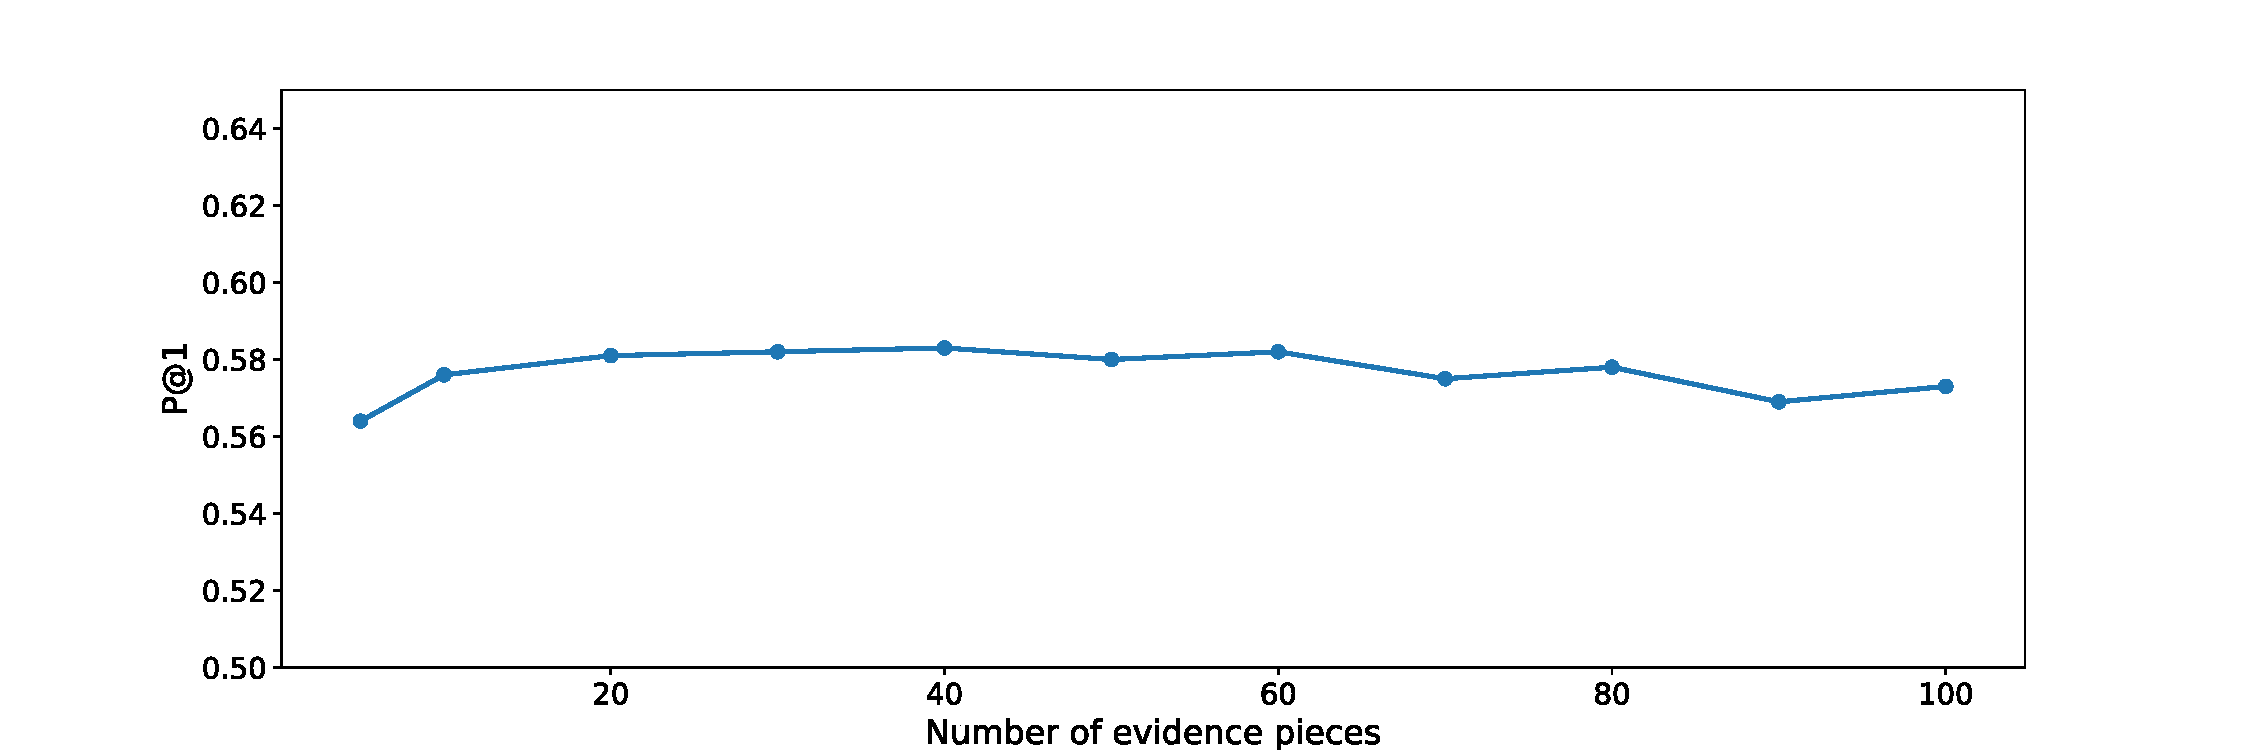
\includegraphics[width=0.8\textwidth]{submissions/Gerhard2024/figures/p_at_1-line_with_evidences.pdf}
    \vspace*{-0.2cm}
    \caption{Performance of \method on the \compmix dev set with different numbers of evidence.}
    \label{fig:res-num-evidences}
    \vspace*{-0.2cm}
\end{figure}



%%% ABLATION
\myparagraph{Ablation study on re-ranking} For more insight on the possible configurations of the RF stage, we conducted an ablation study with different options, including solely relying on the initial BM25 scoring without explicit re-ranking. The results are shown in Table \ref{tab:ablation2}. We observe that the iterative reduction in two steps is slightly better than the single-step variants (going down from top-1000 to top-30 in one RF step). Between the two options of using a GNN or a CE, the differences are negligible. A notable effect is that our RF techniques retain the answer presence at a very high level, only a bit lower than for the initial top-1000. 
The last two rows of Table \ref{tab:ablation2} demonstrate that RF is crucial: without explicit re-ranking, the technique of just picking smaller top-$k$ from the original BM25 model leads to substantial degradation in both answer presence and precision. 


\begin{table} [t] \small
    \centering
    \newcolumntype{G}{>{\columncolor [gray] {0.90}}c}
    \newcolumntype{H}{>{\setbox0=\hbox\bgroup}c<{\egroup}@{}}
    	\begin{tabular}{l G H G G G} 
        \toprule
            & \multicolumn{5}{G}{\textbf{\compmix} (dev set)} \\
        \midrule
            \textbf{RF Method $\downarrow$ / Metric $\rightarrow$} & \textbf{P@1} & \textbf{AP@1000} & \textbf{AP@100}  & \textbf{AP@30} & \textbf{MRR@100} \\ 
        \midrule
            \textbf{GNN: 1000 $\rightarrow$ 100 $\rightarrow$ 30}             &  $\mathbf{0.574}$  & $0.760$ &  $0.738$  &  $0.710$  &  $\mathbf{0.572}$  \\
            \textbf{CE: 1000 $\rightarrow$ 100 $\rightarrow$ 30}          &  $0.573$  & $0.760$  &   $\mathbf{0.740}$ &  $\mathbf{0.721}$   &  $0.553$   \\
        \midrule
            \textbf{GNN: 1000 $\rightarrow$ 30} &  $0.567$  & $?$  &   $n/a$ &  $0.710$   &  $0.567$   \\
         \textbf{CE: 1000 $\rightarrow$ 30} &  $0.570$  & $0.760$  &   $n/a$ &  $0.715$   &  $0.558$   \\
            \midrule
           \textbf{BM25: 100 (w/o GNN or CE)} &  $0.490$ & $0.760$  &  $0.652$  &  $n/a$  &  $0.259$ \\       
            \textbf{BM25: 30 (w/o GNN or CE)} &  $0.468$  & $0.760$  &  $n/a$ &  $0.534$   &  $0.259$   \\
            \bottomrule
    \end{tabular}
    \vspace*{-0.2cm}
    \caption{Ablation study for different RF strategies of \method on the \compmix dev set. The answer presence in the RF input with top-$1000$ evidence pieces is $0.760$.}
    \label{tab:ablation2}
\end{table}



\myparagraph{Quality of SI}
To assess the quality and robustness of the Structured Intents, we
inspected a sample of questions and their SIs.
Table~\ref{tab:question-SI-examples} gives three anecdotic examples.
We show SIs generated by \method, which makes use of the pre-existing collection from the \compmix benchmark for training.
This training data was obtained via different heuristics, 
which can be a limiting factor when user intents become more complex.

Therefore, we also looked at SIs derived via in-context learning (ICL) using \gptfour with $5$ handcrafted examples.
As shown in our earlier work on temporal QA~\cite{Jia-FAITH:WWW2024},
such data can be used for training smaller models (e.g., BART),
which can greatly boost the completeness and overall quality of the generated SIs.

From the sampled set, we observed that the ICL-based SIs are more
complete with all slots filled, whereas the BART-based SIs focused more
on the main slots Answer-type, Entities and Relation.
However, both approaches achieve very high quality in filling the slots,
capturing the user's information need very well.

Interestingly, when questions get complicated, with nested phrases, 
the ICL-based variant succeeds in decomposing the questions, based on only $5$ ICL examples.
For example, for the question {\em ``which German state had the most Corona-related death cases in the first year after the outbreak?''}
the Time slot becomes {\em ``first year after Corona outbreak''},
which can be resolved to identify the temporal scope.
In general, we believe that such question decomposition, beyond simple temporal constraints,
would be an interesting theme for future work.

\begin{table} [t] 
    \centering
    \small
    \newcolumntype{G}{>{\columncolor [gray] {0.90}}c}
    \newcolumntype{H}{>{\setbox0=\hbox\bgroup}c<{\egroup}@{}}
    \resizebox*{\textwidth}{!}{
        \begin{tabular}{p{6cm}|p{6cm}|p{6cm}} 
        \toprule
            \textbf{Question} & \textbf{Current SI by \method} & \textbf{SI via ICL} \\
        \midrule
        \textit{what was disneys first color movie?}
            & Ans-Type: \textit{animated feature film} & Ans-Type: \textit{film, animated film} \\
            & Entities: \textit{disneys} & Entities: \textit{Disney} \\
            & Relation: \textit{was first color movie} & Relation: \textit{first color movie} \\
            &  & Time: \textit{first} \\
        \midrule
        \textit{at the oscars, who won best actor in 2018?}
            & Ans-Type: \textit{human} & Ans-Type: \textit{person, actor} \\
            & Entities: \textit{at the oscars} & Entities: \textit{Oscars, 2018} \\
            & Relation: \textit{who won best actor in 2018} & Relation: \textit{won best actor} \\
            &  & Time: \textit{2018} \\
        \midrule
        \textit{which German state had the most Corona-} & Ans-Type: \textit{state} & Ans-Type: \textit{location, state} \\
        \textit{related death cases in the first year after} & Entities: \textit{Germany, Corona} & Entities: \textit{Germany, Corona-related deaths} \\
        \textit{the outbreak?} & Relation: \textit{which state had the most related} & Relation: \textit{highest count of death cases} \\
        & \textit{death cases in the first year after the out-}  & Location: \textit{Germany} \\
            & \textit{break}  & Time: \textit{first year after Corona outbreak} \\
        \bottomrule
    \end{tabular}
    }
    \vspace*{-0.2cm}
    \caption{Examples for pairs of question and generated SI.}
    \label{tab:question-SI-examples}
\end{table}




%%% REFRAIN FROM ANSWER
\myparagraph{Refraining from answering}
%%% Searched for: "generated_answer I" (with I being the full word, not partial) in the generated answers of LLaMA
%%% yields 245 results out of 2764 questions on CompMix
%%% yields 1270 results out of 3237 questions on TimeQuestions
We can train our model to refrain from answering in scenarios
where the provided evidence does not contain an answer to the question.
Specifically, during training, when the answer is not present in the evidence,
we change the target answer to {\em unknown}. This variant is referred to as \method {\em (faithful)}.

We measure the ratio of questions for which {\em unknown} is provided as answer,
and the P@1 restricted to questions that are answered.
The accuracy of refraining from answering is measured as well,
based on whether the answer is present in the evidence or not.
We conduct this experiment on \compmix and \timequestions,
for which we can compute answer presence exactly.
We also compute results for \llama, which is already instructed 
with the option to answer ``don't know''.
Table~\ref{tab:refrain-from-answer} shows the results.
For \compmix, we observe that \method has high accuracy on refraining when appropriate,
whereas \llama tends to be overconfident with a very small rate of {\em unknowns}, leading to incorrect answers.

\begin{table} [t] \small
    \centering
    \newcolumntype{G}{>{\columncolor [gray] {0.90}}c}
    \newcolumntype{H}{>{\setbox0=\hbox\bgroup}c<{\egroup}@{}}
    	\begin{tabular}{l G G G G c c c c} 
        \toprule
            & \multicolumn{4}{G}{\textbf{\compmix}} & \multicolumn{4}{c}{\textbf{\timequestions}} \\
            \midrule
            \textbf{Metric $\rightarrow$} & \textbf{P@1}  & \textbf{P@1} & \textbf{Refrain} & \textbf{Refrain} & \textbf{P@1}  & \textbf{P@1} & \textbf{Refrain} & \textbf{Refrain} \\ 
            \textbf{Method $\downarrow$} &                 & \textbf{(answered)} & \textbf{rate} & \textbf{accuracy} &                 & \textbf{(answered)} & \textbf{rate} & \textbf{accuracy} \\ 
            \midrule
                \textbf{\llama}             &  $0.431$  &  $0.471$  &  $0.089$  &  $n/a$  &  $0.177$  &  $0.276$  &  $0.392$  &  $n/a$  \\
                \textbf{\method (faithful)}           &  $0.497$  &  $0.713$  &  $0.303$  &  $0.838$ &  $0.597$  &  $0.804$  &  $0.257$  &  $0.864$  \\
            \bottomrule
    \end{tabular}
    \vspace*{-0.2cm}
    \caption{
        Performance of \method with option to refrain from answering (``don't know'').
    }
    \label{tab:refrain-from-answer}
\end{table}

\label{sec:disc}
\section{Insights, Limitations, and Challenges}


\noindent{\bf Benchmark Performance.} Our method, RAG-based \method with an 8B LLaMA model, outperforms much larger LLMs like \gptfour on two of the three benchmarks, with a very large margin for temporal questions. Obviously, pre-trained LLMs have only limited sense of properly positioning ``remembered’’ facts on the timeline even with training data that exceeds ours by several orders of magnitude. This confirms our intuition that LLMs alone are not good at ``recalling’’  higher-arity relations that require combining distant pieces of evidence. This is a sweet spot for RAG. Only for 
the \crag benchmark, \method is substantially inferior to a full-blown LLM. This is likely due to the nature of the questions: not necessarily the complexity of the information needs, but the need for more web sources (beyond what our experiments tap into).

\vspace{0.2cm}
\noindent{\bf Cost/Performance Ratio.} The most important take-away from our experiments is that \method achieves its competitive performance at a much lower cost than the full LLMs. Assuming that the consumed GFlops are proportional to the number of model parameters, \method achieves a cost reduction by a factor of 200x for \gptthree and 2000x for \gptfour. This does not only mean less computation, but also a massively lower electricity bill and climate impact.  

\vspace{0.2cm}
\noindent{\bf Role of Question Understanding.} We did not systematically investigate the influence of the Structured Intent in the \method pipeline. However, the comparison to the big GPT models reflects the role of the SI, as we prompt the GPT models in their natural mode with the original questions. The linearized sequence of available SI slots does not always have major advantages, but there are enough cases where specific facets provide crucial cues. This holds especially for the Entities slot, as this drives the gathering of evidence in the ER stage (cf.~\cite{Christmann-CONVINSE:SIGIR2022}, and for the Time slot, as these cues are often decisive for temporal questions (cf.~\cite{Jia-FAITH:WWW2024}).

\vspace{0.2cm}
\noindent{\bf Role of Re-Ranking.} As our ablation studies show, merely using top-$k$ evidence from an initial BM25-style ranking does not provide good performance. Also, there seems to be sweet spot in the choice of $k$: we need enough evidence for connecting the dots if the question requires multiple pieces of information, or for corroborating candidates if the question finds many useful but noisy pieces. In the experiments, $k=30$ turns out to be good choice; much lower $k$ results in insufficient evidence, and much larger $k$ leads to saturation and ultimately degrading performance. Our argument for iteratively shrinking the candidate set in multiple rounds of re-ranking is substantiated in our experiments, but the gain of doing this, compared to GNN- or CE-based re-ranking from 1000 to 30, is not big. More research is called to better understand the role of ranking in RAG. 

\vspace{0.2cm}
\noindent{\bf Limitations of Evidence Retrieval.}
For ER, we adopted more or less standard techniques. The results showed very good answer presence, in the order of 75\% in the top-100 or even top-30. An important case where this is insufficient are questions that require aggregating information over a large number of evidence pieces. An example is asking for the life-time total of 3-point scores of the basketball player Dirk Nowitzki.
This requires collecting a set of per-season tables with NBA player statistics, but also other web sources with numbers for his career before he joined the NBA (including his youth teams).
Of course, there are sometimes shortcuts like a Wikipedia article or biography mentioning the total number, but this cannot be universally assumed. The bottom line is that ER should be reconsidered as well, striving to improve the recall dimension.

\vspace{0.2cm}
\noindent{\bf Limitations of Answer Generation.}
For AG, we simply rely on a LLM,
using it as an extractor (``reader'') from the given evidence. Despite the wide belief that LLMs can perform deep
reasoning over many pieces of evidence, our experience is that the extraction works only well – robustly and faithfully – for relatively simple questions with a few multi-hop joins or simple aggregation over a few pieces. However, complicated questions such as asking for the top-100 NBA players with the largest number of life-time 3-point scores (again including their pre-NBA careers) are currently out of scope and will likely remain so for quite some time. This offers many opportunities for pushing the envelope further.

\vspace{0.2cm}
\noindent{\bf Trust in Data Sources.}
In our experiments, we considered all heterogeneous sources as trustworthy and unbiased. With focus on Wikidata and Wikipedia, this assumption has been well justified. In the wild, however, input data for RAG-based systems likely exhibit a wide spectrum of quality issues, in terms of stale information, biased positions, or simply false statements. Identifying trustworthy and up-to-date evidence and dealing with conflicting data, has been explored in other contexts (e.g., for KG curation~\cite{Dong-Trust:PVLDB2015}), but remains a major challenge for RAG-based QA.


\vspace{0.2cm}
\noindent{\bf Open Challenges and Future Work.} The best-performing methods in our experiment, mostly \method, reach P@1 values of 56\% for \compmix and 75\% for \timequestions. 
For the latter, the answer presence in the top-100 is only slightly higher; so the AG stage hardly misses anything.
However, for \compmix, the answer presence is 75\% -- much higher than what our system can actually answer. Obviously, closing this gap is a major direction to pursue, with focus on the RF and AG stages. However, missing one fourth of the answers completely in the top-100 pool, is a big problem as well. This requires improving recall at the ER stage, possibly with better guidance by the QU, which in turn needs more sources beyond the scope of our experiments (currently limited to Wikidata and Wikipedia). 

In general, we need to think beyond this kind of ``benchmark mindset’’. Even if we reached 80\% or 90\% precision and recall, we would still have a substantial fraction of questions that are answered incorrectly
or not at all. 
The remaining errors may not be a problem for chatbots, but they would be a showstopper for the deployment of mission-critical applications in business or science. We believe that this big gap is a shortcoming of {\em all methods}, not an issue that comes from the data alone. For trivia-style QA, as looked at in this paper, a smart human in ``open book’’ mode and no time limitation should be able to properly answer practically all questions, just by reading pieces of web contents and putting things together. Neither LLMs nor state-of-the-art RAG are the final solution; substantial research and creative ideas are needed to further advance QA.


\clearpage
\newpage

\newcommand{\bibauthors}[1]{{#1}}
\newcommand{\bibtitle}[1]{\emph{#1}}
\newcommand{\bibconf}[1]{{#1}}

\begin{thebibliography}{10}

\bibitem{Bajaj:arxiv2018}
\bibauthors{Payal Bajaj, Daniel Campos, Nick Craswell, Li Deng, Jianfeng Gao, Xiaodong Liu, Rangan Majumder, Andrew McNamara, Bhaskar Mitra, Tri Nguyen, Mir Rosenberg, Xia Song, Alina Stoica, Saurabh Tiwary, Tong Wang.}
\bibtitle{MS MARCO: A Human Generated MAchine Reading COmprehension Dataset.}
In \bibconf{arXiv 2018}.

\bibitem{DBLP:conf/acl/ChenFWB17}
\bibauthors{Danqi Chen, Adam Fisch, Jason Weston and Antoine Bordes.}
\bibtitle{Reading Wikipedia to Answer Open-Domain Questions.}
In \bibconf{ACL 2017}.

\bibitem{Christmann-CONVINSE:SIGIR2022}
\bibauthors{Philipp Christmann, Rishiraj Saha Roy, Gerhard Weikum.}
\bibtitle{Conversational Question Answering on Heterogeneous Sources.}
In \bibconf{SIGIR 2022}.

\bibitem{Christmann-CLOCQ:WSDM2022}
\bibauthors{Philipp Christmann, Rishiraj Saha Roy, Gerhard Weikum.}
\bibtitle{Beyond NED: Fast and Effective Search Space Reduction for Complex Question Answering over Knowledge Bases.}
In \bibconf{WSDM 2022}.

\bibitem{Christmann-Explaignn:SIGIR2023}
\bibauthors{Philipp Christmann, Rishiraj Saha Roy, Gerhard Weikum.}
\bibtitle{Explainable Conversational Question Answering over Heterogeneous Sources via Iterative Graph Neural Networks.}
In \bibconf{SIGIR 2023}.

\bibitem{Christmann-CompMix:WWW2024}
\bibauthors{Philipp Christmann, Rishiraj Saha Roy, Gerhard Weikum.}
\bibtitle{CompMix: A Benchmark for Heterogeneous Question Answering.}
In \bibconf{WWW 2024}.

\bibitem{Dejean:arxiv2024}
\bibauthors{Herve Dejean, Stephane Clinchant, Thibault Formal.}
\bibtitle{A Thorough Comparison of Cross-Encoders and LLMs for Reranking SPLADE.}
In \bibconf{arXiv 2024}.

\bibitem{Dhingra-time-aware-LLM:TACL2022}
\bibauthors{Bhuwan Dhingra, Jeremy R Cole, Julian Martin Eisenschlos, Daniel Gillick, Jacob Eisenstein, and William W Cohen.}
\bibtitle{Time-Aware Language Models as Temporal Knowledge Bases.}
In \bibconf{TACL 2022}.

\bibitem{Dong-Trust:PVLDB2015}
\bibauthors{Xin Luna Dong, Evgeniy Gabrilovich, Kevin Murphy, Van Dang, Wilko Horn, Camillo Lugaresi, Shaohua Sun, Wei Zhang.}
\bibtitle{Knowledge-Based Trust: Estimating the Trustworthiness of Web Sources.}
In \bibconf{PVLDB 2015}.

\bibitem{DBLP:journals/arXiv/abs-2312-10997}
\bibauthors{Yunfan Gao, Yun Xiong, Xinyu Gao, Kangxiang Jia, Jinliu Pan, Yuxi Bi, Yi Dai, Jiawei Sun, Qianyu Guo, Meng Wang, Haofen Wang.}
\bibtitle{Retrieval-Augmented Generation for Large Language Models: A Survey.}
In \bibconf{arXiv 2023}.

\bibitem{Gao-citations:emnlp2023}
\bibauthors{Tianyu Gao, Howard Yen, Jiatong Yu, Danqi Chen.}
\bibtitle{Enabling Large Language Models to Generate Text with Citations.}
In \bibconf{EMNLP 2023}.

\bibitem{Guu-REALM:ICML2020}
\bibauthors{Kelvin Guu, Kenton Lee, Zora Tung, Panupong Pasupat, Ming-Wei Chang.}
\bibtitle{Retrieval Augmented Language Model Pre-Training.}
In \bibconf{ICML 2020}.

\bibitem{DBLP:conf/eacl/IzacardG21}
\bibauthors{Gautier Izacard, Edouard Grave.}
\bibtitle{Leveraging Passage Retrieval with Generative Models for Open Domain Question Answering.}
In \bibconf{EACL 2021}.

\bibitem{Jia-TimeQuestions}
\bibauthors{Zhen Jia, Soumajit Pramanik, Rishiraj Saha Roy, and Gerhard Weikum.}
\bibtitle{Complex Temporal Question Answering on Knowledge Graphs.}
In \bibconf{CIKM 2021}.

\bibitem{Jia-FAITH:WWW2024}
\bibauthors{Zhen Jia, Philipp Christmann, Gerhard Weikum.}
\bibtitle{Faithful Temporal Question Answering over Heterogeneous Sources.}
In \bibconf{WWW 2024}.

\bibitem{DBLP:journals/arXiv/abs-2305-06984}
\bibauthors{Ehsan Kamalloo, Nouha Dziri, Charles L. A. Clarke, Davood Rafiei.}
\bibtitle{Evaluating Open-Domain Question Answering in the Era of Large Language Models.}
In \bibconf{arXiv 2023}.

\bibitem{Kandpal:ICML2023}
\bibauthors{Nikhil Kandpal, Haikang Deng, Adam Roberts, Eric Wallace, Colin Raffel.}
\bibtitle{Large Language Models Struggle to Learn Long-Tail Knowledge.}
In \bibconf{ICML 2023}.

\bibitem{DBLP:conf/emnlp/KarpukhinOMLWEC20}
\bibauthors{Vladimir Karpukhin, Barlas Oguz, Sewon Min, Patrick S. H. Lewis, Ledell Wu, Sergey Edunov, Danqi Chen, Wen-tau Yih.}
\bibtitle{Dense Passage Retrieval for Open-Domain Question Answering.}
In \bibconf{EMNLP 2020}.

\bibitem{Lee-MATTER:ACL2024}
\bibauthors{Dongkyu Lee, Chandana Satya Prakash, Jack FitzGerald, Jens Lehmann.}
\bibtitle{MATTER: Memory-Augmented Transformer Using Heterogeneous Knowledge Sources.}
In \bibconf{ACL 2024}.

\bibitem{DBLP:conf/acl/LewisLGGMLSZ20}
\bibauthors{Mike Lewis, Yinhan Liu, Naman Goyal, Marjan Ghazvininejad, Abdelrahman Mohamed, Omer Levy, Veselin Stoyanov, Luke Zettlemoyer.}
\bibtitle{BART: Denoising Sequence-to-Sequence Pre-training for Natural Language Generation, Translation, and Comprehension.}
In \bibconf{ACL 2020}.

\bibitem{DBLP:conf/nips/LewisPPPKGKLYR020}
\bibauthors{Patrick S. H. Lewis, Ethan Perez, Aleksandra Piktus, Fabio Petroni, Vladimir Karpukhin, Naman Goyal, Heinrich Küttler, Mike Lewis, Wen-tau Yih, Tim Rocktäschel, Sebastian Riedel, Douwe Kiela.}
\bibtitle{Retrieval-Augmented Generation for Knowledge-Intensive NLP Tasks.}
In \bibconf{NeurIPS 2020}.

\bibitem{Lin:MC2021}
\bibauthors{Jimmy Lin, Rodrigo Frassetto Nogueira, Andrew Yates.}
\bibtitle{Pretrained Transformers for Text Ranking: BERT and Beyond.}
In \bibconf{Morgan \& Claypool Publishers 2021}.

\bibitem{Liu-SUQL:NAACL2024}
\bibauthors{Shicheng Liu, Jialiang Xu, Wesley Tjangnaka, Sina J. Semnani, Chen Jie Yu, Monica Lam.}
\bibtitle{SUQL: Conversational Search over Structured and Unstructured Data with Large Language Models.}
In \bibconf{NAACL-HLT 2024}.

\bibitem{Mavi:FnT2024}
\bibauthors{Vaibhav Mavi, Anubhav Jangra, Adam Jatowt.}
\bibtitle{Multi-hop Question Answering.}
In \bibconf{Foundations and Trends in Information Retrieval 2024}.

\bibitem{Minaee-LLM-survey}
\bibauthors{Shervin Minaee, Tomas Mikolov, Narjes Nikzad, Meysam Chenaghlu, Richard}
\bibtitle{Socher, Xavier Amatriain, and Jianfeng Gao.}
Large Language Models: A Survey.
In \bibconf{arXiv 2024}.

\bibitem{Nogueira:arxiv2019}
\bibauthors{Rodrigo Frassetto Nogueira, Kyunghyun Cho.}
\bibtitle{Passage Re-ranking with BERT.}
In \bibconf{arXiv 2019}.

\bibitem{Oguz-UniK-QA:NAACL2022}
\bibauthors{Barlas Oguz, Xilun Chen, Vladimir Karpukhin, Stan Peshterliev, Dmytro Okhonko, Michael Sejr Schlichtkrull, Sonal Gupta, Yashar Mehdad, Scott Yih.}
\bibtitle{UniK-QA: Unified Representations of Structured and Unstructured Knowledge for Open-Domain Question Answering.}
In \bibconf{NAACL-HLT 2022}.

\bibitem{RogersGA:CS2023}
\bibauthors{Anna Rogers, Matt Gardner, Isabelle Augenstein.}
\bibtitle{QA Dataset Explosion: A Taxonomy of NLP Resources for Question Answering and Reading Comprehension.}
In \bibconf{ACM Computing Surveys 2023}.

\bibitem{RoyAnand:MC2021}
\bibauthors{Rishiraj Saha Roy, Avishek Anand.}
\bibtitle{Question Answering for the Curated Web: Tasks and Methods in QA over Knowledge Bases and Text Collections.}
In \bibconf{Synthesis Lectures on Information Concepts, Retrieval, and Services, Morgan \& Claypool Publishers 2021}.

\bibitem{Pramanik-Uniqorn:JWS2024}
\bibauthors{Soumajit Pramanik, Jesujoba Alabi, Rishiraj Saha Roy, Gerhard Weikum.}
\bibtitle{UNIQORN: Unified Question Answering over RDF Knowledge Graphs and Natural Language Text.}
In \bibconf{Journal of Web Semantics 2024}.

\bibitem{Sun-PullNet:EMNLP2019}
\bibauthors{Haitian Sun, Tania Bedrax-Weiss, William W. Cohen.}
\bibtitle{PullNet: Open Domain Question Answering with Iterative Retrieval on Knowledge Bases and Text.}
In \bibconf{EMNLP/IJCNLP 2019}.

\bibitem{Sun:NAACL2024}
\bibauthors{Kai Sun, Yifan Ethan Xu, Hanwen Zha, Yue Liu, Xin Luna Dong.}
\bibtitle{Head-to-Tail: How Knowledgeable are Large Language Models (LLMs)? A.K.A. Will LLMs Replace Knowledge Graphs?}
In \bibconf{NAACL-HLT 2024}.

\bibitem{Touvron-LLaMA}
\bibauthors{Hugo Touvron, Thibaut Lavril, Gautier Izacard, Xavier Martinet, Marie-Anne Lachaux, Timothée Lacroix, Baptiste Rozière, Naman Goyal, Eric Hambro, Faisal Azhar, Aurelien Rodriguez, Armand Joulin, Edouard Grave, Guillaume Lample.}
\bibtitle{Llama: Open and efficient foundation language models.}
In \bibconf{arXiv 2023}.

\bibitem{Wu-STARK:arxiv2024}
\bibauthors{Shirley Wu, Shiyu Zhao, Michihiro Yasunaga, Kexin Huang, Kaidi Cao, Qian Huang, Vassilis N. Ioannidis, Karthik Subbian, James Zou, Jure Leskovec.}
\bibtitle{STaRK: Benchmarking LLM Retrieval on Textual and Relational Knowledge Bases.}
In \bibconf{arXiv 2024}.

\bibitem{Wu:IEEE2021}
\bibauthors{Zonghan Wu, Shirui Pan, Fengwen Chen, Guodong Long, Chengqi Zhang, Philip S. Yu.}
\bibtitle{A Comprehensive Survey on Graph Neural Networks.}
In \bibconf{IEEE Transactions on Neural Networks and Learning Systems 2021}.

\bibitem{Yang-CRAG}
\bibauthors{Xiao Yang, Kai Sun, Hao Xin, Yushi Sun, Nikita Bhalla, Xiangsen Chen, Sajal Choudhary, Rongze D. Gui, Ziran W. Jiang, Ziyu Jiang, Lingkun Kong, Brian Moran, Jiaqi Wang, Yifan Ethan Xu, An Yan, Chenyu Yang, Eting Yuan, Hanwen Zha, Nan Tang, Lei Chen, Nicolas Scheffer, Yue Liu, Nirav Shah, Rakesh Wanga, Anuj Kumar, Wen-tau Yih, Xin Luna Dong.}
\bibtitle{CRAG -- Comprehensive RAG Benchmark.}
In \bibconf{arXiv 2024}.

\bibitem{Yasunaga:NAACL2021}
\bibauthors{Michihiro Yasunaga, Hongyu Ren, Antoine Bosselut, Percy Liang, Jure Leskovec.}
\bibtitle{QA-GNN: Reasoning with Language Models and Knowledge Graphs for Question Answering.}
In \bibconf{NAACL-HLT 2021}.

\bibitem{Zhang-Spaghetti:ACL2024}
\bibauthors{Heidi C. Zhang, Sina J. Semnani, Farhad Ghassemi, Jialiang Xu, Shicheng Liu, Monica S. Lam.}
\bibtitle{SPAGHETTI: Open-Domain Question Answering from Heterogeneous Data Sources with Retrieval and Semantic Parsing.}
In \bibconf{ACL 2024}.

\bibitem{Zhang:NAACL2024}
\bibauthors{Jiahao Zhang, Haiyang Zhang, Dongmei Zhang, Yong Liu, Shen Huang.}
\bibtitle{End-to-End Beam Retrieval for Multi-Hop Question Answering.}
In \bibconf{NAACL-HLT 2024}.

\bibitem{Zhao-LLMsurvey}
\bibauthors{Wayne Xin Zhao, Kun Zhou, Junyi Li, Tianyi Tang, Xiaolei Wang, Yupeng Hou, Yingqian Min, Beichen Zhang, Junjie Zhang, Zican Dong, Yifan Du, Chen Yang, Yushuo Chen, Zhipeng Chen, Jinhao Jiang, Ruiyang Ren, Yifan Li, Xinyu Tang, Zikang Liu, Peiyu Liu, Jian-Yun Nie, Ji-Rong Wen.}
\bibtitle{A Survey of Large Language Models.}
In \bibconf{arXiv 2023}.

\bibitem{Zhao:arxiv2024}
\bibauthors{Penghao Zhao, Hailin Zhang, Qinhan Yu, Zhengren Wang, Yunteng Geng, Fangcheng Fu, Ling Yang, Wentao Zhang, Bin Cui.}
\bibtitle{Retrieval-Augmented Generation for AI-Generated Content: A Survey.}
In \bibconf{arXiv 2024}.

\bibitem{Zhu-ODQA-survey:arxiv2021}
\bibauthors{Fengbin Zhu, Wenqiang Lei, Chao Wang, Jianming Zheng, Soujanya Poria, Tat-Seng Chua.}
\bibtitle{Retrieving and Reading: A Comprehensive Survey on Open-domain Question Answering.}
In \bibconf{arXiv 2021}.

\end{thebibliography}


\end{document}

\end{article}
\begin{article}
{G-VARS: Towards Personalized Risk Assessments by Analyzing Gun Violence Susceptibility with Personal Knowledge Graphs}
{Dipkamal Bhusal, Sara Rampazzi, Michael Clifford, Nidhi Rastogi}
\setcounter{section}{0}
% Please don't change anything in the documentclass below:
% We recommend using these packages as below, but if you have a good reason and want to change these, you can.
\documentclass[11pt]{article}
\usepackage{deauthor}
\usepackage{tikz}
\usetikzlibrary{shapes,arrows.meta, positioning}
\usepackage{cite}
\usepackage{amsmath,amssymb,amsfonts}
\usepackage{graphicx}
\usepackage{textcomp}
\usepackage{xcolor}
\usepackage{booktabs}
\usepackage{subcaption}
\usepackage{soul}
\usepackage{float}
\usepackage{algpseudocode}
\usepackage{algorithm2e}  % Remove if you don't need algorithm2e
\usepackage{enumitem}
\usepackage{tikz}
\usepackage{blindtext}
\usepackage{hyperref}
\hypersetup{
    colorlinks=true,
    linkcolor=blue,
    filecolor=magenta,      
    urlcolor=cyan,
    pdftitle={Overleaf Example},
    pdfpagemode=FullScreen,
    }
\usepackage{url}


\urlstyle{same}


\begin{document}

\title{\textsf{G-VARS}: Towards Personalized Risk Assessments by Analyzing Gun Violence Susceptibility with Personal Knowledge Graphs}

% Submissions should be anonymized. See the CFP for details on how to anonymize your paper, including any references to your own work.
%\author{\em Anonymous Authors}

% The author information is skipped here, but can be used to include author information in the publication.
\author{Dipkamal Bhusal$^{1}$~~~~~~Sara Rampazzi$^{2}$~~~~~~Michael Clifford$^{3}$~~~~~~Nidhi Rastogi$^{1}$\\ \\
%Affiliation
$^1$Rochester Institute of Technology, NY, USA\\
$^2$University of Florida, FL, USA\\
$^3$Toyota InfoTech, CA, USA
}

\maketitle

\thispagestyle{plain}
\pagestyle{plain}

\begin{abstract}
Gun violence is a concerning issue in the United States and requires immediate societal attention for improved prediction and prevention. Prior approaches have often overlooked mental health, relying on static factors such as age, gender, and the criminal history of the crime perpetrator. These approaches frequently fail to consider the context and environmental factors contributing to an individual’s risk of gun violence. In this paper, we propose \textsf{G-VARS}, a framework based on personal knowledge graphs that aggregates public and personal information to assess and evaluate individuals for potential gun violence. \textsf{G-VARS} comprises three phases: data collection, personal knowledge graph generation, and personalized risk assessment and intervention planning. We also present a case study where we apply the \textsf{G-VARS} framework to assess the risk of gun violence among urban youth.

\end{abstract}

\section{Introduction}
Gun violence is a critical public health issue in the United States. In 2023, the US broke the record for the maximum number of mass shootings in a year \cite{michael_2023}. According to the Centers for Disease Control and Prevention (CDC), approximately 48,000 gun-related deaths occurred in 2022, which averages to 132 people dying from a firearm-related injury each day~\cite{CDC}. Predicting and preventing gun violence is a multifaceted challenge, and traditional risk assessment models have several limitations. For instance, prior approaches rely on static factors like age, gender, and criminal history of the crime perpetrator \cite{smith2020limitations} and frequently fail to consider the context and environmental factors contributing to an individual's risk of gun violence \cite{jones2019contextual}. Mental health factors are often overlooked, which misses the crucial role they play in risk assessment \cite{doe2021mental}. Additionally, prior approaches do not adapt to changing circumstances. To address these issues, there is a growing interest in more advanced, personalized, and dynamic approaches to gun violence risk assessment, such as machine learning and predictive analytics \cite{chen2020machine}, social media monitoring \cite{adams2019social}, mental health screening \cite{lee2020screening}, and community-based strategies \cite{harris2022community}.
\par
In this paper, we propose the Gun Violence Assessment and Risk Stratification (G-VARS) framework based on Personal Knowledge Graphs (PKG). A PKG is a structured, user-centric graph connected to nodes (also called entities) via edges (also called relations), which provide knowledge about an individual that is of personal importance~\cite{balog2019personal}. In the context of assessing risks from Gun Violence, a PKG is a structured representation of an individual's unique circumstances and risk factors, capturing the interplay between individual, social, and environmental factors, enabling the analysis of gun violence risk factors and the development of personalized risk assessments. \textsf{G-VARS} can be utilized by various stakeholders, including healthcare providers can use it to evaluate potential violence risks, while law enforcement agencies can use it for risk identification and intervention planning. It can also help in fighting the inflow of illicit weapons used in crimes. Policymakers can leverage \textsf{G-VARS} for data-driven insights into the root causes of gun violence, informing policy decisions. Research institutions can utilize it to understand gun violence factors and develop prevention strategies. Lastly, community organizations can use \textsf{G-VARS} to create tailored interventions based on specific risk factors. The actual implementation of \textsf{G-VARS} is no trivial task, and we answer some of these challenges in this paper through detailed planning and considerations, especially related to ethical and privacy aspects. We envision that the \textsf{G-VARS} will have the following use cases:
\newline
\textit{(1) Identifying individuals at high risk of gun violence}: The PKG can be used to identify individuals who are at high risk of perpetrating or being a victim of gun violence. This information can then be used to intervene with these individuals and provide them with the support they need.
\newline
\textit{(2) Developing targeted interventions}: The PKG can be used to develop targeted interventions for individuals at high risk of gun violence. These interventions can include mental health treatment, substance abuse treatment, and violence prevention programs.
\newline
\textit{(3) Informing policy decisions}: The PKG can be used to inform policy decisions about gun violence prevention. For example, the PKG can be used to identify areas where there is a high risk of gun violence and to develop targeted interventions for those areas.

\subsection*{Privacy and Ethics Concerns}
Building and analyzing \textsf{G-VARS} is a complex task. Aggregating personal, familial, and social data with health information raises significant privacy and ethical concerns. Consequently, finding and collecting sufficient data for predictions while upholding ethical and legal frameworks presents a significant challenge \cite{lee2016ethical,nissenbaum2020protecting,ieee_privacy,USCommerce}. However, advancements in privacy research and increased collaboration between governments, healthcare institutions, and other stakeholders offer a promising path forward. 
For instance, the Open Knowledge Network (OKN) initiative by the NSF \cite{nsf_proto_okn_nsf23571,okn_2022}, an interconnected network of knowledge graphs, could provide a crucial public data infrastructure to facilitate an AI-driven future. This network would enable the integration of diverse data necessary for the development of solutions to drive sustained economic growth, broaden opportunities, and tackle complex problems ranging from climate change to social equity. Addressing gun violence is a principal theme of this initiative. In conjunction with this, the National Institute of Justice (NIJ)\cite{nij_gun_violence} is endeavoring to develop a comprehensive database for nonfatal firearm injuries to inform evidence-based prevention policies and demonstrate efforts toward building a data infrastructure for AI-driven solutions. This paper operates under the assumption that such a knowledge network will be operational in the near future, paving the way for exciting research directions that will benefit society.

\section{Background and Related Work}\label{sec:background}
\subsection{Personal Knowledge Graphs (PKG)}
A Personal Knowledge Graph (PKG) is a resource of structured information about entities personally related to an individual, its attributes, and the relations between them \cite{balog2019personal} (see Figure \ref{fig:pkg}). Using this format, a PKG organizes an individual's personal data, including education, work history, hobbies, relationships, and preferences, into a structured format \cite{rastogi2020personal}. It connects these elements, highlighting relationships and patterns, to create a comprehensive overview of an individual's knowledge and experiences. In the context of this paper, a PKG is a structured representation of an individual's unique circumstances and risk factors, capturing the interplay between individual, social, and environmental factors, enabling the analysis of gun violence risk factors and the development of personalized risk assessments. We can leverage a PKG for personalized risk assessments by integrating and analyzing relevant data points such as an individual's mental health history, social connections, geographic location, and exposure to violence \cite{rastogi2020personal} within the context of gun violence risk factors. This analysis can further provide insights into an individual's susceptibility to gun violence. Using machine learning algorithms, we can then process this data to generate risk assessments that are more accurate and context-aware, enabling targeted interventions and prevention strategies tailored to the individual's unique circumstances.

\begin{figure}[h]
\small
\centering
\resizebox{1\columnwidth}{!}{
\begin{tikzpicture}[node distance=2cm, auto]

  % PKG 1
  \node[circle, draw, minimum size=0.75cm] (PKG1) {Person 1};
  \node[rectangle, draw, below left of=PKG1] (Social1) {Social 1};
  \node[rectangle, draw, below right of=PKG1] (Social2) {Social 2};
  \node[diamond, draw, minimum size=0.35cm, above left of=PKG1] (Behavior1) {B1};
  \node[diamond, draw, minimum size=0.35cm, above right of=PKG1] (Behavior2) {B2};
  \node[rounded rectangle, draw, left of=PKG1] (Context1) {Context 1};
  \node[rounded rectangle, draw, right of=PKG1] (Context2) {Context 2};

  \draw[->] (PKG1) -- (Social1);
  \draw[->] (PKG1) -- (Social2);
  \draw[->] (PKG1) -- (Behavior1);
  \draw[->] (PKG1) -- (Behavior2);
  \draw[->] (PKG1) -- (Context1);
  \draw[->] (PKG1) -- (Context2);

  % PKG 2
  \node[circle, draw, minimum size=0.75cm, right=5cm of PKG1] (PKG2) {Person 1};
  \node[rectangle, draw, below left of=PKG2] (Social3) {Social 3};
  \node[rectangle, draw, below right of=PKG2] (Social4) {Social 4};
  \node[diamond, draw, minimum size=0.35cm, above left of=PKG2] (Behavior3) {B3};
  \node[diamond, draw, minimum size=0.35cm, above right of=PKG2] (Behavior4) {B4};
  \node[rounded rectangle, draw, left of=PKG2] (Context3) {Context 3};
  \node[rounded rectangle, draw, right of=PKG2] (Context4) {Context 4};

  \draw[->] (PKG2) -- (Social3);
  \draw[->] (PKG2) -- (Social4);
  \draw[->] (PKG2) -- (Behavior3);
  \draw[->] (PKG2) -- (Behavior4);
  \draw[->] (PKG2) -- (Context3);
  \draw[->] (PKG2) -- (Context4);

  % Connecting edge between Context 2 of PKG 1 and Context 3 of PKG 2
  \draw[<->,dashed] (Context2) -- (Context3);

\end{tikzpicture}
}
\caption{Personal Knowledge Graphs of Person 1 \& Person 2 and their different components. \textit{Social} nodes symbolize social networks relevant to each PKG. \textit{Behavioral} nodes (B1, B2) indicate behavior patterns for each person. \textit{Context} nodes are the environmental, situational factors influencing each person. Person 1 \& 2 are connected due to overlapping context.}
\label{fig:pkg}
\end{figure}


\subsection{Limitations of Traditional Risk Assessment Models for Gun Violence}
\textbf{Data-Driven Limitations:} One set of limitations involves the data-driven aspects of these models. Traditional approaches often rely on static variables such as age, gender, and criminal history for risk assessment, which may lead to low predictive accuracy \cite{smith2020limitations}. Furthermore, these models tend to overlook contextual factors, including socioeconomic status, access to firearms, and exposure to community violence, which are crucial in assessing an individual's risk \cite{jones2019contextual}. Additionally, mental health considerations, although significant contributors to violence, are inadequately incorporated into these models \cite{doe2021mental}. Moreover, bias and discrimination are concerns, as these models may disproportionately affect certain demographic groups, leading to over-policing and inequities in the criminal justice system \cite{Lum_2016}. Finally, the inability of traditional models to predict rare events, such as gun violence by individuals with no prior violent history, poses significant challenges gun violence among certain demographic groups, such as people of color or those with mental health diagnoses \cite{Lum_2016}.\\
\textbf{Lack of consideration for protective factors:} Traditional risk assessment models often focus on identifying and assessing risk factors, but they may not adequately consider the role of protective factors. Protective factors are characteristics or circumstances that can reduce the likelihood of gun violence, such as strong social support, access to mental health care, or participation in positive activities \cite{Kovacs_2019}.\\
\textbf{Limited predictive accuracy:} Traditional risk assessment models have shown limited predictive accuracy, meaning that they are not always able to accurately identify individuals who are at risk of committing gun violence. This lack of accuracy can lead to both false positives (individuals who are incorrectly identified as being at risk) and false negatives (individuals who are at risk but are not identified by the model) \cite{Fazel_2020}.\\
\textbf{Operational Challenges:} Operational limitations also plague traditional risk assessment models. These models typically offer static assessments that do not adapt to changing circumstances or behaviors \cite{smith2020limitations,jones2019contextual}. Data sharing among various agencies and organizations is often limited, hindering the development of comprehensive risk assessment models \cite{Johnson_2019}. Privacy concerns arise when sensitive data is collected and shared for risk assessment, necessitating a balance between public safety and privacy rights \cite{Johnson_2019}. Resource constraints further limit scalability, as these models require substantial resources for effective implementation \cite{Davis_2020}. Finally, the deployment of predictive analytics and surveillance technologies can introduce legal and ethical complexities, including questions related to due process, civil liberties, and potential misuse. Addressing these limitations necessitates a transition towards more advanced, personalized, and context-aware approaches to gun violence risk assessment.


\subsection{Personal Knowledge Graphs for Personalized Risk Assessment}
Personal knowledge graphs (PKGs) offer a promising avenue for personalized risk assessment~\cite{Brown2018}. PKGs are representations of an individual's social, behavioral, and contextual information, capturing their unique relationships and experiences~\cite{jones2019contextual}. By analyzing PKGs, researchers can extract dynamic risk factors that may not be readily captured by traditional methods~\cite{jones2019contextual}. A growing body of research has explored the use of PKGs for risk assessment in various domains, including criminal justice~\cite{Brown2018}, child welfare~\cite{jones2019contextual}, and healthcare. These studies have demonstrated the potential of PKGs to identify individuals at high risk of recidivism~\cite{Brown2018}, child maltreatment~\cite{jones2019contextual}, and disease exacerbations. Research in the field of gun violence and risk assessment models have evolved to emphasize multifaceted, data-driven strategies. Studies supported by the National Institute of Justice (NIJ) highlight the effectiveness of such approaches in reducing gun trafficking and shootings \cite{nij2021}. Particularly noteworthy is the research on youth firearm involvement in New York City, revealing that fear and the desire for physical safety, more than criminal intent, drive young people to carry and use firearms \cite{nij2021youth}. Furthermore, studies have examined the transition from youth firearm involvement to adult criminal behaviors, offering insights into the long-term impacts of early exposure to gun violence \cite{nij2021delinquent}.

\subsection{Previous Studies on Graph Link Prediction}
Graphs are often used to model the complex network structures of real-world systems \cite{kazemi2018simple,ding2022data}. In these graphs, each node can develop various types of relationships (edges) with other nodes \cite{nasiri2022impact}. Predicting these nodes and their relationships is a key area of research, offering significant insights for diverse applications \cite{cen2019representation,kumar2022link,wang2021self,10004751}. Current methods focus on learning the significance of a node and its one- and multi-hop neighbors in a heterogeneous network graph. These approaches include using a global feature generator for initial node representations \cite{cen2019representation, kumar2022link} and a localized, attention-driven method for fine-tuning specific subgraphs \cite{wang2021self}. Additionally, some methods utilize node centralities to understand a network’s local, quasi-local, and global structures \cite{kumar2022link}. Heterogeneous social networks, characterized by their diverse interaction types and missing links (edges), present challenges for the predictive performance of existing models. To address this, \cite{10004751} propose the MTTM (Multi-Type Transferable Method) for missing link prediction. This method leverages adversarial neural networks to maintain robustness against varying types of data. Furthermore, some strategies incorporate the causal relationship between the graph structure and links to capture essential factors for accurate missing link prediction \cite{zhao2022learning}.

\subsection{Limitations in Current Research}
Despite the promising potential of PKGs, limited studies have investigated the use of PKGs for gun violence risk assessment or have focused on relatively small sample sizes~\cite{Fazel} due to which the effectiveness of PKGs in predicting gun violence risk across diverse populations remains unclear~\cite{Fazel}. Theoretical generalizations about the circumstances leading to firearms violence are notably lacking \cite{nij2021gaps}. A gap we aim to fill is the application of PKGs in the context of gun violence risk assessment by providing a more nuanced understanding of individual susceptibilities to gun violence. Our study aims to address these gaps by conducting a comprehensive analysis of gun violence risk factors using PKGs. By leveraging a large and diverse dataset, our study aims to identify novel risk factors and develop a more accurate and personalized risk assessment model. The findings of our study have the potential to inform the development of effective gun violence prevention interventions.

%\section{Motivation}\label{sec:motivation}

%\section{Datasets for Studying Gun Violence}
\section{Proposed Framework}
In this paper, we propose ``\textsf{G-VARS}'' (\ul{G}un \ul{V}iolence \ul{A}ssessment and \ul{R}isk \ul{S}tratification) Framework that uses personal knowledge graphs to analyze gun violence and the associated risks. The framework is a systematic approach to leverage individual-specific data for more accurate risk assessments related to gun violence. The framework \textsf{G-VARS} encompasses three key phases: data collection and integration, PKG construction, and personalized risk assessment and intervention planning. \textsf{G-VARS} offers several advantages over traditional risk assessment approaches, such as capturing the unique circumstances and risk profiles of individuals, enabling more accurate and targeted risk assessments; providing a holistic view of an individual's risk factors, considering individual, social, and environmental factors; enabling continuous monitoring and risk assessment by dynamically updating the knowledge graph as new data becomes available, and informing the development of tailored interventions that address the specific risk factors of each individual. Next, we describe the three key phases of \textsf{G-VARS}:

\subsection*{Phase 1: Data Collection and Integration}
In the initial phase of the \textsf{G-VARS} framework, data collection and integration are paramount but will necessitate careful consideration of ethical, privacy, and legal concerns. While diverse data from medical records, social media activity (anonymized), historical records, and environment (collected as group statistics) will be gathered to construct individual profiles, informed consent, algorithmic bias, transparency, data security, and legal compliance will be performed wherever necessary. Recognizing these challenges and that not all data points will be available at all times, a subset of the data will be used to construct the PKGs. We extensively cover the ethical, privacy and legal challenges in Section \ref{ethics} The amalgamation of this multifaceted data forms the foundation for constructing Personal Knowledge Graphs (PKGs) to enhance gun violence risk assessments.

\begin{enumerate}
\item \textbf{Demographics}: Age, gender, location, and socioeconomic status can all play a role in the risk of gun violence \cite{OToole_2023,kegler2023notes}. For instance, studies have shown that gun violence disproportionately affects racial and ethnic minorities and is highly concentrated in a relatively small number of neighborhoods that have historically been under-resourced and racially segregated \cite{CDC_2023}. Men account for 86\% of all victims of firearm death and 87\% of firearm injuries \cite{edmund2022gun}. However collecting demographics should balance the need for data with the protection of individual rights and the responsible use of technology. By focusing on group statistics, utilizing anonymized data, and contextualizing individual data, we can gain valuable insights into violence patterns while ensuring a just and ethical approach to risk assessment.

\item \textbf{Behavioral Factors}: This includes past criminal behavior, substance abuse issues, or involvement in violent incidents \cite{efsgv_2020,wamser2021understanding}. Research suggests that individuals who have been victimized by a weapon as adolescents are between two and three times more likely to perpetuate firearm violence as adults \cite{Adolescent_gun_violence}. Also, those with access to a firearm during adolescence are far more likely to perpetuate firearm violence as an adult \cite{Adolescent_gun_violence}.

\item \textbf{Mental Health}: Information about a person's mental health history, including any diagnoses or treatments, can be relevant \cite{Ramchand2021-iz,Russell2022-kq,noauthor_2021-yq}. While mental illness contributes to only about 4\% of all violence, the contribution to gun violence is even lower \cite{noauthor_2021-yq}. However, suicide risk is indeed elevated among people with certain mental illnesses (e.g., schizophrenia, depression, borderline personality disorder, bipolar disorder, and anxiety disorders), but suicide among those with such diagnoses is still rare \cite{Ramchand2021-iz}. Important to note that concerns about potential bias, discrimination, and stigma necessitate careful handling of this information. 

\item \textbf{Access to Firearms}: Details about a person's access to firearms, such as ownership or proximity to others who own guns, can be crucial \cite{noauthor_2021-fg,Adolescent_gun_violence,noauthor_2022-qy}. Studies show that access to firearms doubles the risk of homicide \cite{noauthor_2022-qy}. Simply having a gun in one's home doubles the chance of dying by homicide and increases the likelihood of suicide death by over three-fold \cite{noauthor_2021-fg}.

\item \textbf{Social Networks}: The relationships and associations a person maintains can influence their risk level \cite{tracy2016transmission,Mcdonald2013-ji,papachristos2014network}. This can include family, friends, or affiliations with certain groups. A person's social network is a key predictor of whether an individual will become a victim of gun homicide, even more so than race, age, gender, poverty, or gang affiliation \cite{Mcdonald2013-ji,papachristos2014network}.

\item \textbf{Online Activity}: Public posts or interactions on social media platforms can provide insights into a person's state of mind or intentions \cite{Written_Bynbsp_Dr2023-zu}. Studies have suggested that social media has contributed to the rise and proliferation of gun violence across the country by encouraging imitative behaviors, provoking retaliative actions, and offering ``bragging rights'' in some online communities \cite{Written_Bynbsp_Dr2023-zu}. In addition, social media has made private information such as real-time locations, personal violent imagery and discourse, and gang threats and affiliations easily accessible to the public.
\end{enumerate}

\begin{figure}[h]
\small
\centering
\resizebox{1\columnwidth}{!}{
\begin{tikzpicture}[node distance=1.75cm, auto]

 % Central node 'Individual' as a circle
  \node[circle, draw] (Individual) {Individual};

  % Smaller diamond-shaped nodes for 'Mental Health', 'Substance Abuse', and 'Healthcare'
  \node[diamond, aspect=1, draw, minimum size=.5cm, below left of=Individual, xshift=-1cm, yshift=-1cm] (MentalHealth) {Mental Health};
  \node[diamond, aspect=1, draw, minimum size=.5cm, below right of=Individual, xshift=1cm, yshift=-1cm] (SubstanceAbuse) {Substance Abuse};
  \node[diamond, aspect=1, draw, minimum size=.5cm, above left of=Individual, xshift=-2cm] (Healthcare) {Healthcare Access};

  % Curved rectangle-shaped nodes for 'Firearms' and 'Criminal History'
  \node[rectangle, rounded corners, draw, below of=Individual, yshift=-1cm] (CriminalHistory) {Criminal History};
  \node[rectangle, rounded corners, draw, right of=Individual, xshift=1cm] (FirearmsAccess) {Firearms Access};

  % Rectangle-shaped nodes for 'Family', 'Friends', 'Social Ties', and 'Neighborhood'
  \node[rectangle, draw, above right of=Individual, xshift=2cm] (Family) {Family};
  \node[rectangle, draw, right of=Family, xshift=1cm] (Friends) {Friends};
  \node[rectangle, draw, right of=Friends, xshift=1cm] (SocialTies) {Social Ties};
  \node[rectangle, draw, right of=Healthcare, xshift=2cm] (Neighborhood) {Neighborhood};

  % Edges representing relationships
  \draw[->] (Individual) -- (MentalHealth);
  \draw[->] (Individual) -- (SubstanceAbuse);
  \draw[->] (Individual) -- (CriminalHistory);
  \draw[->] (Individual) -- (Family);
  \draw[->] (Individual) -- (Friends);
  \draw[->] (Individual) -- (SocialTies);
  \draw[->] (Individual) -- (Neighborhood);
  \draw[->] (Individual) -- (Healthcare);
  \draw[->] (Individual) -- (FirearmsAccess);

\end{tikzpicture}}
\caption{PKG Construction in the context of gun violence risk assessment. It incorporates Individual Factors, Social Factors, and Community Factors.}
\label{fig:pkg-construction}
\end{figure}

\subsection*{Phase 2: PKG Construction}
The construction of Personal Knowledge Graphs (PKGs) includes entities such as individuals, family members, friends, community factors, and risk factors are represented as nodes within the PKG (see Figure \ref{fig:pkg-construction}). Relationships are the connections, interactions, and influence among these entities. For instance, the individual is linked to family members, friends, community factors, and risk factors, allowing for a comprehensive representation of their social and environmental context. To attribute significance to relationships, weights are assigned based on their relative importance in predicting gun violence risk; for example, strong connections to known gang members carry higher weights than distant ties to casual acquaintances. This phase transforms raw data into a structured, interconnected graph that forms the basis for subsequent personalized risk assessments.

\textbf{Identify Entities: }The nodes in the personalized knowledge graph (PKG) represent the various entities that contribute to an individual's risk of gun violence. Therefore, the first step is to identify the entities that will be part of PKG. In the context of gun violence risk assessment, these entities can be further categorized into three main groups: (1) \textit{Individual Factors}: These nodes represent the individual's personal characteristics and background, including demographic factors (age, gender, race, ethnicity), mental health factors (diagnoses, treatment history, symptoms), substance abuse factors (types of substances used, frequency of use, treatment history), and criminal history factors (types of offenses, dates of offenses, legal consequences); (2) \textit{Social Factors}: These nodes represent the individual's social connections and environment, including family members, friends, and other social ties. The characteristics and risk factors associated with these relationships are also captured, such as exposure to violence, gang involvement, and social support networks; and (3) \textit{Community Factors}: These nodes represent the individual's community context and surroundings, including neighborhood crime rates, poverty levels, access to mental health care, and access to firearms. These factors can significantly influence an individual's risk of gun violence exposure or involvement.

\textbf{Define Relationships: }The edges in the PKG represent the connections and relationships between the various nodes. Therefore, next, we define the relationships between these entities, which can be categorized into four main types: (1) \textit{Direct Relationships}: These edges directly connect individuals to their family members, friends, and other social connections. They represent the immediate and tangible connections within an individual's social network; (2) \textit{Indirect Relationships}: These edges connect individuals to community factors, such as living in a high-crime neighborhood or having easy access to firearms. They represent the broader environmental and contextual factors that influence an individual's risk profile; 
(3) \textit{Influential Relationships}: These edges represent the strength and influence of relationships between nodes. Stronger relationships, such as close family bonds or involvement in influential social groups, carry more weight in the risk assessment process; and (4) 
\textit{Risk Factor Relationships}: These edges connect risk factors directly to individuals. Weights are assigned to these edges based on the relative importance of each risk factor in predicting gun violence risk. This allows the PKG to identify the most significant contributing factors to an individual's overall risk profile.

The collected data is finally structured in a graph format following the entities and relationships defined in the previous steps. Each entity becomes a node in the PKG, and each relationship becomes an edge connecting two nodes. Once the PKG is built, we can analyze it to identify patterns, assess risks, or generate insights (see Phase \ref{phase3}). The center of this personal knowledge graph, it would be the individual who is being assessed for the risk of gun violence\cite{ilkou2022personal}. All other entities (demographics, behavioral factors, mental health history, etc.) are connected to this central node, forming a ``spiderweb'' layout5. This allows for a personalized representation of data and interests- \cite{balog2019personal,ilkou2022personal,chakraborty2022personal}.



% (8) Integrating Siloed Personal Knowledge Graphs - Medium. https://dmccreary.medium.com/integrating-siloed-personal-knowledge-graphs-d0e68bd06685.
% (9) AI Knowledge Graph Generator | Taskade. https://www.taskade.com/generate/content/knowledge-graph.
% (10) undefined. https://doi.org/10.1145/nnnnnnn.nnnnnnn.
% (11) undefined. https://doi.org/10.1145/3341981.3344241.

\subsection*{Phase 3: Personalized Risk Assessment and Intervention Planning}\label{phase3}
This phase of the \textsf{G-VARS} framework focuses on personalized risk assessment and intervention planning. Machine learning algorithms can be used to analyze the PKG to generate a personalized risk score for each individual, indicating their likelihood of perpetrating or being a victim of gun violence. Key risk factors contributing to an individual's risk profile are identified through an analysis of node centrality and relationship weights within the PKG. This comprehensive understanding allows for the development of tailored intervention strategies, addressing the specific risk factors identified for each individual. These interventions may encompass mental health treatment \cite{chandak2023building}, substance abuse treatment, violence prevention programs, or community-based interventions, ensuring a context-aware and personalized approach to reducing gun violence susceptibility. Below, we provide some of the key types of analysis that can be performed on the PKG:

\begin{enumerate} [label=(\roman*)]
\item \textbf{Centrality Measure}: Centrality analysis aims to identify the most critical nodes within the PKG, which can provide insights into the most influential factors or entities contributing to gun violence risk. Common centrality measures include degree centrality, betweenness centrality, and eigenvector centrality. For gun violence risk assessment, this analysis helps pinpoint which individuals or community factors have the most significant impact on an individual's risk score \cite{yang2021research} as well as which key relationships or experiences might increase an individual’s susceptibility to gun violence.
\item \textbf{Community Detection}: Community detection algorithms identify clusters or groups of nodes within the PKG that exhibit higher connectivity among themselves compared to the rest of the graph. In the context of gun violence, this analysis can reveal groups of risk factors or entities that tend to co-occur, like a combination of environmental, social, and personal factors, shedding light on patterns of influence or common contexts contributing to gun violence susceptibility \cite{yang2021research}.
\item \textbf{Link Prediction}: Link prediction techniques forecast the likelihood of forming a relationship between two nodes in the PKG. In gun violence risk assessment, this analysis can be valuable for anticipating potential connections or risks. For example, it can predict the likelihood of an individual becoming affiliated with a high-risk group or network, aiding in proactive intervention strategies \cite{yang2021research}.
\item \textbf{Rule-based Reasoning}: Rule-based reasoning involves using predefined rules or logical statements to make inferences and extract new knowledge from the existing PKG. This approach allows for the incorporation of domain-specific knowledge and expert-defined rules into the risk assessment process, ensuring that important contextual information is considered \cite{sun2021generation}. For example, rules could be defined to identify individuals who meet specific criteria, such as a history of violence and access to firearms, and flag them for further evaluation or intervention.
\item \textbf{Distributed Representation-based Reasoning}: Distributed representation techniques encode the semantic information of entities and relations in the PKG into vector spaces. This enables more efficient and scalable reasoning, facilitating the exploration of complex relationships and patterns within the graph. In the context of gun violence risk assessment, this can aid in uncovering hidden connections and dependencies (non-linear relationships between entities) among risk factors \cite{chen2022overview}.
\item \textbf{Neural Network-based Reasoning}: Neural network-based reasoning leverages the power of deep learning models to capture intricate patterns and relationships within the PKG. These models can handle non-linear and complex interactions, making them suitable for exploring nuanced aspects of gun violence risk. They are particularly useful when dealing with large and heterogeneous data sources \cite{sun2021generation}.
\item \textbf{Mixed Reasoning}: Mixed reasoning combines multiple reasoning methods to leverage their respective strengths. This approach allows for a more comprehensive analysis of the PKG by accommodating various types of information and modeling techniques. It can enhance the accuracy and robustness of gun violence risk assessments by incorporating diverse sources of knowledge \cite{sun2021generation}. For example, rule-based reasoning could be used to capture known risk factors, while neural network-based reasoning could be used to identify novel patterns and relationships.
\item \textbf{Graph Convolutional Network (GCN)}: Graph convolutional networks (GCNs) are a novel approach to graph representation learning that extends the concept of convolution from images to graphs. Additionally, GCNs can effectively capture the local and contextual information within a graph, making them well-suited for generating personalized knowledge graphs for gun violence risk assessment. This can help us develop more personalized risk assessment models that consider the unique relationships and interdependencies between an individual's risk factors \cite{gentile2019personalized}. For example, GCNs can capture the relational structure of the graph and the attributes of the nodes, providing a powerful tool for risk assessment in the context of gun violence.
\end{enumerate}

The specific analysis techniques used depend on the nature of the data, the structure of the PKG, and the specific objectives of the analysis. Always consult with experts when designing such a system \cite{kejriwal2022knowledge,Slawski_2022,yang2021research,sun2021generation,safavi2019personalized,gong2021construction,munir2023integrated,chen2022overview,gentile2019personalized}.


\section{Case Study}\label{sec:experiment}
Urban areas often face a higher risk of gun violence, especially among young individuals. To address this issue, we apply the \textsf{G-VARS} framework to assess the risk of gun violence among urban youth. Our study leverages publicly available datasets combined with anonymized personal information collected as group statistics to demonstrate the framework's potential.

\subsection{Data Collection and Integration}

For Data collection, we utilize data from the Center for Disease Control and Prevention’s (CDC) Youth Risk Behavior Surveillance System (YRBSS), one of the nation’s largest and most comprehensive public health datasets on adolescent behavior. It includes information on mental health, substance abuse, and exposure to violence \cite{yrbss_2023}. The National Violent Death Reporting System (NVDRS) dataset, available using WISQARS \cite{cdc_2021}, contains information about violent deaths, including gun-related incidents, from multiple states in the U.S. It provides demographic details, circumstances of death and toxicology results while protecting the identity of individuals involved \cite{nvdrs_cdc_2023}. Additionally, we incorporate data from the Gun Violence Archive (GVA), Mother Jones Investigation, Everytown for Gun Safety, and the FBI’s Supplemental Homicide Report.
\par 
To effectively assess the risk of gun violence among urban youth using the \textsf{G-VARS} framework, a comprehensive range of data can potentially be collected from social media platforms, depending on their access. This includes:
\begin{enumerate}
    \item \textit{Facebook:} Using the Facebook Open Research and Transparency (FORT) Researcher Platform \cite{fort_platform_2023}, researchers can access publicly shared content on Facebook and Instagram. Analyzing text, keywords, and phrases used in posts and comments, particularly within relevant groups or pages, can reveal potential indicators of violence, suicidal ideation, or threats. Through the API, researchers have access to posts, comments, images, and videos, anonymized private messages, and content spread through likes and shares. Additionally, user activity data from page views, clicks, group memberships, and ad interactions can offer insights into user behavior. Likewise, anonymized social network data can reveal connections between users, page and group affiliations, and user interactions with third-party applications, allowing a comprehensive understanding of online activity and user relationships \cite{fort_researcher_api_2019}.
    \item \textit{Reddit}: The vast user-generated content and activity data of Reddit can serve as a significant resource for narrowing down potential perpetrators of gun violence. Researchers can uncover potential indicators of violence or threats by analyzing publicly posted content such as text, keywords, phrases, images, videos, and user engagement. User activity data, such as subreddit subscriptions, posting history, and community interactions, can provide insights into user interests, behavioral patterns, and social networks. Additionally, metadata (timestamps, locations, account information) can enhance contextual information about the user. Researchers can access the ``Reddit Search''\cite{reddit_search_API,proferes2021studying,medvedev2019anatomy} for publicly searchable posts and comments, ``Subreddit Archives''\cite{proferes2021studying} for historical data of specific communities, and the ``Research API and Reddit Research Partnerships''\cite{rocha2023passive} for anonymized data, alibi with stricter privacy controls.
    \item \textit{Telegram}: Data points from Telegram \cite{telegram} include posts, comments, and media within public channels and groups, interactions with bots related to weapons, violence, or extremist content, usernames, biographies, profile pictures, and metadata like timestamps, group memberships, and IP addresses. These can reveal indicators of violence, extremist ideology, potential threats, user interests, networks, identities, affiliations, and connections between users. The methods for data collection contain scraping public channels and groups using tools like Telethon \cite{telethon} or Python libraries, monitoring bots to collect data on user interactions and network connections, manually collecting data through the Telegram web interface, and, in rare cases, collaborating with Telegram under specific conditions to access limited data sets\cite{telegram_privacy,telegram_tos}.
    \item \textit{Twitter}: Before Twitter was acquired and rebranded as ``X'' by Elon Musk, researchers could access using academic API and analyze the vast user-generated content and activity data such as publicly posted tweets, retweets, replies, user interactions, profile information, and metadata like timestamps, geotags, and IP addresses. By studying these, one could uncover potential indicators of violence, extremist ideology, potential threats, user interests, networks, identities, affiliations, and connections between users. 

\end{enumerate}

NOTE: There are ethical and privacy concerns associated with collecting user data from social media platforms, just like other sources of data, and may require a legal expert or an ethicist when planning data collection. We discuss them in Section \ref{ethics}.

\subsection{\textsf{G-VARS} Construction}

With the collected data from NVDRS, YRBSS, and social media sources, we proceed to construct the \textsf{G-VARS}. In this phase, we represent entities such as individuals, family members, friends, mental health status, substance abuse, and neighborhood characteristics as nodes within the graph. Relationships are established based on demographic information, social connections, and behavioral patterns, reflecting the intricate web of factors contributing to gun violence susceptibility among urban youth. These relationships are weighted to account for their relative importance in predicting risk, ensuring that our graph accurately reflects the nuances of each individual's situation and context. Additionally, data from social media data is carefully designed to maintain privacy and anonymity (this part is left for future research) and is integrated with real data to provide a foundation for personalized gun violence risk assessments and intervention planning.
\par
The \textsf{G-VARS} (Gun Violence Assessment and Risk Stratification) framework centers around the ``individual urban youth'' at risk of gun violence, which is the central node of the PKG, and captures various contextual factors and risk influences.

\subsubsection*{Central Node} The central node within the \textsf{G-VARS} represents the \textbf{Individual} – the urban youth whose gun violence risk is under assessment. This central node forms the foundation of the knowledge graph and is connected to various other nodes, creating a holistic representation of the individual's context and risk factors.

\subsubsection*{Nodes}

1. \textbf{Individual}: The central node representing the urban youth.
2. \textbf{Family Members}: Nodes representing immediate and extended family members, capturing familial relationships and dynamics.
3. \textbf{Friends and Peers}: Nodes representing friends and peers within the urban youth's social network, reflecting social interactions and connections.
4. \textbf{Mental Health Status}: A node indicating the individual's mental health status, including any diagnosed conditions or mental health history.
5. \textbf{Substance Abuse}: A node indicating the individual's substance abuse history or involvement, if applicable.
6. \textbf{Neighborhood Characteristics}: Nodes representing various neighborhood characteristics, such as crime rates, poverty levels, access to mental health care, and accessibility to firearms. These nodes provide insights into the environmental context in which the individual resides.

\subsubsection*{Relationships}

1. \textbf{Family Relationships}: Relationships connecting the central node (\textbf{Individual}) to family members, capturing familial ties and dynamics, with varying weights based on relationship strength.
2. \textbf{Social Connections}: Relationships connecting the central node (\textbf{Individual}) to friends and peers, reflecting social interactions and connections, with varying weights based on the strength of the social relationship.
3. \textbf{Mental Health Influence}: Relationships connecting the central node (\textbf{Individual}) to the Mental Health Status node, indicating the influence of mental health on the individual's risk profile.
4. \textbf{Substance Abuse Influence}: Relationships connecting the central node (\textbf{Individual}) to the Substance Abuse node, indicating the influence of substance abuse on the individual's risk profile.
5. \textbf{Neighborhood Influence}: Relationships connecting the central node (\textbf{Individual}) to various Neighborhood Characteristics nodes, representing the influence of the neighborhood environment on the individual's risk factors, with variable weights based on significance.

\subsubsection*{Attributes}

Each node within the \textsf{G-VARS} may contain attributes that provide additional context and information. For example:
- The \textbf{Individual} node may include demographic attributes such as age, gender, and ethnicity.
- The \textbf{Mental Health Status} node may include information on specific mental health diagnoses and treatment history.
- The \textbf{Substance Abuse} node may contain details on the type and frequency of substance use.
- The \textbf{Neighborhood Characteristics} nodes may include quantitative data, such as crime rates and poverty levels, specific to the individual's neighborhood.

\subsubsection*{Graph Dynamics} The \textsf{G-VARS} is not a static graph but a dynamic one that can evolve over time. Relationships may strengthen or weaken, and attributes can change. The graph can adapt to new information and evolving risk factors, allowing for continuous updates and personalized risk assessments.


\subsection{Personalized Risk Assessment and Intervention Planning}

\subsubsection*{Analysis and Risk Assessment} Various analyses, including centrality measures, community detection, and link prediction, are applied to the \textsf{G-VARS}. This comprehensive analysis takes into account the rich dataset gathered during Phase 1 from sources such as the CDC's YRBSS, NVDRS, and anonymized user and group social media data. The goal of this analysis is to identify influential factors, community clusters, and potential risk connections within the urban youth population. By leveraging the relationships and attributes within the \textsf{G-VARS}, we gain insights into the complex web of risk factors that contribute to gun violence susceptibility among individuals.


\subsubsection*{Risk Prediction and Intervention Planning} Predictive models can be deployed to analyze the extensive \textsf{G-VARS} dataset and generate personalized gun violence risk scores for urban youth. 

\subsubsection*{Machine Learning Method: Random Forest Classifier}

\textbf{Scenario}: Let's consider an urban youth, John, who has undergone assessment using the \textsf{G-VARS} framework, and our goal is to predict his chances of committing gun violence.

\textbf{Data Input}: The \textsf{G-VARS} dataset contains information about John's demographics, social connections, mental health status, substance abuse history, and neighborhood characteristics. It also includes the weighted relationships between these nodes.

\noindent\textbf{Steps Involved}:

1. \textbf{Data Preprocessing}: We preprocess the data, handling missing values and encoding categorical features. The dataset is then split into training and testing sets.

2. \textbf{Feature Engineering}: We extract relevant features from the \textsf{G-VARS} graph, such as centrality measures (e.g., degree centrality), community memberships, and neighborhood characteristics.

3. \textbf{Model Training}: We train a Random Forest Classifier on the training data, using features extracted from the \textsf{G-VARS} dataset. The model learns to predict the risk of gun violence based on these features.

4. \textbf{Model Evaluation}: We evaluate the model's performance on the testing set, assessing its ability to accurately predict John's risk of gun violence.

5. \textbf{Risk Prediction}: After the model is trained and validated, it is applied to John's \textsf{G-VARS} data to generate a personalized risk score. This score indicates John's likelihood of being involved in gun violence.

6. \textbf{Intervention Planning}: Based on John's risk score, intervention strategies can be tailored to his specific needs. For instance, if John's risk score is high due to his social connections with known gang members (identified through the \textsf{G-VARS} relationships), an intervention plan may include targeted counseling and community support programs to steer him away from gang involvement.

\subsection{Rule-Based Method Example}

\subsubsection*{Rule-Based Method: Expert-defined rules for substance abuse intervention}

\textbf{Scenario}: Consider an urban youth, Sarah, who is assessed using the \textsf{G-VARS} framework, and one of her identified risk factors is substance abuse.

\textbf{Data Input}: Sarah's \textsf{G-VARS} data includes information about her substance abuse history, social connections, and mental health status.

\textbf{Steps}:

1. \textbf{Identification of Substance Abuse}: The \textsf{G-VARS} framework identifies that Sarah has a history of substance abuse, which is a risk factor for gun violence.

2. \textbf{Expert-Defined Rules}: A set of expert-defined rules is applied to Sarah's case. These rules state that if an individual is identified with a substance abuse history, they should be recommended for a substance abuse intervention.

3. \textbf{Intervention Planning}: Based on the rule outcome, an intervention plan is generated for Sarah. In her case, the plan may include enrolling her in a substance abuse treatment program, such as counseling or rehabilitation.

4. \textbf{Monitoring and Adaptation}: The intervention's effectiveness is monitored over time, and the \textsf{G-VARS} framework can adapt the intervention plan based on Sarah's progress. For example, if Sarah successfully completes the initial substance abuse program, the plan may evolve to focus on relapse prevention and community support.


\subsection{Ethical Considerations}\label{ethics}

In the pursuit of personalized risk assessments for gun violence susceptibility, upholding ethical principles and safeguarding the rights and well-being of individuals is paramount. This section outlines the ethical framework and measures adhered to throughout the study.

\subsubsection{Data Anonymization and Privacy Protection}

Stringent data anonymization and privacy protection measures are implemented to ensure the privacy and anonymity of study participants. These measures include:

\begin{itemize}
    \item \textbf{De-Identification}: Personally identifiable information (PII), such as names, addresses, and contact details, is systematically removed from all datasets. Unique identifiers are replaced with pseudonyms to prevent traceability to specific individuals.
    
    \item \textbf{Secure Data Storage}: Collected data, whether from public health sources, anonymized user and group social media data, or other relevant datasets, is securely stored on encrypted servers. Access is strictly controlled, with only authorized personnel permitted to handle and process the data.
    
    \item \textbf{Data Minimization}: The principle of data minimization is followed to collect only the minimum necessary data for research purposes. Irrelevant or excessive data is not retained, minimizing the risk of privacy breaches.
\end{itemize}

\subsubsection{Informed Consent for Social Media Data}

The use of social media data to model online interactions of urban youth is a pivotal aspect of this study. To ensure ethical compliance, informed consent is diligently obtained from all participants involved in generating the data. This consent encompasses:

\begin{itemize}
    \item \textbf{Transparency}: Participants receive clear and comprehensible information about the purpose of data generation, how their data will be utilized, and the safeguards in place to protect their privacy.
    
    \item \textbf{Voluntary Participation}: Participation in generating synthetic social media data is entirely voluntary. Individuals can opt in or out without facing any adverse consequences.
    
    \item \textbf{Anonymity}: Participants are assured that the synthetic data will not be used to trace back to their real identities or shared with third parties for non-research purposes.
\end{itemize}

\subsubsection{Sensitivity and Non-Discrimination}

The ethical framework of this study prioritizes sensitivity and the prevention of stigmatization and discrimination. Key considerations include:

\begin{itemize}
    \item \textbf{Bias Mitigation}: Rigorous steps are taken to ensure that analyses and risk assessments performed using the \textsf{G-VARS} framework are free from biases related to race, gender, ethnicity, or socio-economic status. Machine learning models undergo regular fairness and equity audits.
    
    \item \textbf{Equity-Centric Interventions}: Intervention plans developed based on personalized risk assessments are designed to be equitable and sensitive to the unique needs of each individual. They aim to provide support and assistance without perpetuating stereotypes or biases.
    
    \item \textbf{Community Engagement}: The research actively engages with the involved communities to gain insights into their perspectives, concerns, and preferences. This collaborative approach ensures that we respect the voices and agency of those affected by its findings.
\end{itemize}

In summary, ethical considerations are integral to maintaining the highest standards of integrity and respect for individuals' rights and dignity in this research endeavor. Striving for transparency, data privacy, sensitivity, and fairness ensures that the \textsf{G-VARS} framework contributes positively to gun violence prevention while safeguarding the well-being of all individuals involved. Ethical oversight and compliance with relevant guidelines and regulations remain top priorities throughout the study.


\section{Conclusion and Future Work}\label{sec:conclusion}
In this paper, we propose the \textsf{G-VARS}, the first framework that leverages Personal Knowledge Graphs (PKG) to present a novel and comprehensive approach to understanding and mitigating gun violence. Through the integration of anonymized and statistically gathered group data on social and environmental factors and minimal individual data \textsf{G-VARS} to provide a dynamic and personalized assessment of gun violence risk to or on an individual. Its application extends across various domains, supporting healthcare providers, law enforcement, policymakers, etc., in identifying high-risk individuals, developing targeted interventions, and informing decisions. The successful implementation of G-VARS, however, hinges on addressing significant privacy and ethical concerns, necessitating a careful balance between data utility and individual rights. This paper's exploration of \textsf{G-VARS} underscores the potential of data-driven approaches in transforming our understanding and response to gun violence, marking a significant step forward in public health and safety. For future research, initiatives like the Open Knowledge Network and the National Institute of Justice's efforts in developing comprehensive databases for firearm injuries promise to enhance our capabilities in AI-driven solutions, furthering the impact of frameworks like \textsf{G-VARS} in creating safer, more informed communities.

\bibliographystyle{IEEEtran}
\bibliography{eurosp-2023-template}

\end{document}

\end{article}
\begin{article}
{QALinkPlus: Text Enrichment with Q&A data}
{Yandong Sun, Yixuan Tang, Anthony K.H. Tung}
\setcounter{section}{0}
\documentclass{article}

\usepackage{deauthor}

\usepackage{latexsym}
\usepackage{graphicx}
\graphicspath{{./images/}}
\usepackage{booktabs} % for formal tables
\usepackage{color}  % for coloring text
\usepackage{amsmath}  % for aligning equations
\usepackage{subcaption}
\usepackage{caption}
\usepackage{tikz}
\usepackage{colortbl} % for color in tables
\usepackage{framed}
\usepackage{multirow}
\usepackage{multicol}
\usepackage{hyperref}
\usepackage{url}
\usepackage{balance}
\usepackage{verbatim}
\usepackage{cancel}
\usepackage{xspace} % for correcting space after macro commands
\usepackage{algorithm2e}
\usepackage{bbold} % for writing mathbb{1}
\usepackage{balance}
\usepackage{stmaryrd}
\usepackage{enumitem}
\usepackage{array} % package for hiding a column
\usepackage{bold-extra} % to enable textbf with textsc

% used for making text readable in document and .tex
% \setlength{\parindent}{0pt}

\newcommand{\struct}[1]{\texttt{\small #1}}
\newcommand{\utterance}[1]{\textit{#1}}
\newcommand{\phrase}[1]{\textit{``#1''}}

% \newcommand {\g}[1]{\textcolor[gray]{0.6}{#1}}

\newcommand{\drop}{\dag\xspace}

\newenvironment{Snugshade}[1][236,236,236]{
    \setlength{\itemsep}{0pt}
     \setlength{\parsep}{0pt}
     \setlength{\topsep}{0pt}
     \setlength{\partopsep}{0pt}
     \setlength{\leftmargin}{1.5em}
     \setlength{\labelwidth}{0em}
     \setlength{\labelsep}{0em} 
    \setlength{\parskip}{0pt}
    \definecolor{shadecolor}{RGB}{#1}
    \begin{snugshade}
}{
    \end{snugshade}
}


\newcommand{\method}{\textsc{Quasar}\xspace}
\newcommand{\benchmark}{\textsc{PerQA}\xspace}
\newcommand{\itemslist}[1]{$\langle$\struct{#1}$\rangle$}


\newcommand{\convinse}{\textsc{Convinse}\xspace}
\newcommand{\explaignn}{\textsc{Explaignn}\xspace}
\newcommand{\clocq}{\textsc{Clocq}\xspace}
\newcommand{\unikqa}{\textsc{UniK-Qa}\xspace}
\newcommand{\gptthree}{\textsc{Gpt-3}\xspace}
\newcommand{\gptfour}{\textsc{Gpt-4}\xspace}
\newcommand{\llama}{\textsc{Llama3}\xspace}
\newcommand{\spaghetti}{\textsc{Spaghetti}\xspace}


\newcommand{\compmix}{\textsc{CompMix}\xspace}
\newcommand{\timequestions}{\textsc{TimeQuestions}\xspace}
\newcommand{\crag}{\textsc{Crag}\xspace}


\newcommand{\squishlist}{
    \begin{list}{$\bullet$}{
        \setlength{\itemsep}{0pt}
	\setlength{\parsep}{3pt}
	\setlength{\topsep}{3pt}
	\setlength{\partopsep}{0pt}
	\setlength{\leftmargin}{1.5em}
	\setlength{\labelwidth}{1em}
	\setlength{\labelsep}{0.5em}
    }
}

\newcommand{\squishend}{
    \end{list}
}

\newcommand{\myparagraph}[1]{\vspace*{0.2cm}\noindent \textbf{#1}.}
\newcommand{\myparagraphnospace}[1]{\noindent \textbf{#1}.}

% \newcommand{\GW}[1]{\emph{{\color{blue} GW:#1}}}
% \newcommand{\PC}[1]{\emph{{\color{orange} PC: #1}}}
% \newcommand{\tocite}{{{\color{red} [CITE]}}}


\begin{document}

\title{RAG-based Question Answering \\ over Heterogeneous Data and Text}

\author{
Philipp Christmann,
Gerhard Weikum\\\\
Max Planck Institute for Informatics\\
Saarland Informatics Campus, Germany\\
\texttt{\{pchristm, weikum\}@mpi-inf.mpg.de}}

\maketitle

\section*{Abstract}
This article presents the \method system for question answering over unstructured text, structured tables, and knowledge graphs, with unified treatment of all sources.
The system adopts a RAG-based architecture, with a pipeline of evidence retrieval followed by answer generation, with the latter powered by a 
moderate-sized
language model.
Additionally and uniquely, \method
has components for question understanding, to derive crisper input for evidence retrieval, and for re-ranking and filtering the retrieved evidence before feeding the most informative pieces into the answer generation.
Experiments with three different benchmarks demonstrate the high answering quality of our approach, being on par with or better than large GPT models, while keeping the computational cost and energy consumption orders of magnitude lower.

\label{sec:intro}
\section{Introduction}

\noindent\textbf{Motivation and Problem.} The task of question answering, QA for short, arises in many flavors: factual vs. opinions, simple lookups vs. multi-hop inference, single answer vs. list of entities, 
direct answers vs. long-form, one-shot questions vs. conversations, and other varieties 
(see, e.g., surveys~\cite{RogersGA:CS2023,RoyAnand:MC2021}).
The state-of-the-art for this entire spectrum has been greatly advanced in the past decade. Most notably, incorporating deep learning into retriever-reader architectures (e.g.,~\cite{DBLP:conf/acl/ChenFWB17,DBLP:conf/eacl/IzacardG21,DBLP:conf/emnlp/KarpukhinOMLWEC20}) has boosted answering quality, and most recently, large language models (LLM)~\cite{Minaee-LLM-survey,Zhao-LLMsurvey} have pushed the envelope even further (e.g.,~\cite{DBLP:journals/arXiv/abs-2305-06984}).

% strengths and limitations of LLM for QA
Today’s LLMs alone are capable of accurately answering many \textit{factoid} questions, simply from their pre-trained parametric memory which latently encodes huge text corpora and other online contents.
However, this critically depends on the frequency of evidence in the underlying contents and the complexity of the information need. 
For example, 
asking for the {\em MVP of the 2024 NBA season} would easily return the correct answer Nikola Jokic, 
but asking for the {\em highest-scoring German NBA player} or the {\em MVP of the 2024 German basketball league} pose a big challenge.
The reason is that LLMs alone do not easily recall information about not so popular or even long-tail entities~\cite{Kandpal:ICML2023,Sun:NAACL2024},
and that they are mainly geared for direct look-ups as opposed to connecting multiple pieces of evidence~\cite{Mavi:FnT2024,Zhang:NAACL2024}.

% introduce RAG and discuss need for heterogeneous sources
\cite{DBLP:journals/arXiv/abs-2312-10997,Guu-REALM:ICML2020,DBLP:conf/nips/LewisPPPKGKLYR020,Zhao:arxiv2024}
known as RAG, address these bottlenecks. In addition to cleverly crafted prompts and few-shot examples, the LLM is provided with the top-ranked results of an explicit retrieval step, like web search or knowledge graph (KG) lookups. The former is often necessary for freshness of answers, and the latter may help with long-tail entities and also mitigate the notorious risk of hallucinations. Still, this generation’s RAG architectures are limited in how broad and how deep they tap into external sources. Popular AI assistants like Gemini or ChatGPT seem to primarily retrieve from the text of web pages (incl. Wikipedia articles), and academic research has additionally pursued knowledge augmentation by enhancing prompts with facts from large KGs (e.g., Wikidata).

An additional content modality that is still underexplored are {\em online tables}: a wide range of tabular data including HTML tables in web pages, spreadsheets and statistics, all the way to CSV and JSON datasets that are abundant on the Internet. There is prior work on joint support for text and KGs and for text and tables, but very little on all of these together -- some notable exceptions being~\cite{Christmann-CONVINSE:SIGIR2022,Christmann-Explaignn:SIGIR2023,Oguz-UniK-QA:NAACL2022,Zhang-Spaghetti:ACL2024}.


\noindent\textbf{Examples.} All three heterogeneous types of sources are crucial not only for answering different questions from different kinds of evidence, but also for combining multiple pieces of evidence of different modalities to infer correct and complete answers.
To 
illustrate
the need for tapping all sources, consider the following questions:

% \vspace*{0.2cm}
\begin{quote}
$Q1$: \utterance{Which Chinese basketballers have played in the NBA?}\\
 \indent $Q2$: \utterance{Who was the first Chinese NBA player?}\\
  \indent $Q3$: \utterance{Which Chinese NBA player has the most matches?}
\end{quote}
% \vspace*{0.2cm}

Q1 can be cast into querying a KG, but the list there is not necessarily complete and up-to-date, so additional evidence from text or tables would be desired. 
Q2 needs information about who played in which seasons, found only in web pages or sports-statistics tables. 
Finally, Q3 may be lucky in finding prominent textual evidence (e.g., in biographies, Wikipedia etc.), but this often faces divergent statements, and resolving contradictions needs to dive into more evidence. Besides, when textual evidence is rare and hard to find or not trustworthy enough, then information from multiple tables and text snippets may have to be aggregated (e.g., totals of per-season counts).
Some of this may perhaps become feasible for an industrial LLM’s RAG capabilities in the near future, but there are always harder scenarios by moving from Chinese NBA players deeper into the long tail, such as asking for {\em Lithuanian players in the German handball league}.

\vspace*{0.2cm}
\noindent\textbf{Approach and Contribution.} This paper presents a simple but powerful and versatile RAG system with unified access to text, KG and tables. We call our method {\em \method} 
(for Question Answering over Heterogeneous Sources with Augmented Retrieval).
Its architecture is relatively straightforward: all heterogeneous content is verbalized and indexed for retrieval; a retriever finds top-ranked results for the given question (from different source types), and these are fed into the LLM for answer generation. This is the unsurprising bird-eye’s view. Specific details that are key factors for the strong performance of \method are: 

\squishlist
\item[i)] automatically casting user questions into a structured representation of the information need, which is then used to guide 
\item[ii)] judicious ranking of search results, with multiple rounds of re-ranking and pruning, followed by
\item[iii)]	extracting faithful answers from an LLM in RAG mode, with answers grounded in tangible evidence.
\squishend


\vspace{0.2cm}
\noindent The paper presents experiments with three different benchmarks, covering various flavors of questions.
We focus on one-shot questions; conversational QA is out of scope here, but \method itself is well applicable to this case, too.
Our experiments demonstrate that our methods are competitive, on par with big GPT models and often better,
while being several orders of magnitude lower in computational and energy cost.
The experimental findings also highlight that question understanding, with structured representation of user intents, and iterative re-ranking of evidence are crucial for good performance.

Overall, our contribution lies in proposing a unified system architecture for RAG-based question answering over a suite of different data sources, with strong points regarding both effectiveness (i.e., answer quality)
and efficiency (i.e., computational cost).


\label{sec:background}
\section{Related Work}

The RAG paradigm came up as a principled way of enhancing LLM factuality incl. provenance and mitigating the risk of hallucination~\cite{Guu-REALM:ICML2020, DBLP:conf/nips/LewisPPPKGKLYR020}.
It is highly related to the earlier
retriever-reader architectures for QA~\cite{DBLP:conf/acl/ChenFWB17,DBLP:conf/emnlp/KarpukhinOMLWEC20}, especially when the reader uses the fusion-in-decoder method~\cite{DBLP:conf/eacl/IzacardG21,Oguz-UniK-QA:NAACL2022}.
Since its invention, RAG methodology has been greatly advanced, introducing a wide suite of extensions, such as batched inputs, interleaving retrieval and generation steps, and more (see the recent surveys~\cite{DBLP:journals/arXiv/abs-2312-10997,Zhao:arxiv2024}).

On question answering (QA), there is a vast amount of literature including a wealth of differently flavored benchmarks (see, e.g.,~\cite{RogersGA:CS2023}).
The case of interest here is QA over heterogeneous sources, tapping into both unstructured content and structured data. 
A variety of works has pursued this theme by combining knowledge graphs with text sources, using graph-based methods, neural learning and  language models (e.g.,~\cite{Pramanik-Uniqorn:JWS2024,Sun-PullNet:EMNLP2019,Yasunaga:NAACL2021}).

Most relevant for this article is the research on jointly leveraging all different sources: text, KGs, and tables (incl. CSV and JSON files). This includes  
the \unikqa system~\cite{Oguz-UniK-QA:NAACL2022},
the \spaghetti/SUQL project~\cite{Liu-SUQL:NAACL2024,Zhang-Spaghetti:ACL2024},
the \textsc{Matter} method~\cite{Lee-MATTER:ACL2024},
the STaRK benchmarking~\cite{Wu-STARK:arxiv2024},
and our own prior work
~\cite{Christmann-CONVINSE:SIGIR2022,Christmann-Explaignn:SIGIR2023} (without claiming exhaustiveness).
Out of these, we include \unikqa, \spaghetti and our own systems \convinse and \explaignn as baselines in the experimental evaluation.
Their architectures are similar to ours, but \unikqa and \spaghetti do not have our distinctive elements of
question understanding and iterative re-ranking (originally introduced in \explaignn~\cite{Christmann-Explaignn:SIGIR2023}).

\label{sec:method}
\section{Methodology}

\begin{figure}[tb]
  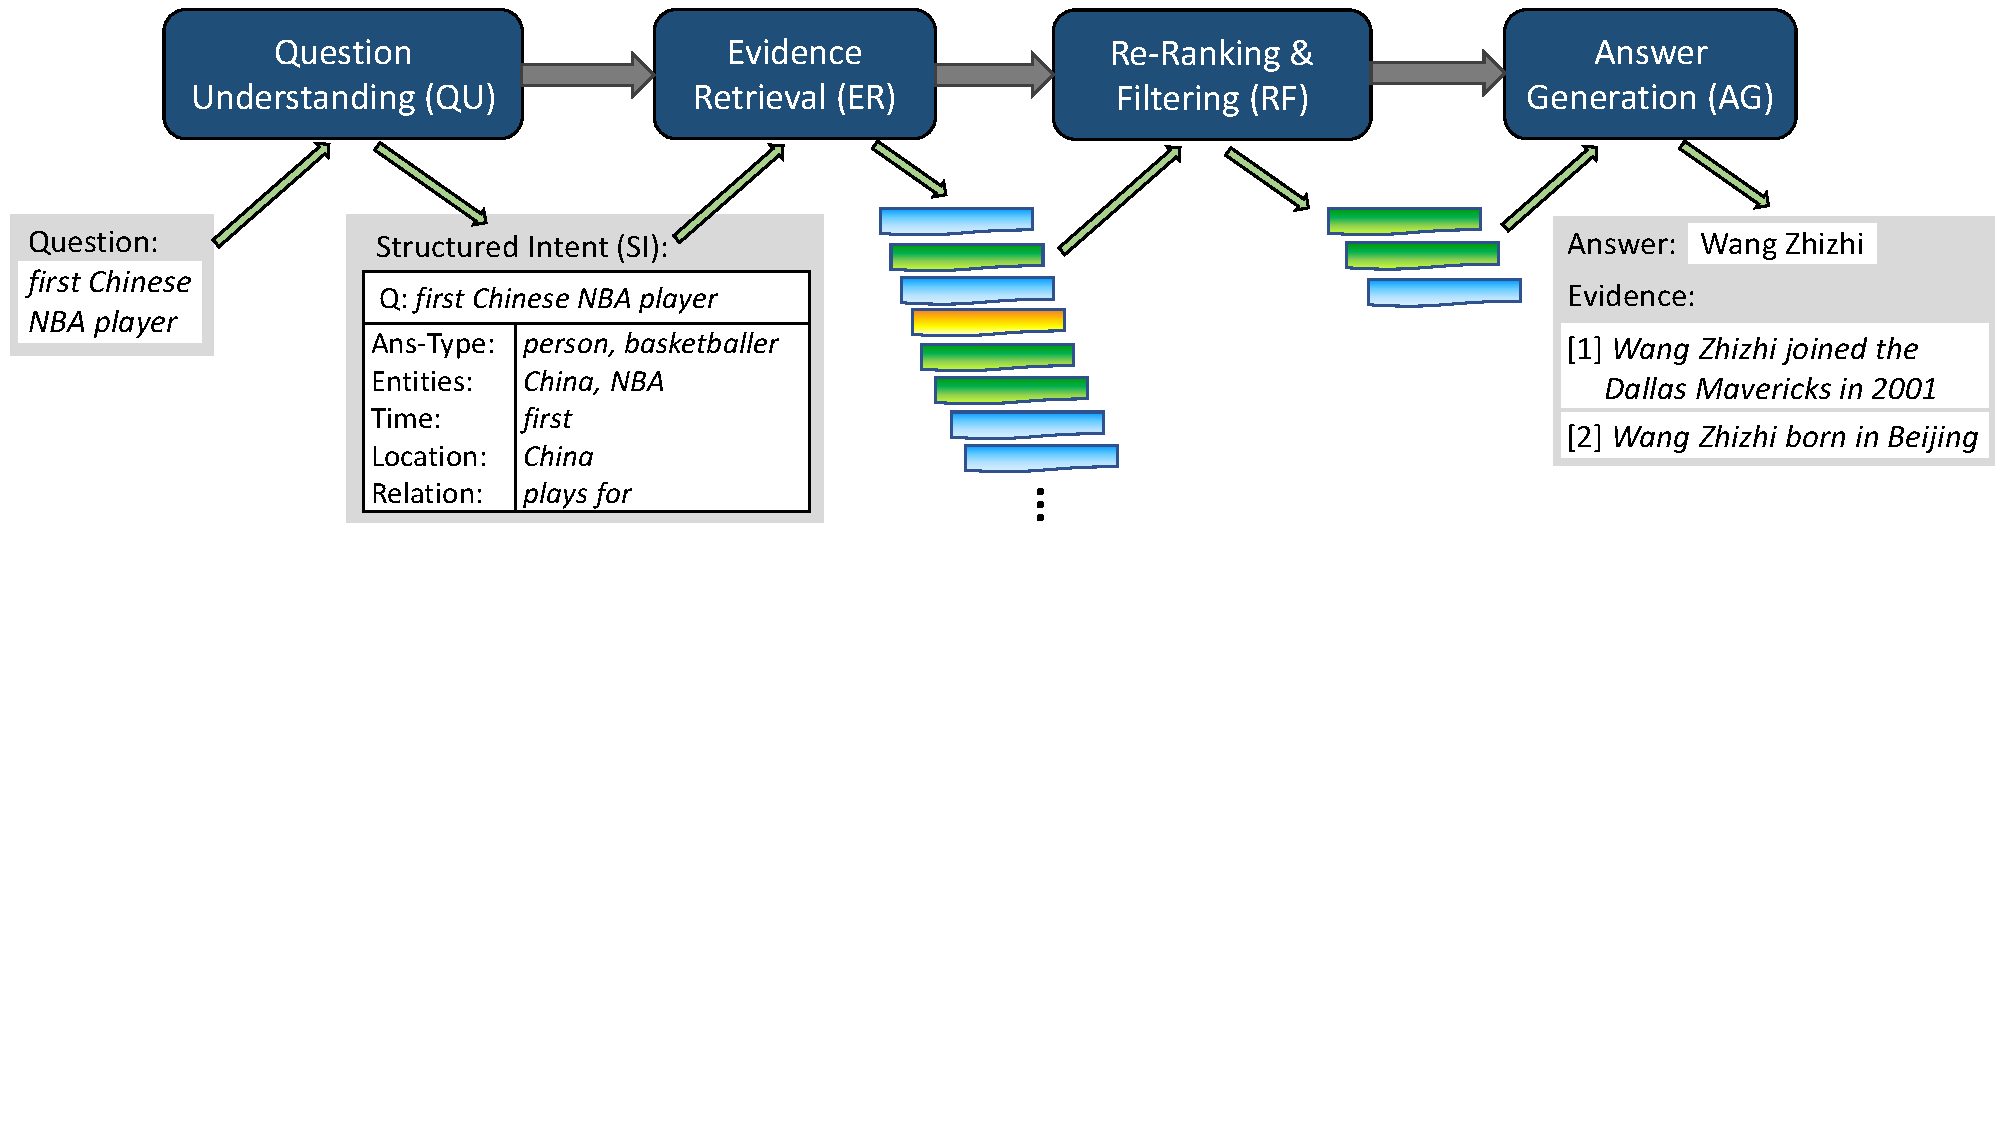
\includegraphics[width=\textwidth]{submissions/Gerhard2024/figures/compass-overview.pdf}
  \caption{Overview of the \method system.}
  \label{fig:compass-overview}
\end{figure}

% start with system overview
The \method system is a pipeline of four major stages, as illustrated in Figure \ref{fig:compass-overview}.
First, the input question is analyzed and decomposed, in order to compute a {\em structured intent (SI)} representation that will pass on to the subsequent steps, along with the original question. Second, the SI is utilized to retrieve pieces of evidence from different sources: text, KG and tables. 
Third, this pool of potentially useful evidence is filtered down, with iterative re-ranking, to arrive at a tractably small set of most promising evidence.
The final stage generates the answer from this evidence,
passing back the answer as well as evidence snippets for user-comprehensible explanation.

The second and fourth stage, Evidence Retrieval (ER) and Answer Generation (AG), are fairly standard. Such a two-phase architecture was called a retriever-reader architecture~\cite{Zhu-ODQA-survey:arxiv2021}. With a modern LLM replacing the earlier kinds of neural readers, this is the core of every RAG system~\cite{DBLP:journals/arXiv/abs-2312-10997}.

Stages 1 and 3 are unique elements of our architecture, judiciously introduced to improve both effectiveness (i.e., answer quality) and efficiency (i.e., computational cost).
Question Understanding (QU) provides the ER component with crisper and semantically refined input, and
the Re-Ranking \& Filtering (RF) stage is beneficial for
distilling the best evidence from the large pool of retrieved pieces.
The following subsections elaborate on the four stages of the pipeline, emphasizing the \method-specific steps QU and RF.



\subsection{Question Understanding (QU)}

% one par introducing the SI
To prepare the retrieval from different kinds of sources, including a KG, ad-hoc tables and text documents, it is useful to analyze and decompose the user question.
In this work, we aim to cast a question into a 
{\em structured intent (SI)} representation: essentially
a frame with faceted cues as slots, or equivalently, a concise set of key-value pairs. 
Figure \ref{fig:compass-overview} gives an idealized example for the question about the first Chinese NBA player. The facets or keys of potential interest here 
are:
\squishlist
\item {\em Ans-Type:} the expected answer type (or types when considering
different levels of semantic refinement), 
\item {\em Entities:} the salient entities in the question, and 
\item {\em Relation:} phrases that indicate which relation (between Q and A entities) the user is interested in. 
\squishend
\noindent In addition, as questions can have temporal or spatial aspects, the SI also foresees slots for:
\squishlist
\item {\em Time:} cues about answer-relevant time points or spans, including relative cues (e.g., ``before Covid'') and ordinal cues (e.g., ``first''), and
\item {\em Location:} cues about answer-relevant geo-locations.
\squishend

% discuss the spectrum of different SIs
\vspace{0.2cm}
\noindent The ideal SI for example question Q2 would look like:

\begin{quote}
{\em Ans-Type:} person, basketballer; {\em Entities:} China, NBA; {\em Time:} first;
{\em Location:} China; {\em Relation:} plays for.
\end{quote}

Note that the values for these slots can be crisp like entity names or dates, but they can also take the form of surface phrases. The SI purpose and value lie in the decomposition. In practice, many questions would only lead to a subset of faceted cues, leaving some slots empty. For the example in Figure \ref{fig:compass-overview}, an alternative SI could simply consist of

\begin{quote}
{\em Ans-Type:} person; {\em Entities:} China, NBA; {\em Time:} first.
\end{quote}

\noindent Even this simplified SI can be highly beneficial in guiding the subsequent evidence retrieval.

% sketch how an LM is trained to generate SIs 
To generate the SI from a user question, we employ a (small-scale) LM, specifically BART~\cite{DBLP:conf/acl/LewisLGGMLSZ20}, a Transformer-based auto-encoder with 140M parameters.\footnote{\url{https://huggingface.co/facebook/bart-base}}
BART is pre-trained for language representation; its power for our purpose comes from fine-tuning.
To this end, we generate (question, SI) pairs by using an instruction-trained LLM like GPT-4, with few-shot in-context learning (following our earlier work~\cite{Jia-FAITH:WWW2024}). 
Note that this is a one-time action; at inference-time we only use much smaller LMs.
The generated silver-standard pairs are then used to fine-tune BART.
In the experiments in this article, we leverage pre-existing collections of silver pairs, based on the training data of the CompMix benchmark~\cite{Christmann-CompMix:WWW2024}, 
comprising $3{,}400$ such pairs.


% outline value of SI for conversations
Although this paper focuses on single-shot questions, the \method architecture is also geared for conversational QA. In that setting, the SI can play an even bigger role, as (follow-up) questions are often formulated in a rather sloppy manner -- all but self-contained. For example, a conversation could start with a clear question {\em When did Wang Zhizhi join the NBA?}, followed a few dialog steps later, by a user utterance like {\em Which teams did he play for?} or simply {\em Which teams?}.
In such an informal conversation, the system needs to {\em contextualize} each user utterance based on the preceding turns in the dialog (e.g., inferring the relevant entities Wang Zhizhi and NBA from the conversational history).
For details on conversational QA, based on our architecture, see our earlier works~\cite{Christmann-CONVINSE:SIGIR2022,Christmann-Explaignn:SIGIR2023}.







%%%%%%%%%%%%%%%%%%%%%%%%%%%%%%%%%%%%%
\subsection{Evidence Retrieval (ER)}

The ER stage taps into a knowledge graph, a corpus of text documents, and a collection of web tables.
Specifically, for the experiments, we use the Wikidata KG,
all English Wikipedia articles, and all tables that are embedded in Wikipedia pages (incl. infoboxes, which can be seen as a special case of tables). 

% specifics: Clocq etc. - and the role of the SI
\vspace{0.2cm}
\noindent{\bf Retrieval from KG:}
To retrieve evidence from the KG, we utilize our earlier work
\clocq~\cite{Christmann-CLOCQ:WSDM2022}, which provides entity disambiguations and a relevant KG-subgraph for a given query.
Unlike most other works on QA-over-KG, \clocq fetches all KG-facts that are relevant for a given entity in a single step.
For example, when querying for
NBA players, it can traverse the KG neighborhood and pick up top teams, also considering so-called qualifier nodes in Wikidata which are often used for temporal scopes. 
As the disambiguation of entity names onto the KG can be tricky and noisy (e.g., China could be mapped to Chinese sports teams in all kinds of sports), \clocq considers several possible disambiguations~\cite{Christmann-CLOCQ:WSDM2022} (typically in the order of $10$ result entities).
The queries for \clocq are 
constructed by concatenating all slots of the question's SI.
For the example query about the first Chinese NBA player,
good result entities would be Dallas Mavericks, lists about NBA seasons, MVP awards etc., and their associated facts. These provide cues, but are likely insufficient to answer the question.


\vspace{0.2cm}
\noindent{\bf Retrieval from Text and Tables:}
The disambiguated entities returned by \clocq form anchors for tapping into text and tables.
\method first identifies 
relevant text documents and tables that refer to the anchor entities. With focus on Wikipedia, these are simply the articles for the respective entities. 
\method then constructs a keyword query that concatenates all available fields of the SI.
The query is evaluated against a linearized and verbalized representation (see below) of all sentences and all table rows in the selected documents.
This returns a set of sentences and 
and individual table rows, ranked by BM25 scores.


\vspace{0.2cm}
\noindent{\bf Evidence Verbalization:}
All results from the different data sources are uniformly treated by {\em linearizing} and {\em verbalizing} them
into token sequences. For KG results, the entity-centric triple sets are linearized via breadth-first traversal of the mini-graph starting from the entity node.
For tables, results are individual rows, which are contextualized by including labels from column headers and from the DOM-tree path of the article where the table comes from. For example, a table row about Wang Zhizhi playing for Dallas (Mavericks) in the 2000-2001 season, would be expressed as:

\vspace{0.05cm}
\hspace*{0.5cm} Wang Zhizhi / NBA Career / Season: 2000-2001, Team: Dallas, Games Played: 5 \dots
\vspace{0.05cm}

\noindent Finally, results from the text corpus are already in the form of token sequences, but we can additionally prefix these with the DOM-tree labels.
We can think of this entire pool of evidence as 
an on-the-fly corpus of potentially relevant pseudo-sentences, forming the input of the subsequent RF stage.


\vspace{0.2cm}
\noindent {\bf Result Ranking:}
Overall, the ER stage compiles a substantial set of evidence, possibly many thousands of entities, text snippets and table rows. Therefore, we practically restrict the pool to a subset of high-scoring pieces, like the top-$1000$.
For scoring, a simple BM25 model (a classical IR method) is applied. 
By default, we treat all evidence pieces uniformly with global scoring, no matter whether they come from KG, text or tables. 


\subsection{Re-Ranking and Filtering (RF)}

With a pool of top-$1000$ evidence pieces, we could invoke an LLM for answer generation. However, that would face a large fraction of noise (i.e., misleading evidence) and incur high costs of computation and energy consumption. 

For both of these reasons, we have devised light-weight techniques for iteratively reducing the top-$1000$ pieces to a small subset, say top-$30$ or top-$10$, that can be fed into an LLM at much lower cost (as LLM computations and pricing are at least linear in the number of input tokens). The difficulty is, of course, to do this without losing good evidence and reducing answer presence. Our techniques for this task are based on graph neural networks (GNNs)~\cite{Wu:IEEE2021} or cross-encoders (CEs)~\cite{Dejean:arxiv2024,Lin:MC2021}.

\myparagraph{GNN-based RF}
Given a large pool of evidence pieces from all sources, a bipartite graph is constructed:
\squishlist
\item {\em nodes} being evidence pieces or entities that occur in these pieces, and
\item {\em edges} connecting an evidence piece and an entity if the entity occurs in the evidence.
\squishend


The task for the GNN is to jointly score the evidence and the entity nodes in a multi-task learning setup. The latter are the {\em answer candidates}, and the evidence should give {\em faithful explanation} for an answer.
We build on our earlier work on explainable QA~\cite{Christmann-Explaignn:SIGIR2023}.

The node encodings are initialized with cross-encoder embeddings (see below) 
for node contents and the SI of the question. The inference iteratively adjusts the encodings based on message passing from neighboring nodes.
The GNN is trained via weak supervision from question-answer pairs:
evidence nodes are labeled as relevant if they are connected to
a gold answer.
More technical details are given in~\cite{Christmann-Explaignn:SIGIR2023}.

\method invokes the GNN in multiple rounds, iteratively reducing top-$k$ to top-$k^*$ nodes with $k^* \ll k$. In practice, we would typically consider two rounds: re-ranking top-$1000$ and pruning to top-100, and then reducing to top-30 or top-10, which are passed to the answer generation stage.
Note that this keeps the GNN at a tightly controlled size, so that its computational costs at inference-time are much smaller than those of an LLM.


\myparagraph{CE-based RF}
An alternative to the GNN inference is to employ a cross-encoder for scoring and re-ranking the evidence pieces.
These are transformers (typically with a small LM like BERT) that are fine-tuned for scoring the relatedness between a query and a document~\cite{Nogueira:arxiv2019}. In our case, the comparison is between the question SI and the evidence piece. In our experiments, we make use of two different cross-encoders, 
both trained on the MS-MARCO benchmark for passage retrieval~\cite{Bajaj:arxiv2018}, 
and fine-tuned on the respective benchmark (leveraging the same weak supervision data as for the GNNs),
the difference being in model size.\footnote{\url{https://huggingface.co/cross-encoder/ms-marco-MiniLM-L-4-v2} and\\ \url{https://huggingface.co/cross-encoder/ms-marco-MiniLM-L-6-v2}}
We use the smaller model to reduce top-$1000$ to top-100, and the larger model to go further down from top-100 to top-30.




%%%%%%%%%%%%%%%%%%%%%%%%%%%%%%%%%%%%%

\subsection{Answer Generation (AG)}

The last stage follows mainstream practice to invoke an LLM in a retrieval-augmented manner.
We call a `small-scale` LLM, specifically a fine-tuned LlaMA-3.1 model (8B-Instruct)\footnote{\url{https://huggingface.co/meta-llama/Llama-3.1-8B-Instruct}}, with a prompt \footnote{The specific prompt is \phrase{SI: \textless\texttt{concatenated SI}\textgreater \hspace{0.1cm} Evidence: \textless\texttt{evidence pieces}\textgreater}.}
consisting of:

\squishlist
\item the concatenated SI of the original question, and
\item the top-30 (or other top-$k^*$ with small $k^*$) evidence pieces.
\squishend

By the previous down-filtering of the original pool of evidence pieces, this last step has affordable cost in terms of computation time and energy consumption.

\vspace{0.2cm}
\noindent{\bf Fine-Tuning the LLM:}
We considered adding an instruction to the prompting, such as {\em ``answer this question solely based on the provided evidence snippets''}.
However, this turned out to be ineffective.
The reason why the model works well without such instructions is our task-specific fine-tuning.
We perform this by running the training data of benchmarks through the \method pipeline,
and training the AG stage with the top-30 evidence pieces as input.
Thus, the fine-tuning makes the model learn the role of evidence for RAG-based QA.

\vspace{0.2cm}
\noindent{\bf Explanations:}
The top-30 evidence pieces can be used to provide users with explanation of answers.
Optionally, these could be reduced further for comprehensibility.
Alternatively, we can fine-tune the LLM to provide both answers and concise explanations.
Since we can infer which evidences in the input mention the annotated ground-truth answers,
our method could be fine-tuned to provide such \textit{answering evidences} as well (cf.~\cite{Gao-citations:emnlp2023}).

\label{sec:exp}
\section{Experiments}


\label{setup}
\subsection{Experimental setup}


%%% BENCHMARKS
\myparagraphnospace{Benchmarks} We run experiments on three benchmarks with different characteristics of questions.

\squishlist
    \item \textbf{\compmix}.
    \compmix~\cite{Christmann-CompMix:WWW2024} is a benchmark which was specifically designed for evaluating QA systems operating over heterogeneous sources. The dataset has $9{,}410$ questions, out of which $2{,}764$ are used for testing.
    Answers are crisp entity names, dates, or other literals.
    
    \item \textbf{\crag}.
    We further evaluate on a subset of the \crag~\cite{Yang-CRAG} dataset, which was recently released as a testbed for RAG-based QA systems.
    We utilize the same pipeline and sources as outlined in Section~\ref{sec:method}, without using the web snippets or APIs provided with \crag. This way we focus on entity-centric questions that do not require access to live web data (e.g., news feeds), and disregard cases where the results would be up-to-date quantities.
    This restricts the test data to $436$ entity-centric questions, still enough for a proof of concept.
    
    \item \textbf{\timequestions}.
    To showcase the generalizability of our pipeline, we conduct experiments on~\timequestions~\cite{Jia-TimeQuestions},
    a benchmark for temporal QA. The dataset requires temporal understanding and reasoning, which are well-known limitations of
    LLMs~\cite{Dhingra-time-aware-LLM:TACL2022}. \timequestions has 16{,}181 questions (3{,}237 for testing).
\squishend

Typical examples for the questions in these three benchmarks are:

\begin{quote}
\compmix: \utterance{Which player won the most number of Man-of-the-Match titles in the FIFA world cup of 2006?}\\
 \indent \crag: \utterance{What was the worldwide box office sales for little hercules?}\\ 
  \indent \timequestions: \utterance{Which club did Cristiano Ronaldo play for before joining Real Madrid?}
\end{quote}

%%% BASELINES
\myparagraph{Baselines} As competitors or reference points to \method, we study the performance of the following methods:

\squishlist
    \item \textbf{Generative LLMs}.
    We compare \method against out-of-the-box LLMs: \textbf{\gptthree} (\texttt{text-davinci-003}), \textbf{\gptfour} (\texttt{gpt-4}) 
    and \textbf{\llama} (\texttt{meta-llama/Llama-3.1-8B-Instruct}).
    The same prompt is used for all LLMs, consistent with previous work~\cite{Christmann-CompMix:WWW2024, Zhang-Spaghetti:ACL2024}:
    \phrase{Please answer the following question by providing the crisp answer entity, date, year, or numeric number. Q: \textless\texttt{question}\textgreater}.
    

    \item \textbf{Heterogeneous QA methods}.
    \convinse~\cite{Christmann-CONVINSE:SIGIR2022}, \unikqa~\cite{Oguz-UniK-QA:NAACL2022}, \explaignn~\cite{Christmann-Explaignn:SIGIR2023}
    are QA methods designed to integrate heterogeneous sources: text, tables and KG. All of these  integrate the exact same sources as \method.

    
    \item \textbf{\textsc{State-of-the-art}}.
    For \compmix and \timequestions, we also compare against state-of-the-art methods from the literature: \spaghetti~\cite{Zhang-Spaghetti:ACL2024} and \textsc{Un-Faith}~\cite{Jia-FAITH:WWW2024}, which are among the best performing systems.
    
Results are taken from the literature whenever applicable.
On \crag, we use the models trained on \compmix for \method and heterogeneous QA baselines.
\squishend



%%% METRIC(S)
\myparagraph{Metrics}
We measure \textit{precision at 1} (\textbf{P@1}) as our main metric~\cite{RoyAnand:MC2021} on all benchmarks.
On \crag, we manually annotate answer correctness, as the ground-truth answer formats vary (e.g., entity name variants, lists, sentences).

We also compute the number of neural parameters aggregated over all sub-modules (\textbf{\#Parameters}).
Parameter counts for GPT-models are taken from~\cite{Minaee-LLM-survey}
(\gptfour might have less active parameters during inference).

For further analysis we measure \textit{answer presence} (\textbf{AP@k}),
i.e. whether the answer is present in the top-$k$ ranked evidence pieces,
and \textit{mean reciprocal rank} within the top-$k$ evidences (\textbf{MRR@k}).

%%% CONFIG
\myparagraph{Configuration}
Our implementation uses the \texttt{Llama3.1-8B-Instruct} model for the AG stage.
For the QU, ER and RF stages
we adopt code from the \explaignn project.\footnote{\url{https://explaignn.mpi-inf.mpg.de}}
For the ER stage, we use \clocq, setting its specific parameters to $k=10$ and $p=1{,}000$.

As default, we use the GNN technique for the RF stage.
For efficiency, we use light-weight models for initializing
the GNN encoders -- the same models used for the CE-based RF.\footnote{\url{https://huggingface.co/cross-encoder/ms-marco-MiniLM-L-4-v2} and\\\url{https://huggingface.co/cross-encoder/ms-marco-MiniLM-L-6-v2}}
The GNNs are trained for $5$ epochs with an epoch-wise evaluation strategy,
i.e. we choose the model with the best performance on the respective dev set.
We train the GNNs on graphs with a maximum of $100$ evidence and $400$ entity nodes (as scored by BM25).
During inference, the first GNN is applied on graphs with $1{,}000$ evidence and $4{,}000$ entity nodes, shrinking the pool of evidence pieces to the top-$100$.
The second GNN then runs on graphs with $100$ evidence and $400$ entity nodes.
The factor of 4 entities per evidence (on average) holds sufficient for the observed data,
and enables batched inference.
Other parameters are kept as is.

The AG model, based on \texttt{Llama3.1-8B-Instruct}, is 
fine-tuned
for $2$ epochs with a warm-up ratio of $0.01$ and a batch size of $8$, again with an epoch-wise evaluation strategy.
Other parameters are set to the default Hugging Face
training parameters.\footnote{\url{https://huggingface.co/docs/transformers/v4.46.2/en/main_classes/trainer\#transformers.TrainingArguments}}





\subsection{Main results}
%%% MAIN TABLE
\myparagraphnospace{\method is competitive on all benchmarks}
Main results of our experiments are shown in Table~\ref{tab:main-res}.
First of all, we note that \method achieves competitive performance across all three benchmarks.

On \compmix, baselines for heterogeneous QA and \llama perform similarly,
whereas GPT-based LLMs can answer more than $50$\% of the questions correctly.
\method exhibits substantially higher performance, on par with
the state-of-the-art method \textsc{Spaghetti}~\cite{Zhang-Spaghetti:ACL2024}
(which is based on \gptfour).

On the \crag dataset, P@1 drops for all methods except for \gptfour. 
The benchmark includes realistic questions,
which can be ambiguous/confusing (\phrase{who was the director for the report?}),
on ``exotic'' entities with answers in social media (\phrase{how many members does the teknoist have?}),
or require up-to-date information (\phrase{when did chris brown release a song or album the last time?}),
and other cases that are challenging for all methods.

Finally, \method establishes new state-of-the-art performance on the \timequestions benchmark.
Interestingly, all of the tested LLMs show greatly reduced performance on this benchmark,
which inherently requires temporal understanding and reasoning
-- a known weakness of stand-alone LLMs.


\begin{table} [h]
    \centering
    \newcolumntype{G}{>{\columncolor [gray] {0.90}}c}
    \begin{tabular}{l G G G c}
        \toprule
            \textbf{Method $\downarrow$ / Benchmark $\rightarrow$} & \textbf{\compmix}  & \textbf{\crag} & \textbf{\timequestions} & \textbf{\#Parameters} \\ 
        \midrule
            \textbf{\gptthree} 
            & $0.502$ &   $-$ & $0.224$ & $175{,}000$ M  \\
            % #params from https://arxiv.org/pdf/2402.06196

            \textbf{\gptfour}
            & $0.528$ &   $\mathbf{0.633}$ & $0.306$ & $1{,}760{,}000$ M \\
            % #params from https://arxiv.org/pdf/2402.06196

            \textbf{\llama~\cite{Touvron-LLaMA}} (8B-Instruct)
            & $0.431$ &   $0.385$ & $0.178$ & $8{,}030$ M  \\
            % #params from Huggingface (8,030,257,152)
        \midrule
            \textbf{\convinse~\cite{Christmann-CONVINSE:SIGIR2022}}
            & $0.407$  &   $0.298$ & $0.423$  & $362$ M \\
            % FiD: 222,903,936 + BART (SR-generation): 139,420,416 = 362,324,352 (python explaignn/question_understanding/structured_representation/get_num_params.py)

            \textbf{\unikqa~\cite{Oguz-UniK-QA:NAACL2022}}
            & $0.440$ &   $0.280$ & $0.424$ & $223$ M  \\
            % FiD: 222,903,936 (python explaignn/heterogeneous_answering/fid_module/FiD/get_num_params.py)
    
            \textbf{\explaignn~\cite{Christmann-Explaignn:SIGIR2023}} 
            & $0.442$ &   $0.303$ & $0.525$  & $328$ M \\
            % BART (SR-generation): 139,420,416 + 2GNNs: 94520832 + 93930240 = 327,871,488

        \midrule 
            \textbf{\textsc{State-of-the-art}}
            & $\mathbf{0.565}$ 
            & $-$
            & $0.571$  & $-$ \\

            & (\textsc{Spaghetti}~\cite{Zhang-Spaghetti:ACL2024})
            & 
            & (\textsc{Un-Faith}~\cite{Jia-FAITH:WWW2024}) &  \\

        \midrule
            \textbf{\method (ours)}
            & ${0.564}$ &   $0.362$ & $\mathbf{0.754}$  & $8{,}218$ M \\
            % BART (SR-generation): 139,420,416 + LLaMA: 8,030,257,152 + GNNs: 25,670,016 + 22,268,928 =  8,217,616,510
        \bottomrule
    \end{tabular} 
    \vspace*{-0.2cm}
    \caption{End-to-end P@1 of \method and baselines on three benchmarks. Results for \gptthree and \gptfour are taken from the literature~\cite{Christmann-CompMix:WWW2024, Jia-FAITH:WWW2024}. \gptthree is not accessible anymore, hence no results on \crag.
    }
    \label{tab:main-res}
\end{table}





%%% ANSWER SOURCES
\myparagraph{Integration of heterogeneous sources is vital}
\method integrates evidence from text, KG and tables into a unified framework.
We aim to better understand how this affects the answering performance of the method.
Table~\ref{tab:sources} shows end-to-end answering performance of \method
with different combinations of the input sources.
The results clearly indicate that all types of sources contribute, with option Text+KG+Tables performing best,
with a large margin over tapping only single source types.

\begin{table} [t] 
    \centering
    \newcolumntype{G}{>{\columncolor [gray] {0.90}}c}
    \newcolumntype{H}{>{\setbox0=\hbox\bgroup}c<{\egroup}@{}}
    	\begin{tabular}{l G G G H H H c c c} 
        \toprule
            \textbf{Benchmark $\rightarrow$}
                & \multicolumn{3}{G}{\textbf{\compmix}} 
                & \multicolumn{3}{H}{\textbf{\crag}}
                & \multicolumn{3}{c}{\textbf{\timequestions}} \\ 
        \midrule
            \textbf{Input sources $\downarrow$ / Metric $\rightarrow$}
                & \textbf{P@1} & \textbf{AP@100}  & \textbf{AP@30}
                & \textbf{P@1} & \textbf{AP@100}  & \textbf{AP@30}
                & \textbf{P@1} & \textbf{AP@100}  & \textbf{AP@30} \\
            \midrule
                \textbf{Text}           &  $0.455$  &  $0.563$  &  $0.531$ &  $?$  &  $?$  &  $?$ &  $0.539$  &  $0.515$  &  $0.487$   \\
                \textbf{KG}             &  $0.481$  &  $0.677$  &  $0.637$ &  $?$  &  $?$  &  $?$ &  $0.724$  &  $0.701$  &  $0.674$   \\
                \textbf{Tables}         &  $0.432$  &  $0.501$  &  $0.482$ &  $?$  &  $?$  &  $?$ &  $0.536$  &  $0.347$  &  $0.328$   \\
            \midrule
                \textbf{Text+KG}        &  $0.537$  &  $0.749$  &  $0.706$ &  $?$  &  $?$  &  $?$ &  $0.745$  &  $\mathbf{0.776}$  &  $0.748$   \\
                \textbf{Text+Tables}    &  $0.503$  &  $0.632$  &  $0.594$ &  $?$  &  $?$  &  $?$ &  $0.567$  &  $0.578$  &  $0.549$   \\
                \textbf{KG+Tables}      &  $0.524$  &  $0.728$  &  $0.692$ &  $?$  &  $?$  &  $?$ &  $ 0.743$  &  $0.731$  &  $0.703$   \\
            \midrule
                \textbf{Text+KG+Tables}    &  $\mathbf{0.564}$  &  $\mathbf{0.759}$  &  $\mathbf{0.724}$ &  $?$ &  $?$  &  $?$ & $\mathbf{0.754}$    & $\mathbf{0.776}$  &  $\mathbf{0.749}$   \\
            \bottomrule
    \end{tabular}
    \vspace*{-0.2cm}
    \caption{Answer presence and answering precision of \method with different combinations of input sources (on the respective test sets).}
    \label{tab:sources}
\end{table}




\subsection{Analysis}

%%% TOP-K vs. 3xTOP-(K/3)
\myparagraph{Unified retrieval enhances performance}
In the RF stage, we re-rank and filter evidence from different source types,
and feed the unified top-\textit{k}* into the AG stage.
We conduct a comparison in which we consider
the top-$10$ evidence pieces from each source type individually. This gives equal influence to KG, text and tables, whereas our default is based on global ranking.
Table~\ref{tab:unified-retrieval} shows the results for this analysis, showing our default choice performs better.
The reason is that different questions require different amounts of evidence from each of the source types.

\begin{table} [t] 
    \centering
    \newcolumntype{G}{>{\columncolor [gray] {0.90}}c}
    \newcolumntype{H}{>{\setbox0=\hbox\bgroup}c<{\egroup}@{}}
    	\begin{tabular}{l G G H H} 
        \toprule
            \textbf{Input evidences $\downarrow$ / Metric $\rightarrow$} & \textbf{P@1} & \textbf{AP@30}  & \textbf{\crag} & \textbf{\timequestions} \\ 
            \midrule
                \textbf{Top-30 Text+KG+Tables (ours)}             &  $\mathbf{0.574}$  &  $\mathbf{0.710}$  &  $-$  &  $-$   \\
                \textbf{Top-10 Text + Top-10 KG + Top-10 Tables}        &  $0.560$    &  $0.709$  &  $-$  &  $-$   \\
            \bottomrule
    \end{tabular}
    \vspace*{-0.2cm}
    \caption{Answer presence and precision
    of \method for different choices of top-30 
    (on \compmix dev set).}
    \label{tab:unified-retrieval}
\end{table}


%%% NUMBER OF EVIDENCES
\myparagraph{\method works well with small amounts of evidence}
We investigate the 
influence of 
the number of evidence pieces
fed into the AG stage, varying it from $5$ to $100$.
Results are shown in Figure~\ref{fig:res-num-evidences}.
As the curve shows, there is a sharp increase in precision as we add evidence up to 30 or 40 pieces, which is around our default of top-30. This indicates that a certain amount of evidence is needed, to overcome the inherent noise and arrive at sufficient answer presence. 
As we increase the amount of evidence further, we observe a saturation effect, and eventually a degration of performance. Too much evidence not only has diminishing returns, but can actually be confusing for the AG stage. This reconfirms our heuristic choice of top-30: enough for good answering while keeping computational costs reasonably low.


\begin{figure}[t]
    \centering
    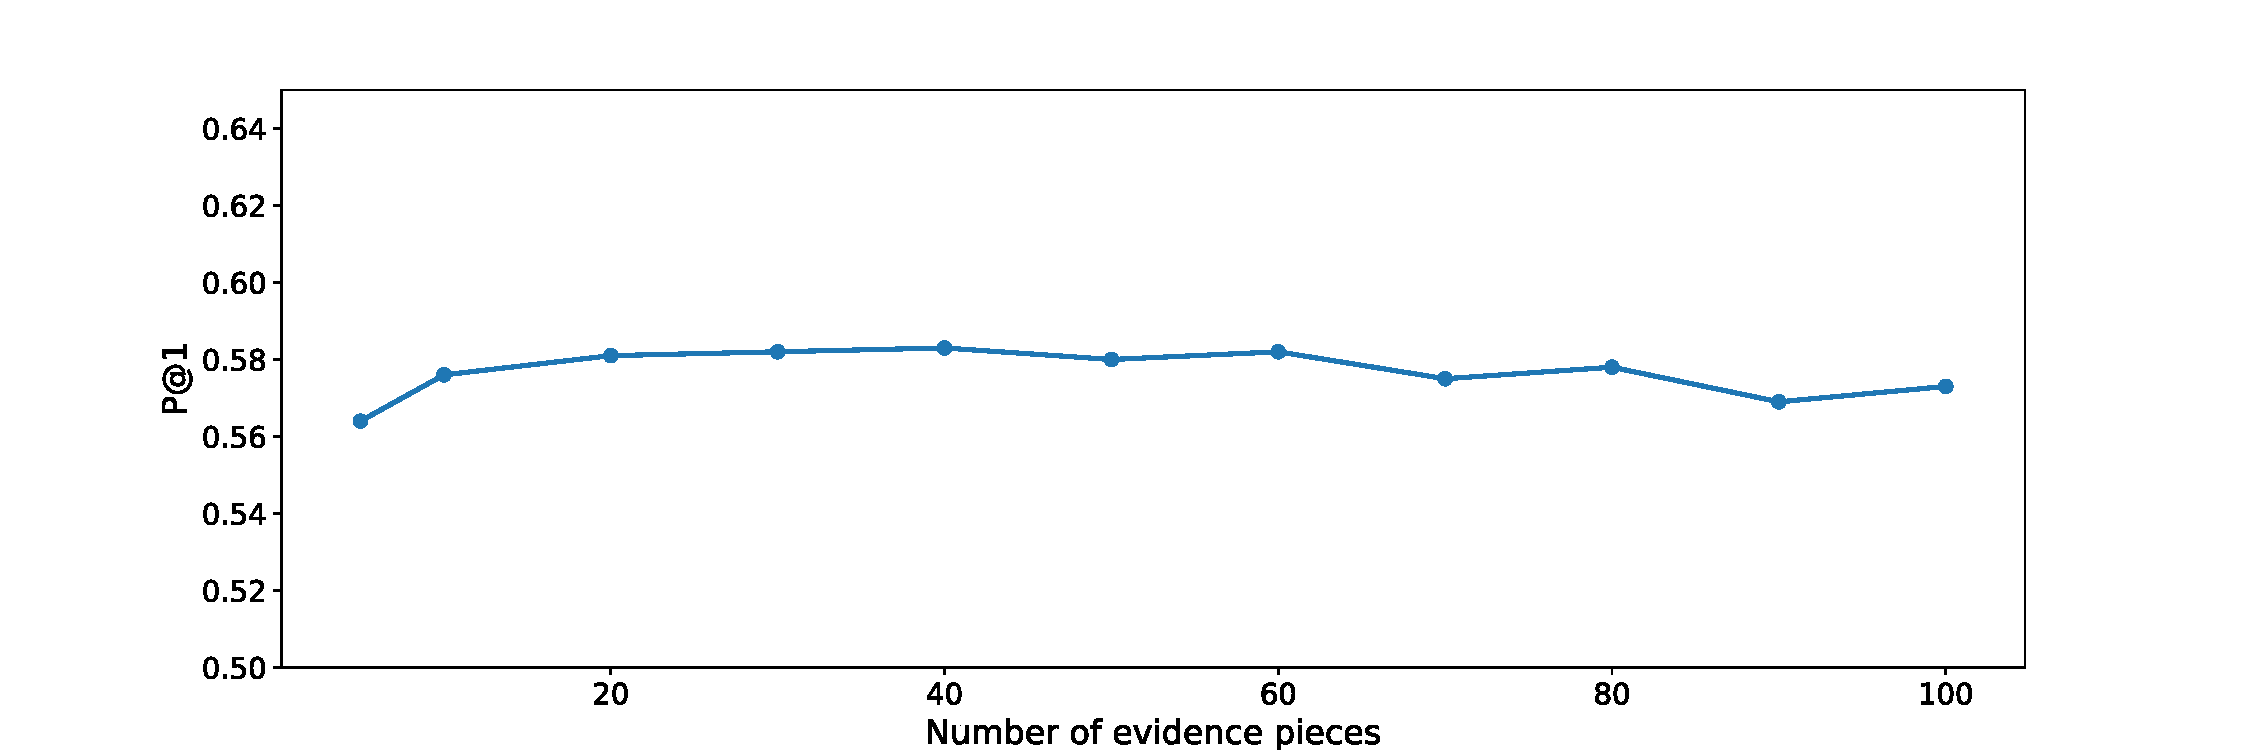
\includegraphics[width=0.8\textwidth]{submissions/Gerhard2024/figures/p_at_1-line_with_evidences.pdf}
    \vspace*{-0.2cm}
    \caption{Performance of \method on the \compmix dev set with different numbers of evidence.}
    \label{fig:res-num-evidences}
    \vspace*{-0.2cm}
\end{figure}



%%% ABLATION
\myparagraph{Ablation study on re-ranking} For more insight on the possible configurations of the RF stage, we conducted an ablation study with different options, including solely relying on the initial BM25 scoring without explicit re-ranking. The results are shown in Table \ref{tab:ablation2}. We observe that the iterative reduction in two steps is slightly better than the single-step variants (going down from top-1000 to top-30 in one RF step). Between the two options of using a GNN or a CE, the differences are negligible. A notable effect is that our RF techniques retain the answer presence at a very high level, only a bit lower than for the initial top-1000. 
The last two rows of Table \ref{tab:ablation2} demonstrate that RF is crucial: without explicit re-ranking, the technique of just picking smaller top-$k$ from the original BM25 model leads to substantial degradation in both answer presence and precision. 


\begin{table} [t] \small
    \centering
    \newcolumntype{G}{>{\columncolor [gray] {0.90}}c}
    \newcolumntype{H}{>{\setbox0=\hbox\bgroup}c<{\egroup}@{}}
    	\begin{tabular}{l G H G G G} 
        \toprule
            & \multicolumn{5}{G}{\textbf{\compmix} (dev set)} \\
        \midrule
            \textbf{RF Method $\downarrow$ / Metric $\rightarrow$} & \textbf{P@1} & \textbf{AP@1000} & \textbf{AP@100}  & \textbf{AP@30} & \textbf{MRR@100} \\ 
        \midrule
            \textbf{GNN: 1000 $\rightarrow$ 100 $\rightarrow$ 30}             &  $\mathbf{0.574}$  & $0.760$ &  $0.738$  &  $0.710$  &  $\mathbf{0.572}$  \\
            \textbf{CE: 1000 $\rightarrow$ 100 $\rightarrow$ 30}          &  $0.573$  & $0.760$  &   $\mathbf{0.740}$ &  $\mathbf{0.721}$   &  $0.553$   \\
        \midrule
            \textbf{GNN: 1000 $\rightarrow$ 30} &  $0.567$  & $?$  &   $n/a$ &  $0.710$   &  $0.567$   \\
         \textbf{CE: 1000 $\rightarrow$ 30} &  $0.570$  & $0.760$  &   $n/a$ &  $0.715$   &  $0.558$   \\
            \midrule
           \textbf{BM25: 100 (w/o GNN or CE)} &  $0.490$ & $0.760$  &  $0.652$  &  $n/a$  &  $0.259$ \\       
            \textbf{BM25: 30 (w/o GNN or CE)} &  $0.468$  & $0.760$  &  $n/a$ &  $0.534$   &  $0.259$   \\
            \bottomrule
    \end{tabular}
    \vspace*{-0.2cm}
    \caption{Ablation study for different RF strategies of \method on the \compmix dev set. The answer presence in the RF input with top-$1000$ evidence pieces is $0.760$.}
    \label{tab:ablation2}
\end{table}



\myparagraph{Quality of SI}
To assess the quality and robustness of the Structured Intents, we
inspected a sample of questions and their SIs.
Table~\ref{tab:question-SI-examples} gives three anecdotic examples.
We show SIs generated by \method, which makes use of the pre-existing collection from the \compmix benchmark for training.
This training data was obtained via different heuristics, 
which can be a limiting factor when user intents become more complex.

Therefore, we also looked at SIs derived via in-context learning (ICL) using \gptfour with $5$ handcrafted examples.
As shown in our earlier work on temporal QA~\cite{Jia-FAITH:WWW2024},
such data can be used for training smaller models (e.g., BART),
which can greatly boost the completeness and overall quality of the generated SIs.

From the sampled set, we observed that the ICL-based SIs are more
complete with all slots filled, whereas the BART-based SIs focused more
on the main slots Answer-type, Entities and Relation.
However, both approaches achieve very high quality in filling the slots,
capturing the user's information need very well.

Interestingly, when questions get complicated, with nested phrases, 
the ICL-based variant succeeds in decomposing the questions, based on only $5$ ICL examples.
For example, for the question {\em ``which German state had the most Corona-related death cases in the first year after the outbreak?''}
the Time slot becomes {\em ``first year after Corona outbreak''},
which can be resolved to identify the temporal scope.
In general, we believe that such question decomposition, beyond simple temporal constraints,
would be an interesting theme for future work.

\begin{table} [t] 
    \centering
    \small
    \newcolumntype{G}{>{\columncolor [gray] {0.90}}c}
    \newcolumntype{H}{>{\setbox0=\hbox\bgroup}c<{\egroup}@{}}
    \resizebox*{\textwidth}{!}{
        \begin{tabular}{p{6cm}|p{6cm}|p{6cm}} 
        \toprule
            \textbf{Question} & \textbf{Current SI by \method} & \textbf{SI via ICL} \\
        \midrule
        \textit{what was disneys first color movie?}
            & Ans-Type: \textit{animated feature film} & Ans-Type: \textit{film, animated film} \\
            & Entities: \textit{disneys} & Entities: \textit{Disney} \\
            & Relation: \textit{was first color movie} & Relation: \textit{first color movie} \\
            &  & Time: \textit{first} \\
        \midrule
        \textit{at the oscars, who won best actor in 2018?}
            & Ans-Type: \textit{human} & Ans-Type: \textit{person, actor} \\
            & Entities: \textit{at the oscars} & Entities: \textit{Oscars, 2018} \\
            & Relation: \textit{who won best actor in 2018} & Relation: \textit{won best actor} \\
            &  & Time: \textit{2018} \\
        \midrule
        \textit{which German state had the most Corona-} & Ans-Type: \textit{state} & Ans-Type: \textit{location, state} \\
        \textit{related death cases in the first year after} & Entities: \textit{Germany, Corona} & Entities: \textit{Germany, Corona-related deaths} \\
        \textit{the outbreak?} & Relation: \textit{which state had the most related} & Relation: \textit{highest count of death cases} \\
        & \textit{death cases in the first year after the out-}  & Location: \textit{Germany} \\
            & \textit{break}  & Time: \textit{first year after Corona outbreak} \\
        \bottomrule
    \end{tabular}
    }
    \vspace*{-0.2cm}
    \caption{Examples for pairs of question and generated SI.}
    \label{tab:question-SI-examples}
\end{table}




%%% REFRAIN FROM ANSWER
\myparagraph{Refraining from answering}
%%% Searched for: "generated_answer I" (with I being the full word, not partial) in the generated answers of LLaMA
%%% yields 245 results out of 2764 questions on CompMix
%%% yields 1270 results out of 3237 questions on TimeQuestions
We can train our model to refrain from answering in scenarios
where the provided evidence does not contain an answer to the question.
Specifically, during training, when the answer is not present in the evidence,
we change the target answer to {\em unknown}. This variant is referred to as \method {\em (faithful)}.

We measure the ratio of questions for which {\em unknown} is provided as answer,
and the P@1 restricted to questions that are answered.
The accuracy of refraining from answering is measured as well,
based on whether the answer is present in the evidence or not.
We conduct this experiment on \compmix and \timequestions,
for which we can compute answer presence exactly.
We also compute results for \llama, which is already instructed 
with the option to answer ``don't know''.
Table~\ref{tab:refrain-from-answer} shows the results.
For \compmix, we observe that \method has high accuracy on refraining when appropriate,
whereas \llama tends to be overconfident with a very small rate of {\em unknowns}, leading to incorrect answers.

\begin{table} [t] \small
    \centering
    \newcolumntype{G}{>{\columncolor [gray] {0.90}}c}
    \newcolumntype{H}{>{\setbox0=\hbox\bgroup}c<{\egroup}@{}}
    	\begin{tabular}{l G G G G c c c c} 
        \toprule
            & \multicolumn{4}{G}{\textbf{\compmix}} & \multicolumn{4}{c}{\textbf{\timequestions}} \\
            \midrule
            \textbf{Metric $\rightarrow$} & \textbf{P@1}  & \textbf{P@1} & \textbf{Refrain} & \textbf{Refrain} & \textbf{P@1}  & \textbf{P@1} & \textbf{Refrain} & \textbf{Refrain} \\ 
            \textbf{Method $\downarrow$} &                 & \textbf{(answered)} & \textbf{rate} & \textbf{accuracy} &                 & \textbf{(answered)} & \textbf{rate} & \textbf{accuracy} \\ 
            \midrule
                \textbf{\llama}             &  $0.431$  &  $0.471$  &  $0.089$  &  $n/a$  &  $0.177$  &  $0.276$  &  $0.392$  &  $n/a$  \\
                \textbf{\method (faithful)}           &  $0.497$  &  $0.713$  &  $0.303$  &  $0.838$ &  $0.597$  &  $0.804$  &  $0.257$  &  $0.864$  \\
            \bottomrule
    \end{tabular}
    \vspace*{-0.2cm}
    \caption{
        Performance of \method with option to refrain from answering (``don't know'').
    }
    \label{tab:refrain-from-answer}
\end{table}

\label{sec:disc}
\section{Insights, Limitations, and Challenges}


\noindent{\bf Benchmark Performance.} Our method, RAG-based \method with an 8B LLaMA model, outperforms much larger LLMs like \gptfour on two of the three benchmarks, with a very large margin for temporal questions. Obviously, pre-trained LLMs have only limited sense of properly positioning ``remembered’’ facts on the timeline even with training data that exceeds ours by several orders of magnitude. This confirms our intuition that LLMs alone are not good at ``recalling’’  higher-arity relations that require combining distant pieces of evidence. This is a sweet spot for RAG. Only for 
the \crag benchmark, \method is substantially inferior to a full-blown LLM. This is likely due to the nature of the questions: not necessarily the complexity of the information needs, but the need for more web sources (beyond what our experiments tap into).

\vspace{0.2cm}
\noindent{\bf Cost/Performance Ratio.} The most important take-away from our experiments is that \method achieves its competitive performance at a much lower cost than the full LLMs. Assuming that the consumed GFlops are proportional to the number of model parameters, \method achieves a cost reduction by a factor of 200x for \gptthree and 2000x for \gptfour. This does not only mean less computation, but also a massively lower electricity bill and climate impact.  

\vspace{0.2cm}
\noindent{\bf Role of Question Understanding.} We did not systematically investigate the influence of the Structured Intent in the \method pipeline. However, the comparison to the big GPT models reflects the role of the SI, as we prompt the GPT models in their natural mode with the original questions. The linearized sequence of available SI slots does not always have major advantages, but there are enough cases where specific facets provide crucial cues. This holds especially for the Entities slot, as this drives the gathering of evidence in the ER stage (cf.~\cite{Christmann-CONVINSE:SIGIR2022}, and for the Time slot, as these cues are often decisive for temporal questions (cf.~\cite{Jia-FAITH:WWW2024}).

\vspace{0.2cm}
\noindent{\bf Role of Re-Ranking.} As our ablation studies show, merely using top-$k$ evidence from an initial BM25-style ranking does not provide good performance. Also, there seems to be sweet spot in the choice of $k$: we need enough evidence for connecting the dots if the question requires multiple pieces of information, or for corroborating candidates if the question finds many useful but noisy pieces. In the experiments, $k=30$ turns out to be good choice; much lower $k$ results in insufficient evidence, and much larger $k$ leads to saturation and ultimately degrading performance. Our argument for iteratively shrinking the candidate set in multiple rounds of re-ranking is substantiated in our experiments, but the gain of doing this, compared to GNN- or CE-based re-ranking from 1000 to 30, is not big. More research is called to better understand the role of ranking in RAG. 

\vspace{0.2cm}
\noindent{\bf Limitations of Evidence Retrieval.}
For ER, we adopted more or less standard techniques. The results showed very good answer presence, in the order of 75\% in the top-100 or even top-30. An important case where this is insufficient are questions that require aggregating information over a large number of evidence pieces. An example is asking for the life-time total of 3-point scores of the basketball player Dirk Nowitzki.
This requires collecting a set of per-season tables with NBA player statistics, but also other web sources with numbers for his career before he joined the NBA (including his youth teams).
Of course, there are sometimes shortcuts like a Wikipedia article or biography mentioning the total number, but this cannot be universally assumed. The bottom line is that ER should be reconsidered as well, striving to improve the recall dimension.

\vspace{0.2cm}
\noindent{\bf Limitations of Answer Generation.}
For AG, we simply rely on a LLM,
using it as an extractor (``reader'') from the given evidence. Despite the wide belief that LLMs can perform deep
reasoning over many pieces of evidence, our experience is that the extraction works only well – robustly and faithfully – for relatively simple questions with a few multi-hop joins or simple aggregation over a few pieces. However, complicated questions such as asking for the top-100 NBA players with the largest number of life-time 3-point scores (again including their pre-NBA careers) are currently out of scope and will likely remain so for quite some time. This offers many opportunities for pushing the envelope further.

\vspace{0.2cm}
\noindent{\bf Trust in Data Sources.}
In our experiments, we considered all heterogeneous sources as trustworthy and unbiased. With focus on Wikidata and Wikipedia, this assumption has been well justified. In the wild, however, input data for RAG-based systems likely exhibit a wide spectrum of quality issues, in terms of stale information, biased positions, or simply false statements. Identifying trustworthy and up-to-date evidence and dealing with conflicting data, has been explored in other contexts (e.g., for KG curation~\cite{Dong-Trust:PVLDB2015}), but remains a major challenge for RAG-based QA.


\vspace{0.2cm}
\noindent{\bf Open Challenges and Future Work.} The best-performing methods in our experiment, mostly \method, reach P@1 values of 56\% for \compmix and 75\% for \timequestions. 
For the latter, the answer presence in the top-100 is only slightly higher; so the AG stage hardly misses anything.
However, for \compmix, the answer presence is 75\% -- much higher than what our system can actually answer. Obviously, closing this gap is a major direction to pursue, with focus on the RF and AG stages. However, missing one fourth of the answers completely in the top-100 pool, is a big problem as well. This requires improving recall at the ER stage, possibly with better guidance by the QU, which in turn needs more sources beyond the scope of our experiments (currently limited to Wikidata and Wikipedia). 

In general, we need to think beyond this kind of ``benchmark mindset’’. Even if we reached 80\% or 90\% precision and recall, we would still have a substantial fraction of questions that are answered incorrectly
or not at all. 
The remaining errors may not be a problem for chatbots, but they would be a showstopper for the deployment of mission-critical applications in business or science. We believe that this big gap is a shortcoming of {\em all methods}, not an issue that comes from the data alone. For trivia-style QA, as looked at in this paper, a smart human in ``open book’’ mode and no time limitation should be able to properly answer practically all questions, just by reading pieces of web contents and putting things together. Neither LLMs nor state-of-the-art RAG are the final solution; substantial research and creative ideas are needed to further advance QA.


\clearpage
\newpage

\newcommand{\bibauthors}[1]{{#1}}
\newcommand{\bibtitle}[1]{\emph{#1}}
\newcommand{\bibconf}[1]{{#1}}

\begin{thebibliography}{10}

\bibitem{Bajaj:arxiv2018}
\bibauthors{Payal Bajaj, Daniel Campos, Nick Craswell, Li Deng, Jianfeng Gao, Xiaodong Liu, Rangan Majumder, Andrew McNamara, Bhaskar Mitra, Tri Nguyen, Mir Rosenberg, Xia Song, Alina Stoica, Saurabh Tiwary, Tong Wang.}
\bibtitle{MS MARCO: A Human Generated MAchine Reading COmprehension Dataset.}
In \bibconf{arXiv 2018}.

\bibitem{DBLP:conf/acl/ChenFWB17}
\bibauthors{Danqi Chen, Adam Fisch, Jason Weston and Antoine Bordes.}
\bibtitle{Reading Wikipedia to Answer Open-Domain Questions.}
In \bibconf{ACL 2017}.

\bibitem{Christmann-CONVINSE:SIGIR2022}
\bibauthors{Philipp Christmann, Rishiraj Saha Roy, Gerhard Weikum.}
\bibtitle{Conversational Question Answering on Heterogeneous Sources.}
In \bibconf{SIGIR 2022}.

\bibitem{Christmann-CLOCQ:WSDM2022}
\bibauthors{Philipp Christmann, Rishiraj Saha Roy, Gerhard Weikum.}
\bibtitle{Beyond NED: Fast and Effective Search Space Reduction for Complex Question Answering over Knowledge Bases.}
In \bibconf{WSDM 2022}.

\bibitem{Christmann-Explaignn:SIGIR2023}
\bibauthors{Philipp Christmann, Rishiraj Saha Roy, Gerhard Weikum.}
\bibtitle{Explainable Conversational Question Answering over Heterogeneous Sources via Iterative Graph Neural Networks.}
In \bibconf{SIGIR 2023}.

\bibitem{Christmann-CompMix:WWW2024}
\bibauthors{Philipp Christmann, Rishiraj Saha Roy, Gerhard Weikum.}
\bibtitle{CompMix: A Benchmark for Heterogeneous Question Answering.}
In \bibconf{WWW 2024}.

\bibitem{Dejean:arxiv2024}
\bibauthors{Herve Dejean, Stephane Clinchant, Thibault Formal.}
\bibtitle{A Thorough Comparison of Cross-Encoders and LLMs for Reranking SPLADE.}
In \bibconf{arXiv 2024}.

\bibitem{Dhingra-time-aware-LLM:TACL2022}
\bibauthors{Bhuwan Dhingra, Jeremy R Cole, Julian Martin Eisenschlos, Daniel Gillick, Jacob Eisenstein, and William W Cohen.}
\bibtitle{Time-Aware Language Models as Temporal Knowledge Bases.}
In \bibconf{TACL 2022}.

\bibitem{Dong-Trust:PVLDB2015}
\bibauthors{Xin Luna Dong, Evgeniy Gabrilovich, Kevin Murphy, Van Dang, Wilko Horn, Camillo Lugaresi, Shaohua Sun, Wei Zhang.}
\bibtitle{Knowledge-Based Trust: Estimating the Trustworthiness of Web Sources.}
In \bibconf{PVLDB 2015}.

\bibitem{DBLP:journals/arXiv/abs-2312-10997}
\bibauthors{Yunfan Gao, Yun Xiong, Xinyu Gao, Kangxiang Jia, Jinliu Pan, Yuxi Bi, Yi Dai, Jiawei Sun, Qianyu Guo, Meng Wang, Haofen Wang.}
\bibtitle{Retrieval-Augmented Generation for Large Language Models: A Survey.}
In \bibconf{arXiv 2023}.

\bibitem{Gao-citations:emnlp2023}
\bibauthors{Tianyu Gao, Howard Yen, Jiatong Yu, Danqi Chen.}
\bibtitle{Enabling Large Language Models to Generate Text with Citations.}
In \bibconf{EMNLP 2023}.

\bibitem{Guu-REALM:ICML2020}
\bibauthors{Kelvin Guu, Kenton Lee, Zora Tung, Panupong Pasupat, Ming-Wei Chang.}
\bibtitle{Retrieval Augmented Language Model Pre-Training.}
In \bibconf{ICML 2020}.

\bibitem{DBLP:conf/eacl/IzacardG21}
\bibauthors{Gautier Izacard, Edouard Grave.}
\bibtitle{Leveraging Passage Retrieval with Generative Models for Open Domain Question Answering.}
In \bibconf{EACL 2021}.

\bibitem{Jia-TimeQuestions}
\bibauthors{Zhen Jia, Soumajit Pramanik, Rishiraj Saha Roy, and Gerhard Weikum.}
\bibtitle{Complex Temporal Question Answering on Knowledge Graphs.}
In \bibconf{CIKM 2021}.

\bibitem{Jia-FAITH:WWW2024}
\bibauthors{Zhen Jia, Philipp Christmann, Gerhard Weikum.}
\bibtitle{Faithful Temporal Question Answering over Heterogeneous Sources.}
In \bibconf{WWW 2024}.

\bibitem{DBLP:journals/arXiv/abs-2305-06984}
\bibauthors{Ehsan Kamalloo, Nouha Dziri, Charles L. A. Clarke, Davood Rafiei.}
\bibtitle{Evaluating Open-Domain Question Answering in the Era of Large Language Models.}
In \bibconf{arXiv 2023}.

\bibitem{Kandpal:ICML2023}
\bibauthors{Nikhil Kandpal, Haikang Deng, Adam Roberts, Eric Wallace, Colin Raffel.}
\bibtitle{Large Language Models Struggle to Learn Long-Tail Knowledge.}
In \bibconf{ICML 2023}.

\bibitem{DBLP:conf/emnlp/KarpukhinOMLWEC20}
\bibauthors{Vladimir Karpukhin, Barlas Oguz, Sewon Min, Patrick S. H. Lewis, Ledell Wu, Sergey Edunov, Danqi Chen, Wen-tau Yih.}
\bibtitle{Dense Passage Retrieval for Open-Domain Question Answering.}
In \bibconf{EMNLP 2020}.

\bibitem{Lee-MATTER:ACL2024}
\bibauthors{Dongkyu Lee, Chandana Satya Prakash, Jack FitzGerald, Jens Lehmann.}
\bibtitle{MATTER: Memory-Augmented Transformer Using Heterogeneous Knowledge Sources.}
In \bibconf{ACL 2024}.

\bibitem{DBLP:conf/acl/LewisLGGMLSZ20}
\bibauthors{Mike Lewis, Yinhan Liu, Naman Goyal, Marjan Ghazvininejad, Abdelrahman Mohamed, Omer Levy, Veselin Stoyanov, Luke Zettlemoyer.}
\bibtitle{BART: Denoising Sequence-to-Sequence Pre-training for Natural Language Generation, Translation, and Comprehension.}
In \bibconf{ACL 2020}.

\bibitem{DBLP:conf/nips/LewisPPPKGKLYR020}
\bibauthors{Patrick S. H. Lewis, Ethan Perez, Aleksandra Piktus, Fabio Petroni, Vladimir Karpukhin, Naman Goyal, Heinrich Küttler, Mike Lewis, Wen-tau Yih, Tim Rocktäschel, Sebastian Riedel, Douwe Kiela.}
\bibtitle{Retrieval-Augmented Generation for Knowledge-Intensive NLP Tasks.}
In \bibconf{NeurIPS 2020}.

\bibitem{Lin:MC2021}
\bibauthors{Jimmy Lin, Rodrigo Frassetto Nogueira, Andrew Yates.}
\bibtitle{Pretrained Transformers for Text Ranking: BERT and Beyond.}
In \bibconf{Morgan \& Claypool Publishers 2021}.

\bibitem{Liu-SUQL:NAACL2024}
\bibauthors{Shicheng Liu, Jialiang Xu, Wesley Tjangnaka, Sina J. Semnani, Chen Jie Yu, Monica Lam.}
\bibtitle{SUQL: Conversational Search over Structured and Unstructured Data with Large Language Models.}
In \bibconf{NAACL-HLT 2024}.

\bibitem{Mavi:FnT2024}
\bibauthors{Vaibhav Mavi, Anubhav Jangra, Adam Jatowt.}
\bibtitle{Multi-hop Question Answering.}
In \bibconf{Foundations and Trends in Information Retrieval 2024}.

\bibitem{Minaee-LLM-survey}
\bibauthors{Shervin Minaee, Tomas Mikolov, Narjes Nikzad, Meysam Chenaghlu, Richard}
\bibtitle{Socher, Xavier Amatriain, and Jianfeng Gao.}
Large Language Models: A Survey.
In \bibconf{arXiv 2024}.

\bibitem{Nogueira:arxiv2019}
\bibauthors{Rodrigo Frassetto Nogueira, Kyunghyun Cho.}
\bibtitle{Passage Re-ranking with BERT.}
In \bibconf{arXiv 2019}.

\bibitem{Oguz-UniK-QA:NAACL2022}
\bibauthors{Barlas Oguz, Xilun Chen, Vladimir Karpukhin, Stan Peshterliev, Dmytro Okhonko, Michael Sejr Schlichtkrull, Sonal Gupta, Yashar Mehdad, Scott Yih.}
\bibtitle{UniK-QA: Unified Representations of Structured and Unstructured Knowledge for Open-Domain Question Answering.}
In \bibconf{NAACL-HLT 2022}.

\bibitem{RogersGA:CS2023}
\bibauthors{Anna Rogers, Matt Gardner, Isabelle Augenstein.}
\bibtitle{QA Dataset Explosion: A Taxonomy of NLP Resources for Question Answering and Reading Comprehension.}
In \bibconf{ACM Computing Surveys 2023}.

\bibitem{RoyAnand:MC2021}
\bibauthors{Rishiraj Saha Roy, Avishek Anand.}
\bibtitle{Question Answering for the Curated Web: Tasks and Methods in QA over Knowledge Bases and Text Collections.}
In \bibconf{Synthesis Lectures on Information Concepts, Retrieval, and Services, Morgan \& Claypool Publishers 2021}.

\bibitem{Pramanik-Uniqorn:JWS2024}
\bibauthors{Soumajit Pramanik, Jesujoba Alabi, Rishiraj Saha Roy, Gerhard Weikum.}
\bibtitle{UNIQORN: Unified Question Answering over RDF Knowledge Graphs and Natural Language Text.}
In \bibconf{Journal of Web Semantics 2024}.

\bibitem{Sun-PullNet:EMNLP2019}
\bibauthors{Haitian Sun, Tania Bedrax-Weiss, William W. Cohen.}
\bibtitle{PullNet: Open Domain Question Answering with Iterative Retrieval on Knowledge Bases and Text.}
In \bibconf{EMNLP/IJCNLP 2019}.

\bibitem{Sun:NAACL2024}
\bibauthors{Kai Sun, Yifan Ethan Xu, Hanwen Zha, Yue Liu, Xin Luna Dong.}
\bibtitle{Head-to-Tail: How Knowledgeable are Large Language Models (LLMs)? A.K.A. Will LLMs Replace Knowledge Graphs?}
In \bibconf{NAACL-HLT 2024}.

\bibitem{Touvron-LLaMA}
\bibauthors{Hugo Touvron, Thibaut Lavril, Gautier Izacard, Xavier Martinet, Marie-Anne Lachaux, Timothée Lacroix, Baptiste Rozière, Naman Goyal, Eric Hambro, Faisal Azhar, Aurelien Rodriguez, Armand Joulin, Edouard Grave, Guillaume Lample.}
\bibtitle{Llama: Open and efficient foundation language models.}
In \bibconf{arXiv 2023}.

\bibitem{Wu-STARK:arxiv2024}
\bibauthors{Shirley Wu, Shiyu Zhao, Michihiro Yasunaga, Kexin Huang, Kaidi Cao, Qian Huang, Vassilis N. Ioannidis, Karthik Subbian, James Zou, Jure Leskovec.}
\bibtitle{STaRK: Benchmarking LLM Retrieval on Textual and Relational Knowledge Bases.}
In \bibconf{arXiv 2024}.

\bibitem{Wu:IEEE2021}
\bibauthors{Zonghan Wu, Shirui Pan, Fengwen Chen, Guodong Long, Chengqi Zhang, Philip S. Yu.}
\bibtitle{A Comprehensive Survey on Graph Neural Networks.}
In \bibconf{IEEE Transactions on Neural Networks and Learning Systems 2021}.

\bibitem{Yang-CRAG}
\bibauthors{Xiao Yang, Kai Sun, Hao Xin, Yushi Sun, Nikita Bhalla, Xiangsen Chen, Sajal Choudhary, Rongze D. Gui, Ziran W. Jiang, Ziyu Jiang, Lingkun Kong, Brian Moran, Jiaqi Wang, Yifan Ethan Xu, An Yan, Chenyu Yang, Eting Yuan, Hanwen Zha, Nan Tang, Lei Chen, Nicolas Scheffer, Yue Liu, Nirav Shah, Rakesh Wanga, Anuj Kumar, Wen-tau Yih, Xin Luna Dong.}
\bibtitle{CRAG -- Comprehensive RAG Benchmark.}
In \bibconf{arXiv 2024}.

\bibitem{Yasunaga:NAACL2021}
\bibauthors{Michihiro Yasunaga, Hongyu Ren, Antoine Bosselut, Percy Liang, Jure Leskovec.}
\bibtitle{QA-GNN: Reasoning with Language Models and Knowledge Graphs for Question Answering.}
In \bibconf{NAACL-HLT 2021}.

\bibitem{Zhang-Spaghetti:ACL2024}
\bibauthors{Heidi C. Zhang, Sina J. Semnani, Farhad Ghassemi, Jialiang Xu, Shicheng Liu, Monica S. Lam.}
\bibtitle{SPAGHETTI: Open-Domain Question Answering from Heterogeneous Data Sources with Retrieval and Semantic Parsing.}
In \bibconf{ACL 2024}.

\bibitem{Zhang:NAACL2024}
\bibauthors{Jiahao Zhang, Haiyang Zhang, Dongmei Zhang, Yong Liu, Shen Huang.}
\bibtitle{End-to-End Beam Retrieval for Multi-Hop Question Answering.}
In \bibconf{NAACL-HLT 2024}.

\bibitem{Zhao-LLMsurvey}
\bibauthors{Wayne Xin Zhao, Kun Zhou, Junyi Li, Tianyi Tang, Xiaolei Wang, Yupeng Hou, Yingqian Min, Beichen Zhang, Junjie Zhang, Zican Dong, Yifan Du, Chen Yang, Yushuo Chen, Zhipeng Chen, Jinhao Jiang, Ruiyang Ren, Yifan Li, Xinyu Tang, Zikang Liu, Peiyu Liu, Jian-Yun Nie, Ji-Rong Wen.}
\bibtitle{A Survey of Large Language Models.}
In \bibconf{arXiv 2023}.

\bibitem{Zhao:arxiv2024}
\bibauthors{Penghao Zhao, Hailin Zhang, Qinhan Yu, Zhengren Wang, Yunteng Geng, Fangcheng Fu, Ling Yang, Wentao Zhang, Bin Cui.}
\bibtitle{Retrieval-Augmented Generation for AI-Generated Content: A Survey.}
In \bibconf{arXiv 2024}.

\bibitem{Zhu-ODQA-survey:arxiv2021}
\bibauthors{Fengbin Zhu, Wenqiang Lei, Chao Wang, Jianming Zheng, Soujanya Poria, Tat-Seng Chua.}
\bibtitle{Retrieving and Reading: A Comprehensive Survey on Open-domain Question Answering.}
In \bibconf{arXiv 2021}.

\end{thebibliography}


\end{document}

\end{article}
\end{articlesection}

% put the news items below- there can be multiple news sections
% each with its own title
% news will usually have an author as well as a title,
% e.g. TCDE elections
% news articles are in the same format as lett ers
% typically, news articles will be stored in a directory called "news"


% \begin{newssection}{Obituary}
% \begin{news}{Obituary for Professor Gio Wiederhold}
% {Kyu-Young Whang and Marianne Winslett}{Distinguished Professor Emeritus, KAIST\\ Research Professor Emerita, UIUC\\ together with Gio’s other former students}
% \documentclass[11pt]{article} 

\usepackage{deauthor,times,graphicx}
%\usepackage{url}
\usepackage{hyperref}

\begin{document}
%Obituary for Professor Gio Wiederhold
%                                                                  December 26, 2022                                                                         
Professor Gio Wiederhold passed away in the early hours of December 26, 2022, aged 86, just 10 weeks after an unexpected diagnosis of stage 4 liver cancer. Gio died at home, surrounded by his family members who had gathered for Christmas, including his wife of 56 years, Voy Wiederhold, and his sons John and Randy.  


Gio was a great scholar, educator, and mentor. His influence on the database field is immense. As a pioneer in the database field, he wrote the influential 1977 textbook Database Design, one of the first in the field and adopted around the world. In his DARPA-supported Knowledge-Base Management Systems project in the early 1980s, Gio pioneered the concept of integrating databases and AI, a topic that is now enjoying a revival. Beginning in the 1970s, Gio also pursued the application of databases to medical informatics, another area just now entering the mainstream. In 1992, Gio introduced the notion of mediators (IEEE Computer) as a way of intelligently integrating information from large-scale heterogeneous sources such as databases, file systems, and repositories, a seminal idea for the nascent field of information integration. Gio continued to innovate after retirement from Stanford, most notably in establishing an approach for valuing software and the intellectual property of multinational firms.


Gio advised 36 PhD students at Stanford. Today, Gio’s academic descendants can be found in companies and universities all over the world, including early students Hector Garcia-Molina (the late Stanford professor), David Shaw (DE Shaw founder), Ramez Elmasri (the late textbook author and UT Arlington professor), Kyu-Young Whang (KAIST professor and Naver founder’s advisor), and Marianne Winslett (UIUC professor). Gio’s many subsequent students continue to lead the database field today. 


An influential mentor, Gio always emphasized the practical aspects of research, encouraging people to develop both theoretical and engineering approaches to solve real-world problems. This outlook stemmed from his many years of experience in computing practice before he joined the Stanford University faculty.


Gio’s service to the professional community includes serving as the third Editor-in-Chief of ACM Transactions on Databases during 1985-1995, during which time he significantly contributed to making the new journal a top one in the field. Together with five colleagues, Gio co-founded the IEEE International Conference on Data Engineering in 1984. Perhaps the first venue to use the term data engineering, the conference was unique in focusing on engineering aspects of database research; today it stands as one of the three top-tier conferences in database research. Gio also served as the conference’s program committee chair, co-chair, and general chair in its early years. During 1991-1994, Gio served as the program manager for DARPA’s Knowledge-based Systems program, which collaborated with NSF to fund innovative new research related to information integration and digital libraries — including the project that led to the creation of Google.


In recognition of his many contributions, Gio received the IEEE Technical Community on Data Engineering’s Service Award in 2016. He was also a Fellow of the ACM, the IEEE, and the American College of Medical Informatics.




The many accomplishments and contributions listed above do not capture the full extent of Gio’s impact and influence on our community, nor his diligence and persistence. As Gio’s former students, we dearly miss him for his warm heart towards his students, colleagues, and friends, and above all, his love and kindness for everyone he knew. We are deeply saddened by Gio’s unexpected death and send our sincerest condolences to his surviving family and friends.  




%-- Kyu-Young Whang, Distinguished Professor Emeritus, KAIST and Marianne Winslett, Research Professor Emerita, University of Illinois at Urbana-Champaign, together with Gio’s other former students
\end{document}

% \end{news}

% \newpage
% \end{newssection}


\begin{callsection}

%  This section will be empty for your version
%
%  Calls for papers section.  Use the callsection environment.
%  Each call for papers is contained in an call environment, where the single
%  required options to \begin{call} is the name of the conference.
% typically calls are stored in a "calls" directory
%
%\begin{call}{name of conference}
%\centerline{\includegraphics[width=\textwidth, bb= 0 0 590 760]{calls/conference-name.pdf}}
%\end{call}
%\begin{call}{ICDE 2019 Conference}
%\centerline{\includegraphics[width=\textwidth, bb= 0 0 610 790] {../Dec-2018/calls/icde19.pdf}}
%\centerline{\includegraphics[width=\textwidth, bb= 0 0 590 760] {calls/icde19.pdf}}
%\end{call}
\begin{call}{TCDE Membership Form}
%\centerline{\includegraphics[width=\textwidth, bb= 0 0 610 790]
%\centerline{
\includegraphics[width=\textwidth, bb= 0 0 590 760] {../Dec-2018/calls/tcde.pdf}}
\centerline{
\includegraphics[width=\textwidth, bb= 0 0 590 760] {./calls/tcde.pdf}}
\end{call}

\end{callsection}

\end{bulletin}
\end{document}
